%
% Hall A Operations Manual
% 
\documentclass[12pt,letterpaper]{report} 
%
% preamb_common sets up the document levels 
% 

% -  Define the environments for different information levels (lev=0 - no special environment)
% default: everything is set. It can be redefined with the file currinfolev.tex
% (Comment: is done in such a clumsy way since if-then-else does not work with latex2html) 
\newcommand{\infolevone}[1]{#1}%
\newcommand{\infolevtwo}[1]{#1}%
\newcommand{\infolevthree}[1]{#1}%
\newcommand{\infolevfour}[1]{#1}%

% input the INFO LEVEL flag, say \def\infolevel{4} and redefine the environments
%
\def\infolevel{4}  % INFO LEVEL flag 
%   =0 - overview+safety only, 
%   =1 + procedures, 
%   =2 + components, 
%   =3 + principles of operation, 
%   =4 + performance
\renewcommand{\infolevltfour}[1]{}%
\renewcommand{\infolevltthree}[1]{}%
\renewcommand{\infolevlttwo}[1]{}%
\renewcommand{\infolevltone}[1]{}%
\renewcommand{\infoleveqthree}[1]{}%
\renewcommand{\infoleveqtwo}[1]{}%
\renewcommand{\infoleveqone}[1]{}%
\renewcommand{\infoleveqnull}[1]{}%

% %
\def\infolevel{4}  % INFO LEVEL flag 
%   =0 - overview+safety only, 
%   =1 + procedures, 
%   =2 + components, 
%   =3 + principles of operation, 
%   =4 + performance
% ===========  CVS info
% $Header: /group/halla/analysis/cvs/tex/osp/src/common/infolevel.tex,v 1.2 2003/06/05 23:30:00 gen Exp $
% $Id: infolevel.tex,v 1.2 2003/06/05 23:30:00 gen Exp $
% $Author: gen $
% $Date: 2003/06/05 23:30:00 $
% $Name:  $
% $Locker:  $
% $Log: infolevel.tex,v $
% Revision 1.2  2003/06/05 23:30:00  gen
% Revision ID is printed in TeX
%
% Revision 1.1.1.1  2003/06/05 17:28:33  gen
% Imported from /home/gen/tex/OSP
%
%  Revision parameters to appear on the output

%   =0 - overview+safety only, 
%   =1 + procedures, 
%   =2 + components, 
%   =3 + principles of operation, 
%   =4 + performance

\usepackage{color}
\usepackage{longtable}
% \usepackage{amsfonts}
% \usepackage{amssymb}

\def\Mcol{black}  % Main text color
\def\Scol{red}    % Safety text color
\def\SBcol{red}   % Safety marginbar color
\def\Ccol{magenta}   % Computer input/output color
%\definecolor{Scol}{rgb}{red}    % Safety text color

%begin{latexonly}
% ===    Set a true/false value for PDF hyper marks  
\newif\ifhyprf
%\hyprffalse
\hyprftrue

\newif\ifpdf
\ifx\pdfoutput\undefined
    \pdffalse           % we are not running PDFLaTeX
\else
    \pdfoutput=1        % we are running PDFLaTeX
    \pdftrue
\fi

\ifpdf
  \pdfcompresslevel=9
  \usepackage[pdftex]{graphicx}
%  \usepackage{thumbpdf}
  \definecolor{rltred}{rgb}{0.75,0,0}
  \definecolor{rltgreen}{rgb}{0,0.3,0}
  \definecolor{rltblue}{rgb}{0,0,0.75}
  \definecolor{rltdarkgreen}{rgb}{0.1,0.6,0.1}
  \ifhyprf
     \usepackage[pdftex,
         colorlinks=true,
         urlcolor=rltblue,       % \href{...}{...} external (URL)
         filecolor=rltgreen,     % \href{...} local file
         linkcolor=rltred,       % \ref{...} and \pageref{...}
         citecolor=rltdarkgreen, % citations
         pagebackref,
         pdfpagemode=None,
         pdftitle={OSP Hall A},
         pdfauthor={Hall A},
         pdfsubject={JLab Hall A Operations},
         pdfkeywords={JLab HallA operations safety OSP}]{hyperref}
  \fi
  \usepackage{pdfcolmk}
  \DeclareGraphicsExtensions{.pdf,.png,.jpg}
\else
  \usepackage{graphicx}
  \DeclareGraphicsExtensions{.eps,.epsi,.ps,.eps.gz,.epsi.gz,.ps.gz}
\fi

\usepackage{cite}
\usepackage{comment}
\usepackage{ifthen}
\usepackage{changebar}
% \usepackage{url}
\usepackage{html,hthtml}

\oddsidemargin=0.25in 
\evensidemargin=0.25in 
\topmargin=-0.2in 
\textwidth=6.25in 
\textheight=8.7in
\renewcommand{\textfraction}{0.05} 

%end{latexonly}

\newcommand{\obsolete}[1]{}%
\newcommand{\myhtml}[1]{}%

\begin{htmlonly}
  \usepackage{graphicx}
%  \usepackage{epsf}
  \DeclareGraphicsExtensions{.eps,.epsi,.ps}
  \def\makeglossary{}
  \pagecolor[named]{White}

% -  Define the environments for different information levels (lev=0 - no special environment)

\end{htmlonly}


\newenvironment{safetyen}[2]%  SAFETY environment
       {\color{\SBcol}%
              \marginpar{\rule[-#2mm]{1mm}{#1mm}}%
        \color{\Scol}}%
       {\color{\Mcol}}
%       {\color{red}\bfseries}%
%       {\color{black}\rmfamily}

\newcommand{\dirfig}[0]{figs}
\newcommand{\dircur}[0]{}
\newcommand{\mycomp}[1]{{\color{\Ccol}{\sf #1}}}

 
% ===========  CVS info
% $Header: /group/halla/analysis/cvs/tex/osp/src/common/preamb_common.tex,v 1.2 2003/06/05 23:30:00 gen Exp $
% $Id: preamb_common.tex,v 1.2 2003/06/05 23:30:00 gen Exp $
% $Author: gen $
% $Date: 2003/06/05 23:30:00 $
% $Name:  $
% $Locker:  $
% $Log: preamb_common.tex,v $
% Revision 1.2  2003/06/05 23:30:00  gen
% Revision ID is printed in TeX
%
% Revision 1.1.1.1  2003/06/05 17:28:33  gen
% Imported from /home/gen/tex/OSP
%
%  Revision parameters to appear on the output
 % include the common preambule 
% - Definition for the namestab environment to print a table with names

\newenvironment{namestab}[3]{%
     \newcommand{\mynamtabcap}[0]{%
        \caption[#2]{#3}%
        \label{#1}%
     }%
   \begin{table}[htp]
     \centering
     \small
     \begin{tabular}{|p{114pt}|l|l|l|p{94pt}|p{70pt}|} \hline
         \multicolumn{1}{|c|}{Name (first,last)} & Dept. & \multicolumn{2}{c|}{Call\cite{inst:JLab}} & 
         \multicolumn{1}{c|}{e-mail} & \multicolumn{1}{c|}{Comment} \\ 
         \cline{3-4}   
             &   & Tel & Pager &  &  \\
         \hline 
}%
{    \hline
     \end{tabular}%
     \normalsize%
     \mynamtabcap%
   \end{table}%
}

% A header through all the columns
\newcommand{\namestabheader}[1]{\hline \multicolumn{6}{|c|}{\em #1} \\ \hline}
 % definition for the ``names table'' environment
%
\infoleveqnull{
\renewenvironment{safetyen}[2]%  SAFETY environment
       {\color{white}%
              \marginpar{\rule[-#2mm]{1mm}{#1mm}}%
        \color{black}}%
       {\color{black}}
}
%
\newcommand{\Cerenkov}{Cherenkov} 
\newcommand{\Cherenkov}{Cherenkov} 
\parindent=2em 
\hyphenation{cebaf} 
%
%  Modify the default report.cls settings
%  --------------------------------------
\setcounter{secnumdepth}{3}
\setcounter{tocdepth}{3}
%  --------------------------------------

\begin{document}
\color{\Mcol}
%
\pagestyle{headings}
%
%
% ESAD Title Page
%
\infoleveqnull{
\begin{titlepage}
\title{Experiment Safety Assessment Document (ESAD) \\
for \\ Experimental Hall A Base Equipment}
%\date
\end{titlepage}
\maketitle
}

%
% Full Operations Manual Title
%
\infolevone{
\begin{titlepage}
\title{{\bf 2014 Version: Jefferson Lab Hall A \\ % A Experimental Equipment \\ 
    \infolevone{Standard Equipment Manual} 
     \\[0.5cm]
    }{\normalsize {\sl Info Level \infolevel}}\\
%begin{latexonly}
    \infolevtwo{
      \hypertarget{pict:cover}{
        \includegraphics*[angle=0,width=13cm]{introduction/figs/hallacombo}
      }
     }
%end{latexonly}
}

\author{\centerline{{\it The Hall A Collaboration}}\\ 
    \centerline{\small {\it Editor:} D.W.~Higinbotham and T.~Keppel\thanks{Thomas Jefferson National Accelerator Facility}}
}
    
%{\it Contributors:} \\
%  J.~P.~Chen\footnotemark[1], 
%  H.~Fenker\footnotemark[1], 
%  K.~Fissum\thanks{?}, 
%  F.~Garibaldi\thanks{INFN},
%  A.~Gavalya\footnotemark[1], \\ 
%  R.~Gilman\thanks{Rutgers}, 
%  J.~Gomez\footnotemark[1], 
%  M.~Jones\footnotemark[1], 
%  M.~Kuss\thanks{?}, 
%  S.~Kerhoas\thanks{?},
%  J.~LeRose\footnotemark[1],   \\
%  M.~Liang, 
%  R.~Lindgren, 
%  G.~Lolos, 
%  P.~Markowitz,
%  R.~Michaels\footnotemark[1], 
%  J.~Proffitt, \\
%  A.~Saha\footnotemark[1], 
%  J.~Segal\footnotemark[1], 
%  W.~Schneider,
%  T.~Smith, 
%  B.~Vlahovic, \\
%  B.~Wojtsekhowski\footnotemark[1]
%\\
%{\it and}\\
%\centerline{{\sl Info level \infolevel}}
%\date {Dec 31, 1999}
\setcounter{tocdepth}{3}
\end{titlepage} 
\maketitle 
%\newpage
 
}


%\pagestyle{plain}
\pagenumbering{arabic} 
%\setcounter{page}{1} 

%\infolevone{
	\tableofcontents
	\newpage
%}

\newcommand{\JessieButler}[1]{Jessie Butler & Hall-A & 5544 & & \email{jbutler@jlab.org} & #1 \\ }
\newcommand{\AndrewLumanog}[1]{Andrew Lumanog & Hall-A & 7459 & 327- & \email{andrewl@jlab.org} & #1 \\ }
\newcommand{\JasonGlorioso}[1]{Jason Glorioso & Hall-A & 6258 & 831- & \email{glorioso@jlab.org} & #1 \\ }
\newcommand{\MahlonLong}[1]{Mahlon Long & Hall-A & 6436 & 770- & \email{mlong@jlab.org} & #1 \\ }
\newcommand{\TechonCall}[1]{~ Tech-on-Call & Hall-A & W.B. & &  & #1 \\ }
\newcommand{\CryotargonCall}[1]{~ Cryotarg-on-Call & Hall-A & W.B. & &  & #1 \\ }
\newcommand{\CryoonCall}[1]{~ Cryo-on-Call & via-MCC & 7048 & &  & #1 \\ }
\newcommand{\CHLgroup}[1]{~ CHL-group & Cryo & 7405 & &  & #1 \\ }
\newcommand{\RadCon}[1]{~ Rad-Con & Hall-A & 7236 & &  & #1 \\ }
\newcommand{\HariAreti}[1]{Hari Areti & Accel. & 7187 & 584- & \email{areti@jlab.org} & #1 \\ }
\newcommand{\MarkAugustine}[1]{Mark Augustine & Hall-A & 7103 & 584- & \email{augustin@jlab.org} & #1 \\ }
\newcommand{\MartialAuthier}[1]{Martial Authier & CEA & 4324\cite{inst:CEA} & & \email{mauthier@Cea.Fr} & #1 \\ }
\newcommand{\ToddAverett}[1]{Todd Averett & CWM & 5007 & & \email{averett@jlab.org} & #1 \\ }
\newcommand{\PierreBertin}[1]{Pierre Bertin & IN2P3 & OFF & & \email{bertin@jlab.org} & #1 \\ }
\newcommand{\AlexandreCamsonne}[1]{Alexandre Camsonne & Hall-A & 5064 & 660- & \email{camsonne@jlab.org} & #1 \\ }
\newcommand{\GordonCates}[1]{Gordon Cates & UVA & 6932 & & \email{cates@jlab.org} & #1 \\ }
\newcommand{\JianPingChen}[1]{Jian-Ping Chen & Hall-A & 7413 & & \email{jpchen@jlab.org} & #1 \\ }
\newcommand{\GregSmith}[1]{Greg Smith & Hall-C & 5405 & & \email{smithg@jlab.org} & #1 \\ }
\newcommand{\SilviuCovrig}[1]{Silviu Covrig & Hall-C & 6410 & & \email{covrig@jlab.org} & #1 \\ }
\newcommand{\EugeneChudakov}[1]{Eugene Chudakov & Hall-A & 6959 & 584- & \email{gen@jlab.org} & #1 \\ }
\newcommand{\EvaristoCisbani}[1]{Evaristo Cisbani & INFN & OFF & & \email{cisbani@jlab.org} & #1 \\ }
\newcommand{\FrancescoCusano}[1]{Francesco Cusano & INFN & & &  & #1 \\ }
\newcommand{\NathalieColombel}[1]{Nathalie Colombel & CEA & 8350\cite{inst:CEA} & & \email{ncolombel@Cea.Fr} & #1 \\ }
\newcommand{\ChristopherCurtis}[1]{Christopher Curtis & Hall-A & 7086 & 438- & \email{curtis@jlab.org} & #1 \\ }
\newcommand{\FrancescoCusanno}[1]{Francesco Cusanno & INFN & OFF & & \email{cusanno@jlab.org} & #1 \\ }
\newcommand{\TonyDay}[1]{Tony Day & Hall-A & & &  & #1 \\ }
\newcommand{\PascaleDeck}[1]{Pascale Deck & CEA & 2426\cite{inst:CEA} & & \email{pdeck@Cea.Fr} & #1 \\ }
\newcommand{\AlainDelbart}[1]{Alain Delbart & CEA & 3454\cite{inst:CEA} & & \email{adelbart@Cea.Fr} & #1 \\ }
\newcommand{\AlexandreDeur}[1]{Alexandre Deur & UVA & 7526 & 584- & \email{deurpam@jlab.org} & #1 \\ }
\newcommand{\GaryDezern}[1]{Gary Dezern & Hall-A & 7119 & & \email{dezern@jlab.org} & #1 \\ }
\newcommand{\ChiranjibDutta}[1]{Chiranjib Dutta & Kentucky & OFF & & \email{chiran@jlab.org} & #1 \\ }
\newcommand{\ToddEwing}[1]{Todd Ewing & Hall-A & 6097 & 349- & \email{jtewing@jlab.org} & #1 \\ }
\newcommand{\HeidiFansler}[1]{Heidi Fansler & Hall-A & 6915 & 349- & \email{fansler@jlab.org} & #1 \\ }
\newcommand{\RobertFeuerbach}[1]{Robert Feuerbach & Hall-A & & &  & #1 \\ }
\newcommand{\EdFolts}[1]{Ed Folts & Hall-A & 7857 & & \email{folts@jlab.org} & #1 \\ }
\newcommand{\PeteFrancis}[1]{Pete Francis & Hall-A & 7528 & 289- & \email{francis@jlab.org} & #1 \\ }
\newcommand{\HaiyanGao}[1]{Haiyan Gao & Duke & 5314 & & \email{gao@jlab.org} & #1 \\ }
\newcommand{\RonaldGilman}[1]{Ronald Gilman & Rutgers & 7011 & & \email{gilman@jlab.org} & #1 \\ }
\newcommand{\OleksandrGlamazdin}[1]{Oleksandr Glamazdin & KhIPT & 5441 & & \email{glamazdi@jlab.org} & #1 \\ }
\newcommand{\JavierGomez}[1]{Javier Gomez & Hall-A & 7498 & & \email{gomez@jlab.org} & #1 \\ }
\newcommand{\RickGonzales}[1]{Rick Gonzales & Hall-A & 7198 & 289- & \email{gonzales@jlab.org} & #1 \\ }
\newcommand{\ViktorGorbenko}[1]{Viktor Gorbenko & KhIPT & OFF & & \email{gorbenko@jlab.org} & #1 \\ }
\newcommand{\FrancoisGougnaud}[1]{Francois Gougnaud & CEA & & &  & #1 \\ }
\newcommand{\OleHansen}[1]{Ole Hansen & Hall-A & 7627 & 584- & \email{ole@jlab.org} & #1 \\ }
\newcommand{\ScottHiggins}[1]{Scott Higgins & Hall-A & 7411 & 353- & \email{higgins@jlab.org} & #1 \\ }
\newcommand{\DouglasHiginbotham}[1]{Douglas Higinbotham & Hall-A & 7851 & 584- & \email{doug@jlab.org} & #1 \\ }
\newcommand{\JinHuang}[1]{Jin Huang & MIT & OFF & & \email{jinhuang@jlab.org} & #1 \\ }
\newcommand{\XiaodongJiang}[1]{Xiaodong Jiang & Rutgers & OFF & & \email{jiang@jlab.org} & #1 \\ }
\newcommand{\MauroIodice}[1]{Mauro Iodice & INFN & OFF & & \email{iodice@jlab.org} & #1 \\ }
\newcommand{\JoeKatich}[1]{Joe Katich & CWM & 5332 & & \email{jkatich@jlab.org} & #1 \\ }
\newcommand{\ChristopherKeith}[1]{Christopher Keith & Physics & 5878 & & \email{ckeith@jlab.org} & #1 \\ }
\newcommand{\WolfgangKorsch}[1]{Wolfgang Korsch & UoK & OFF & & \email{korsch@jlab.org} & #1 \\ }
\newcommand{\KevinKramer}[1]{Kevin Kramer & CWM & & &  & #1 \\ }
\newcommand{\BrianKross}[1]{Brian Kross & Hall-A & 7022 & & \email{kross@jlab.org} & #1 \\ }
\newcommand{\RonLauze}[1]{Ron Lauze & Hall-A & 7186 & & \email{lauze@jlab.org} & #1 \\ }
\newcommand{\JohnLeRose}[1]{John LeRose & Hall-A & 7624 & & \email{lerose@jlab.org} & #1 \\ }
\newcommand{\DavidLhuillier}[1]{David Lhuillier & CEA & OFF & & \email{david@jlab.org} & #1 \\ }
\newcommand{\NilangaLiyanage}[1]{Nilanga Liyanage & UVA & 7697 & & \email{nilanga@jlab.org} & #1 \\ }
\newcommand{\MaurizioLucentini}[1]{Maurizio Lucentini & INFN & OFF & & \email{lucentin@jlab.org} & #1 \\ }
\newcommand{\YvesLussignol}[1]{Yves Lussignol & CEA & 2828\cite{inst:CEA} & & \email{lussi@Cea.Fr} & #1 \\ }
\newcommand{\BertManzlak}[1]{Bert Manzlak & Hall-A & 7556 & 897- & \email{manzlak@jlab.org} & #1 \\ }
\newcommand{\JacquesMarroncle}[1]{Jacques Marroncle & CEA & & &  & #1 \\ }
\newcommand{\KathyMcCormick}[1]{Kathy McCormick & Rutgers & & & \email{mccormic@jlab.org} & #1 \\ }
\newcommand{\DaveMeekins}[1]{Dave Meekins & Physics & 5434 & 449- & \email{meekins@jlab.org} & #1 \\ }
\newcommand{\BillMerz}[1]{Bill Merz & Hall-A & 5836 & 584- & \email{merz@jlab.org} & #1 \\ }
\newcommand{\ZeinEddineMeziani}[1]{Zein-Eddine Meziani & Temple & 5282 & & \email{meziani@jlab.org} & #1 \\ }
\newcommand{\RobertMichaels}[1]{Robert Michaels & Hall-A & 7410 & & \email{rom@jlab.org} & #1 \\ }
\newcommand{\JohnMusson}[1]{John Musson & Hall-A & 7441 & & \email{musson@jlab.org} & #1 \\ }
\newcommand{\SirishNanda}[1]{Sirish Nanda & Hall-A & 7176 & & \email{nanda@jlab.org} & #1 \\ }
\newcommand{\DamienNeyret}[1]{Damien Neyret & CEA & OFF & & \email{neyret@jlab.org} & #1 \\ }
\newcommand{\KentPaschke}[1]{Kent Paschke & Syracuse & 6932 & & \email{paschke@jlab.org} & #1 \\ }
\newcommand{\CharlesPerdrisat}[1]{Charles Perdrisat & CWM & 5304 & & \email{perdrisa@jlab.org} & #1 \\ }
\newcommand{\RomanPomatsalyuk}[1]{Roman Pomatsalyuk & KhIPT & OFF & & \email{romanip@jlab.org} & #1 \\ }
\newcommand{\VinaPunjabi}[1]{Vina Punjabi & CWM & 5304 & & \email{punjabi@jlab.org} & #1 \\ }
\newcommand{\BodoReitz}[1]{Bodo Reitz & Hall-A & & &  & #1 \\ }
\newcommand{\YvesRoblin}[1]{Yves Roblin & Accel. & 7105 & & \email{roblin@jlab.org} & #1 \\ }
\newcommand{\GaryRutledge}[1]{Gary Rutledge & CWM & & &  & #1 \\ }
\newcommand{\YiQiang}[1]{Yi Qiang & Duke & 7237 & 584- & \email{yqiang@jlab.org} & #1 \\ }
\newcommand{\ArunSaha}[1]{Arun Saha & Hall-A & & &  & #1 \\ }
\newcommand{\RustySalmons}[1]{Rusty Salmons & Hall-A & & &  & #1 \\ }
\newcommand{\MikellSeely}[1]{Mikell Seely & Hall-A & & &  & #1 \\ }
\newcommand{\JackSegal}[1]{Jack Segal & Hall-A & 7242 & & \email{segal@jlab.org} & #1 \\ }
\newcommand{\DavidSeidman}[1]{David Seidman & Hall-A & 7054 & & \email{seidman@jlab.org} & #1 \\ }
\newcommand{\KarlSlifer}[1]{Karl Slifer & Temple & 6933 & & \email{slifer@jlab.org} & #1 \\ }
\newcommand{\PatriciaSolvignon}[1]{Patricia Solvignon & Temple & OFF & & \email{solvigno@jlab.org} & #1 \\ }
\newcommand{\ScotSpiegel}[1]{Scot Spiegel & Hall-A & 5900 & & \email{spiegel@jlab.org} & #1 \\ }
\newcommand{\DarrellSpraggins}[1]{Darrell Spraggins & Hall-A & OFF & & \email{spraggin@jlab.org} & #1 \\ }
\newcommand{\MarkStevens}[1]{Mark Stevens & Hall-A & 6383 & 584- & \email{stevensm@jlab.org} & #1 \\ }
\newcommand{\VinceSulkosky}[1]{Vince Sulkosky & Hall-A & 5487 & & \email{vasulk@jlab.org} & #1 \\ }
\newcommand{\GerardTarte}[1]{G\'{e}rard Tarte & CEA & 8464\cite{inst:CEA} & & \email{gtarte@Cea.Fr} & #1 \\ }
\newcommand{\MichaelTiefenback}[1]{Michael Tiefenback & Hall-A & 7430 & 438- & \email{tiefen@jlab.org} & #1 \\ }
\newcommand{\PascalVernin}[1]{Pascal Vernin & CEA & OFF & & \email{vernin@jlab.org} & #1 \\ }
\newcommand{\ChristianVeyssiere}[1]{Christian Veyssi\`{e}re & CEA & 9704\cite{inst:CEA} & & \email{cveyssiere@Cea.Fr} & #1 \\ }
\newcommand{\HakobVoskanyan}[1]{Hakob Voskanyan & ErPhI & 6621 & & \email{voskania@jlab.org} & #1 \\ }
\newcommand{\BogdanWojtsekhowski}[1]{Bogdan Wojtsekhowski & Hall-A & 7191 & 584- & \email{bogdanw@jlab.org} & #1 \\ }
\newcommand{\XiaohuiZhan}[1]{Xiaohui Zhan & MIT & OFF & & \email{zhanxh@jlab.org} & #1 \\ }
\newcommand{\JosephZhang}[1]{Joseph Zhang & Hall-A & 5575 & 584- & \email{shukui@jlab.org} & #1 \\ }
\newcommand{\YiZhang}[1]{Yi Zhang & Lanzhou & OFF & & \email{zhangyi@jlab.org} & #1 \\ }
\newcommand{\XiaochaoZheng}[1]{Xiaochao Zheng & ANL & 5433 & & \email{xiaochao@jlab.org} & #1 \\ }
 % list of names
\setcounter{subsection}{0}

%
% Set the Chapter counter for making the ESAD level zero document
%
%\input{esad-charter1.tex}

%
% LaTeX Version 12 GeV ESAD 
%
% Update 7 March 2014
%

\chapter{Introduction}

The ESAD document describes identified hazards of an experiment and the measures taken to eliminate, control, or mitigate them.
This document is part of the CEBAF experiment review process as defined in
\href{http://www.jlab.org/ehs/ehsmanual/manual/3120.html}{Chapter 3120 of the Jefferson Lab EHS\&Q manual},
and will start by describing general types of hazards that might be present in any of the  
JLab experimental halls.  This document then addresses the hazards associated 
with sub-systems of the base equipment of the experimental hall and their 
mitigation.  Responsible personnel for each item is also noted.  
In case of life threatening 
emergencies call 911 and then notify the guard house at 5822 so that the guards can help
the responders.  This document does not attempt to describe the function 
or operation of the various sub-systems. Such information can be found in
the experimental hall specific Operating Manuals.

%{\it{{\bf{TO DO LIST}}
%\begin{itemize}
%\item update the outline in Chapter 3120 to match our document final ESAD
%\item review as well as remove
%the es\&h coordinators as the physics division liason does those tasks
%\item use "responsible personnel' notation through-out
%\item we can add a reference list of names at the end; but for now I have them all with
%      the sections they go with
%\end{itemize}
%}}
\chapter{Unique Hazard}

\section{Tritium Target}

The current run period involves having a target cell containing one kC tritium inside a seal cell
inside the Hall A scattering
chamber.    As tritium is a low energy beta emitter, it is not dangerous extenally as the beta particles 
cannot penetrate the skin; but inhaling or ingesting tritium or tritiated materials is hazardous. 
As the scattering chamber acts as a secondary containment of the tritium, an twenty foot area around
the chamber has been fenced off to not only keep people away from the cell and minimize the chances
that the scattering chamber window is accidently damaged.
Sensors have been placed in the Hall to detect the presence of tritium.   If tritium is detected,
green beacons and a siron will activate and all personnel should leave the area.   
For emergencies call the RadCon Cell phone at 876-1743.   For extensive details about the tritium
target and its safety systems, please 
see~\href{https://wiki.jlab.org/jlab_tritium_target_wiki/index.php/Main_Page}{Jefferson Lab Tritium Target Wiki}.


\chapter{General Hazards}

\section{Radiation}
	
CEBAF's high intensity and high energy electron beam is a potentially lethal direct radiation source. 
It can also create radioactive materials that are hazardous even  after the beam has been turned off. 
There are many redundant measures aimed at preventing accidental exposure of personnel to the beam 
or exposure to beam-associated radiation sources that are in place at JLab. The training and mitigation 
procedures are handled through the JLab Radiation Control Department (RadCon). The radiation safety 
department at JLab can be contacted as follows: For routine support and surveys, or for emergencies 
after-hours, call the RadCon Cell phone at 876-1743. For escalation of effort, or for emergencies, 
the RadCon manager (Keith Welch) can be reached as follows: Office: 269-7212, Cell: 757-876-5342.

Radiation damage to materials and electronics is mainly determined by the neutron 
dose (photon dose typically causes parity errors and it is easier to shield against). 
Commercial-off-the-shelf (COTS) electronics is typically robust up to neutron 
doses of about $10^{13} n/cm^2$. If the experimental equipment dose as calculated 
in the RSAD is beyond this damage threshold, the experiment needs to add 
an appendix on ``Evaluation of potential radiation damage" in the experiment 
specific ESAD. There, the radiation damage dose, potential impact to equipment 
located in areas above this damage threshold as well as mitigating measures taken should be described.

\section{Fire}

	The experimental halls contain numerous combustible materials and flammable gases. 
In addition, they contain potential ignition sources, such as electrical wiring and equipment. 
General fire hazards and procedures for dealing with these are covered by JLab emergency 
management procedures. The JLab fire protection manager (Dave Kausch) can be contacted at 269-7674.

\section{Electrical Systems}

	Hazards associated with electrical systems are the most common risk in the experimental halls. 
Almost every sub-system requires AC and/or DC power. Due to the high current and/or high voltage 
requirements of many of these sub-systems they and their power supplies are potentially lethal 
electrical sources. In the case of superconducting magnets the stored energy is so large that 
an uncontrolled electrical discharge can be lethal for a period of time even after the actual 
power source has been turned off.  Anyone working on electrical power in the experimental Halls 
must comply with \href{http://www.jlab.org/ehs/ehsmanual/manual/6200.html}{Chapter 6200 of the Jefferson Lab EHS\&Q manual}
and must obtain approval of one of the responsible personnel. 
The JLab electrical safety point-of-contact (Todd Kujawa) can be reached as follows: Office: 269-7006,
Cell 757-575-9862.

\section{Mechanical Systems}

	There exist a variety of mechanical hazards in all experimental halls at JLab. 
Numerous electro-mechanical sub-systems are massive enough to produce potential fall 
and/or crush hazards.  In addition, heavy objects are routinely moved around within 
the experimental halls during reconfigurations for specific experiments. 

Use of ladders and scaffold must comply 
with \href{http://www.jlab.org/ehs/ehsmanual/manual/6132.html}{Chapter 6231 of the 
Jefferson Lab EHS\&Q manual}.
Use of cranes, hoists, lifts, etc. must comply with
\href{http://www.jlab.org/ehs/ehsmanual/manual/6141.html}{Chapter 6141 of the 
Jefferson Lab EHS\&Q manual}. 
Use of personal protective equipment 
to mitigate mechanical hazards, such as hard hats, safety harnesses, and safety 
shoes are mandatory when deemed necessary.
The JLab technical point-of-contact (Suresh Chandra) can be contacted at 269-7248.

\section{Strong Magnetic Fields}

	Powerful magnets exist in all JLab experimental halls. Metal objects being attracted 
by the magnet fringe field, and becoming airborne, possibly injuring body parts or striking 
fragile components resulting in a cascading hazard condition. Cardiac pacemakers or other 
electronic medical devices may no longer functioning properly in the presence of magnetic fields. 
Metallic medical implants (non-electronic) being adversely affected by magnetic fields. Lose of 
information from magnetic data storage driver such as tapes, disks, credit cards may also occur. 
In case of questions or concerns.
contact Jennifer Williams as follows: Office 269-7882, Cell 757-240-0031.

\section{Cryogenic Fluids and Oxygen Deficiency Hazard}

	Cryogenic fluids and gasses are commonly used in the experimental halls at JLab. 
When released in an uncontrolled manner these can result in explosion, fire, cryogenic 
burns and the displacement of air resulting in an oxygen deficiency hazard, ODH, condition. The hazard level and 
associated mitigation are dependent on the sub-subsystem and cryogenic fluid. However, 
they are mostly associated with cryogenic superconducting magnets and cryogenic target systems. 
Flammable cryogenic gases used in the experimental halls include hydrogen and deuterium which 
are colorless, odorless gases and hence not easily detected by human senses. Hydrogen air 
mixtures are flammable over a large range of relative concentrations: from 4\% to 75\% H2 by volume. 
Non-flammable cryogenic gasses typically used include He and nitrogen.  Contact Henry Robertson at
269-7285 (Cell: 757-327-6515) or Mathew Wright at 269-7722 (Cell: 757-715-1167) in case of questions or concerns.   

\section{Vacuum and Pressure Vessels}

	Vacuum and/or pressure vessels are commonly used in the experimental halls. Many 
of these have thin Aluminum or kevlar/mylar windows that are close to the entrance 
and/or exit of the vessels or beam pipes. These windows burst if punctured accidentally 
or can fail if significant over pressure were to exist. Injury is possible if a failure 
were to occur near an individual. All work on vacuum windows in the experimental halls 
must occur under the supervision of appropriately trained JLab personnel. Specifically, 
the scattering chamber and beam line exit windows must always be leak checked before service. 
Contact Will Oren 269-7344 (Cell 757-719-3123) for vacuum and pressure vessels issues.

\section{Hazardous Materials}

	Hazardous materials in the form of solids, liquids, and gases that may harm people 
or property exist in the JLab experimental halls. The most common of these materials include 
lead, beryllium compounds, and various toxic and corrosive chemicals. 
Safety Data Sheets (SDS) for hazardous materials 
in use in the Hall is available from the Hall safety warden.  
%These are being replaced by the new standard
%Safety Data Sheets (SDS) as they become available in compliance with the new OSHA standards.    
Handling of these materials 
must follow the guidelines of the EH\&S manual. Machining of lead or beryllia, that 
are highly toxic in powdered form, requires prior approval of the EH\&S staff. 
Lead Worker training is required in order to handle lead in the Hall. 
In case of questions or concerns, the JLab hazardous materials specialist (Jennifer Williams) 
can be contacted as follows: Office: 269-7882, Cell: 757-240-0031.

\section{Lasers}

	High power lasers are often used in the experimental areas for various purposes. Improperly 
used lasers are potentially dangerous. Exposure to laser beams at sufficient power levels 
may cause thermal and photochemical injury to the eye including retina burn and blindness. 
Skin exposure to laser beams may induce pigmentation, accelerated aging, or severe skin burn. 
Laser beams may also ignite combustible materials creating a fire hazard. At JLab, lasers with power 
higher than 5 mW (Class IIIB) can only be operated in a controlled environment with proper eye protection 
and engineering controls designed and approved for the specific laser system. Each specific laser systems 
shall be operated under the supervision of a Laser System Supervisor (LSS) following the Laser 
Operating Safety Procedure (LOSP) for that system approved by the Laboratory Laser Safety Officer (LSO). 
The LSO (Bert Manzlak) can be reached as follows: Office 269-7556 and Cell 757-897-2651.

%
% details for each of the Halls
%
\chapter{Hall Specific Equipment}

\section{Overview}

        The following Hall A subsystems are considered part of the experimental endstation base equipment.
Many of these subsystems impose similar hazards, such as those induced by magnets and magnet power supplies,
high voltage systems and cryogenic systems.  Note that a specific sub-system may have many different hazards associated with it.
For each major system, the hazards, mitigations, and responsible personnel are noted.

The material in this chapter is a subset of the material in the full Hall A operations manual and is only intended to familiarize
people with the hazards and responsible personnel for these systems.  It in no way should be taken as sufficient information to
use or operate this equipment.

\section{Checking Tie-in To Machine Fast Shutdown System}

In order to make sure that hall equipment that should be tied into the machine fast shutdown (FSD) system
has been properly checked, the hall work coordinator must be notified by e-mail prior to the end of each
installation period by the system owner
that the checks been performed in conjunction with accelerator (i.e. checking that equipment's signals
will in fact cause an FSD).  These notifications will be
noted in the work coordinator's final check-list has having been done.   System owners are responsible
for notifying the work coordinator that their system has an FSD tie-in so it can be added to the check-list.


%
% include your Hall sections here
%


\infoleveqnull{\setcounter{chapter}{2}}

%
% Input Sections of the Operations Manual
%
\chapter{High Resolution Spectrometers (HRS)}
\graphicspath{{hrs/figs/}}
\renewcommand{\dirfig}[0]{hrs/figs}
\renewcommand{\dircur}[0]{hrs}

\infolevone{
\chapter[High Resolution Spectrometers (HRS)]{High Resolution Spectrometers (HRS)
}
\footnote{Authors: J.LeRose \email{lerose@jlab.org}}
}
\label{chap:hrs}

\infolevone{
\section{Overview}
   
The Hall A spectrometers and associated instrumentation are designed to 
perform high resolution and high accuracy experiments.  The goal is to 
achieve a missing mass resolution of $\sim$ 200-500 keV to clearly 
identify the nuclear final state.  An absolute accuracy of $\sim$ 1\% is 
also required by the physics program planned in the Hall, which implies 
$\sim$ 10$^{-4}$ accuracy in the determination of particle momenta and 
$\sim$ 0.1 mr in the knowledge of the scattering angle.

The instruments needed are a high resolution electron spectrometer 
(HRES) and a high resolution hadron spectrometer (HRHS), both with a 
large angular and momentum acceptance.

\begin{figure}[tbp]
\begin{center}
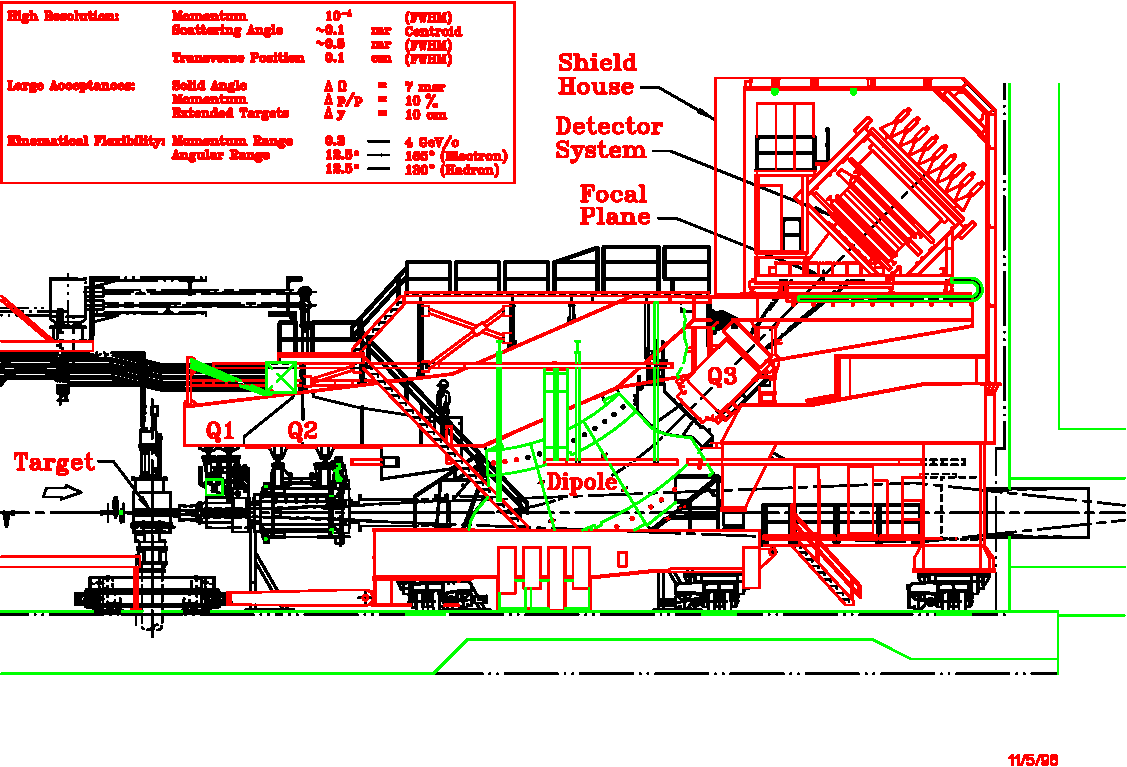
\includegraphics[angle=0,width=0.9\textwidth,clip]{figure0101_r}
\caption[Spectrometers: Elevation View of Hall~A HRS]{A side view of the Hall~A
HRS spectrometer.}  
\label{fig:hrs_ev}
\end{center}
\end{figure}
 
\begin{figure}[tbp]
\begin{center}
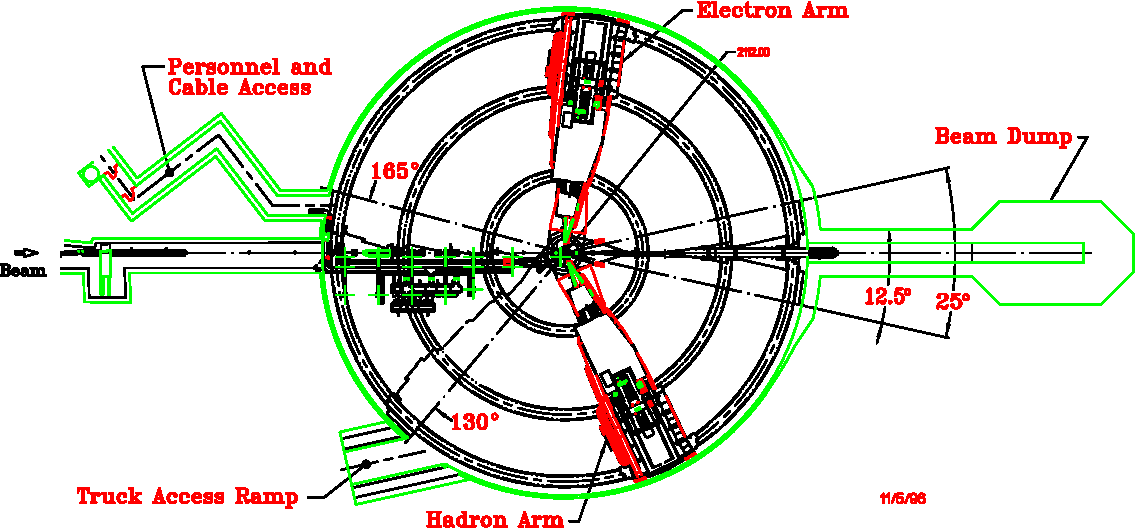
\includegraphics[angle=0,width=0.9\textwidth,clip]{figure0102_r}
\caption[Spectrometers: Plan View of Hall~A]{A bird's eye view of the Hall~A
end-station at TJNAF.}  
\label{fig:hrs_pv}
\end{center}
\end{figure}


A layout of the 4 GeV/c High Resolution Electron Spectrometer is shown 
on Figures~\ref{fig:hrs_pv} and \ref{fig:hrs_ev}.
Its main design characteristics are 
given in the attached table.  The spectrometer has a vertical bending 
plane and 45$^{\circ}$ bending angle.  The QQDQ design includes four 
independent superconducting magnets, three current-dominated 
cos2$\theta $ quadrupoles and one iron-dominated dipole with 
superconducting racetrack coils.  The second and third quadrupoles of 
each spectrometer have sufficiently similar field requirements that they 
are of identical design and construction.  The overall optical length, 
from target to focal plane, is 23.4 m.  Optically, the HRHS 
is essentially identical to HRES. In fact the two spectrometers can be used 
interchangeably to detect either positively or negatively charged particles 
as needed by any particular experiment. They are now commonly refered to 
as ``The Left Arm'' and ``The Right Arms'' rather than ``Hadron'' and ``Electron'' 

The support structure includes all system elements which bear the weight 
of the various spectrometer components and preserve their spatial 
relationship as required for 45$^{\circ}$ vertical bending optics.

The alignment and positioning system includes all the elements which 
measure and adjust the spatial relationship.  The support structure 
consists of the fabricated steel components which support the magnets, 
detector, shield house and associated equipment.  It is composed of the 
box beam, which supports the outer elements in fixed relative position 
atop the dipole; the dipole support bracket, upon which the dipole rests on 
the jacks; the cradle, upon which the dipole rests through the vertical 
positioning system, VPS; and a portion of the shield house load through 
the inboard legs of the gantry; the gantry, which supports the shield 
house and the magnet power supplies; and the bogies, which support the 
cradle-gantry assembly and roll on the floor plates and provide the 
driving power to move the two spectrometer arms.

The detector package (described in detail in Chapter \ref{chap:hrs-det})
is supported on the box beam and is surrounded by 
the shield house.  It must perform two functions, tracking and particle 
identification, PID.  The most important capability of focusing 
spectrometers is measuring precisely the momenta and entrance 
orientations of the tracks.  Momentum resolution of 10$^{-4}$ is 
obtainable, consistent with the resolution of the incident beam.

The actual configuration of the detector package varies from experiment to
experiment. The description given here is only an example of what is possible.
}

\infolevone{
A particle traversing the detector stack 
(Figure~\ref{fig:hrs_electron_det}) encounters two sets of horizontally
mounted, vertical drift wire chambers (x,y) with two planes of 368
wires in each chamber. The track resolution is $\sim$ 100 $\mu$m.  
From the chamber information both 
positions and angles in the dispersive and transverse directions can be 
determined.  The information from these chambers is the principal input 
of the tracking algorithms.

The chambers are followed by a scintillator hodoscope plane designated S1. 
This plastic scintillator array provides the timing reference for 
the drift chambers, and is also used in trigger formation and in combination 
with a second hodoscope pair it can provide time of flight particle 
identification.  These scintillators can also be used to perform crude 
tracking.

The next element encountered by a particle is a gas threshold \Cherenkov{} 
detector.  This is used for particle identification.  This gas threshold \Cherenkov{} detector can be swapped 
against an Aerogel detector, with a similar function.

The second hodoscope plane, S2, is located directly behind the 
gas \Cherenkov{}.  Its function is essentially the same as that of S1.  
In the hadron spectrometer an option exists to have this hodoscope 
pair be preceded by a third chamber, to improve tracking.
 Each of the two spectrometers 
have gas and Aerogel \Cherenkov{} detectors which can be used
 when they are in electron detection mode.

The final elements in the detector stack on HRSE are 
the pre-shower and the total-absorber lead glass shower 
calorimeter.  This is used for energy determination and PID.

\begin{figure}[tbp]
\begin{center}
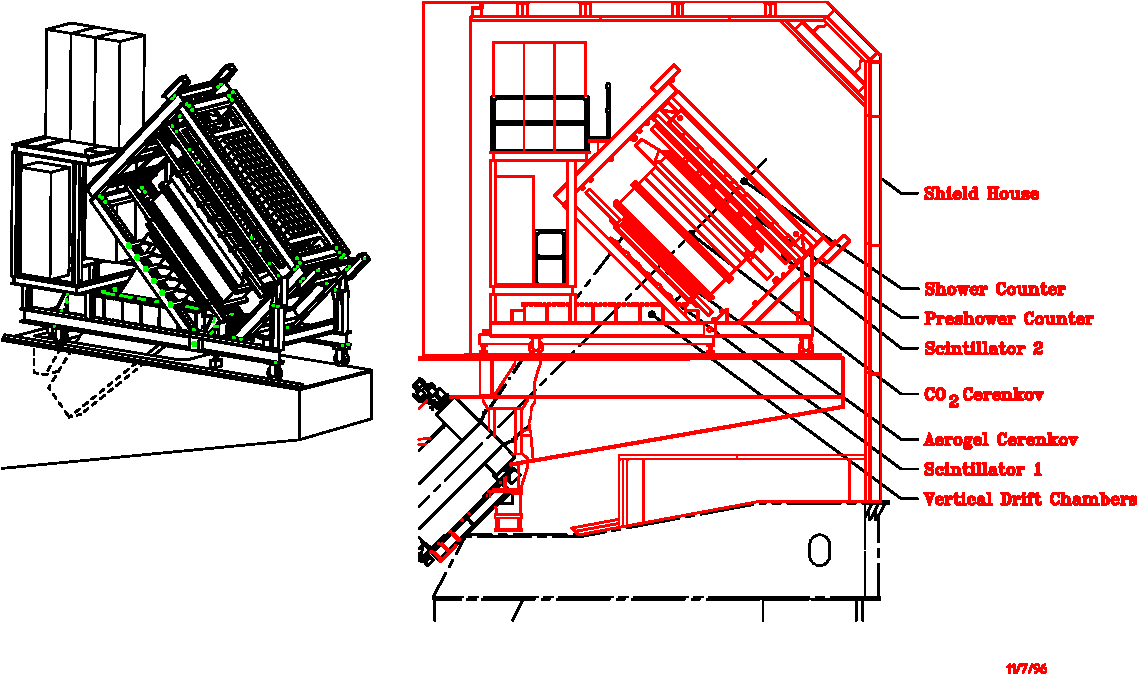
\includegraphics[angle=0,width=\textwidth,clip]{figure0103_r}
{\linespread{1.}
\caption[Spectrometers: Electron Arm Detectors]{The electron spectrometer detector stack.}
\label{fig:hrs_electron_det}}
\end{center}
\end{figure}

\begin{figure}[tbp]
\begin{center}
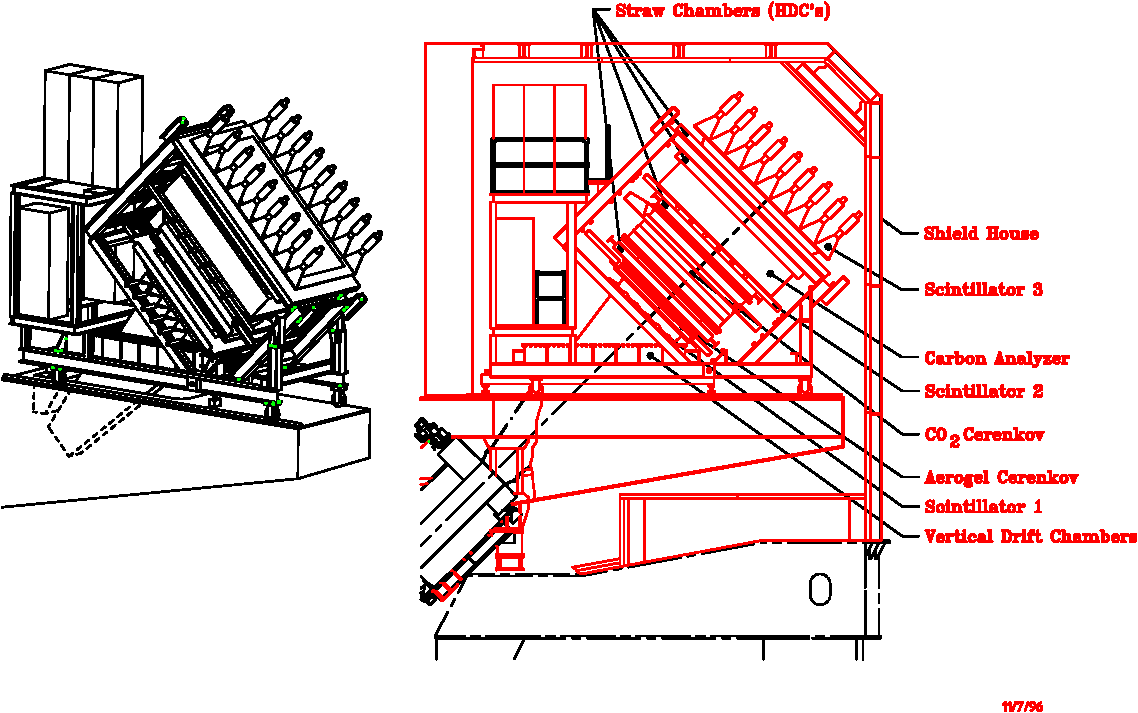
\includegraphics[angle=0,width=\textwidth,clip]{figure0104_r}
{\linespread{1.}
\caption[Spectrometers: Hadron Arm Detectors]{The hadron spectrometer detector stack.}
\label{fig:hrs_hadron_det}}
\end{center}
\end{figure}


The hadron detector is shown schematically in 
Figure~\ref{fig:hrs_hadron_det}.  It consists 
of two sets of (x,y) vertical drift wire chambers identical to those of the 
electron arm.  The remaining part of the detection system is used to 
define the level 1 trigger, as well as for particle identification and 
timing.  It consists of two minimally segmented planes of 
scintillation counters equipped with photomultipliers at both ends, and 
it includes \Cherenkov{} counters (gas CO$_2$ and Aerogel).

In addition, a proton polarimeter is installed in the back of the 
detector package to measure the polarization of the proton using a 
segmented carbon analyzer up to 60 cm in thickness to allow measurements 
over a wide range of proton energies.  A pair of front and a pair of 
rear straw tube wire chambers determine the incident and 
scattered angles, respectively.  The 
polarimeter detectors are dimensioned to accept a 20$^{\circ}$ cone of 
scattered protons.

Several support systems are necessary in addition to the basic 
components mentioned above.  They include gas supply systems for the 
wire chambers, high voltage supplies, readout electronics, a second 
level trigger, software for data analysis and testing, and a remotely 
controllable mechanical system.

For each spectrometer, all detectors are mounted on a 
single rigid support frame along with their associated electronics.  The trigger electronics are located on the support frame, next to the detectors.

To reduce the resolution degrading effects of multiple scattering, the 
entire interior of the spectrometer from the collimator box to the detector hut 
is a vacuum vessel.  The ends of this evacuated volume are capped by 
relatively thin vacuum windows.
}

\begin{safetyen}{0}{0}
\section{High Resolution Spectrometers}
\label{sec:hrs-safety}
\end{safetyen}

The principle concern with the spectrometers is that they are large, 
and have associated vacuum, hydraulic, cryogenic and magnet systems all of 
which can be potentially dangerous.

The bogies which move the massive 1200 ton spectrometers must be 
carefully operated.  Inspection of the floor and wheels to ensure there is no 
debris which the wheels could ride over is mandatory.  Similarly 
personnel need to be aware that the spectrometers are moving so that no one 
inadvertently gets trapped.

The vacuum systems associated with the spectrometers are essentially 
pressure vessels (see Chapter \ref{chap:vacuum} for more details).
Care should be exercised so as not to puncture the 
windows.

The magnets themselves are installed inside cryostats.  These vessels 
are exposed to high pressures and are therefore equipped with safety 
relief valves and burst discs.

The hydraulic system originally intended to operate the vertical positioning system (VPS) 
and the horizontal positioning system (HPS) has effectively been dismantled, after problems were encountered during the initial attempted operation of the system.

The cryogenic system operates at elevated pressure at 4K.  One must 
guard against cold burns and take the normal precautions with pressure 
vessels when operating this system.  Only authorized personnel are permitted to install 
and take out U tubes.

The magnets have a great deal of stored energy as they are large 
inductors. Always make sure people are clear of them and that
the dump resistor is attached to the magnet.

There are several major safety concerns with regards to the detectors, 
namely 1) flammable gas located in the VDC, 2) ODH hazard due to 
CO$_2$ in the \Cherenkov{} counter, 3) high voltage due to the photo 
multipliers on the various detectors and 4) a thin vacuum window 
separating the detector array from the vacuum system in the 
spectrometers.

\infolevltone{
\begin{safetyen}{5}{10}
For more information consult the full OSP manual~\cite{HallAosp}.
\end{safetyen}
} %infolev

\begin{safetyen}{10}{15}
\subsection{Authorized Personnel}
\end{safetyen}

In the event that problems arise during 
operation of the magnets, qualified personnel should be notified
(see Table \ref{tab:hrs:personnel}).  
This includes any prolonged or serious problem with the source of magnet 
cryogens (the ESR).  On weekends and after hours there will be a 
designated individual on call for magnet services.  Any member of the 
Hall A technical staff is qualified to deal with unusual magnet 
situations but in the event of serious problems the technician on
call should be contacted.

\begin{namestab}{tab:hrs:personnel}{HRS: authorized personnel}{%
      HRS: authorized personnel. ''W.B'' stands for the white board 
      in the counting house.}
   \TechonCall{\em Contact}
   \EdFolts{}
   \JackSegal{}
   \HeidiFansler{}
   \JessieButler{}
   \AndrewLumanog{}
   \JasonGlorioso{}
   \MahlonLong{}
\end{namestab}

\infolevone{
\section{The Magnets of HRS}

Each HRS is composed of three superconducting quadrupole magnets, Q1, Q2, 
and Q3, and one superconducting dipole magnet.  The large quadrupoles were 
manufactured for JLab by SIEMENS, the small quadrupole by SACLAY, while 
the dipole was built for JLab by WANG NMR.  The quadrupole magnets are 
referred to as Q1, Q2, and Q3, where a particle first traverses Q1, then 
Q2 and the dipole magnet and finally traverses Q3.

The magnet system is followed by a large steel and concrete detector 
hut, in which all detector elements reside.  Most of the 
detector elements have been built by universities involved in the Hall A 
physics program.

The HRS magnet system is the cornerstone of the Hall A activities.  
Many of the experiments approved in Hall A center on physics at high 
resolution and other short-range phenomena, and rely on a spectrometer 
able to momentum analyze charged particles up to very high momenta.  The 
design value for the maximum momentum accessible to the HRS magnet 
system is 4 GeV/c.
}

\subsection{Magnets and Power Supplies}

\infolevone{
The HRS magnet's are all superconducting and hence their coils must be 
maintained at cryogenic temperatures during operations.  The LHe 
required by the magnets is supplied by the End Station Refrigerator, ESR.

All the HRS magnets cryogenic services are supplied through the overhead 
cryogenic lines.  The distribution network begins at the distribution 
box over the pivot.  This box is connected to the rest of the network 
via the flexible transfer lines over the pivot.  The network is adjacent 
to the upstairs catwalk of the HRS.

Cryogenic information about each magnet is available on the control 
screens in the counting house, one for each magnet.  Normally during run 
periods the control screens are sent upstairs to the Hall A counting 
house and information on all the HRS magnets is available on the HRS 
control screen located in the center of the main console.  The control 
of all magnets is described in a following Section.

The power supplies for the magnets are located on the gantry balcony 
adjacent to the magnets.  The supplies are all cooled with low conductivity water (LCW).
}

\begin{safetyen}{10}{15}

Under no 
circumstances should any panel of any magnet power supply be opened by someone 
other than authorized personnel.  There are also 
signs posted listing the dangers of high magnetic fields.
\end{safetyen}

\infolevone{
A control interface for the power supplies is available through the 
HRS control screen in the Hall A counting house.
}

\infolevone{
\subsection{Quadrupole Magnets}

The quadrupoles provide some of the 
focusing properties of the spectrometer and to a large extent 
its acceptance.  Operating limits imposed on the 
quads are as follows: 1850A for Q2 and Q3 and 3250A 
for Q1.

All three quadrupoles for the HRS spectrometer are warm iron 
superconducting magnets.  The soft iron around the superconducting coil 
enhances the field at the coil center and reduces stray fields.  The 
basic parameters for the first quadrupole, Q1, are an effective length of about 
0.9 $m$, useful aperture of 0.3 $m$ and a field gradient of 9.5 
T/m.  To achieve the lowest possible angle setting of the HRS 
spectrometer (with respect to the beam line) the incident electron beam passes through
a notch in the outer yoke of Q1 when the spectrometer is at
its smallest angle of 12.5$^\circ$ . The 
other two quadrupoles, Q2 and Q3, are essentially identical with an 
effective (magnetic) length of about 1.8 meter, a useful aperture of 
0.6 $m$ and a field gradient of 3.5 T/m.
}

\infolevthree{
The maximum operating currents (assuming a 4 GeV/c momentum particle) 
for the quadrupoles are about 3000 A, 1700 A, and 1600 A, for Q1, Q2, and 
Q3, respectively.  This will render pole field values 
of 1.2, 1.0, and 1.0 T, respectively.  The energy stored in the 
quadrupole fields is sufficient to cause an unrecoverable quench if all 
the energy stored is dumped into the magnets.  Therefore a quench 
protection circuit is incorporated.  However, a quench can only happen 
if the cryomagnets have a helium level below the coil 60\% during operation.

The operating current to the Q1 quadrupole coils is provided by Danfysik 
System 8000 power supplies, which can operate up to 3500 A current and 5 
V.  The power supplies will be cooled with a combined maximum 
water flow of 45 liters per minute.

In addition to the main quadrupole windings, all quadrupoles have 
multipole windings.  To further optimize focusing properties of the HRS 
magnet system, it was intended to operate including some of these multipole 
trim coils in order to reduce higher order aberrations.
The operating current for these multipole corrections would be 
small, only (the multipole corrections are typically less than 2\% of 
the main quadrupole field), of order 50 A. Since the sextupoles were inadvertently 
installed rotated 90 $^\circ$ from their correct
orientation, these trim coils are now considered useless 
and there are at present no plans to use them.

\subsection{Cryogenic Procedures}

The cryogenics control is handled by the JLab Cryogenics Group.  The cryo control coordinator 
can be reached at the CHL (x7405) or by calling the MCC.

\subsection{First Time Startup Check List.}  

See attached check lists for all quadrupole and dipole magnets
 (Tables~\ref{tab:dip_check}, \ref{tab:q1_check}, and \ref{tab:q23_check}).
} %infolev

\infolevone{
\subsection{Dipole Magnet}

The dipole, by virtue of its field index, provides both
dispersion and focusing.  The present operations envelope 
states that the supply for the left HRS dipole may not be
operated at a current above 1800 A (4.4 GeV/c). The supply for the right HRS
dipole may not be operated above 1200 A (3.2 GeV/c), due to complications
caused by an internal short. 

The dipole for the HRS spectrometer is a superconducting, cryostable 
magnet.  Its basic parameters are an effective length of about 6.6 $m$, a 
bend radius of 8.4 $m$, and a gap width of 25 $cm$.  It is configured to 
achieve a 45 degree bending angle for 4 GeV/c momentum particles at a 
central field excitation of 1.6 T.  For the HRS dipole to reach 1.6 T 
an operating current of about 1500 A is required.
} %infolev

\infolevthree{
The dipole has been designed to achieve cryostability up to a field of 2 
T, and this property has been extensively tested up to a field of 1.6 T. 
 The cryostable coils are equipped with an energy removal circuit to 
cover the possibility of an unrecoverable quench.  However, this can 
only happen if the helium level drops below the coil during operation.  
The current to the coils will be provided by a Dynapower Corporation power 
supply, which can operate up to 2000 A and 10 V.  This 
power supply is located on the gantry beside the dipole, and will be 
cooled with a maximum water flow of 35 liters per minute.
The total water flow needed to cool the 4 power 
supplies for the HRS magnet system (dipole and quadrupoles) amounts to 
80 liters per minute, with a supply pressure of cooling water for Hall A 
of 100 psi.
} %infolev

\infolevtwo{
\section{Operation of the HRS Magnets}

\subsection{Introduction}

This is an abbreviated operating manual for 
the HRS superconducting magnets specifically designed for Hall A 
experimenters.  It provides instructions for setting currents, invoking 
NMR field regulation and general system monitoring.  Curious readers are 
directed to the references for more in-depth operating instructions and 
other technical manuals. Copies of the following supporting
documents are available in the Hall A Control Room and through the Hall A webpage
(see Table~\ref{tab:hrs-mag-manuals}).

\begin{table}[htp]
\begin{center}
\begin{tabular}{|l|l|}
\hline
References & \\
\hline 
WANG NMR Dipole & User Manual \\
Dynapower & Instruction Manual \\
Appendix & NMR Tesla meter \\
Appendix & NMR Field Regulation \\
Siemens/Fug & Q2/Q3 Magnet Instrumentation and Power Supplies \\
Saclay/Danfysik & Q1 Power Supply Manual \\
TOSP & HRS Dipole \\
TOSP & HRS Quadrupole Q1 \\
TOSP & HRS Quadrupole Q2, Q3 \\
HRS & SC Dipole Magnet Safety Review Vol. 2 \\
HRS & SC Quad Safety Review Vol. 1 \\ \hline
\end{tabular}
\end{center}
\caption[HRS Magnets: extra manuals]{HRS Magnets: extra manuals available in 
     Hall A Control Room.}
\label{tab:hrs-mag-manuals}
\end{table}

\subsection{Simple HRS Setting (Autopilot Mode)}
\label{sec:hrs-mag-set} 

 The magnets are controlled remotely using EPICS~\cite{EPICSwww} and
 EDM~\cite{EDMwww} GUI, provided that everything is working and power 
 supplies are turned on and ready to go.
 The appropriate interface runs
 on the computer \mycomp{hacsbc2} (see Section \ref{sec:contr-ha-menu}).
 On the ``Hall A General Tools'' control screen, in the upper left, there is 
 a rectangular box for each spectrometer (see Figure~\ref{fig:hrs_mag_cntrl}). 
\begin{figure}
\begin{center}
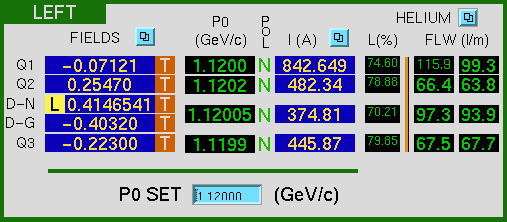
\includegraphics[angle=0,width=0.8\textwidth]{medm_halla_tools_1_cut1}
{\linespread{1.}
\caption[HRS: Magnets control]{A part of ``Hall A General Tools'' screen, 
        used for HRS (left) magnets control.}
\label{fig:hrs_mag_cntrl}}
\end{center}
\end{figure}

This box displays a brief summary of the status of the spectrometer
magnets and their cryogenic systems. The blue fields (with white
numbers) give readbacks of the magnetic fields and currents in each
magnet. The black fields also give readbacks, however in this case if
the text appears green those parameters are OK while if they are red
then that parameter is out of tolerance and may indicate a fault
condition. For example if the helium level goes below a certain point
the magnet will be automatically turned off.  In some cases it may be
desirable to monitor certain critical quantities on a strip chart
(e.g. magnet settings). A strip chart tool is available for this
purpose from the bottom of the ''EOS Menu'' button in the ''MyMenu'' window.

{\bf To set the spectrometers} for a given value of central momentum
(P0) type the desired P0 value into the light blue P0 SET box and hit
return. The magnets will be automatically 
set to the correct
values. All green numbers in the P0 column indicates that the desired
field or current settings have been reached. 

{\bf Caution:} Regarding the
dipoles, in general it's a bad idea to assume that at the first
instant that the P0 display turns green that the desired field has
been reached and you can start taking data. Stable field is in general
not achieved for from 15 to 30 minutes after reaching the nominal
desired field. This settling time depends on the magnet (the right dipole is
slower than the left dipole) and the magnitude of the field change (small
changes settle faster than big changes). Experimenters are advised to
observe both the field reading and current reading on the magnet in
question and verify that things are stable to their satisfaction
before proceeding.
 
\subsection{Powering Up Dipole Magnets:}

Use these instructions to recover from loss of a magnet due to a fault
(e.g. He level or lead flow fault). The order of actions matters. \\
(Contact Tech-On-Call if anything behaves funny or things don't
respond as expected. Sometimes after a trip an access to the Hall is
required to reset things).

\begin{list}{\arabic{enumi}.~}{\usecounter{enumi}\setlength{\itemsep}{-0.15cm}}
   \item Wait for Iout=0 (you can't and don't want to do anything while the magnet is in emergency fast dump mode.)
   \item While waiting, make a log entry re the fault. Give details such as time, coincident activities, and nature of the fault.
   \item Make sure the fault is cleared. (e.g. He level and flow rates returned to normal values and stable)
   \item In the HRS Right (Left) Dipole Systems' control panel:
   \begin{list}{}{\setlength{\itemsep}{-0.15cm}}
      \item[(a)] Press RESET (verify that all faults are cleared in the middle column)
      \item[(b)] Press ON (Display will indicate Power Supply ON and Magnet ENGAGED)
   \end{list}
\end{list}


Power supply and magnet are ready to go. From here you can return 
to "Autopilot Mode" (see Section \ref{sec:hrs-mag-set}).

\subsection{Starting Q1 Power Supply:}

 Do this when a fault causes the power supply to shut off.
 Wait for fault to clear (watch He levels). 
\begin{list}{\arabic{enumi}.~}{\usecounter{enumi}\setlength{\itemsep}{-0.15cm}}
   \item Push POWER OFF/RESET (check all faults cleared)
   \item Select desired polarity
   \item Push POWER ON
   \item Type in Setpoint (Amps) (light blue field) or re-enter P0 in Autopilot Mode.
\end{list}

\subsection{Starting Q2/3 Power Supply:}

 Do this when a fault causes the power supply to shut off.
 Wait for cause of fault to clear (watch He levels). 
 \begin{list}{\arabic{enumi}.~}{\usecounter{enumi}\setlength{\itemsep}{-0.15cm}}
   \item Push RESET 
   \item Select desired polarity
   \item Push ON
   \item Type in Current Set (light blue field) or re-enter P0 in Autopilot Mode.
\end{list}

} %infolev

\subsection{Rotation}
%
% Thanks to John LeRose for Rotation text. 07NOV2013
%
Moving an HRS
Since each HRS weighs in excess of 1,000 tons it is very important that all safety
precautions are carefully adhered to. The good news is they move very slowly (a few degrees/min
maximum), BUT 1,000 tons moving even very slowly is hard to stop. 

Hazards include:
\begin{itemize}
\item{Knocking items over.}
\item{The wheels crushing things (including fingers and toes) on the floor in the path of the 
spectrometer}
\item{Damaging the beamline or other equipment on the floor if one goes to too small 
or too large an angle, or if it just gets pushed around inadvertantly.}
\item{Tearing out of cables etc. physically attached to the superstructure}
\end{itemize}

Hazard mitigations:
\begin{itemize}
\item{Guards on either side of the wheels prevent items from getting under them.}
\item{Large pins in the floor to stop the spectrometer rotated beyond the needed angular range.}
\item{Blinking lights on the spectrometers indicating they are in motion or that motion
is possible (controls engaged etc.)}
\item{During a running experiment the run coordinator and work coordinator should know in advance 
of any moves.  Moves at any other time must be cleared with the Hall work coordinator 
before implementation.}
\item{Careful inspection of the intended path to make sure it is clear. This is part of
the pre-run checklist performed by the technical staff prior to closing the Hall and
a remote camera allows shift worker to inspect the area.}
%
%\item{Any motion that takes a spectrometer inside 14 degrees or outside x degrees
%(x being specified in the pre-run checklist and noted on the whiteboard during a run) 
%must be supervised by a trained Hall A technician.}
\end{itemize}

\infolevone{
Remote Procedure for a shift worker:
\begin{itemize}
\item{Make sure the move is part of the approved runplan (if in doubt, check with the 
run coordinator).}
\item{Check that the pre-run checklist has been completed and note and comply with any 
possible limitations to spectrometer motion (if there is a conflict inform the Run
Coordinator and do not initiate any move until the conflict is cleared).}
\item{Visually inspect the Hall using the closed circuit TV cameras to verify that there
are no obstructions.}
\item{If people are in the Hall wait until they leave (during a Controlled Access MCC keeps
track of people in the Hall). (Maybe we could soften this to "Inform EVERYONE in the Hall of
the move".)}
\item{Activate the spectrometer motion controls (see the Wiki and below) and 
move to the desired angle.}
\item{Deactivate the controls (brakes on, power off, etc.)}
\item{Update the spectrometer position information on the Hall A Controls screen}
\item{Make a halog entry indicating you've moved the spectrometer including from what angle 
to what new angle.}
\end{itemize}

Procedure for a non-run associated move in the Hall:
\begin{itemize}
\item{Inform the work coordinator of the planned move}
\item{Perform a careful visual inspection to verify that the path is clear}
\item{Check to make sure there are no temporary connections to the spectrometer (wires etc.)
that could be damaged during the move.}
\item{Inform everyone in the Hall of the move and check with them re 3.}
\item{Activate the spectrometer motion controls (see the Wiki and below) verify 
that the warning lights are on and move to the desired angle.}
\item{Deactivate the controls (brakes on, power off, etc.).}
\end{itemize}

The full proceedure for moving the spectrometer follows and can also be found on the Hall A wiki.

On hacsbc2, click the red "tool box" icon on the linux taskbar, as above. Choose 
bogies\_SetSpec so that you can determine the angle and vernier setting for the spectrometer.
Enter the spectrometer (L or R), and the angle, and you will get two options for the floor 
mark and the vernier. Generally choose the vernier closer to zero. Center the cameras on the 
desire vernier using the Move+/Move- buttons on the Hall A General Tools screen. The TV monitors 
for these cameras are on the middle shelf, in rack CH01A05.

Choose bogies\_Left (or bogies\_Right) in the tool box to bring up the bogies control screen. 
Click PSM enable and wait a few seconds for PSM OK to read YES. 
Click DM enable and wait a few seconds for DM OK to read YES.
Make sure the velocity is set to 0 and the direction is CW or CCW as desired. Click on Brake Release 
and wait for Brakes OK to read YES.

Click on ClampRelease, set the velocity to 700. Once you see the spectrometer start to move in the 
floor angle camera - you cannot see the spectrometer move in the Hall overview camera, as it only 
moves a few degrees per minute at maximum speed. For the left arm, to move to a larger angle, the 
direction should be CCW, while for the right arm CW moves the spectrometer to larger angle. The 
direction of the spectrometer is reversed by using a negative rpm. Watch the spectrometer motion 
on the cameras. When you are getting close to the desired angle, slow down to about 300 rpm. 
To stop, click on the Clamp Release button and the Brake button. Disable DM and PSM, and disconnect 
to close the GUI. Read off the floor angle mark and vernier, and input the values into the appropriate 
fields in the Alignment section of the Hall A General Tools GUI. 
}









\newpage
\section[Field Monitoring]{Field Monitoring
\footnote{
  $CVS~revision~ $Id: nmr-1999.tex,v 1.4 2003/12/17 03:59:48 gen Exp $ $ 
}
\footnote{Authors: J.LeRose \email{lerose@jlab.org}}
}

The field-monitoring controls are available using the main 
HRS screen%
\infolevtwo{ (see Figure~\ref{fig:hrs_mag_cntrl})%
}. % infolev
The dipoles' field is measured using NMR Teslameters and
field probes.

\infolevone{ 
 
\subsection{ Dipole Field Monitoring Electron Arm}

\noindent {\bf Basic Setup}

Each spectrometer dipole magnet is equipped with a Metrolab PT 4025 
NMR Teslameter, several field probes, and multiplexers (to allow switching 
between the probes).  Details of the operation and theory of operation 
for the Teslameter can be found in its user manual, 
a copy of which is available in the the counting house.
The basic layout is shown in Figure~\ref{fig:nmrbasic}


\begin{figure}
\begin{center}
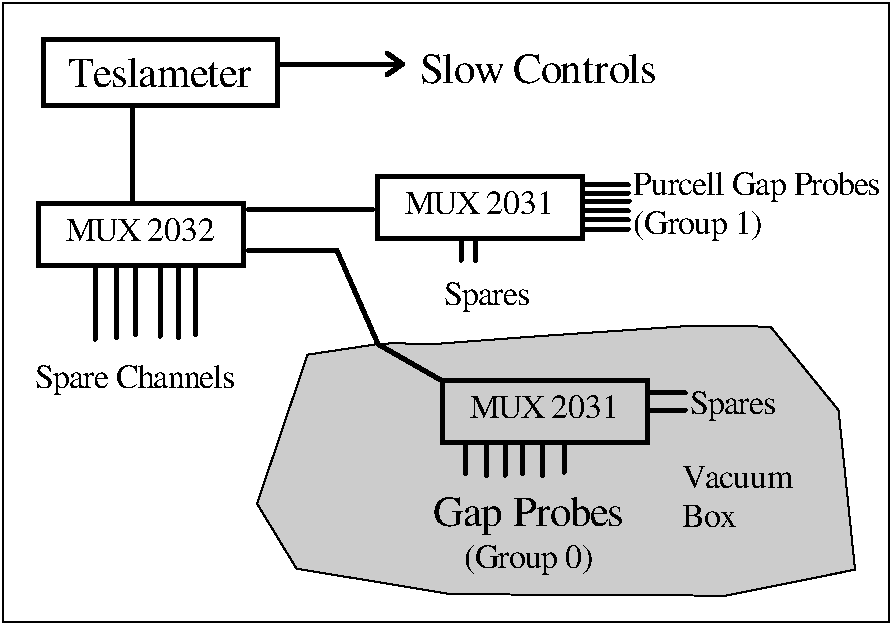
\includegraphics[angle=0,width=15cm,clip]{lerose_fig1}
{\linespread{1.}
\caption[Spectrometers: NMR System Layout]{Basic layout of NMR system}
\label{fig:nmrbasic}}
\end{center}
\end{figure}


 The "Gap Probes" (Group 0 in the controls) are located in two groups 
of three; one group on the low field side of the gap and the other on the high 
field side of the gap.  The groups of three are made up of one each of 
the manufacturer's type 3, 4 \& 5 probes, designed to cover different 
field ranges (see Table \ref{nmr_range}).  The six ``Purcell Gap Probes'' (Group 1 in 
the controls) are located in the Purcell gap of the magnet 
and consists of two each of the above types. {\em Note: Since
the fall of 1998 the multiplexer-multiplexer in both arms,
MUX 2032, has been removed and hence the ``Purcell Gap Probes'' are currently
unavailable. There are no plans to re-install this multiplexer.}

 The "Gap Probes" are equipped with coils which provide a field 
gradient that cancels out the field gradient of the magnet in the vicinity of 
the probe.  These gradient compensating coils are part of a simple circuit 
that is completely independent of the Teslameter.  The basic circuit for 
the compensating coils is shown in Figure~\ref{fig:nmrcir}


\begin{figure}
\begin{center}
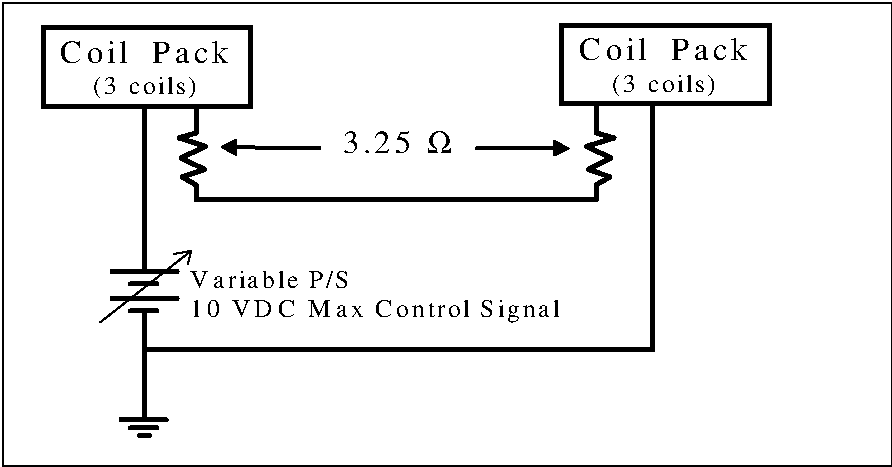
\includegraphics[angle=0,width=10cm,clip]{lerose_fig2}
{\linespread{1.}
\caption[Spectrometers: NMR Gradient Compensation]{Gradient Compensating Circuit.}
\label{fig:nmrcir}}
\end{center}
\end{figure}


%\snfig{figs/lerose_figcce.eps}{Control Voltage calibration for
%Electron Dipole }{nmrcomp4}{5in}

\begin{figure}
\begin{center}
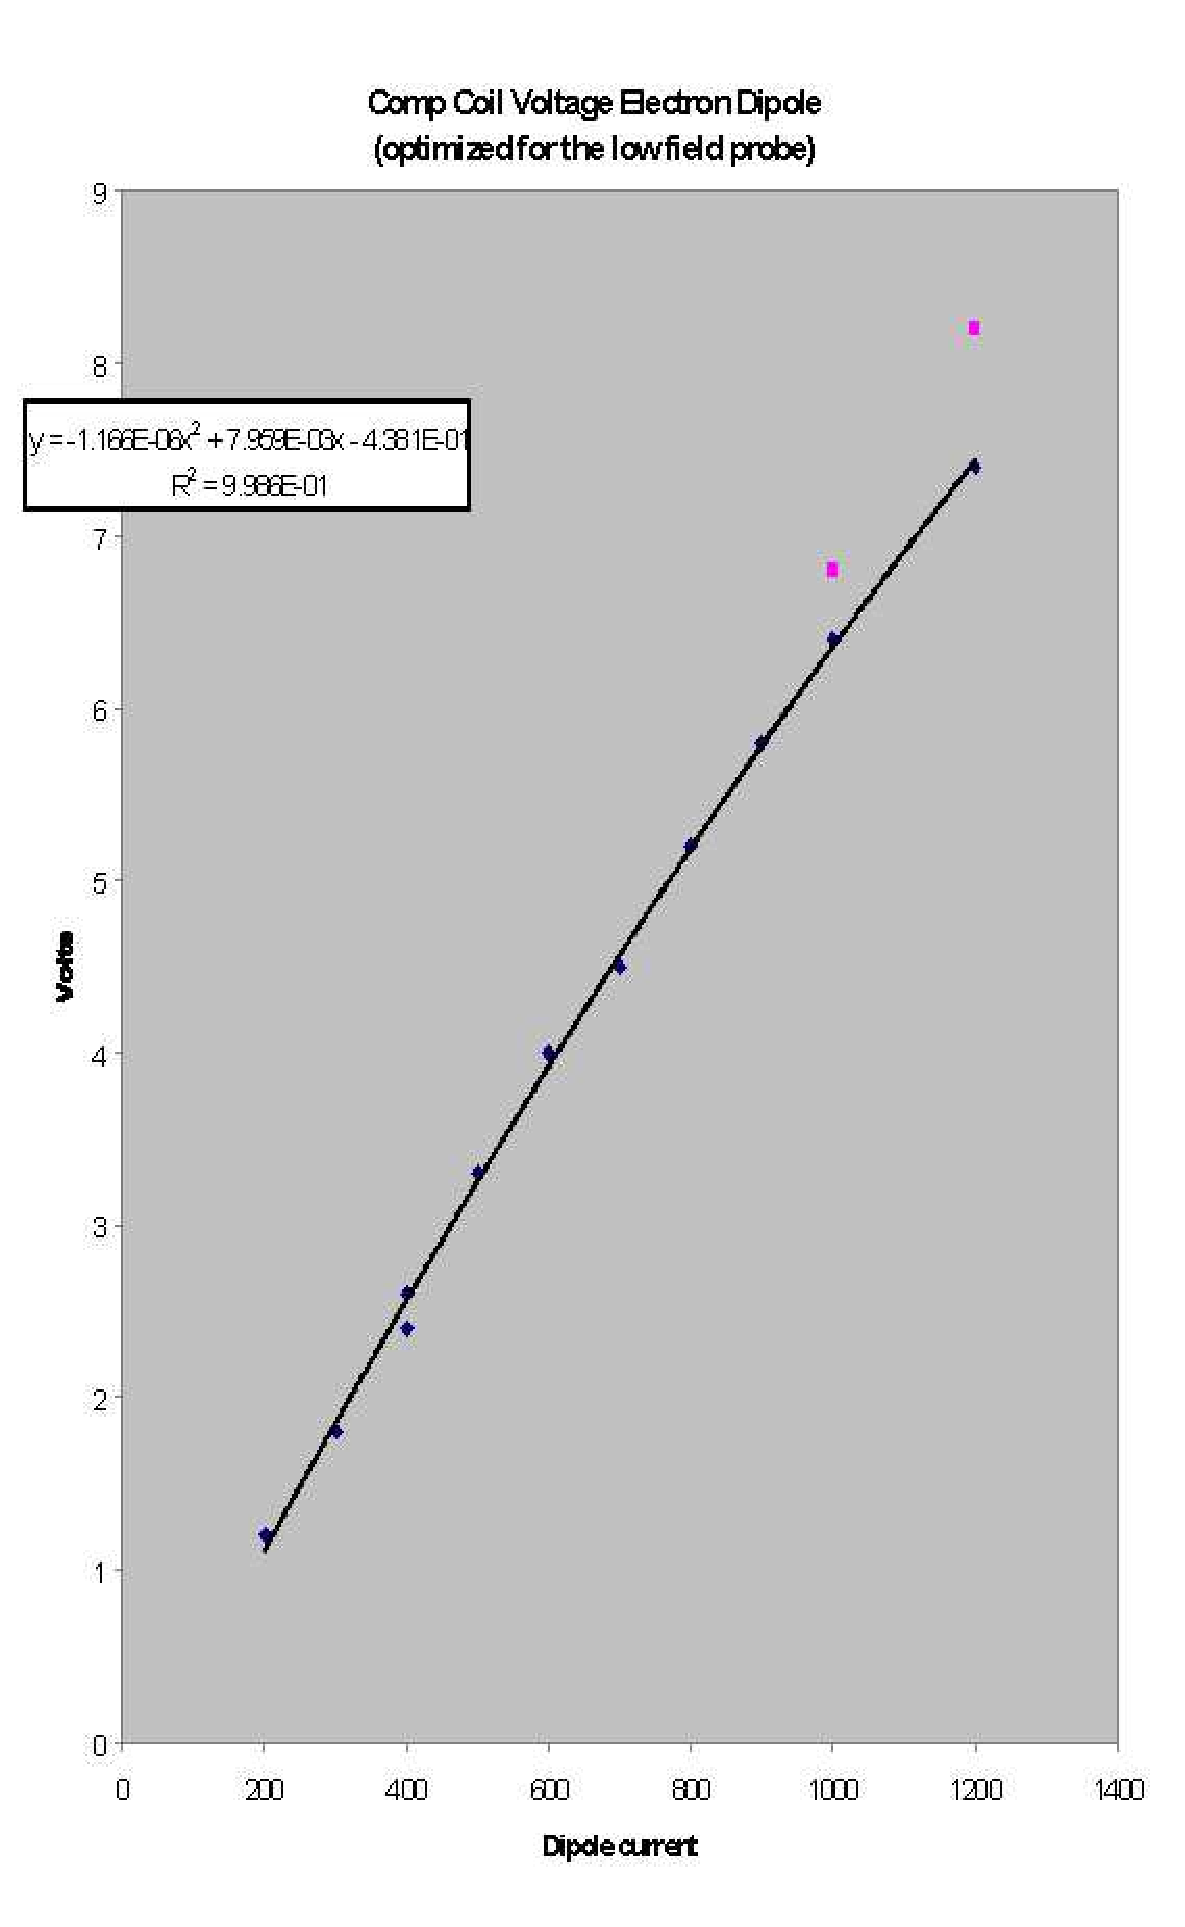
\includegraphics[angle=0,height=20cm,clip]{lerose_figcce}
{\linespread{1.}
\caption[Spectrometers: Control Voltage Calibration for Left Dipole]{Control Voltage calibration for the Left Dipole.}
\label{fig:nmrcomp4}}
\end{center}
\end{figure}

%\snfig{figs/lerose_figcch.eps}{Control Voltage calibration for
%Hadron Dipole }{nmrcomp5}{5in}
\begin{figure}
\begin{center}
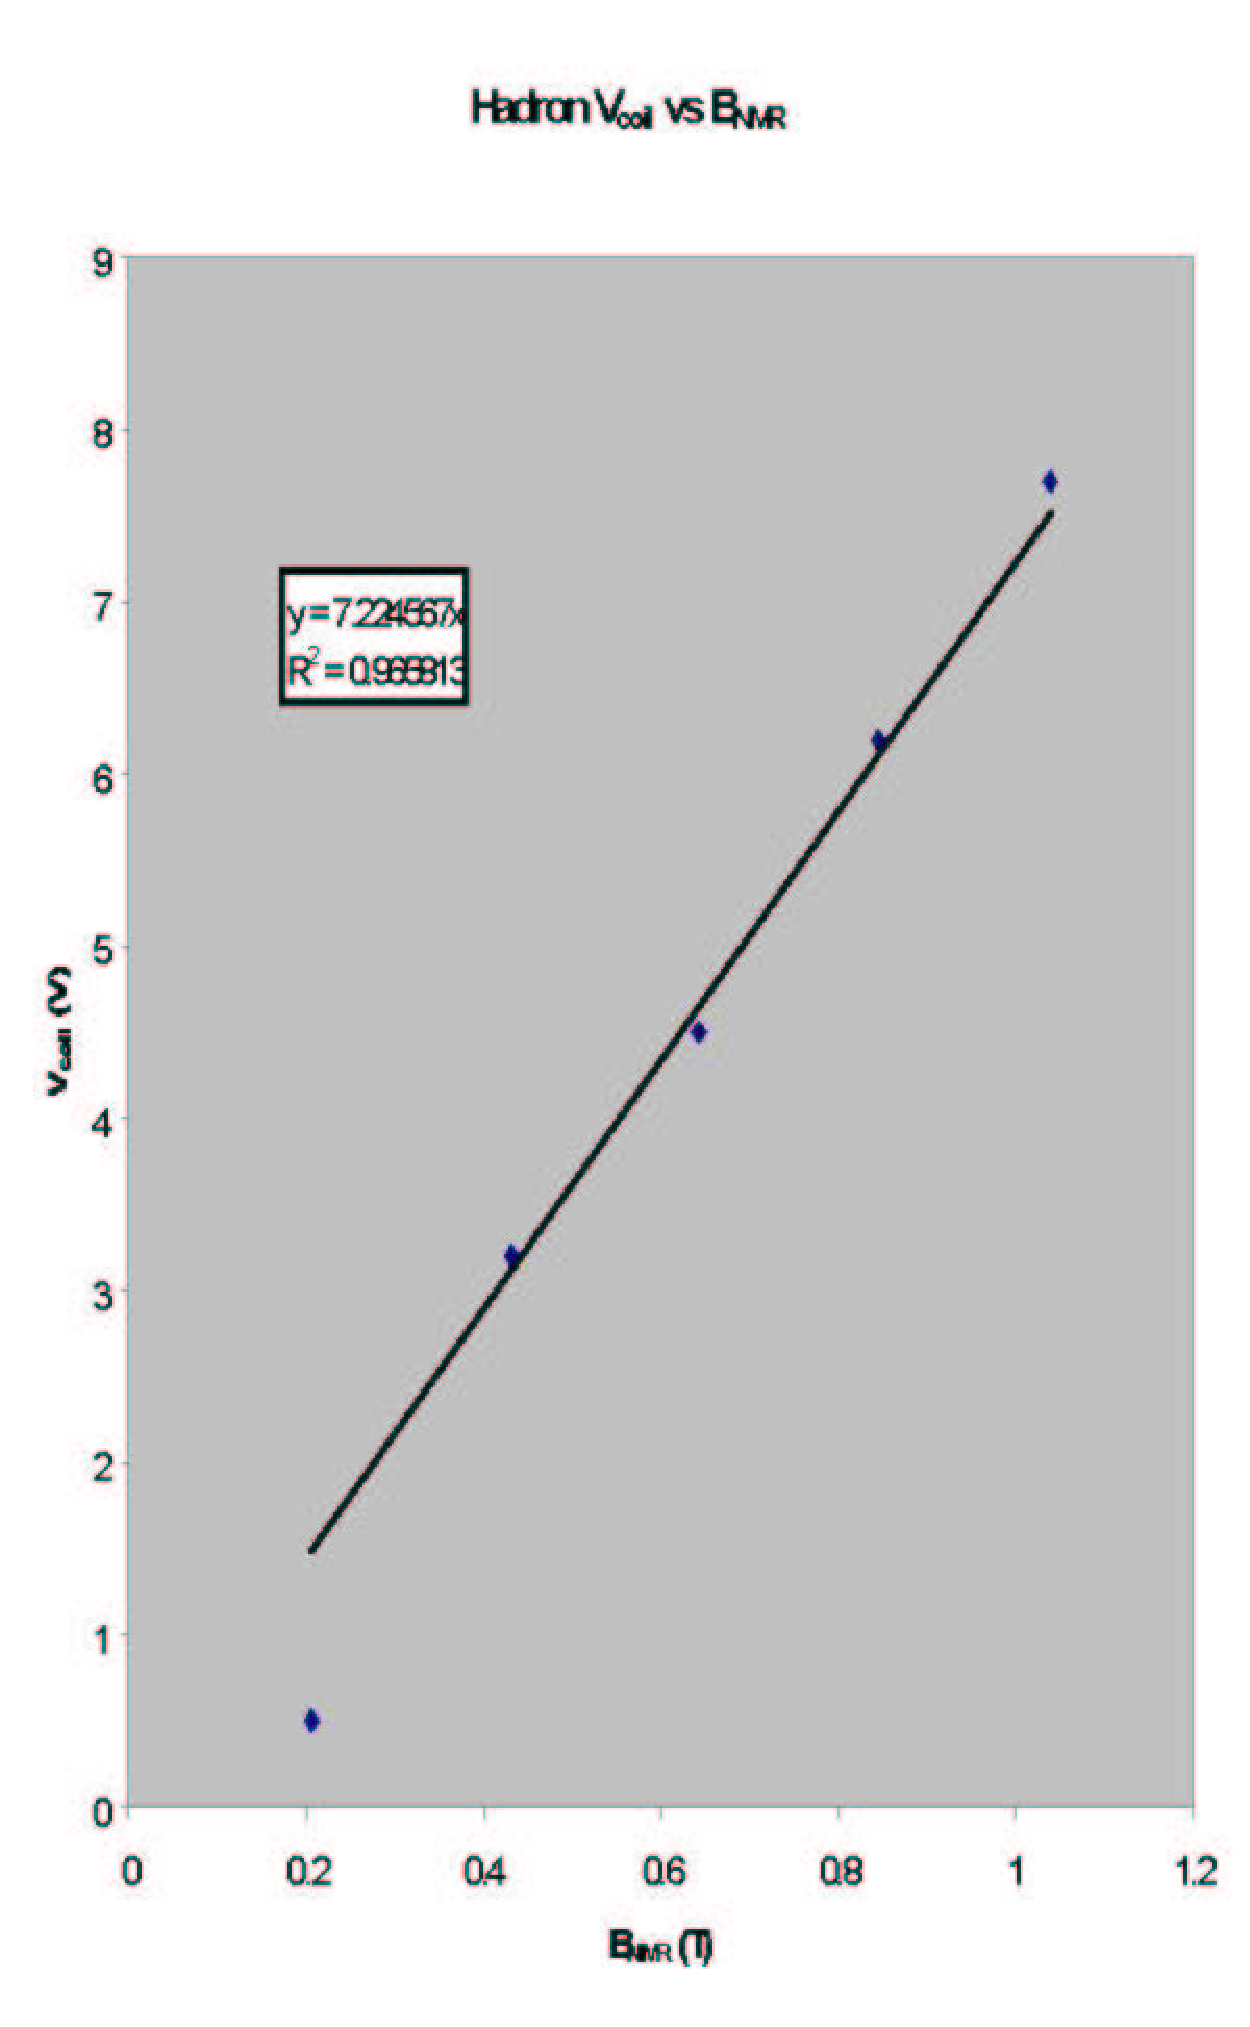
\includegraphics[angle=0,height=20cm,clip]{lerose_figcch}
{\linespread{1.}
\caption[Spectrometers: Control Voltage Calibration for Right Dipole] {Control Voltage calibration for the Right Dipole.}
\label{fig:nmrcomp5}}
\end{center}
\end{figure}

%\snfig{./figs/lerose_fig7.eps}{DAC Calibration for manual operation of NMR probes}{nmr_dac}{9in}
\begin{figure}
\begin{center}
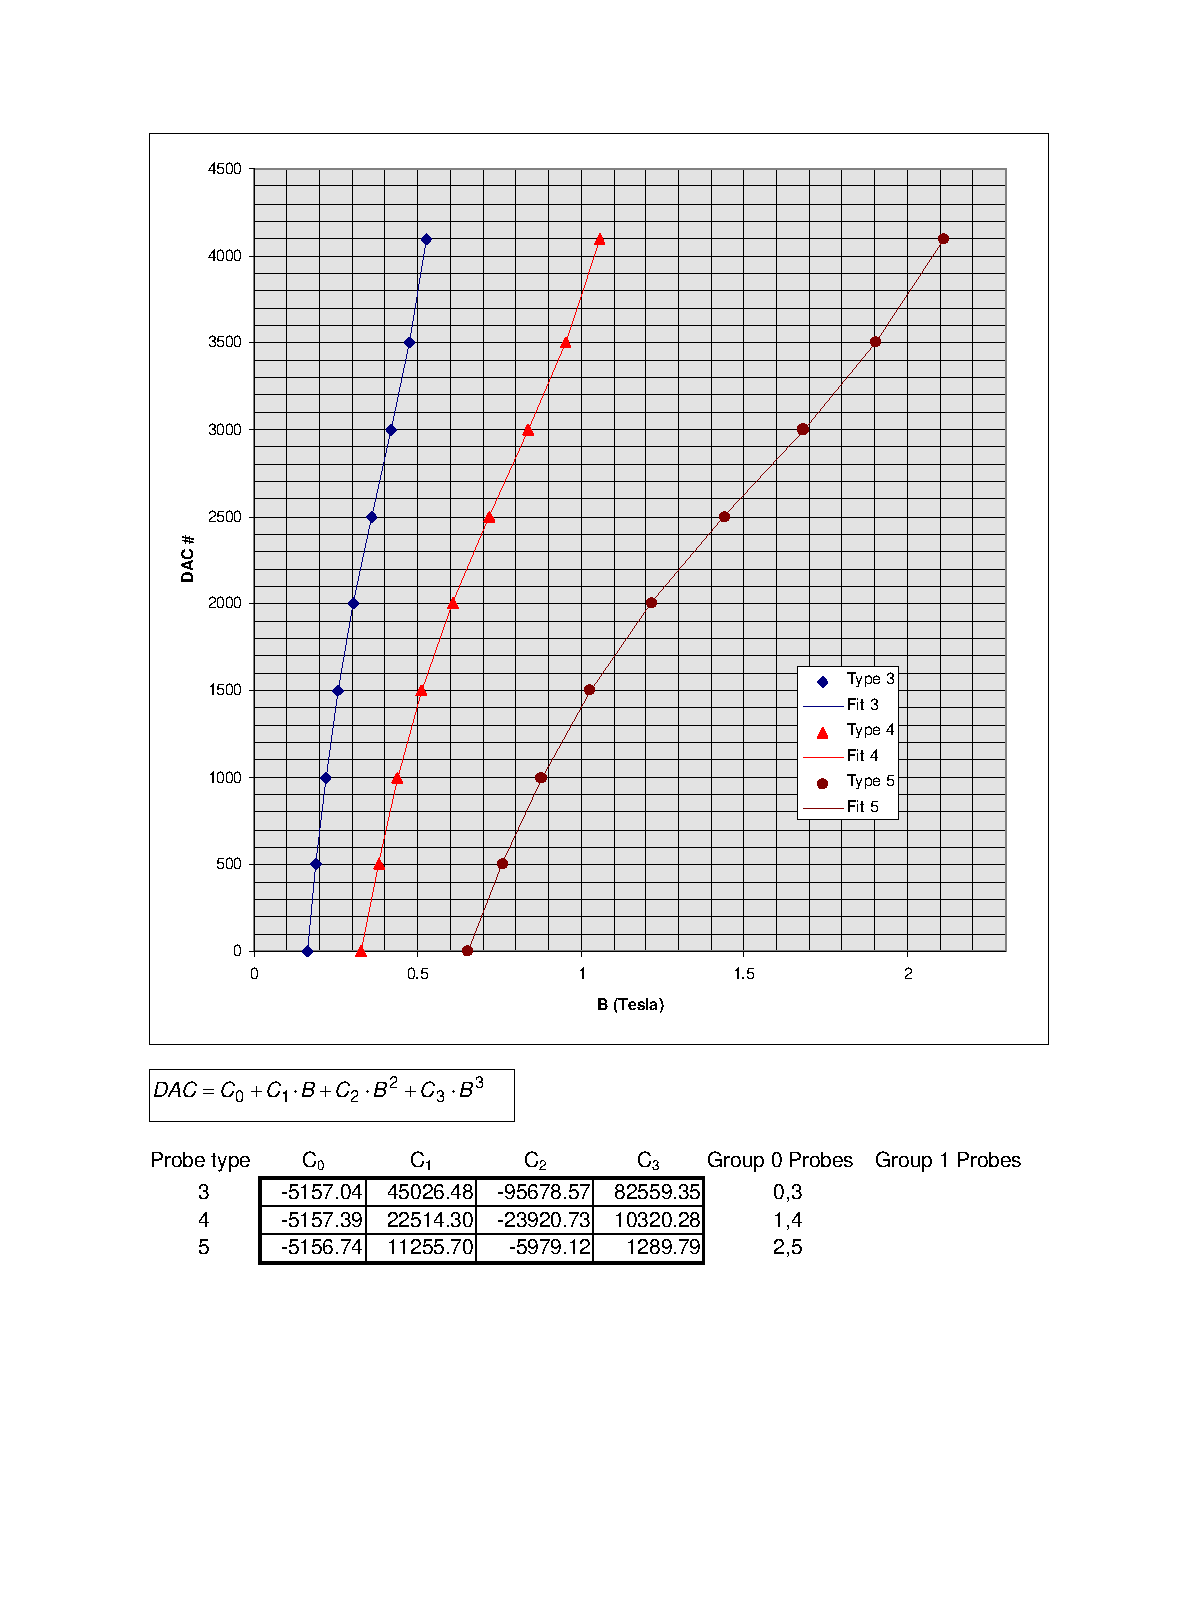
\includegraphics[angle=0,height=20cm,clip]{lerose_fig7}
{\linespread{1.}
\caption[Spectrometers: NMR Probe DAC Calibration]{DAC Calibration for manual operation of NMR probes.}
\label{fig:nmr_dac}}
\end{center}
\end{figure}

The following graphs (see Figures~\ref{fig:nmrcomp4} 
and ~\ref{fig:nmrcomp5}),can be used to determine optimum values for the 
compensating coil control voltage.  It should be noted that the setting 
of the compensating coil current is not very critical in most cases.  In 
general if you're within 10\% of the correct value everything should 
work fine.



\begin{table}
\begin{center}
\begin{tabular}{|cc|} \hline
Probe Type & Field Range (T) \\ \hline 
3 & 0.17 - 0.52 \\
4 & 0.35 - 1.05 \\
5 & 0.70 - 2.10 \\ \hline
\end{tabular}
\caption[Spectrometers: Dipole NMR Probe Field Ranges]{Dipole NMR probe field ranges}
\label{nmr_range}
\end{center}
\end{table}

} %infolev

\infolevtwo{
\subsection{NMR Operating Procedure}

When running in Autopilot mode (see: Simple Spectrometer Field Setting) the 
compensating coil voltage is set automatically and the probe appropriate for 
the field desired is selected. The gaussmeter is placed in SEARCH Mode and the 
dipole power supply software regulator is turned on. In this case the dipole current is 
adjusted to achieve the desired field. The user should just stand 
back and let it work. What follows are instructions for using
the NMR gaussmeter in situations where Autopilot doesn't work or
some special supplemental measurements are required. 

 In principle it is possible to make the field measurements using the 
SEARCH mode in the Teslameter.  In this mode you select a probe and the 
meter explores the whole field range of the probe until it finds and 
"locks" on the resonant signal indicating that it has a field 
measurement.  A ``lock" is indicated on the controls display by an ``L'' to 
the left of the field values.  This has the advantage of simplicity but in practice can 
be time consuming and doesn't always work.  The problem being, in 
situations where there is a lot of noise mixed in with the signal, the 
circuitry has problems distinguishing the signal from the noise and gets 
lost before it ever finds a lock.  The problem is exacerbated when the 
field being measured is at the high end of the probe's range.  In this 
case the search starts at the low end and keeps getting hung up on the 
noise and never gets to the field range of interest.  The solution to 
this problem is to tell the device approximately what field it's looking 
for and use the AUTO mode to find the lock.  In the procedure below that 
is what we will be doing.

In any case, for ``gap probes" (group 0) you must energize and adjust 
the gradient compensating coils for the field ranges to be measured before 
trying to make a measurement.

For studies involving 
10\% changes in the field settings the compensating coil current can be 
set once and left alone.


\noindent\underline{\bf Recommended Procedure:}(turn the {\bf SOFTWARE REGULATOR OFF} for all 
non-autopilot field measurements)\\
For group 0 probes set compensating coils appropriately (see figures).\\
Put the meter in MANUAL mode with SEARCH OFF \\
Select a probe \underline{\bf and} polarity (\underline{\bf Group 0:  
Probes 0, 1, 2 negative; Probes 3, 4, 5 positive}) \\
Type in the appropriate DAC number for the field range being measured (see below) \\
Select AUTO and wait for a lock (indicating a valid field reading) \\
Verify that you have a good lock by checking the oscilloscope for a 
clear resonant signal. \\
If you have problems see the table listing problems and possible 
solutions.

\noindent\underline{\bf Selecting DAC Number}

In selecting the DAC number to use for the field of interest use 
either the graph in Figure~\ref{fig:nmr_dac} or the polynomial at the bottom of the same figure.

\pagebreak
\noindent{\bf Problems and Solutions}\\
\begin{table}[htb]
\begin{tabular}{|p{0.4\textwidth}|p{0.55\textwidth}|}\hline
Symptom & Diagnosis and Cure \\ \hline\hline
Weird numbers on displays, controls for all magnets fouled up 
& Need to reboot.  See instructions below. \\ \hline
NMR Teslameter does not respond to commands and display shows all zeros. 
& Meter's communications are somehow hung up. Push {\bf RESET}. \\ \hline
%Will not lock & Very high noise level makes resonance hard to find. \\
%Still 
Will not lock 
& Very high noise level makes resonance hard to find. Search for the resonance manually by 
  adjusting the DAC in manual mode until you see the resonant signal.  (It helps if you know 
  what field you expect so you'll know where to look). \\ \hline
You find resonance manually but still can't get a lock 
& Check probe polarity. Try decreasing and increasing DAC number by 1. Optimize signal 
  by adjusting compensating coils. \\ \hline
Can't find resonance manually 
& Try a different probe.  Use readings from other probes to tell you where to look for 
 the resonance with the probe that's giving you trouble.  Make sure
 compensating coils are energized properly.  Make sure magnet is on. \\ \hline\hline
\end{tabular}
\caption[NMR: Problems and solutions]{NMR: Problems and solutions}
\label{tab:nmr-problems-solutions}
\end{table}

\begin{table}[ht]
\begin{center}
\begin{tabular}{|p{0.3\textwidth}|p{0.3\textwidth}|p{0.3\textwidth}|}\hline
Problems & Explanation & Action \\ \hline
NMR not locked but current is changing in the right direction 
& Normal operation for large field changes  
& Wait. (see above) \\ \hline
NMR locked but current going in the wrong direction.
& Normal operation. 
& Wait. \\ \hline
NMR locked but field not correct and current not changing 
& Field regulation is disabled or software is confused.
& Check that field regulation is enabled. Enter desired field value or one
  very near the desired value again. \\ \hline
NMR field display freezes. (Usually but not always shows  -\#.0000000)
& NMR Gaussmeter is not communicating with software.
& Push {\bf RESET}. \\ \hline
\end{tabular}
\end{center}
\caption[NMR troubleshhoting]{NMR troubleshooting
}
\label{tab:hrs_nmr_2}
\end{table}

} %infolev

\begin{safetyen}{10}{15}
\subsection{Authorized Personnel}
\end{safetyen}

The individuals shown in Table \ref{tab:nmr:personnel} are responsible for NMR operation problems.

\begin{namestab}{tab:nmr:personnel}{NMR: authorized personnel}{%
      NMR: authorized personnel.}
  \JavierGomez{\em Contact}
  \JohnLeRose{}
\end{namestab}



\newpage
\section[Collimators and Sieve Slits]{Collimators and Sieve Slits
\footnote{
  $CVS~revision~ $Id: slit.tex,v 1.5 2003/12/13 06:23:38 gen Exp $ $ 
}
\footnote{Authors: J.LeRose \email{lerose@jlab.org}}
}

Both spectrometers have front-end devices for calibrating the optical
properties of the spectrometers. These are known as the collimator boxes.
These boxes are positioned between the scattering chamber and the 
first quadrupoles (Q1). Each box is carefully aligned and rigidly attached
to the  entrance flange of the Q1 of the respective spectrometer.  The boxes are
part of the vacuum system of the spectrometer.
In the septum configuration sieve slits and collimators are installed and removed manually.

Inside each box a ladder is mounted which is guided by a linear bearing
and moved up and down by a ball screw. On this ladder 3 positions are 
available to insert collimators. Below this ladder
a special valve is mounted that can isolate the vacuum in the spectrometer
from the target system. This valve should be activated when it is moved
in front of the holes connecting the box with spectrometer and target chamber.
\infolevone{
A schematic view of the collimator box is shown in Fig.~\ref{fig:coll}.

\begin{figure}
\begin{center}
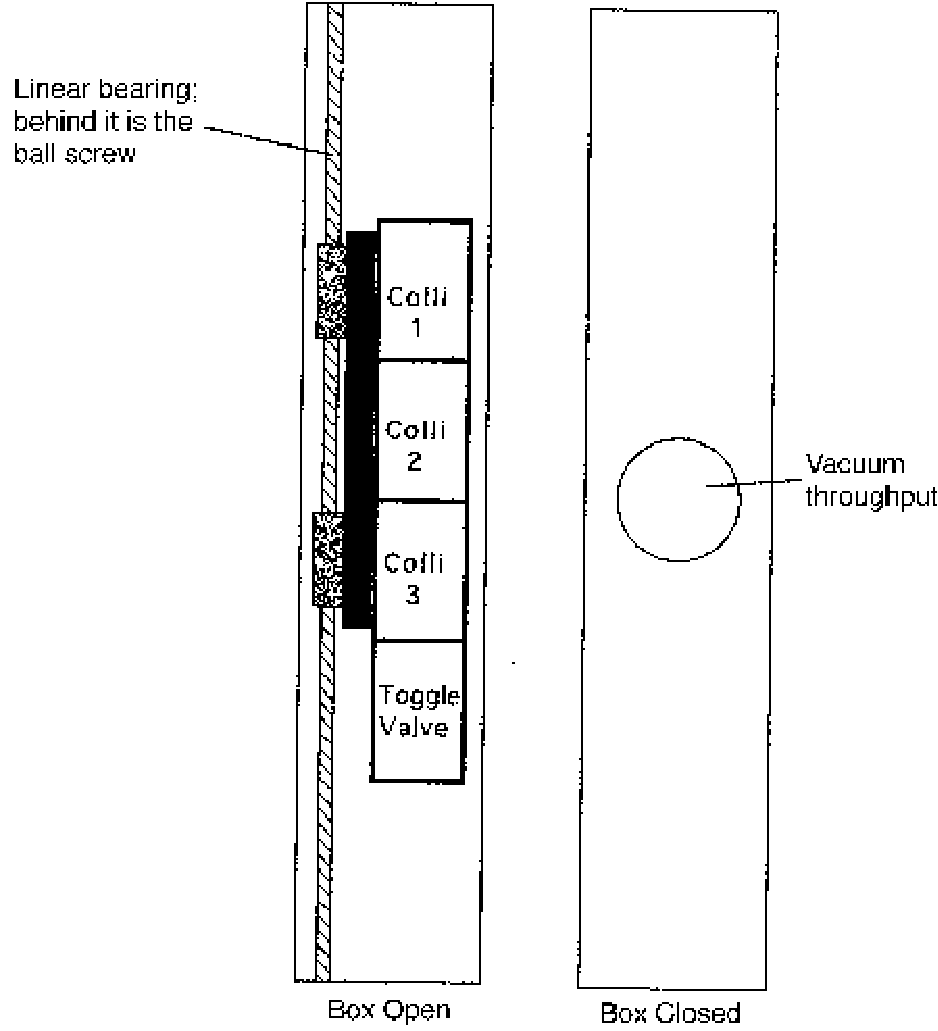
\includegraphics[angle=0,width=13cm,clip]{collimator_clip}
{\linespread{1.}
\caption[Spectrometers: Collimator Box Schematic]{Schematic layout of the collimator box.}
\label{fig:coll}}
\end{center}
\end{figure}
} %infolev

Vacuum requirement is $10^{-6}$ Torr. The material for the box is 
aluminum. It is possible to open one side of the box so that
collimators can be exchanged. The
reproducibility of collimator positions after moving
the ladder and/or after replacing a collimator is
better than 0.1 mm in horizontal and vertical direction.
The dimensions of the box are
roughly height=175 cm , width=35 cm and depth=15 cm.
The tolerance in the dimension
of the 7 msr collimator hole is $\pm0.5$ mm in each direction. 
The tolerance in the position
of each of the sieve-slit holes is $\pm0.1$ mm in each direction.

\infolevone{
\begin{figure}
\begin{center}
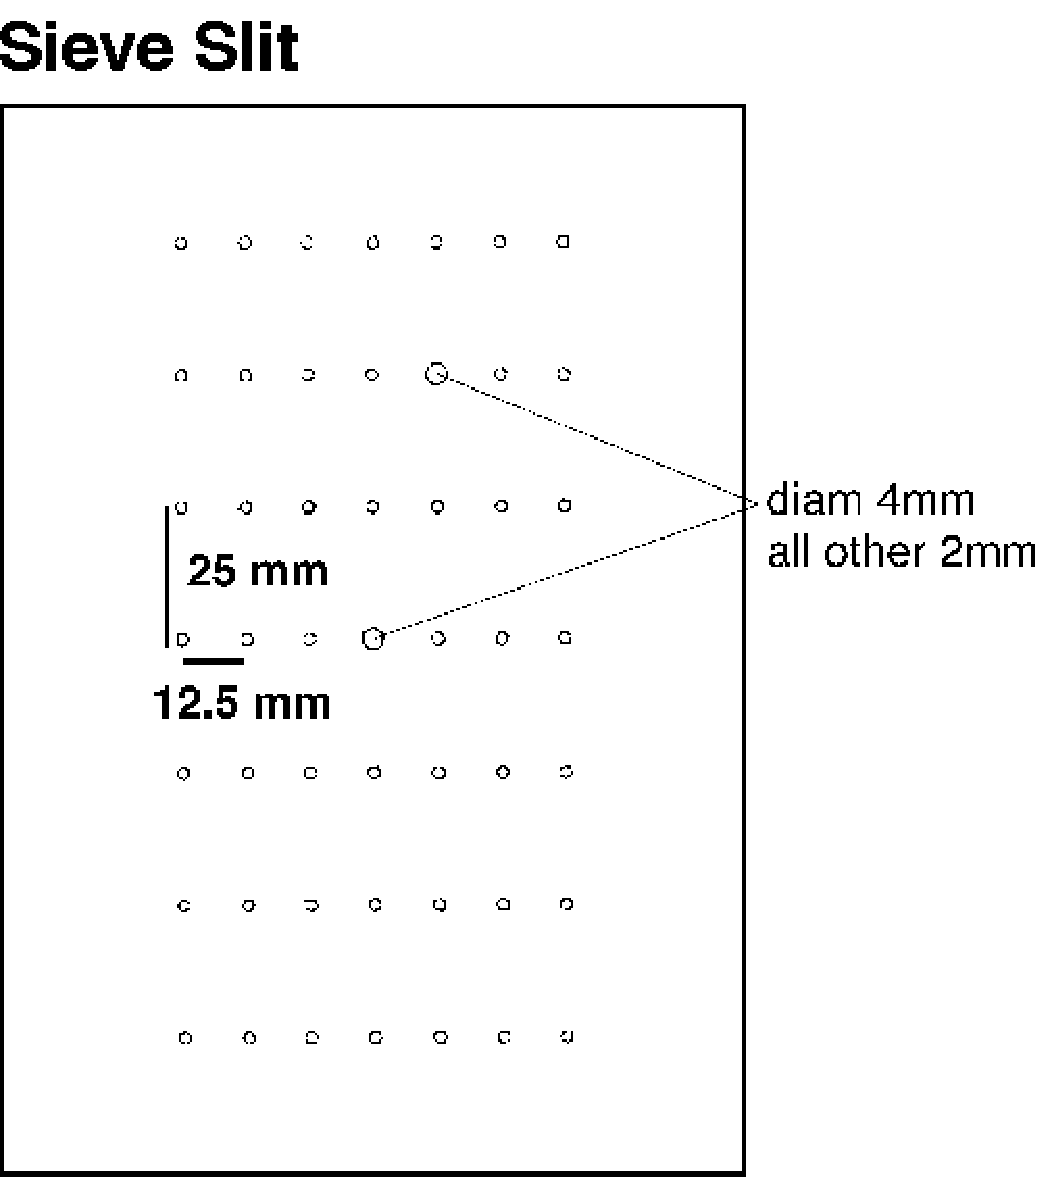
\includegraphics[angle=0,width=13cm,clip]{sieveslit}
{\linespread{1.}
\caption[Spectrometers: Sieve Slit]{Sieve slit collimator for optics calibration.}
\label{fig:sieve}}
\end{center}
\end{figure}
} %infolev
A typical sieve slit collimator 
\infolevone{(shown in Fig.~\ref{fig:sieve})
} %infolev 
consists of a plate of roughly 14 cm x 20 cm containing 49 holes
positioned in a regular 7x7 pattern. This slit is made out of 5
mm thick tungsten.
The holes have a diameter of 2 mm except for the central one and one positioned
off-diagonal which have a diameter of 4 mm. The horizontal distance between the
holes is 12.5 mm while the vertical distance is 25.0 mm.
%
%To get the latest information on the dimensions and locations of the collimators see 
%the Hall A homepage on the web%
%\htmladdnormallinkfoot{}{\url{
%http://hallaweb.jlab.org/
%}}.

To get the latest information on the dimensions and locations of the collimators see 
the Hall A homepage on the web%
\htmladdnormallinkfoot{}{\url{
http://hallaweb.jlab.org/
}}.

\begin{safetyen}{10}{15}
\subsection{Safety Assessment}

The collimator boxes form part of the vacuum system for each spectrometer. All hazards
identified in section spectrometer vacuum section applies to the collimator box as well.

In addition, safe access to the top of
the collimator boxes is needed  during manual operation of the box as outlined below.
Due to the proximity of the collimator boxes to the scattering chamber, and Q1 quadrupoles,
all necessary safety precautions with regards to vacuum windows, electrical power cables, 
cryogenic transfer lines, and high magnetic field should be taken. The same precautions also apply 
to the collimators and sieves in the septum configuration. In that case the sieve and collomators
can be considered part of the beamline. A survey and
appropriate RADCON designated proceedures must be followed when dealing with septum sieves 
and collimators.
\end{safetyen}

\infolevtwo{
\subsection{Operating Procedure}
Slit position is changed remotely from the standard Hall A control screen.
In the case of a spectrometer configuration involving the septum magnets collimators and sieves are
changed manually in the Hall.
} %infolev

\subsection{Authorized  Personnel} 

\begin{itemize} 
\item[~]E. Folts - x7857 (mechanical and vacuum systems).
\item[~]J. Gomez - x7498 (computer controls and electrical systems).
\end{itemize} 

% ===========  CVS info
% $Header: /group/halla/analysis/cvs/tex/osp/src/hrs/slit.tex,v 1.5 2003/12/13 06:23:38 gen Exp $
% $Id: slit.tex,v 1.5 2003/12/13 06:23:38 gen Exp $
% $Author: gen $
% $Date: 2003/12/13 06:23:38 $
% $Name:  $
% $Locker:  $
% $Log: slit.tex,v $
% Revision 1.5  2003/12/13 06:23:38  gen
% Septum added. Name tables. Polishing
%
% Revision 1.4  2003/12/05 06:49:07  gen
% infolevels added, polishing
%
% Revision 1.3  2003/06/06 16:13:37  gen
% Revision printout changed
%
% Revision 1.2  2003/06/05 23:30:00  gen
% Revision ID is printed in TeX
%
% Revision 1.1.1.1  2003/06/05 17:28:31  gen
% Imported from /home/gen/tex/OSP
%
%  Revision parameters to appear on the output

\newpage
\infolevtwo{
\section[Spectrometer Alignment]{Spectrometer Alignment
\footnote{
  $CVS~revision~ $Id: AlignmentOps.tex,v 1.8 2003/12/17 03:59:48 gen Exp $ $ 
}
\footnote{Authors: J.Gomez \email{gomez@jlab.org}}
}

At present, the systems implemented to determine the alignment of each spectrometer
(roll, vertical angle/pointing and horizontal angle/pointing) without the help of the
Accelerator Division Survey group are limited to roll, vertical angle and horizontal angle.
All alignment information is displayed in the ``ALIGNMENT'' mosaic of the ``Hall A
General Tools'' EDM screen%
\infolevtwo{ (see Fig.~\ref{fig:medm-hlamain-tools})}
(``EOS Menu'' $-->$ ``EDM (HLA Main)'' $-->$ ``Hall A Main Menu'' $-->$ ``Tools'').

A bi-axial inclinometer is used to determine the roll and vertical angle (also known as pitch)
of each spectrometer. These inclinometers are attached to the back of the dipoles at the power
supply platform level. The raw inclinometer measurements, in Volts,
are displayed as ``Tilt X'' and ``Tilt Y''. The inclinometer temperature is also given
(`` Tilt T''), in degree Celsius. From these values, the ``ROLL'' and ``PITCH'' values are
calculated.
Agreement between the inclinometer readings and survey measurements
are better than $\pm$ 0.1 mrad over all presently available history.

The horizontal spectrometer angle is determined from floor marks set in
place by the survey group. Floor marks have been placed every 0.5 $^\circ$ covering the useful range of
both spectrometers.
There are two concentric rings of floor marks in the hall. We will concentrate in the
inner ring which covers the angular range of both spectrometers. The outer ring is
similar.
The inner-ring floor marks are located at a distance of $\sim$10 $m$ from the target center.
A ruler attached to each spectrometer dipole runs over the floor marks and it acts as a vernier to interpolate
between marks. The location of a given floor mark on the ruler can be viewed from the Hall A Counting
House through a TV camera (labeled ``Front Camera'') .
The camera is able to move along the length of the ruler so that any
parallax effect can be eliminated. The camera motion is controlled from the ``Tools'' screen
through two push buttons (``FRONT CAMERA'' - ``MOVE +'' and ``MOVE --'').
Two fields in the ``ALIGNMENT'' mosaic
(``Flr Mrk'' and ``Vernier'') allow to input
the values read from the TV monitor. The effective spectrometer angle is then calculated and displayed
as ``Angle''. The application ``HRS Floor Marks'' calculates the floor mark and vernier value
to which the spectrometer should be set
to obtain a given angle. Spectrometer horizontal angle surveys and floor mark determinations
agree to $\pm$ 0.2 mrad.

\newpage
\begin{safetyen}{10}{15}
\subsection{Authorized  Personnel} 
\end{safetyen}
The authorized personnel is shown in table \ref{tab:align:personnel}.
\begin{namestab}{tab:align:personnel}{HRS alignment: authorized personnel}{%
      HRS alignment: authorized personnel.}
  \JessieButler{\em Contact}
\end{namestab}

} %infolev


% ===========  CVS info
% $Header: /group/halla/analysis/cvs/tex/osp/src/hrs/all.tex,v 1.3 2003/06/06 15:44:08 gen Exp $
% $Id: all.tex,v 1.3 2003/06/06 15:44:08 gen Exp $
% $Author: gen $
% $Date: 2003/06/06 15:44:08 $
% $Name:  $
% $Locker:  $
% $Log: all.tex,v $
% Revision 1.3  2003/06/06 15:44:08  gen
% Revision printout changed
%
% Revision 1.2  2003/06/05 23:30:00  gen
% Revision ID is printed in TeX
%
% Revision 1.1.1.1  2003/06/05 17:28:31  gen
% Imported from /home/gen/tex/OSP
%
%  Revision parameters to appear on the output

\chapter{High Resolution Spectrometers (HRS)}
\graphicspath{{hrs/figs/}}
\renewcommand{\dirfig}[0]{hrs/figs}
\renewcommand{\dircur}[0]{hrs}

\infolevone{
\chapter[High Resolution Spectrometers (HRS)]{High Resolution Spectrometers (HRS)
}
\footnote{Authors: J.LeRose \email{lerose@jlab.org}}
}
\label{chap:hrs}

\infolevone{
\section{Overview}
   
The Hall A spectrometers and associated instrumentation are designed to 
perform high resolution and high accuracy experiments.  The goal is to 
achieve a missing mass resolution of $\sim$ 200-500 keV to clearly 
identify the nuclear final state.  An absolute accuracy of $\sim$ 1\% is 
also required by the physics program planned in the Hall, which implies 
$\sim$ 10$^{-4}$ accuracy in the determination of particle momenta and 
$\sim$ 0.1 mr in the knowledge of the scattering angle.

The instruments needed are a high resolution electron spectrometer 
(HRES) and a high resolution hadron spectrometer (HRHS), both with a 
large angular and momentum acceptance.

\begin{figure}[tbp]
\begin{center}
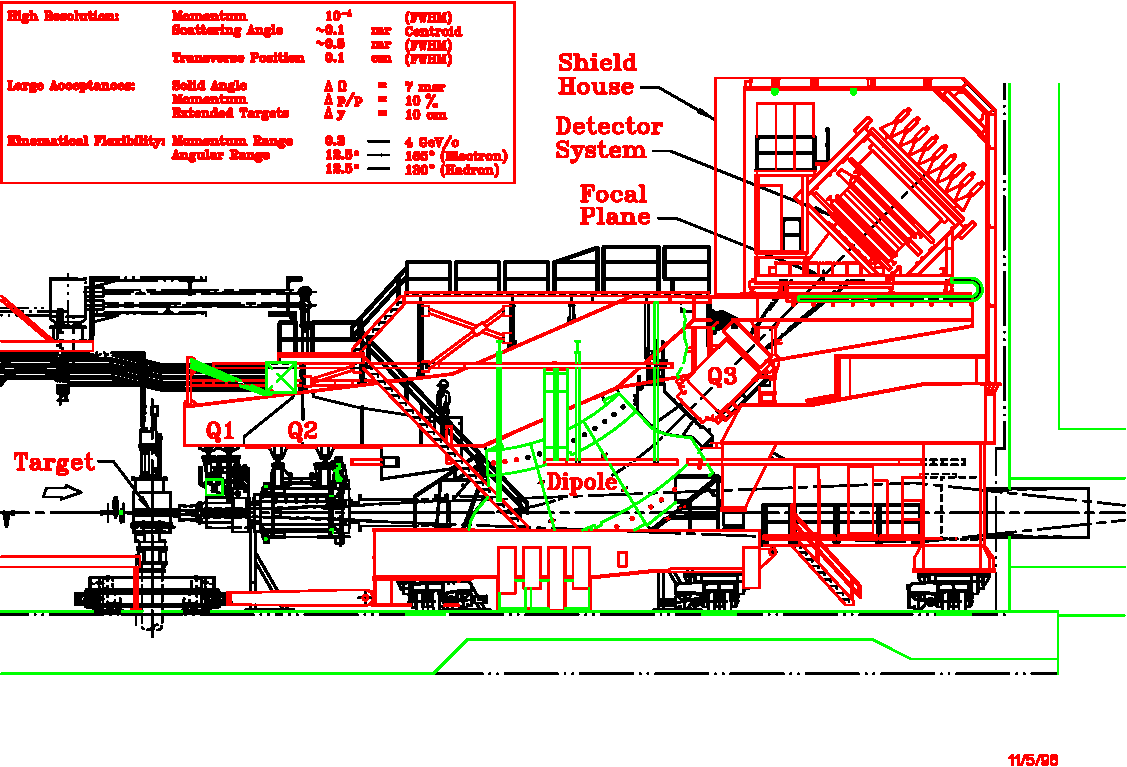
\includegraphics[angle=0,width=0.9\textwidth,clip]{figure0101_r}
\caption[Spectrometers: Elevation View of Hall~A HRS]{A side view of the Hall~A
HRS spectrometer.}  
\label{fig:hrs_ev}
\end{center}
\end{figure}
 
\begin{figure}[tbp]
\begin{center}
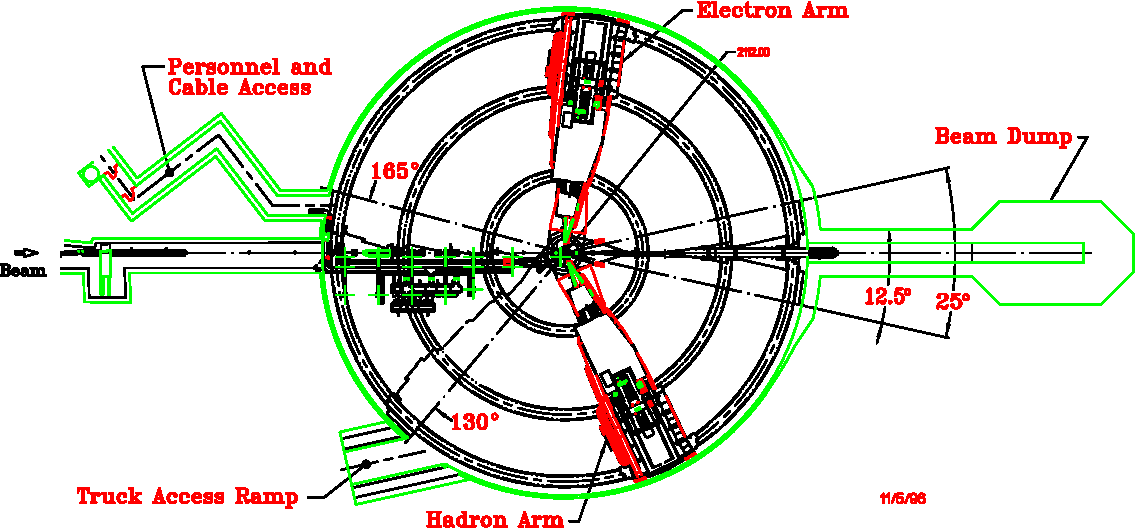
\includegraphics[angle=0,width=0.9\textwidth,clip]{figure0102_r}
\caption[Spectrometers: Plan View of Hall~A]{A bird's eye view of the Hall~A
end-station at TJNAF.}  
\label{fig:hrs_pv}
\end{center}
\end{figure}


A layout of the 4 GeV/c High Resolution Electron Spectrometer is shown 
on Figures~\ref{fig:hrs_pv} and \ref{fig:hrs_ev}.
Its main design characteristics are 
given in the attached table.  The spectrometer has a vertical bending 
plane and 45$^{\circ}$ bending angle.  The QQDQ design includes four 
independent superconducting magnets, three current-dominated 
cos2$\theta $ quadrupoles and one iron-dominated dipole with 
superconducting racetrack coils.  The second and third quadrupoles of 
each spectrometer have sufficiently similar field requirements that they 
are of identical design and construction.  The overall optical length, 
from target to focal plane, is 23.4 m.  Optically, the HRHS 
is essentially identical to HRES. In fact the two spectrometers can be used 
interchangeably to detect either positively or negatively charged particles 
as needed by any particular experiment. They are now commonly refered to 
as ``The Left Arm'' and ``The Right Arms'' rather than ``Hadron'' and ``Electron'' 

The support structure includes all system elements which bear the weight 
of the various spectrometer components and preserve their spatial 
relationship as required for 45$^{\circ}$ vertical bending optics.

The alignment and positioning system includes all the elements which 
measure and adjust the spatial relationship.  The support structure 
consists of the fabricated steel components which support the magnets, 
detector, shield house and associated equipment.  It is composed of the 
box beam, which supports the outer elements in fixed relative position 
atop the dipole; the dipole support bracket, upon which the dipole rests on 
the jacks; the cradle, upon which the dipole rests through the vertical 
positioning system, VPS; and a portion of the shield house load through 
the inboard legs of the gantry; the gantry, which supports the shield 
house and the magnet power supplies; and the bogies, which support the 
cradle-gantry assembly and roll on the floor plates and provide the 
driving power to move the two spectrometer arms.

The detector package (described in detail in Chapter \ref{chap:hrs-det})
is supported on the box beam and is surrounded by 
the shield house.  It must perform two functions, tracking and particle 
identification, PID.  The most important capability of focusing 
spectrometers is measuring precisely the momenta and entrance 
orientations of the tracks.  Momentum resolution of 10$^{-4}$ is 
obtainable, consistent with the resolution of the incident beam.

The actual configuration of the detector package varies from experiment to
experiment. The description given here is only an example of what is possible.
}

\infolevone{
A particle traversing the detector stack 
(Figure~\ref{fig:hrs_electron_det}) encounters two sets of horizontally
mounted, vertical drift wire chambers (x,y) with two planes of 368
wires in each chamber. The track resolution is $\sim$ 100 $\mu$m.  
From the chamber information both 
positions and angles in the dispersive and transverse directions can be 
determined.  The information from these chambers is the principal input 
of the tracking algorithms.

The chambers are followed by a scintillator hodoscope plane designated S1. 
This plastic scintillator array provides the timing reference for 
the drift chambers, and is also used in trigger formation and in combination 
with a second hodoscope pair it can provide time of flight particle 
identification.  These scintillators can also be used to perform crude 
tracking.

The next element encountered by a particle is a gas threshold \Cherenkov{} 
detector.  This is used for particle identification.  This gas threshold \Cherenkov{} detector can be swapped 
against an Aerogel detector, with a similar function.

The second hodoscope plane, S2, is located directly behind the 
gas \Cherenkov{}.  Its function is essentially the same as that of S1.  
In the hadron spectrometer an option exists to have this hodoscope 
pair be preceded by a third chamber, to improve tracking.
 Each of the two spectrometers 
have gas and Aerogel \Cherenkov{} detectors which can be used
 when they are in electron detection mode.

The final elements in the detector stack on HRSE are 
the pre-shower and the total-absorber lead glass shower 
calorimeter.  This is used for energy determination and PID.

\begin{figure}[tbp]
\begin{center}
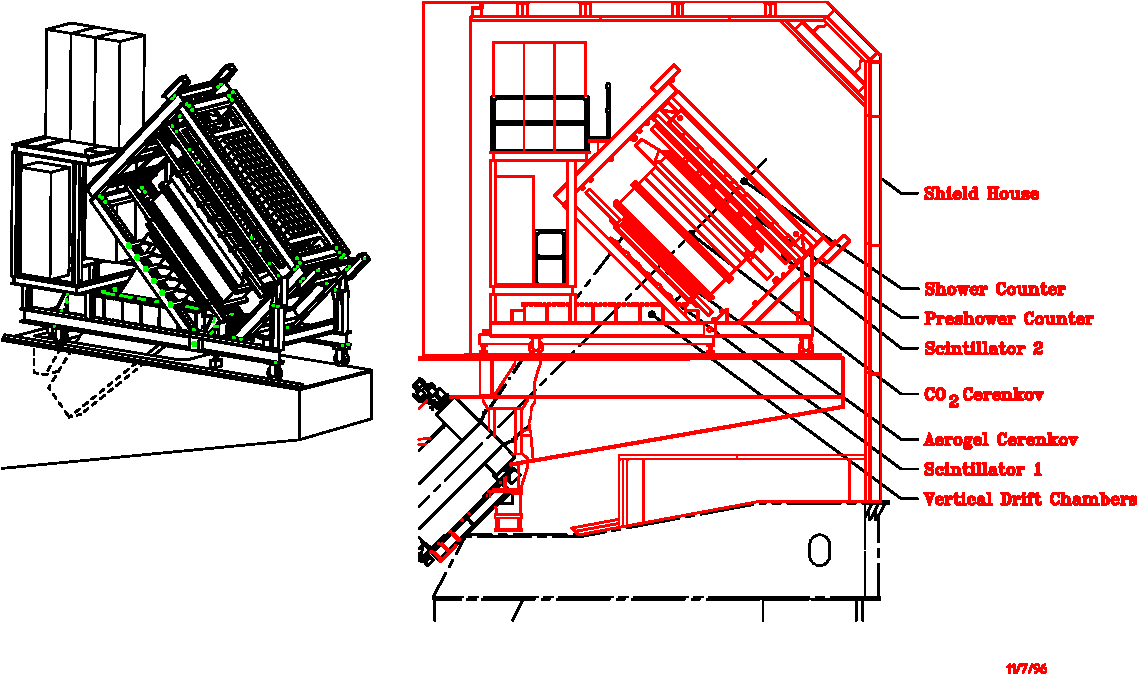
\includegraphics[angle=0,width=\textwidth,clip]{figure0103_r}
{\linespread{1.}
\caption[Spectrometers: Electron Arm Detectors]{The electron spectrometer detector stack.}
\label{fig:hrs_electron_det}}
\end{center}
\end{figure}

\begin{figure}[tbp]
\begin{center}
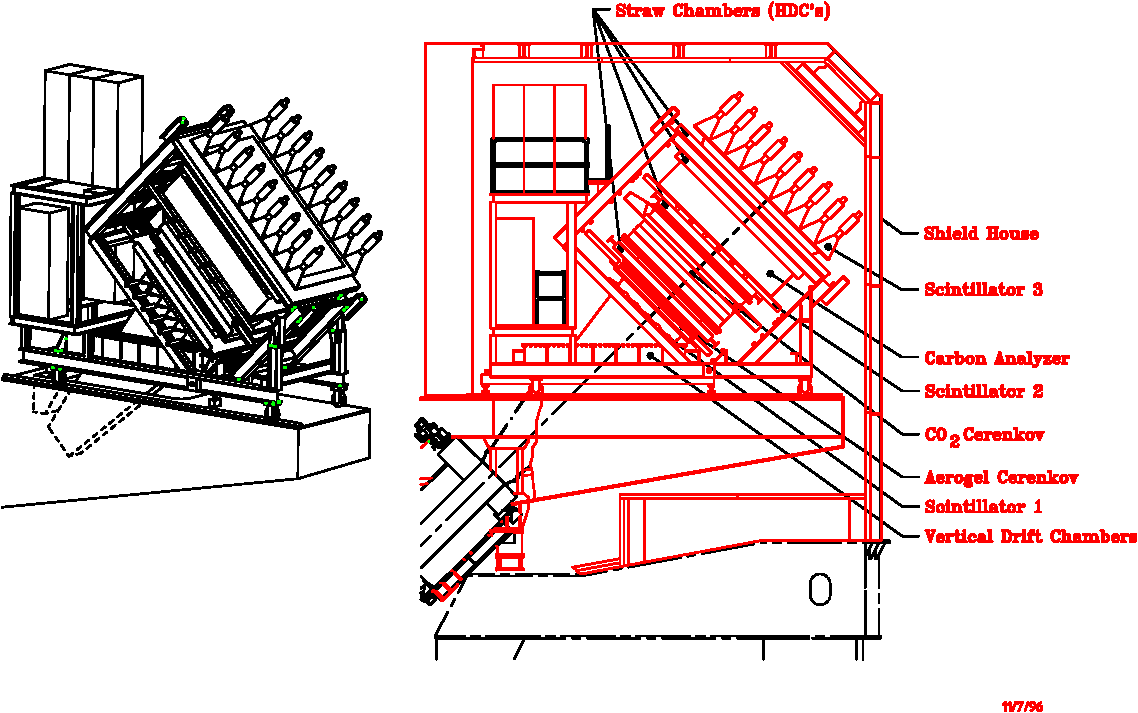
\includegraphics[angle=0,width=\textwidth,clip]{figure0104_r}
{\linespread{1.}
\caption[Spectrometers: Hadron Arm Detectors]{The hadron spectrometer detector stack.}
\label{fig:hrs_hadron_det}}
\end{center}
\end{figure}


The hadron detector is shown schematically in 
Figure~\ref{fig:hrs_hadron_det}.  It consists 
of two sets of (x,y) vertical drift wire chambers identical to those of the 
electron arm.  The remaining part of the detection system is used to 
define the level 1 trigger, as well as for particle identification and 
timing.  It consists of two minimally segmented planes of 
scintillation counters equipped with photomultipliers at both ends, and 
it includes \Cherenkov{} counters (gas CO$_2$ and Aerogel).

In addition, a proton polarimeter is installed in the back of the 
detector package to measure the polarization of the proton using a 
segmented carbon analyzer up to 60 cm in thickness to allow measurements 
over a wide range of proton energies.  A pair of front and a pair of 
rear straw tube wire chambers determine the incident and 
scattered angles, respectively.  The 
polarimeter detectors are dimensioned to accept a 20$^{\circ}$ cone of 
scattered protons.

Several support systems are necessary in addition to the basic 
components mentioned above.  They include gas supply systems for the 
wire chambers, high voltage supplies, readout electronics, a second 
level trigger, software for data analysis and testing, and a remotely 
controllable mechanical system.

For each spectrometer, all detectors are mounted on a 
single rigid support frame along with their associated electronics.  The trigger electronics are located on the support frame, next to the detectors.

To reduce the resolution degrading effects of multiple scattering, the 
entire interior of the spectrometer from the collimator box to the detector hut 
is a vacuum vessel.  The ends of this evacuated volume are capped by 
relatively thin vacuum windows.
}

\begin{safetyen}{0}{0}
\section{High Resolution Spectrometers}
\label{sec:hrs-safety}
\end{safetyen}

The principle concern with the spectrometers is that they are large, 
and have associated vacuum, hydraulic, cryogenic and magnet systems all of 
which can be potentially dangerous.

The bogies which move the massive 1200 ton spectrometers must be 
carefully operated.  Inspection of the floor and wheels to ensure there is no 
debris which the wheels could ride over is mandatory.  Similarly 
personnel need to be aware that the spectrometers are moving so that no one 
inadvertently gets trapped.

The vacuum systems associated with the spectrometers are essentially 
pressure vessels (see Chapter \ref{chap:vacuum} for more details).
Care should be exercised so as not to puncture the 
windows.

The magnets themselves are installed inside cryostats.  These vessels 
are exposed to high pressures and are therefore equipped with safety 
relief valves and burst discs.

The hydraulic system originally intended to operate the vertical positioning system (VPS) 
and the horizontal positioning system (HPS) has effectively been dismantled, after problems were encountered during the initial attempted operation of the system.

The cryogenic system operates at elevated pressure at 4K.  One must 
guard against cold burns and take the normal precautions with pressure 
vessels when operating this system.  Only authorized personnel are permitted to install 
and take out U tubes.

The magnets have a great deal of stored energy as they are large 
inductors. Always make sure people are clear of them and that
the dump resistor is attached to the magnet.

There are several major safety concerns with regards to the detectors, 
namely 1) flammable gas located in the VDC, 2) ODH hazard due to 
CO$_2$ in the \Cherenkov{} counter, 3) high voltage due to the photo 
multipliers on the various detectors and 4) a thin vacuum window 
separating the detector array from the vacuum system in the 
spectrometers.

\infolevltone{
\begin{safetyen}{5}{10}
For more information consult the full OSP manual~\cite{HallAosp}.
\end{safetyen}
} %infolev

\begin{safetyen}{10}{15}
\subsection{Authorized Personnel}
\end{safetyen}

In the event that problems arise during 
operation of the magnets, qualified personnel should be notified
(see Table \ref{tab:hrs:personnel}).  
This includes any prolonged or serious problem with the source of magnet 
cryogens (the ESR).  On weekends and after hours there will be a 
designated individual on call for magnet services.  Any member of the 
Hall A technical staff is qualified to deal with unusual magnet 
situations but in the event of serious problems the technician on
call should be contacted.

\begin{namestab}{tab:hrs:personnel}{HRS: authorized personnel}{%
      HRS: authorized personnel. ''W.B'' stands for the white board 
      in the counting house.}
   \TechonCall{\em Contact}
   \EdFolts{}
   \JackSegal{}
   \HeidiFansler{}
   \JessieButler{}
   \AndrewLumanog{}
   \JasonGlorioso{}
   \MahlonLong{}
\end{namestab}

\infolevone{
\section{The Magnets of HRS}

Each HRS is composed of three superconducting quadrupole magnets, Q1, Q2, 
and Q3, and one superconducting dipole magnet.  The large quadrupoles were 
manufactured for JLab by SIEMENS, the small quadrupole by SACLAY, while 
the dipole was built for JLab by WANG NMR.  The quadrupole magnets are 
referred to as Q1, Q2, and Q3, where a particle first traverses Q1, then 
Q2 and the dipole magnet and finally traverses Q3.

The magnet system is followed by a large steel and concrete detector 
hut, in which all detector elements reside.  Most of the 
detector elements have been built by universities involved in the Hall A 
physics program.

The HRS magnet system is the cornerstone of the Hall A activities.  
Many of the experiments approved in Hall A center on physics at high 
resolution and other short-range phenomena, and rely on a spectrometer 
able to momentum analyze charged particles up to very high momenta.  The 
design value for the maximum momentum accessible to the HRS magnet 
system is 4 GeV/c.
}

\subsection{Magnets and Power Supplies}

\infolevone{
The HRS magnet's are all superconducting and hence their coils must be 
maintained at cryogenic temperatures during operations.  The LHe 
required by the magnets is supplied by the End Station Refrigerator, ESR.

All the HRS magnets cryogenic services are supplied through the overhead 
cryogenic lines.  The distribution network begins at the distribution 
box over the pivot.  This box is connected to the rest of the network 
via the flexible transfer lines over the pivot.  The network is adjacent 
to the upstairs catwalk of the HRS.

Cryogenic information about each magnet is available on the control 
screens in the counting house, one for each magnet.  Normally during run 
periods the control screens are sent upstairs to the Hall A counting 
house and information on all the HRS magnets is available on the HRS 
control screen located in the center of the main console.  The control 
of all magnets is described in a following Section.

The power supplies for the magnets are located on the gantry balcony 
adjacent to the magnets.  The supplies are all cooled with low conductivity water (LCW).
}

\begin{safetyen}{10}{15}

Under no 
circumstances should any panel of any magnet power supply be opened by someone 
other than authorized personnel.  There are also 
signs posted listing the dangers of high magnetic fields.
\end{safetyen}

\infolevone{
A control interface for the power supplies is available through the 
HRS control screen in the Hall A counting house.
}

\infolevone{
\subsection{Quadrupole Magnets}

The quadrupoles provide some of the 
focusing properties of the spectrometer and to a large extent 
its acceptance.  Operating limits imposed on the 
quads are as follows: 1850A for Q2 and Q3 and 3250A 
for Q1.

All three quadrupoles for the HRS spectrometer are warm iron 
superconducting magnets.  The soft iron around the superconducting coil 
enhances the field at the coil center and reduces stray fields.  The 
basic parameters for the first quadrupole, Q1, are an effective length of about 
0.9 $m$, useful aperture of 0.3 $m$ and a field gradient of 9.5 
T/m.  To achieve the lowest possible angle setting of the HRS 
spectrometer (with respect to the beam line) the incident electron beam passes through
a notch in the outer yoke of Q1 when the spectrometer is at
its smallest angle of 12.5$^\circ$ . The 
other two quadrupoles, Q2 and Q3, are essentially identical with an 
effective (magnetic) length of about 1.8 meter, a useful aperture of 
0.6 $m$ and a field gradient of 3.5 T/m.
}

\infolevthree{
The maximum operating currents (assuming a 4 GeV/c momentum particle) 
for the quadrupoles are about 3000 A, 1700 A, and 1600 A, for Q1, Q2, and 
Q3, respectively.  This will render pole field values 
of 1.2, 1.0, and 1.0 T, respectively.  The energy stored in the 
quadrupole fields is sufficient to cause an unrecoverable quench if all 
the energy stored is dumped into the magnets.  Therefore a quench 
protection circuit is incorporated.  However, a quench can only happen 
if the cryomagnets have a helium level below the coil 60\% during operation.

The operating current to the Q1 quadrupole coils is provided by Danfysik 
System 8000 power supplies, which can operate up to 3500 A current and 5 
V.  The power supplies will be cooled with a combined maximum 
water flow of 45 liters per minute.

In addition to the main quadrupole windings, all quadrupoles have 
multipole windings.  To further optimize focusing properties of the HRS 
magnet system, it was intended to operate including some of these multipole 
trim coils in order to reduce higher order aberrations.
The operating current for these multipole corrections would be 
small, only (the multipole corrections are typically less than 2\% of 
the main quadrupole field), of order 50 A. Since the sextupoles were inadvertently 
installed rotated 90 $^\circ$ from their correct
orientation, these trim coils are now considered useless 
and there are at present no plans to use them.

\subsection{Cryogenic Procedures}

The cryogenics control is handled by the JLab Cryogenics Group.  The cryo control coordinator 
can be reached at the CHL (x7405) or by calling the MCC.

\subsection{First Time Startup Check List.}  

See attached check lists for all quadrupole and dipole magnets
 (Tables~\ref{tab:dip_check}, \ref{tab:q1_check}, and \ref{tab:q23_check}).
} %infolev

\infolevone{
\subsection{Dipole Magnet}

The dipole, by virtue of its field index, provides both
dispersion and focusing.  The present operations envelope 
states that the supply for the left HRS dipole may not be
operated at a current above 1800 A (4.4 GeV/c). The supply for the right HRS
dipole may not be operated above 1200 A (3.2 GeV/c), due to complications
caused by an internal short. 

The dipole for the HRS spectrometer is a superconducting, cryostable 
magnet.  Its basic parameters are an effective length of about 6.6 $m$, a 
bend radius of 8.4 $m$, and a gap width of 25 $cm$.  It is configured to 
achieve a 45 degree bending angle for 4 GeV/c momentum particles at a 
central field excitation of 1.6 T.  For the HRS dipole to reach 1.6 T 
an operating current of about 1500 A is required.
} %infolev

\infolevthree{
The dipole has been designed to achieve cryostability up to a field of 2 
T, and this property has been extensively tested up to a field of 1.6 T. 
 The cryostable coils are equipped with an energy removal circuit to 
cover the possibility of an unrecoverable quench.  However, this can 
only happen if the helium level drops below the coil during operation.  
The current to the coils will be provided by a Dynapower Corporation power 
supply, which can operate up to 2000 A and 10 V.  This 
power supply is located on the gantry beside the dipole, and will be 
cooled with a maximum water flow of 35 liters per minute.
The total water flow needed to cool the 4 power 
supplies for the HRS magnet system (dipole and quadrupoles) amounts to 
80 liters per minute, with a supply pressure of cooling water for Hall A 
of 100 psi.
} %infolev

\infolevtwo{
\section{Operation of the HRS Magnets}

\subsection{Introduction}

This is an abbreviated operating manual for 
the HRS superconducting magnets specifically designed for Hall A 
experimenters.  It provides instructions for setting currents, invoking 
NMR field regulation and general system monitoring.  Curious readers are 
directed to the references for more in-depth operating instructions and 
other technical manuals. Copies of the following supporting
documents are available in the Hall A Control Room and through the Hall A webpage
(see Table~\ref{tab:hrs-mag-manuals}).

\begin{table}[htp]
\begin{center}
\begin{tabular}{|l|l|}
\hline
References & \\
\hline 
WANG NMR Dipole & User Manual \\
Dynapower & Instruction Manual \\
Appendix & NMR Tesla meter \\
Appendix & NMR Field Regulation \\
Siemens/Fug & Q2/Q3 Magnet Instrumentation and Power Supplies \\
Saclay/Danfysik & Q1 Power Supply Manual \\
TOSP & HRS Dipole \\
TOSP & HRS Quadrupole Q1 \\
TOSP & HRS Quadrupole Q2, Q3 \\
HRS & SC Dipole Magnet Safety Review Vol. 2 \\
HRS & SC Quad Safety Review Vol. 1 \\ \hline
\end{tabular}
\end{center}
\caption[HRS Magnets: extra manuals]{HRS Magnets: extra manuals available in 
     Hall A Control Room.}
\label{tab:hrs-mag-manuals}
\end{table}

\subsection{Simple HRS Setting (Autopilot Mode)}
\label{sec:hrs-mag-set} 

 The magnets are controlled remotely using EPICS~\cite{EPICSwww} and
 EDM~\cite{EDMwww} GUI, provided that everything is working and power 
 supplies are turned on and ready to go.
 The appropriate interface runs
 on the computer \mycomp{hacsbc2} (see Section \ref{sec:contr-ha-menu}).
 On the ``Hall A General Tools'' control screen, in the upper left, there is 
 a rectangular box for each spectrometer (see Figure~\ref{fig:hrs_mag_cntrl}). 
\begin{figure}
\begin{center}
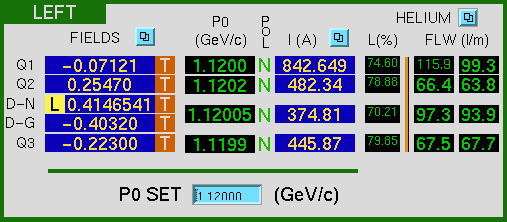
\includegraphics[angle=0,width=0.8\textwidth]{medm_halla_tools_1_cut1}
{\linespread{1.}
\caption[HRS: Magnets control]{A part of ``Hall A General Tools'' screen, 
        used for HRS (left) magnets control.}
\label{fig:hrs_mag_cntrl}}
\end{center}
\end{figure}

This box displays a brief summary of the status of the spectrometer
magnets and their cryogenic systems. The blue fields (with white
numbers) give readbacks of the magnetic fields and currents in each
magnet. The black fields also give readbacks, however in this case if
the text appears green those parameters are OK while if they are red
then that parameter is out of tolerance and may indicate a fault
condition. For example if the helium level goes below a certain point
the magnet will be automatically turned off.  In some cases it may be
desirable to monitor certain critical quantities on a strip chart
(e.g. magnet settings). A strip chart tool is available for this
purpose from the bottom of the ''EOS Menu'' button in the ''MyMenu'' window.

{\bf To set the spectrometers} for a given value of central momentum
(P0) type the desired P0 value into the light blue P0 SET box and hit
return. The magnets will be automatically 
set to the correct
values. All green numbers in the P0 column indicates that the desired
field or current settings have been reached. 

{\bf Caution:} Regarding the
dipoles, in general it's a bad idea to assume that at the first
instant that the P0 display turns green that the desired field has
been reached and you can start taking data. Stable field is in general
not achieved for from 15 to 30 minutes after reaching the nominal
desired field. This settling time depends on the magnet (the right dipole is
slower than the left dipole) and the magnitude of the field change (small
changes settle faster than big changes). Experimenters are advised to
observe both the field reading and current reading on the magnet in
question and verify that things are stable to their satisfaction
before proceeding.
 
\subsection{Powering Up Dipole Magnets:}

Use these instructions to recover from loss of a magnet due to a fault
(e.g. He level or lead flow fault). The order of actions matters. \\
(Contact Tech-On-Call if anything behaves funny or things don't
respond as expected. Sometimes after a trip an access to the Hall is
required to reset things).

\begin{list}{\arabic{enumi}.~}{\usecounter{enumi}\setlength{\itemsep}{-0.15cm}}
   \item Wait for Iout=0 (you can't and don't want to do anything while the magnet is in emergency fast dump mode.)
   \item While waiting, make a log entry re the fault. Give details such as time, coincident activities, and nature of the fault.
   \item Make sure the fault is cleared. (e.g. He level and flow rates returned to normal values and stable)
   \item In the HRS Right (Left) Dipole Systems' control panel:
   \begin{list}{}{\setlength{\itemsep}{-0.15cm}}
      \item[(a)] Press RESET (verify that all faults are cleared in the middle column)
      \item[(b)] Press ON (Display will indicate Power Supply ON and Magnet ENGAGED)
   \end{list}
\end{list}


Power supply and magnet are ready to go. From here you can return 
to "Autopilot Mode" (see Section \ref{sec:hrs-mag-set}).

\subsection{Starting Q1 Power Supply:}

 Do this when a fault causes the power supply to shut off.
 Wait for fault to clear (watch He levels). 
\begin{list}{\arabic{enumi}.~}{\usecounter{enumi}\setlength{\itemsep}{-0.15cm}}
   \item Push POWER OFF/RESET (check all faults cleared)
   \item Select desired polarity
   \item Push POWER ON
   \item Type in Setpoint (Amps) (light blue field) or re-enter P0 in Autopilot Mode.
\end{list}

\subsection{Starting Q2/3 Power Supply:}

 Do this when a fault causes the power supply to shut off.
 Wait for cause of fault to clear (watch He levels). 
 \begin{list}{\arabic{enumi}.~}{\usecounter{enumi}\setlength{\itemsep}{-0.15cm}}
   \item Push RESET 
   \item Select desired polarity
   \item Push ON
   \item Type in Current Set (light blue field) or re-enter P0 in Autopilot Mode.
\end{list}

} %infolev

\subsection{Rotation}
%
% Thanks to John LeRose for Rotation text. 07NOV2013
%
Moving an HRS
Since each HRS weighs in excess of 1,000 tons it is very important that all safety
precautions are carefully adhered to. The good news is they move very slowly (a few degrees/min
maximum), BUT 1,000 tons moving even very slowly is hard to stop. 

Hazards include:
\begin{itemize}
\item{Knocking items over.}
\item{The wheels crushing things (including fingers and toes) on the floor in the path of the 
spectrometer}
\item{Damaging the beamline or other equipment on the floor if one goes to too small 
or too large an angle, or if it just gets pushed around inadvertantly.}
\item{Tearing out of cables etc. physically attached to the superstructure}
\end{itemize}

Hazard mitigations:
\begin{itemize}
\item{Guards on either side of the wheels prevent items from getting under them.}
\item{Large pins in the floor to stop the spectrometer rotated beyond the needed angular range.}
\item{Blinking lights on the spectrometers indicating they are in motion or that motion
is possible (controls engaged etc.)}
\item{During a running experiment the run coordinator and work coordinator should know in advance 
of any moves.  Moves at any other time must be cleared with the Hall work coordinator 
before implementation.}
\item{Careful inspection of the intended path to make sure it is clear. This is part of
the pre-run checklist performed by the technical staff prior to closing the Hall and
a remote camera allows shift worker to inspect the area.}
%
%\item{Any motion that takes a spectrometer inside 14 degrees or outside x degrees
%(x being specified in the pre-run checklist and noted on the whiteboard during a run) 
%must be supervised by a trained Hall A technician.}
\end{itemize}

\infolevone{
Remote Procedure for a shift worker:
\begin{itemize}
\item{Make sure the move is part of the approved runplan (if in doubt, check with the 
run coordinator).}
\item{Check that the pre-run checklist has been completed and note and comply with any 
possible limitations to spectrometer motion (if there is a conflict inform the Run
Coordinator and do not initiate any move until the conflict is cleared).}
\item{Visually inspect the Hall using the closed circuit TV cameras to verify that there
are no obstructions.}
\item{If people are in the Hall wait until they leave (during a Controlled Access MCC keeps
track of people in the Hall). (Maybe we could soften this to "Inform EVERYONE in the Hall of
the move".)}
\item{Activate the spectrometer motion controls (see the Wiki and below) and 
move to the desired angle.}
\item{Deactivate the controls (brakes on, power off, etc.)}
\item{Update the spectrometer position information on the Hall A Controls screen}
\item{Make a halog entry indicating you've moved the spectrometer including from what angle 
to what new angle.}
\end{itemize}

Procedure for a non-run associated move in the Hall:
\begin{itemize}
\item{Inform the work coordinator of the planned move}
\item{Perform a careful visual inspection to verify that the path is clear}
\item{Check to make sure there are no temporary connections to the spectrometer (wires etc.)
that could be damaged during the move.}
\item{Inform everyone in the Hall of the move and check with them re 3.}
\item{Activate the spectrometer motion controls (see the Wiki and below) verify 
that the warning lights are on and move to the desired angle.}
\item{Deactivate the controls (brakes on, power off, etc.).}
\end{itemize}

The full proceedure for moving the spectrometer follows and can also be found on the Hall A wiki.

On hacsbc2, click the red "tool box" icon on the linux taskbar, as above. Choose 
bogies\_SetSpec so that you can determine the angle and vernier setting for the spectrometer.
Enter the spectrometer (L or R), and the angle, and you will get two options for the floor 
mark and the vernier. Generally choose the vernier closer to zero. Center the cameras on the 
desire vernier using the Move+/Move- buttons on the Hall A General Tools screen. The TV monitors 
for these cameras are on the middle shelf, in rack CH01A05.

Choose bogies\_Left (or bogies\_Right) in the tool box to bring up the bogies control screen. 
Click PSM enable and wait a few seconds for PSM OK to read YES. 
Click DM enable and wait a few seconds for DM OK to read YES.
Make sure the velocity is set to 0 and the direction is CW or CCW as desired. Click on Brake Release 
and wait for Brakes OK to read YES.

Click on ClampRelease, set the velocity to 700. Once you see the spectrometer start to move in the 
floor angle camera - you cannot see the spectrometer move in the Hall overview camera, as it only 
moves a few degrees per minute at maximum speed. For the left arm, to move to a larger angle, the 
direction should be CCW, while for the right arm CW moves the spectrometer to larger angle. The 
direction of the spectrometer is reversed by using a negative rpm. Watch the spectrometer motion 
on the cameras. When you are getting close to the desired angle, slow down to about 300 rpm. 
To stop, click on the Clamp Release button and the Brake button. Disable DM and PSM, and disconnect 
to close the GUI. Read off the floor angle mark and vernier, and input the values into the appropriate 
fields in the Alignment section of the Hall A General Tools GUI. 
}









\newpage
\section[Field Monitoring]{Field Monitoring
\footnote{
  $CVS~revision~ $Id: nmr-1999.tex,v 1.4 2003/12/17 03:59:48 gen Exp $ $ 
}
\footnote{Authors: J.LeRose \email{lerose@jlab.org}}
}

The field-monitoring controls are available using the main 
HRS screen%
\infolevtwo{ (see Figure~\ref{fig:hrs_mag_cntrl})%
}. % infolev
The dipoles' field is measured using NMR Teslameters and
field probes.

\infolevone{ 
 
\subsection{ Dipole Field Monitoring Electron Arm}

\noindent {\bf Basic Setup}

Each spectrometer dipole magnet is equipped with a Metrolab PT 4025 
NMR Teslameter, several field probes, and multiplexers (to allow switching 
between the probes).  Details of the operation and theory of operation 
for the Teslameter can be found in its user manual, 
a copy of which is available in the the counting house.
The basic layout is shown in Figure~\ref{fig:nmrbasic}


\begin{figure}
\begin{center}
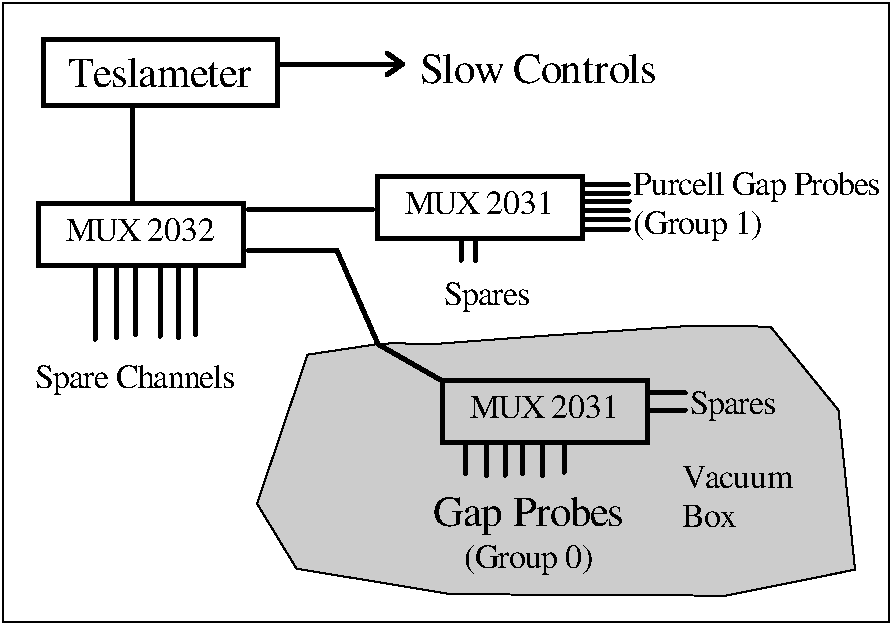
\includegraphics[angle=0,width=15cm,clip]{lerose_fig1}
{\linespread{1.}
\caption[Spectrometers: NMR System Layout]{Basic layout of NMR system}
\label{fig:nmrbasic}}
\end{center}
\end{figure}


 The "Gap Probes" (Group 0 in the controls) are located in two groups 
of three; one group on the low field side of the gap and the other on the high 
field side of the gap.  The groups of three are made up of one each of 
the manufacturer's type 3, 4 \& 5 probes, designed to cover different 
field ranges (see Table \ref{nmr_range}).  The six ``Purcell Gap Probes'' (Group 1 in 
the controls) are located in the Purcell gap of the magnet 
and consists of two each of the above types. {\em Note: Since
the fall of 1998 the multiplexer-multiplexer in both arms,
MUX 2032, has been removed and hence the ``Purcell Gap Probes'' are currently
unavailable. There are no plans to re-install this multiplexer.}

 The "Gap Probes" are equipped with coils which provide a field 
gradient that cancels out the field gradient of the magnet in the vicinity of 
the probe.  These gradient compensating coils are part of a simple circuit 
that is completely independent of the Teslameter.  The basic circuit for 
the compensating coils is shown in Figure~\ref{fig:nmrcir}


\begin{figure}
\begin{center}
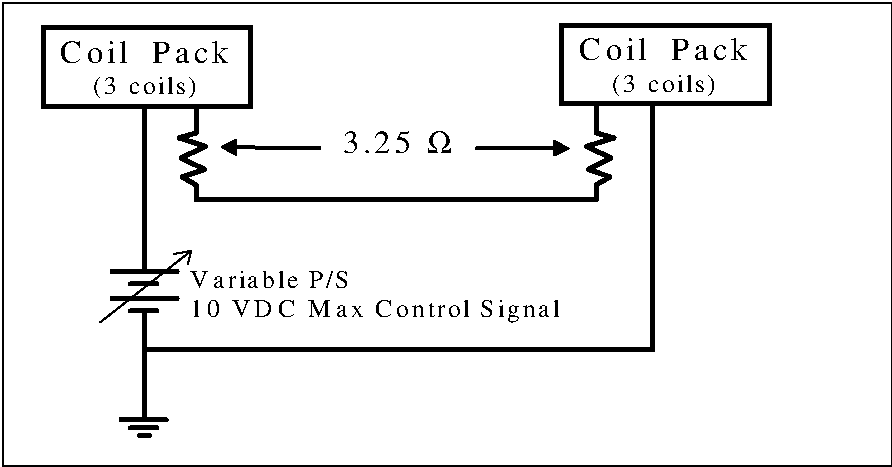
\includegraphics[angle=0,width=10cm,clip]{lerose_fig2}
{\linespread{1.}
\caption[Spectrometers: NMR Gradient Compensation]{Gradient Compensating Circuit.}
\label{fig:nmrcir}}
\end{center}
\end{figure}


%\snfig{figs/lerose_figcce.eps}{Control Voltage calibration for
%Electron Dipole }{nmrcomp4}{5in}

\begin{figure}
\begin{center}
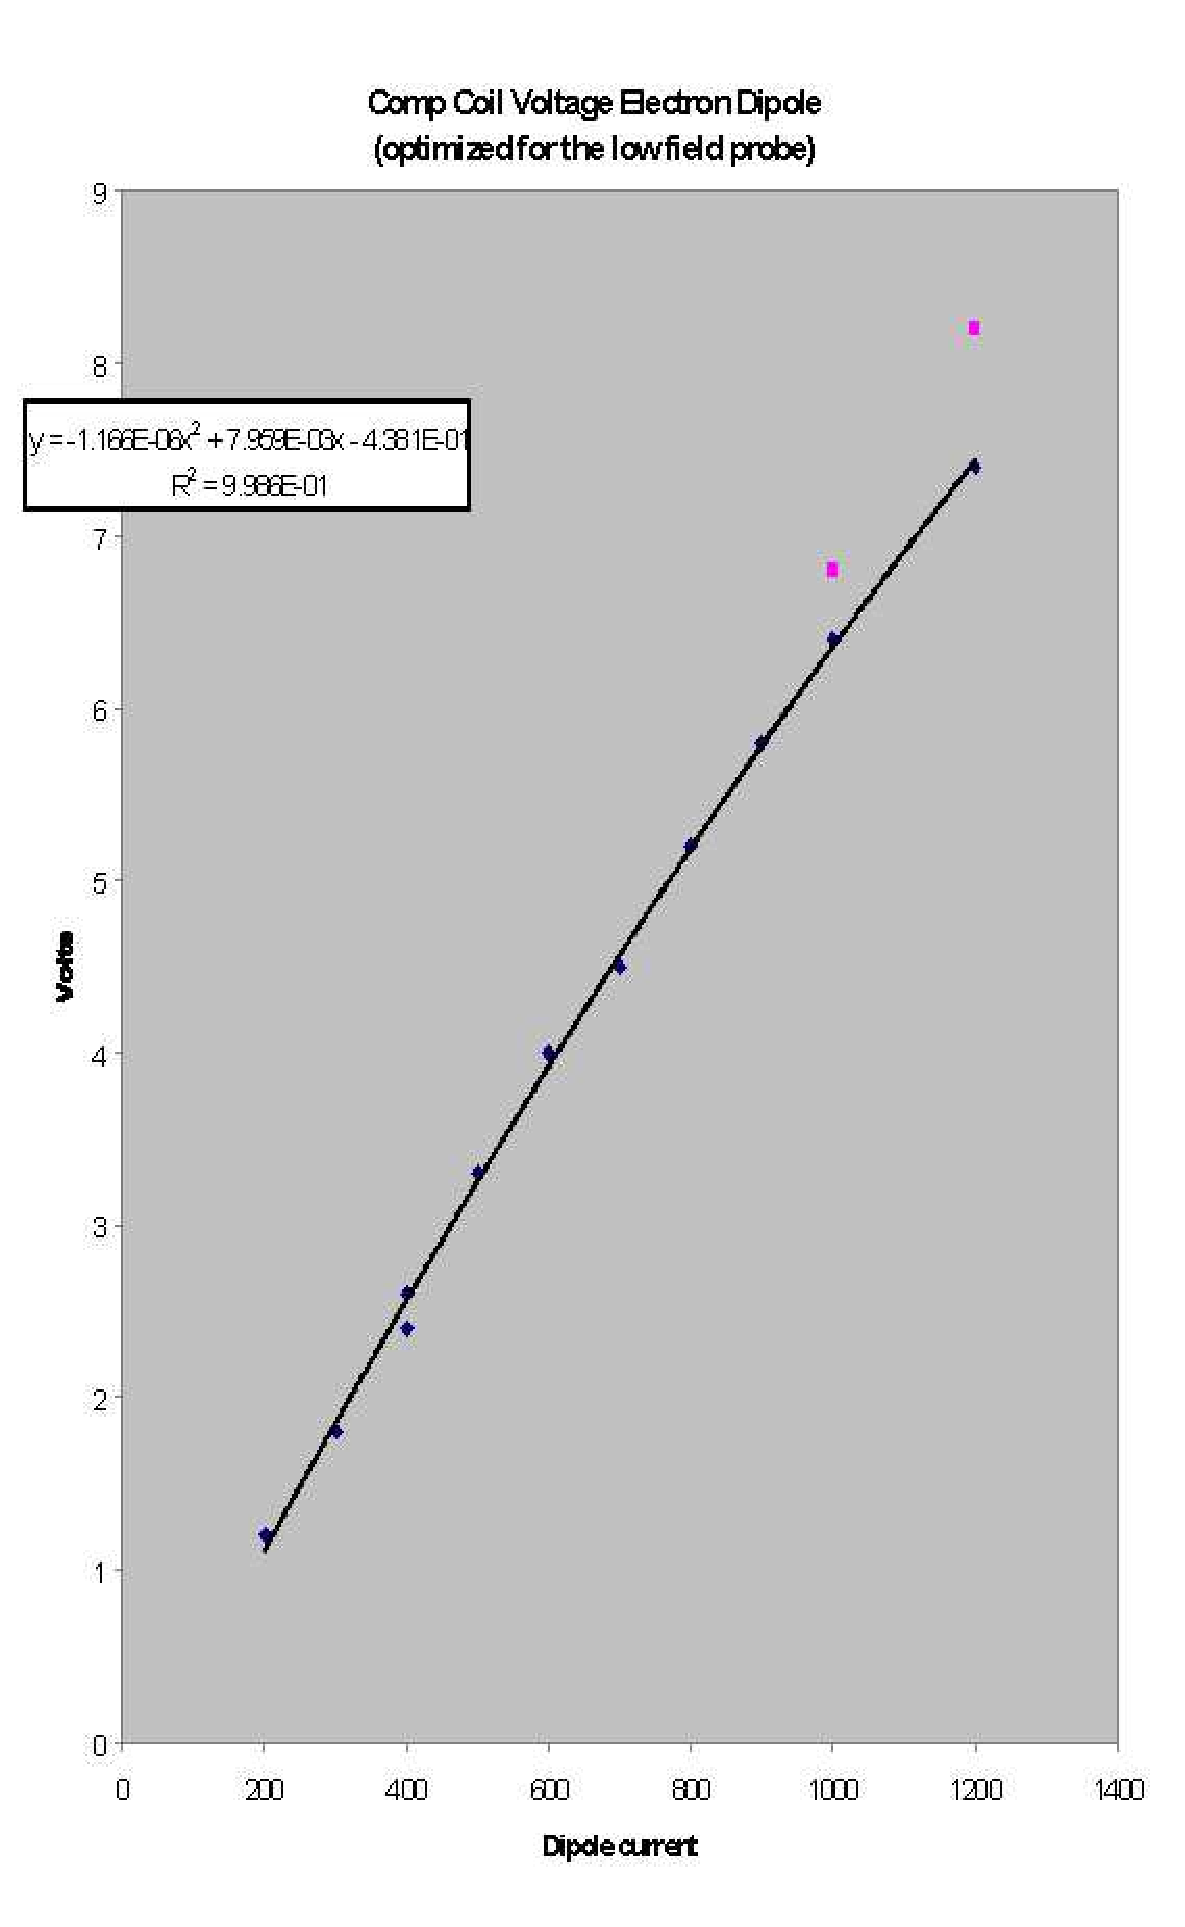
\includegraphics[angle=0,height=20cm,clip]{lerose_figcce}
{\linespread{1.}
\caption[Spectrometers: Control Voltage Calibration for Left Dipole]{Control Voltage calibration for the Left Dipole.}
\label{fig:nmrcomp4}}
\end{center}
\end{figure}

%\snfig{figs/lerose_figcch.eps}{Control Voltage calibration for
%Hadron Dipole }{nmrcomp5}{5in}
\begin{figure}
\begin{center}
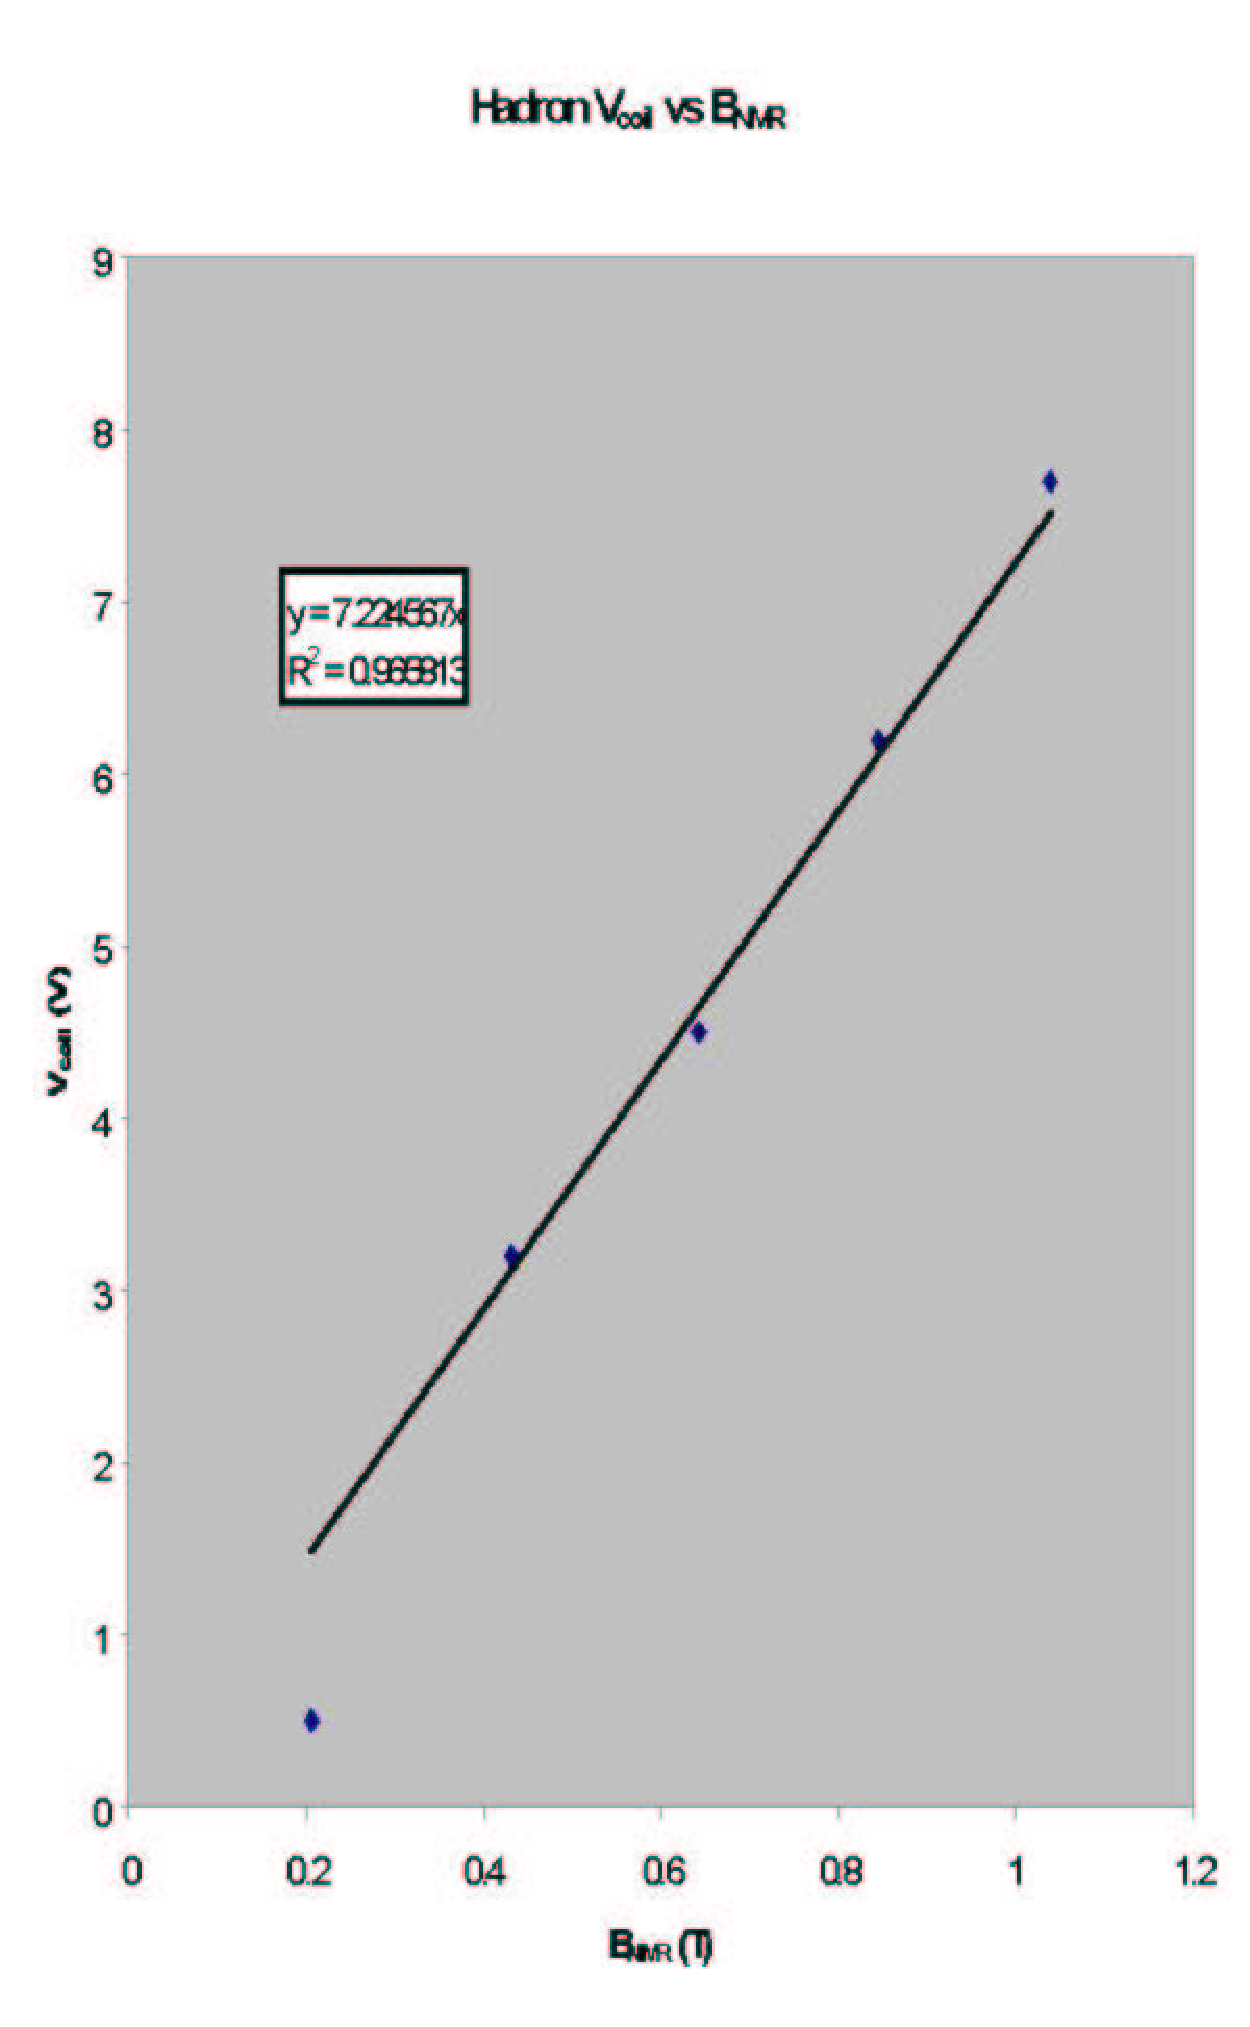
\includegraphics[angle=0,height=20cm,clip]{lerose_figcch}
{\linespread{1.}
\caption[Spectrometers: Control Voltage Calibration for Right Dipole] {Control Voltage calibration for the Right Dipole.}
\label{fig:nmrcomp5}}
\end{center}
\end{figure}

%\snfig{./figs/lerose_fig7.eps}{DAC Calibration for manual operation of NMR probes}{nmr_dac}{9in}
\begin{figure}
\begin{center}
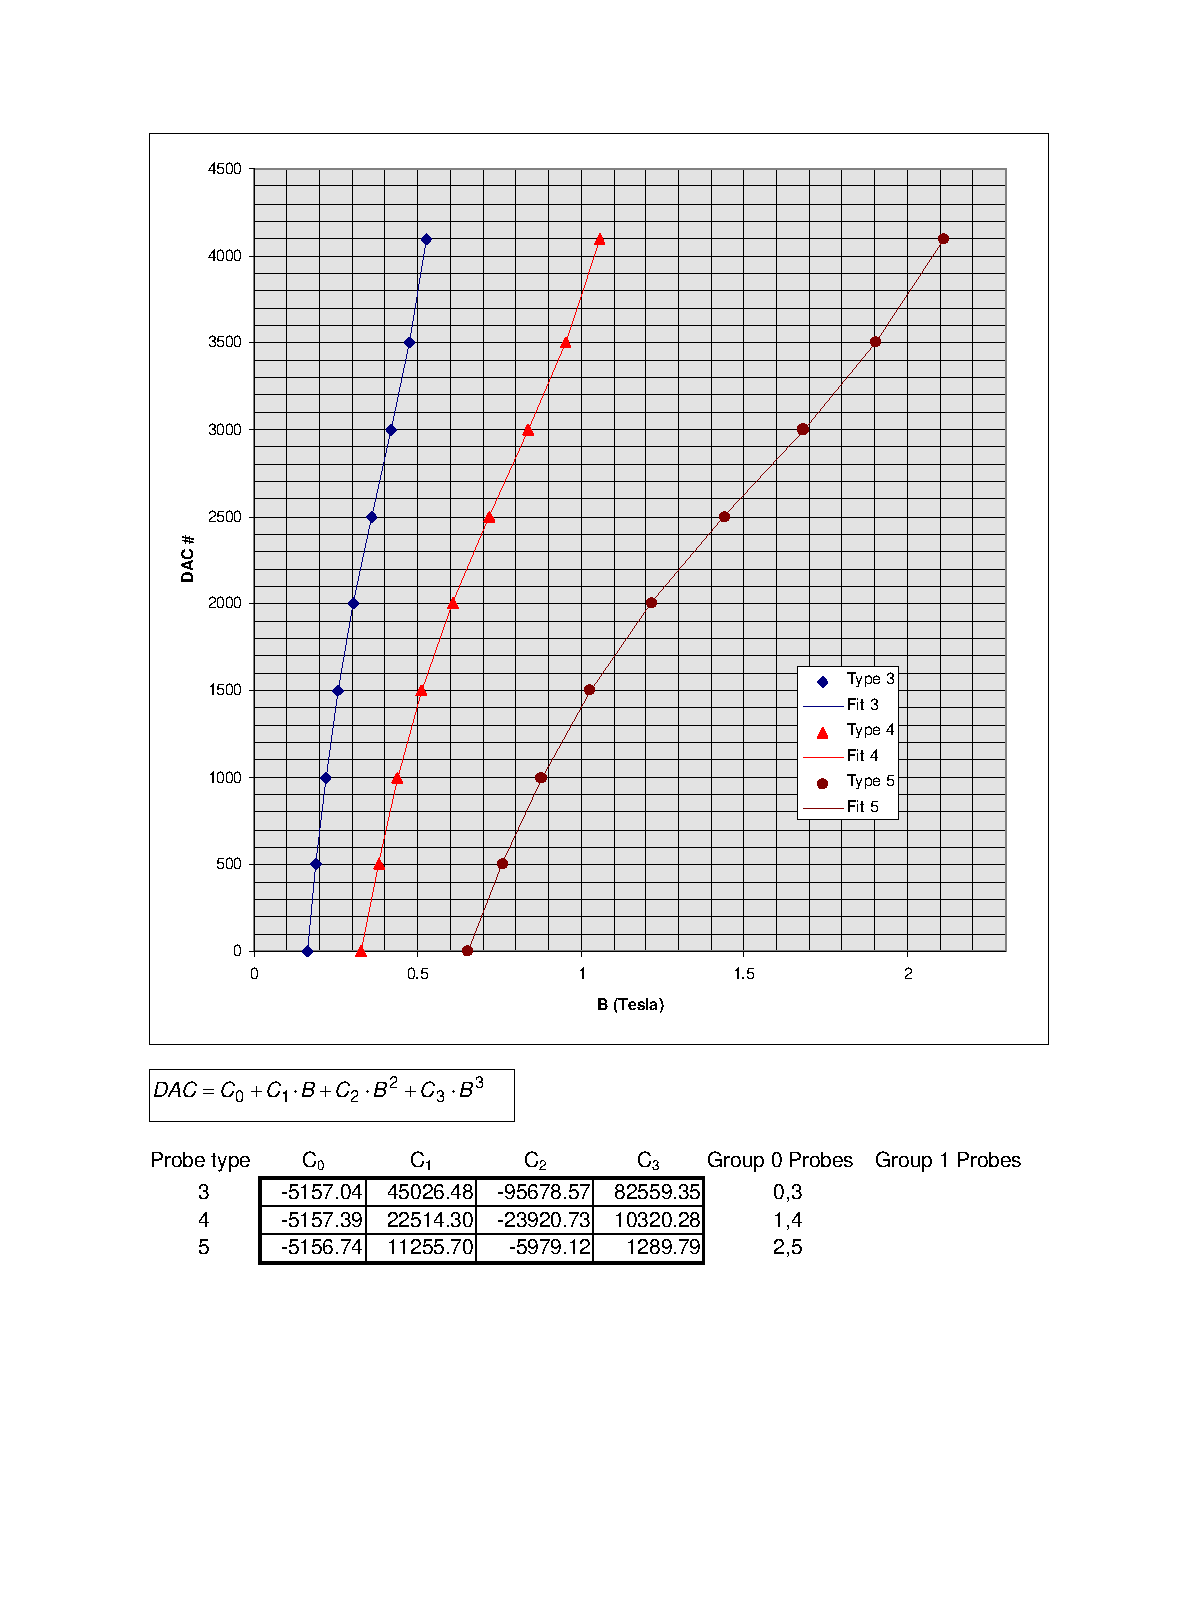
\includegraphics[angle=0,height=20cm,clip]{lerose_fig7}
{\linespread{1.}
\caption[Spectrometers: NMR Probe DAC Calibration]{DAC Calibration for manual operation of NMR probes.}
\label{fig:nmr_dac}}
\end{center}
\end{figure}

The following graphs (see Figures~\ref{fig:nmrcomp4} 
and ~\ref{fig:nmrcomp5}),can be used to determine optimum values for the 
compensating coil control voltage.  It should be noted that the setting 
of the compensating coil current is not very critical in most cases.  In 
general if you're within 10\% of the correct value everything should 
work fine.



\begin{table}
\begin{center}
\begin{tabular}{|cc|} \hline
Probe Type & Field Range (T) \\ \hline 
3 & 0.17 - 0.52 \\
4 & 0.35 - 1.05 \\
5 & 0.70 - 2.10 \\ \hline
\end{tabular}
\caption[Spectrometers: Dipole NMR Probe Field Ranges]{Dipole NMR probe field ranges}
\label{nmr_range}
\end{center}
\end{table}

} %infolev

\infolevtwo{
\subsection{NMR Operating Procedure}

When running in Autopilot mode (see: Simple Spectrometer Field Setting) the 
compensating coil voltage is set automatically and the probe appropriate for 
the field desired is selected. The gaussmeter is placed in SEARCH Mode and the 
dipole power supply software regulator is turned on. In this case the dipole current is 
adjusted to achieve the desired field. The user should just stand 
back and let it work. What follows are instructions for using
the NMR gaussmeter in situations where Autopilot doesn't work or
some special supplemental measurements are required. 

 In principle it is possible to make the field measurements using the 
SEARCH mode in the Teslameter.  In this mode you select a probe and the 
meter explores the whole field range of the probe until it finds and 
"locks" on the resonant signal indicating that it has a field 
measurement.  A ``lock" is indicated on the controls display by an ``L'' to 
the left of the field values.  This has the advantage of simplicity but in practice can 
be time consuming and doesn't always work.  The problem being, in 
situations where there is a lot of noise mixed in with the signal, the 
circuitry has problems distinguishing the signal from the noise and gets 
lost before it ever finds a lock.  The problem is exacerbated when the 
field being measured is at the high end of the probe's range.  In this 
case the search starts at the low end and keeps getting hung up on the 
noise and never gets to the field range of interest.  The solution to 
this problem is to tell the device approximately what field it's looking 
for and use the AUTO mode to find the lock.  In the procedure below that 
is what we will be doing.

In any case, for ``gap probes" (group 0) you must energize and adjust 
the gradient compensating coils for the field ranges to be measured before 
trying to make a measurement.

For studies involving 
10\% changes in the field settings the compensating coil current can be 
set once and left alone.


\noindent\underline{\bf Recommended Procedure:}(turn the {\bf SOFTWARE REGULATOR OFF} for all 
non-autopilot field measurements)\\
For group 0 probes set compensating coils appropriately (see figures).\\
Put the meter in MANUAL mode with SEARCH OFF \\
Select a probe \underline{\bf and} polarity (\underline{\bf Group 0:  
Probes 0, 1, 2 negative; Probes 3, 4, 5 positive}) \\
Type in the appropriate DAC number for the field range being measured (see below) \\
Select AUTO and wait for a lock (indicating a valid field reading) \\
Verify that you have a good lock by checking the oscilloscope for a 
clear resonant signal. \\
If you have problems see the table listing problems and possible 
solutions.

\noindent\underline{\bf Selecting DAC Number}

In selecting the DAC number to use for the field of interest use 
either the graph in Figure~\ref{fig:nmr_dac} or the polynomial at the bottom of the same figure.

\pagebreak
\noindent{\bf Problems and Solutions}\\
\begin{table}[htb]
\begin{tabular}{|p{0.4\textwidth}|p{0.55\textwidth}|}\hline
Symptom & Diagnosis and Cure \\ \hline\hline
Weird numbers on displays, controls for all magnets fouled up 
& Need to reboot.  See instructions below. \\ \hline
NMR Teslameter does not respond to commands and display shows all zeros. 
& Meter's communications are somehow hung up. Push {\bf RESET}. \\ \hline
%Will not lock & Very high noise level makes resonance hard to find. \\
%Still 
Will not lock 
& Very high noise level makes resonance hard to find. Search for the resonance manually by 
  adjusting the DAC in manual mode until you see the resonant signal.  (It helps if you know 
  what field you expect so you'll know where to look). \\ \hline
You find resonance manually but still can't get a lock 
& Check probe polarity. Try decreasing and increasing DAC number by 1. Optimize signal 
  by adjusting compensating coils. \\ \hline
Can't find resonance manually 
& Try a different probe.  Use readings from other probes to tell you where to look for 
 the resonance with the probe that's giving you trouble.  Make sure
 compensating coils are energized properly.  Make sure magnet is on. \\ \hline\hline
\end{tabular}
\caption[NMR: Problems and solutions]{NMR: Problems and solutions}
\label{tab:nmr-problems-solutions}
\end{table}

\begin{table}[ht]
\begin{center}
\begin{tabular}{|p{0.3\textwidth}|p{0.3\textwidth}|p{0.3\textwidth}|}\hline
Problems & Explanation & Action \\ \hline
NMR not locked but current is changing in the right direction 
& Normal operation for large field changes  
& Wait. (see above) \\ \hline
NMR locked but current going in the wrong direction.
& Normal operation. 
& Wait. \\ \hline
NMR locked but field not correct and current not changing 
& Field regulation is disabled or software is confused.
& Check that field regulation is enabled. Enter desired field value or one
  very near the desired value again. \\ \hline
NMR field display freezes. (Usually but not always shows  -\#.0000000)
& NMR Gaussmeter is not communicating with software.
& Push {\bf RESET}. \\ \hline
\end{tabular}
\end{center}
\caption[NMR troubleshhoting]{NMR troubleshooting
}
\label{tab:hrs_nmr_2}
\end{table}

} %infolev

\begin{safetyen}{10}{15}
\subsection{Authorized Personnel}
\end{safetyen}

The individuals shown in Table \ref{tab:nmr:personnel} are responsible for NMR operation problems.

\begin{namestab}{tab:nmr:personnel}{NMR: authorized personnel}{%
      NMR: authorized personnel.}
  \JavierGomez{\em Contact}
  \JohnLeRose{}
\end{namestab}



\newpage
\section[Collimators and Sieve Slits]{Collimators and Sieve Slits
\footnote{
  $CVS~revision~ $Id: slit.tex,v 1.5 2003/12/13 06:23:38 gen Exp $ $ 
}
\footnote{Authors: J.LeRose \email{lerose@jlab.org}}
}

Both spectrometers have front-end devices for calibrating the optical
properties of the spectrometers. These are known as the collimator boxes.
These boxes are positioned between the scattering chamber and the 
first quadrupoles (Q1). Each box is carefully aligned and rigidly attached
to the  entrance flange of the Q1 of the respective spectrometer.  The boxes are
part of the vacuum system of the spectrometer.
In the septum configuration sieve slits and collimators are installed and removed manually.

Inside each box a ladder is mounted which is guided by a linear bearing
and moved up and down by a ball screw. On this ladder 3 positions are 
available to insert collimators. Below this ladder
a special valve is mounted that can isolate the vacuum in the spectrometer
from the target system. This valve should be activated when it is moved
in front of the holes connecting the box with spectrometer and target chamber.
\infolevone{
A schematic view of the collimator box is shown in Fig.~\ref{fig:coll}.

\begin{figure}
\begin{center}
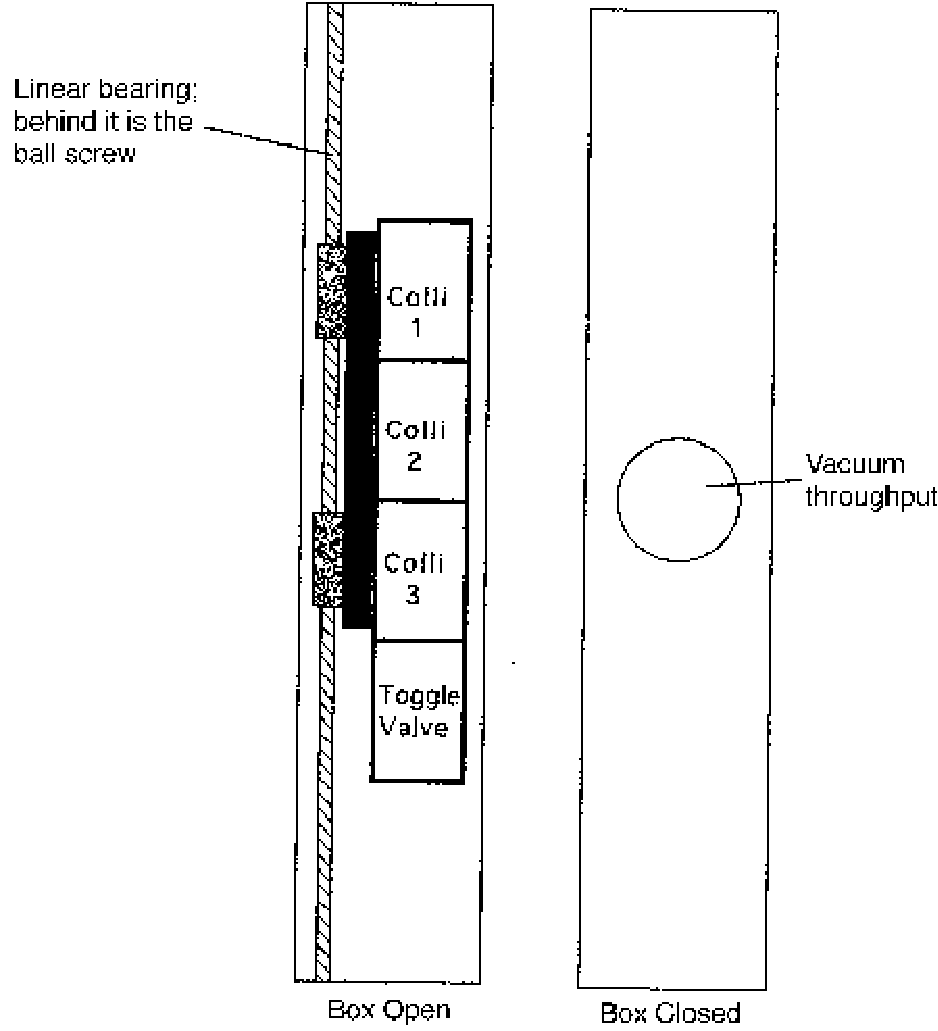
\includegraphics[angle=0,width=13cm,clip]{collimator_clip}
{\linespread{1.}
\caption[Spectrometers: Collimator Box Schematic]{Schematic layout of the collimator box.}
\label{fig:coll}}
\end{center}
\end{figure}
} %infolev

Vacuum requirement is $10^{-6}$ Torr. The material for the box is 
aluminum. It is possible to open one side of the box so that
collimators can be exchanged. The
reproducibility of collimator positions after moving
the ladder and/or after replacing a collimator is
better than 0.1 mm in horizontal and vertical direction.
The dimensions of the box are
roughly height=175 cm , width=35 cm and depth=15 cm.
The tolerance in the dimension
of the 7 msr collimator hole is $\pm0.5$ mm in each direction. 
The tolerance in the position
of each of the sieve-slit holes is $\pm0.1$ mm in each direction.

\infolevone{
\begin{figure}
\begin{center}
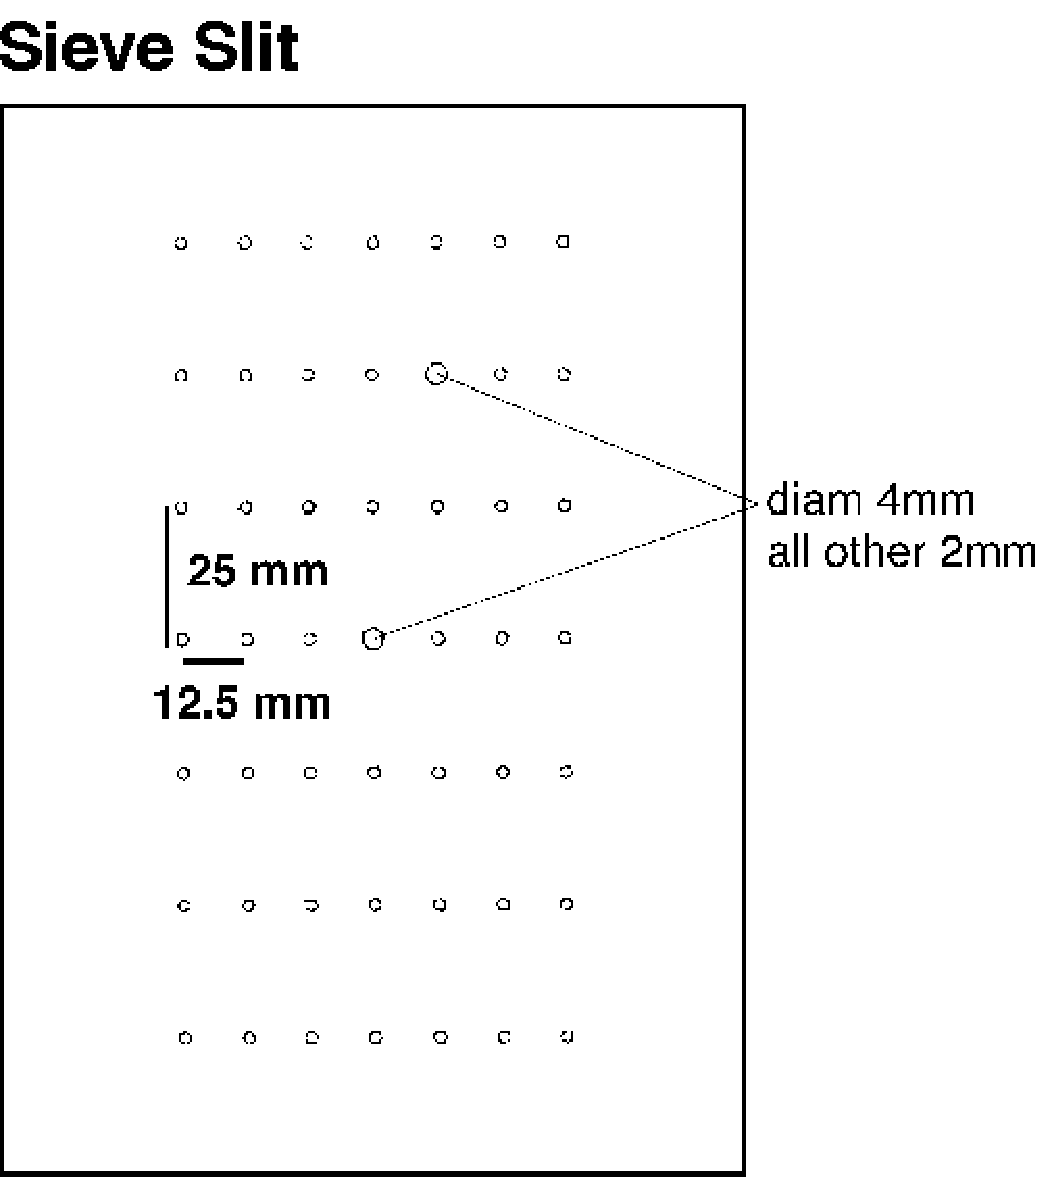
\includegraphics[angle=0,width=13cm,clip]{sieveslit}
{\linespread{1.}
\caption[Spectrometers: Sieve Slit]{Sieve slit collimator for optics calibration.}
\label{fig:sieve}}
\end{center}
\end{figure}
} %infolev
A typical sieve slit collimator 
\infolevone{(shown in Fig.~\ref{fig:sieve})
} %infolev 
consists of a plate of roughly 14 cm x 20 cm containing 49 holes
positioned in a regular 7x7 pattern. This slit is made out of 5
mm thick tungsten.
The holes have a diameter of 2 mm except for the central one and one positioned
off-diagonal which have a diameter of 4 mm. The horizontal distance between the
holes is 12.5 mm while the vertical distance is 25.0 mm.
%
%To get the latest information on the dimensions and locations of the collimators see 
%the Hall A homepage on the web%
%\htmladdnormallinkfoot{}{\url{
%http://hallaweb.jlab.org/
%}}.

To get the latest information on the dimensions and locations of the collimators see 
the Hall A homepage on the web%
\htmladdnormallinkfoot{}{\url{
http://hallaweb.jlab.org/
}}.

\begin{safetyen}{10}{15}
\subsection{Safety Assessment}

The collimator boxes form part of the vacuum system for each spectrometer. All hazards
identified in section spectrometer vacuum section applies to the collimator box as well.

In addition, safe access to the top of
the collimator boxes is needed  during manual operation of the box as outlined below.
Due to the proximity of the collimator boxes to the scattering chamber, and Q1 quadrupoles,
all necessary safety precautions with regards to vacuum windows, electrical power cables, 
cryogenic transfer lines, and high magnetic field should be taken. The same precautions also apply 
to the collimators and sieves in the septum configuration. In that case the sieve and collomators
can be considered part of the beamline. A survey and
appropriate RADCON designated proceedures must be followed when dealing with septum sieves 
and collimators.
\end{safetyen}

\infolevtwo{
\subsection{Operating Procedure}
Slit position is changed remotely from the standard Hall A control screen.
In the case of a spectrometer configuration involving the septum magnets collimators and sieves are
changed manually in the Hall.
} %infolev

\subsection{Authorized  Personnel} 

\begin{itemize} 
\item[~]E. Folts - x7857 (mechanical and vacuum systems).
\item[~]J. Gomez - x7498 (computer controls and electrical systems).
\end{itemize} 

% ===========  CVS info
% $Header: /group/halla/analysis/cvs/tex/osp/src/hrs/slit.tex,v 1.5 2003/12/13 06:23:38 gen Exp $
% $Id: slit.tex,v 1.5 2003/12/13 06:23:38 gen Exp $
% $Author: gen $
% $Date: 2003/12/13 06:23:38 $
% $Name:  $
% $Locker:  $
% $Log: slit.tex,v $
% Revision 1.5  2003/12/13 06:23:38  gen
% Septum added. Name tables. Polishing
%
% Revision 1.4  2003/12/05 06:49:07  gen
% infolevels added, polishing
%
% Revision 1.3  2003/06/06 16:13:37  gen
% Revision printout changed
%
% Revision 1.2  2003/06/05 23:30:00  gen
% Revision ID is printed in TeX
%
% Revision 1.1.1.1  2003/06/05 17:28:31  gen
% Imported from /home/gen/tex/OSP
%
%  Revision parameters to appear on the output

\newpage
\infolevtwo{
\section[Spectrometer Alignment]{Spectrometer Alignment
\footnote{
  $CVS~revision~ $Id: AlignmentOps.tex,v 1.8 2003/12/17 03:59:48 gen Exp $ $ 
}
\footnote{Authors: J.Gomez \email{gomez@jlab.org}}
}

At present, the systems implemented to determine the alignment of each spectrometer
(roll, vertical angle/pointing and horizontal angle/pointing) without the help of the
Accelerator Division Survey group are limited to roll, vertical angle and horizontal angle.
All alignment information is displayed in the ``ALIGNMENT'' mosaic of the ``Hall A
General Tools'' EDM screen%
\infolevtwo{ (see Fig.~\ref{fig:medm-hlamain-tools})}
(``EOS Menu'' $-->$ ``EDM (HLA Main)'' $-->$ ``Hall A Main Menu'' $-->$ ``Tools'').

A bi-axial inclinometer is used to determine the roll and vertical angle (also known as pitch)
of each spectrometer. These inclinometers are attached to the back of the dipoles at the power
supply platform level. The raw inclinometer measurements, in Volts,
are displayed as ``Tilt X'' and ``Tilt Y''. The inclinometer temperature is also given
(`` Tilt T''), in degree Celsius. From these values, the ``ROLL'' and ``PITCH'' values are
calculated.
Agreement between the inclinometer readings and survey measurements
are better than $\pm$ 0.1 mrad over all presently available history.

The horizontal spectrometer angle is determined from floor marks set in
place by the survey group. Floor marks have been placed every 0.5 $^\circ$ covering the useful range of
both spectrometers.
There are two concentric rings of floor marks in the hall. We will concentrate in the
inner ring which covers the angular range of both spectrometers. The outer ring is
similar.
The inner-ring floor marks are located at a distance of $\sim$10 $m$ from the target center.
A ruler attached to each spectrometer dipole runs over the floor marks and it acts as a vernier to interpolate
between marks. The location of a given floor mark on the ruler can be viewed from the Hall A Counting
House through a TV camera (labeled ``Front Camera'') .
The camera is able to move along the length of the ruler so that any
parallax effect can be eliminated. The camera motion is controlled from the ``Tools'' screen
through two push buttons (``FRONT CAMERA'' - ``MOVE +'' and ``MOVE --'').
Two fields in the ``ALIGNMENT'' mosaic
(``Flr Mrk'' and ``Vernier'') allow to input
the values read from the TV monitor. The effective spectrometer angle is then calculated and displayed
as ``Angle''. The application ``HRS Floor Marks'' calculates the floor mark and vernier value
to which the spectrometer should be set
to obtain a given angle. Spectrometer horizontal angle surveys and floor mark determinations
agree to $\pm$ 0.2 mrad.

\newpage
\begin{safetyen}{10}{15}
\subsection{Authorized  Personnel} 
\end{safetyen}
The authorized personnel is shown in table \ref{tab:align:personnel}.
\begin{namestab}{tab:align:personnel}{HRS alignment: authorized personnel}{%
      HRS alignment: authorized personnel.}
  \JessieButler{\em Contact}
\end{namestab}

} %infolev


% ===========  CVS info
% $Header: /group/halla/analysis/cvs/tex/osp/src/hrs/all.tex,v 1.3 2003/06/06 15:44:08 gen Exp $
% $Id: all.tex,v 1.3 2003/06/06 15:44:08 gen Exp $
% $Author: gen $
% $Date: 2003/06/06 15:44:08 $
% $Name:  $
% $Locker:  $
% $Log: all.tex,v $
% Revision 1.3  2003/06/06 15:44:08  gen
% Revision printout changed
%
% Revision 1.2  2003/06/05 23:30:00  gen
% Revision ID is printed in TeX
%
% Revision 1.1.1.1  2003/06/05 17:28:31  gen
% Imported from /home/gen/tex/OSP
%
%  Revision parameters to appear on the output

\chapter{High Resolution Spectrometers (HRS)}
\graphicspath{{hrs/figs/}}
\renewcommand{\dirfig}[0]{hrs/figs}
\renewcommand{\dircur}[0]{hrs}

\infolevone{
\chapter[High Resolution Spectrometers (HRS)]{High Resolution Spectrometers (HRS)
}
\footnote{Authors: J.LeRose \email{lerose@jlab.org}}
}
\label{chap:hrs}

\infolevone{
\section{Overview}
   
The Hall A spectrometers and associated instrumentation are designed to 
perform high resolution and high accuracy experiments.  The goal is to 
achieve a missing mass resolution of $\sim$ 200-500 keV to clearly 
identify the nuclear final state.  An absolute accuracy of $\sim$ 1\% is 
also required by the physics program planned in the Hall, which implies 
$\sim$ 10$^{-4}$ accuracy in the determination of particle momenta and 
$\sim$ 0.1 mr in the knowledge of the scattering angle.

The instruments needed are a high resolution electron spectrometer 
(HRES) and a high resolution hadron spectrometer (HRHS), both with a 
large angular and momentum acceptance.

\begin{figure}[tbp]
\begin{center}
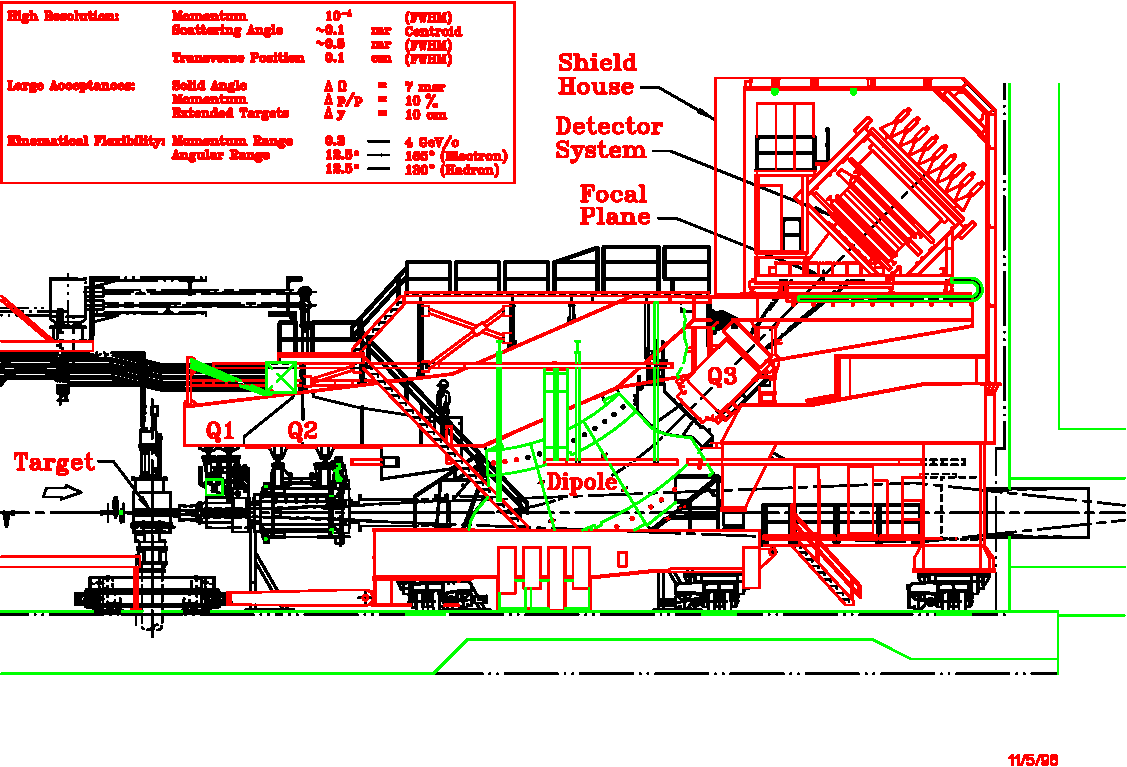
\includegraphics[angle=0,width=0.9\textwidth,clip]{figure0101_r}
\caption[Spectrometers: Elevation View of Hall~A HRS]{A side view of the Hall~A
HRS spectrometer.}  
\label{fig:hrs_ev}
\end{center}
\end{figure}
 
\begin{figure}[tbp]
\begin{center}
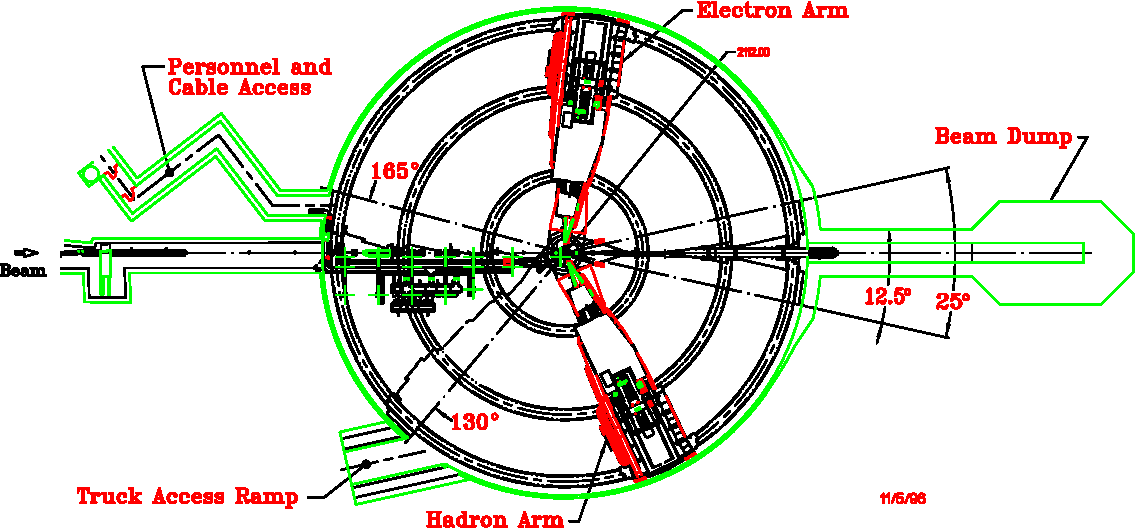
\includegraphics[angle=0,width=0.9\textwidth,clip]{figure0102_r}
\caption[Spectrometers: Plan View of Hall~A]{A bird's eye view of the Hall~A
end-station at TJNAF.}  
\label{fig:hrs_pv}
\end{center}
\end{figure}


A layout of the 4 GeV/c High Resolution Electron Spectrometer is shown 
on Figures~\ref{fig:hrs_pv} and \ref{fig:hrs_ev}.
Its main design characteristics are 
given in the attached table.  The spectrometer has a vertical bending 
plane and 45$^{\circ}$ bending angle.  The QQDQ design includes four 
independent superconducting magnets, three current-dominated 
cos2$\theta $ quadrupoles and one iron-dominated dipole with 
superconducting racetrack coils.  The second and third quadrupoles of 
each spectrometer have sufficiently similar field requirements that they 
are of identical design and construction.  The overall optical length, 
from target to focal plane, is 23.4 m.  Optically, the HRHS 
is essentially identical to HRES. In fact the two spectrometers can be used 
interchangeably to detect either positively or negatively charged particles 
as needed by any particular experiment. They are now commonly refered to 
as ``The Left Arm'' and ``The Right Arms'' rather than ``Hadron'' and ``Electron'' 

The support structure includes all system elements which bear the weight 
of the various spectrometer components and preserve their spatial 
relationship as required for 45$^{\circ}$ vertical bending optics.

The alignment and positioning system includes all the elements which 
measure and adjust the spatial relationship.  The support structure 
consists of the fabricated steel components which support the magnets, 
detector, shield house and associated equipment.  It is composed of the 
box beam, which supports the outer elements in fixed relative position 
atop the dipole; the dipole support bracket, upon which the dipole rests on 
the jacks; the cradle, upon which the dipole rests through the vertical 
positioning system, VPS; and a portion of the shield house load through 
the inboard legs of the gantry; the gantry, which supports the shield 
house and the magnet power supplies; and the bogies, which support the 
cradle-gantry assembly and roll on the floor plates and provide the 
driving power to move the two spectrometer arms.

The detector package (described in detail in Chapter \ref{chap:hrs-det})
is supported on the box beam and is surrounded by 
the shield house.  It must perform two functions, tracking and particle 
identification, PID.  The most important capability of focusing 
spectrometers is measuring precisely the momenta and entrance 
orientations of the tracks.  Momentum resolution of 10$^{-4}$ is 
obtainable, consistent with the resolution of the incident beam.

The actual configuration of the detector package varies from experiment to
experiment. The description given here is only an example of what is possible.
}

\infolevone{
A particle traversing the detector stack 
(Figure~\ref{fig:hrs_electron_det}) encounters two sets of horizontally
mounted, vertical drift wire chambers (x,y) with two planes of 368
wires in each chamber. The track resolution is $\sim$ 100 $\mu$m.  
From the chamber information both 
positions and angles in the dispersive and transverse directions can be 
determined.  The information from these chambers is the principal input 
of the tracking algorithms.

The chambers are followed by a scintillator hodoscope plane designated S1. 
This plastic scintillator array provides the timing reference for 
the drift chambers, and is also used in trigger formation and in combination 
with a second hodoscope pair it can provide time of flight particle 
identification.  These scintillators can also be used to perform crude 
tracking.

The next element encountered by a particle is a gas threshold \Cherenkov{} 
detector.  This is used for particle identification.  This gas threshold \Cherenkov{} detector can be swapped 
against an Aerogel detector, with a similar function.

The second hodoscope plane, S2, is located directly behind the 
gas \Cherenkov{}.  Its function is essentially the same as that of S1.  
In the hadron spectrometer an option exists to have this hodoscope 
pair be preceded by a third chamber, to improve tracking.
 Each of the two spectrometers 
have gas and Aerogel \Cherenkov{} detectors which can be used
 when they are in electron detection mode.

The final elements in the detector stack on HRSE are 
the pre-shower and the total-absorber lead glass shower 
calorimeter.  This is used for energy determination and PID.

\begin{figure}[tbp]
\begin{center}
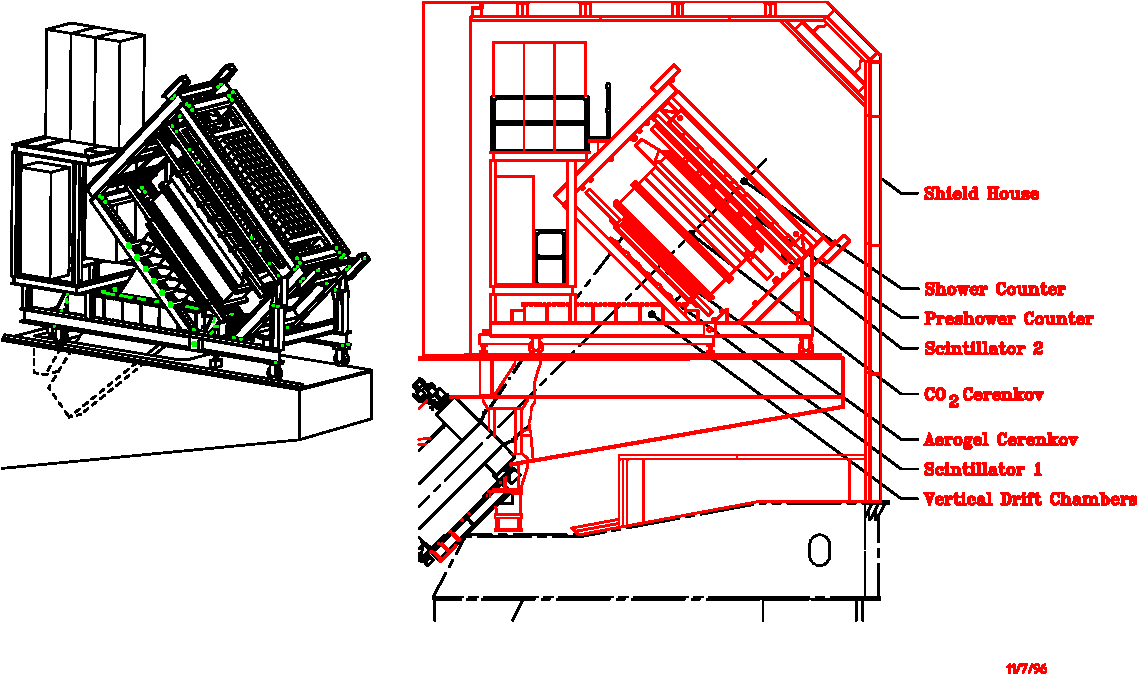
\includegraphics[angle=0,width=\textwidth,clip]{figure0103_r}
{\linespread{1.}
\caption[Spectrometers: Electron Arm Detectors]{The electron spectrometer detector stack.}
\label{fig:hrs_electron_det}}
\end{center}
\end{figure}

\begin{figure}[tbp]
\begin{center}
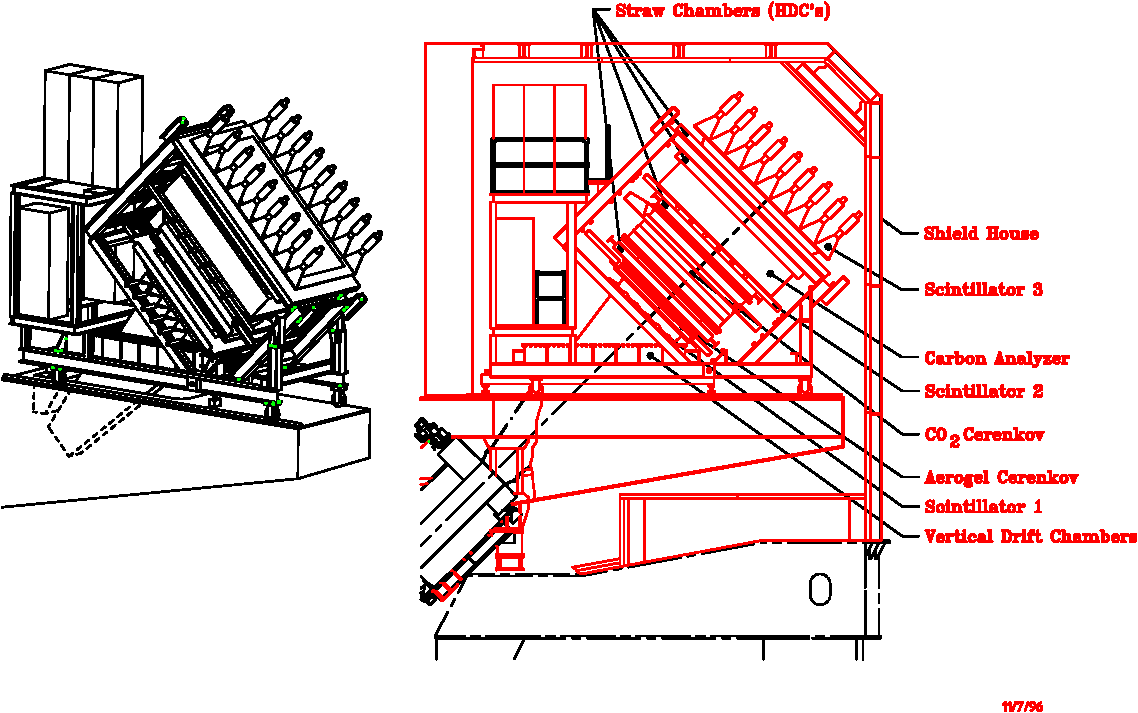
\includegraphics[angle=0,width=\textwidth,clip]{figure0104_r}
{\linespread{1.}
\caption[Spectrometers: Hadron Arm Detectors]{The hadron spectrometer detector stack.}
\label{fig:hrs_hadron_det}}
\end{center}
\end{figure}


The hadron detector is shown schematically in 
Figure~\ref{fig:hrs_hadron_det}.  It consists 
of two sets of (x,y) vertical drift wire chambers identical to those of the 
electron arm.  The remaining part of the detection system is used to 
define the level 1 trigger, as well as for particle identification and 
timing.  It consists of two minimally segmented planes of 
scintillation counters equipped with photomultipliers at both ends, and 
it includes \Cherenkov{} counters (gas CO$_2$ and Aerogel).

In addition, a proton polarimeter is installed in the back of the 
detector package to measure the polarization of the proton using a 
segmented carbon analyzer up to 60 cm in thickness to allow measurements 
over a wide range of proton energies.  A pair of front and a pair of 
rear straw tube wire chambers determine the incident and 
scattered angles, respectively.  The 
polarimeter detectors are dimensioned to accept a 20$^{\circ}$ cone of 
scattered protons.

Several support systems are necessary in addition to the basic 
components mentioned above.  They include gas supply systems for the 
wire chambers, high voltage supplies, readout electronics, a second 
level trigger, software for data analysis and testing, and a remotely 
controllable mechanical system.

For each spectrometer, all detectors are mounted on a 
single rigid support frame along with their associated electronics.  The trigger electronics are located on the support frame, next to the detectors.

To reduce the resolution degrading effects of multiple scattering, the 
entire interior of the spectrometer from the collimator box to the detector hut 
is a vacuum vessel.  The ends of this evacuated volume are capped by 
relatively thin vacuum windows.
}

\begin{safetyen}{0}{0}
\section{High Resolution Spectrometers}
\label{sec:hrs-safety}
\end{safetyen}

The principle concern with the spectrometers is that they are large, 
and have associated vacuum, hydraulic, cryogenic and magnet systems all of 
which can be potentially dangerous.

The bogies which move the massive 1200 ton spectrometers must be 
carefully operated.  Inspection of the floor and wheels to ensure there is no 
debris which the wheels could ride over is mandatory.  Similarly 
personnel need to be aware that the spectrometers are moving so that no one 
inadvertently gets trapped.

The vacuum systems associated with the spectrometers are essentially 
pressure vessels (see Chapter \ref{chap:vacuum} for more details).
Care should be exercised so as not to puncture the 
windows.

The magnets themselves are installed inside cryostats.  These vessels 
are exposed to high pressures and are therefore equipped with safety 
relief valves and burst discs.

The hydraulic system originally intended to operate the vertical positioning system (VPS) 
and the horizontal positioning system (HPS) has effectively been dismantled, after problems were encountered during the initial attempted operation of the system.

The cryogenic system operates at elevated pressure at 4K.  One must 
guard against cold burns and take the normal precautions with pressure 
vessels when operating this system.  Only authorized personnel are permitted to install 
and take out U tubes.

The magnets have a great deal of stored energy as they are large 
inductors. Always make sure people are clear of them and that
the dump resistor is attached to the magnet.

There are several major safety concerns with regards to the detectors, 
namely 1) flammable gas located in the VDC, 2) ODH hazard due to 
CO$_2$ in the \Cherenkov{} counter, 3) high voltage due to the photo 
multipliers on the various detectors and 4) a thin vacuum window 
separating the detector array from the vacuum system in the 
spectrometers.

\infolevltone{
\begin{safetyen}{5}{10}
For more information consult the full OSP manual~\cite{HallAosp}.
\end{safetyen}
} %infolev

\begin{safetyen}{10}{15}
\subsection{Authorized Personnel}
\end{safetyen}

In the event that problems arise during 
operation of the magnets, qualified personnel should be notified
(see Table \ref{tab:hrs:personnel}).  
This includes any prolonged or serious problem with the source of magnet 
cryogens (the ESR).  On weekends and after hours there will be a 
designated individual on call for magnet services.  Any member of the 
Hall A technical staff is qualified to deal with unusual magnet 
situations but in the event of serious problems the technician on
call should be contacted.

\begin{namestab}{tab:hrs:personnel}{HRS: authorized personnel}{%
      HRS: authorized personnel. ''W.B'' stands for the white board 
      in the counting house.}
   \TechonCall{\em Contact}
   \EdFolts{}
   \JackSegal{}
   \HeidiFansler{}
   \JessieButler{}
   \AndrewLumanog{}
   \JasonGlorioso{}
   \MahlonLong{}
\end{namestab}

\infolevone{
\section{The Magnets of HRS}

Each HRS is composed of three superconducting quadrupole magnets, Q1, Q2, 
and Q3, and one superconducting dipole magnet.  The large quadrupoles were 
manufactured for JLab by SIEMENS, the small quadrupole by SACLAY, while 
the dipole was built for JLab by WANG NMR.  The quadrupole magnets are 
referred to as Q1, Q2, and Q3, where a particle first traverses Q1, then 
Q2 and the dipole magnet and finally traverses Q3.

The magnet system is followed by a large steel and concrete detector 
hut, in which all detector elements reside.  Most of the 
detector elements have been built by universities involved in the Hall A 
physics program.

The HRS magnet system is the cornerstone of the Hall A activities.  
Many of the experiments approved in Hall A center on physics at high 
resolution and other short-range phenomena, and rely on a spectrometer 
able to momentum analyze charged particles up to very high momenta.  The 
design value for the maximum momentum accessible to the HRS magnet 
system is 4 GeV/c.
}

\subsection{Magnets and Power Supplies}

\infolevone{
The HRS magnet's are all superconducting and hence their coils must be 
maintained at cryogenic temperatures during operations.  The LHe 
required by the magnets is supplied by the End Station Refrigerator, ESR.

All the HRS magnets cryogenic services are supplied through the overhead 
cryogenic lines.  The distribution network begins at the distribution 
box over the pivot.  This box is connected to the rest of the network 
via the flexible transfer lines over the pivot.  The network is adjacent 
to the upstairs catwalk of the HRS.

Cryogenic information about each magnet is available on the control 
screens in the counting house, one for each magnet.  Normally during run 
periods the control screens are sent upstairs to the Hall A counting 
house and information on all the HRS magnets is available on the HRS 
control screen located in the center of the main console.  The control 
of all magnets is described in a following Section.

The power supplies for the magnets are located on the gantry balcony 
adjacent to the magnets.  The supplies are all cooled with low conductivity water (LCW).
}

\begin{safetyen}{10}{15}

Under no 
circumstances should any panel of any magnet power supply be opened by someone 
other than authorized personnel.  There are also 
signs posted listing the dangers of high magnetic fields.
\end{safetyen}

\infolevone{
A control interface for the power supplies is available through the 
HRS control screen in the Hall A counting house.
}

\infolevone{
\subsection{Quadrupole Magnets}

The quadrupoles provide some of the 
focusing properties of the spectrometer and to a large extent 
its acceptance.  Operating limits imposed on the 
quads are as follows: 1850A for Q2 and Q3 and 3250A 
for Q1.

All three quadrupoles for the HRS spectrometer are warm iron 
superconducting magnets.  The soft iron around the superconducting coil 
enhances the field at the coil center and reduces stray fields.  The 
basic parameters for the first quadrupole, Q1, are an effective length of about 
0.9 $m$, useful aperture of 0.3 $m$ and a field gradient of 9.5 
T/m.  To achieve the lowest possible angle setting of the HRS 
spectrometer (with respect to the beam line) the incident electron beam passes through
a notch in the outer yoke of Q1 when the spectrometer is at
its smallest angle of 12.5$^\circ$ . The 
other two quadrupoles, Q2 and Q3, are essentially identical with an 
effective (magnetic) length of about 1.8 meter, a useful aperture of 
0.6 $m$ and a field gradient of 3.5 T/m.
}

\infolevthree{
The maximum operating currents (assuming a 4 GeV/c momentum particle) 
for the quadrupoles are about 3000 A, 1700 A, and 1600 A, for Q1, Q2, and 
Q3, respectively.  This will render pole field values 
of 1.2, 1.0, and 1.0 T, respectively.  The energy stored in the 
quadrupole fields is sufficient to cause an unrecoverable quench if all 
the energy stored is dumped into the magnets.  Therefore a quench 
protection circuit is incorporated.  However, a quench can only happen 
if the cryomagnets have a helium level below the coil 60\% during operation.

The operating current to the Q1 quadrupole coils is provided by Danfysik 
System 8000 power supplies, which can operate up to 3500 A current and 5 
V.  The power supplies will be cooled with a combined maximum 
water flow of 45 liters per minute.

In addition to the main quadrupole windings, all quadrupoles have 
multipole windings.  To further optimize focusing properties of the HRS 
magnet system, it was intended to operate including some of these multipole 
trim coils in order to reduce higher order aberrations.
The operating current for these multipole corrections would be 
small, only (the multipole corrections are typically less than 2\% of 
the main quadrupole field), of order 50 A. Since the sextupoles were inadvertently 
installed rotated 90 $^\circ$ from their correct
orientation, these trim coils are now considered useless 
and there are at present no plans to use them.

\subsection{Cryogenic Procedures}

The cryogenics control is handled by the JLab Cryogenics Group.  The cryo control coordinator 
can be reached at the CHL (x7405) or by calling the MCC.

\subsection{First Time Startup Check List.}  

See attached check lists for all quadrupole and dipole magnets
 (Tables~\ref{tab:dip_check}, \ref{tab:q1_check}, and \ref{tab:q23_check}).
} %infolev

\infolevone{
\subsection{Dipole Magnet}

The dipole, by virtue of its field index, provides both
dispersion and focusing.  The present operations envelope 
states that the supply for the left HRS dipole may not be
operated at a current above 1800 A (4.4 GeV/c). The supply for the right HRS
dipole may not be operated above 1200 A (3.2 GeV/c), due to complications
caused by an internal short. 

The dipole for the HRS spectrometer is a superconducting, cryostable 
magnet.  Its basic parameters are an effective length of about 6.6 $m$, a 
bend radius of 8.4 $m$, and a gap width of 25 $cm$.  It is configured to 
achieve a 45 degree bending angle for 4 GeV/c momentum particles at a 
central field excitation of 1.6 T.  For the HRS dipole to reach 1.6 T 
an operating current of about 1500 A is required.
} %infolev

\infolevthree{
The dipole has been designed to achieve cryostability up to a field of 2 
T, and this property has been extensively tested up to a field of 1.6 T. 
 The cryostable coils are equipped with an energy removal circuit to 
cover the possibility of an unrecoverable quench.  However, this can 
only happen if the helium level drops below the coil during operation.  
The current to the coils will be provided by a Dynapower Corporation power 
supply, which can operate up to 2000 A and 10 V.  This 
power supply is located on the gantry beside the dipole, and will be 
cooled with a maximum water flow of 35 liters per minute.
The total water flow needed to cool the 4 power 
supplies for the HRS magnet system (dipole and quadrupoles) amounts to 
80 liters per minute, with a supply pressure of cooling water for Hall A 
of 100 psi.
} %infolev

\infolevtwo{
\section{Operation of the HRS Magnets}

\subsection{Introduction}

This is an abbreviated operating manual for 
the HRS superconducting magnets specifically designed for Hall A 
experimenters.  It provides instructions for setting currents, invoking 
NMR field regulation and general system monitoring.  Curious readers are 
directed to the references for more in-depth operating instructions and 
other technical manuals. Copies of the following supporting
documents are available in the Hall A Control Room and through the Hall A webpage
(see Table~\ref{tab:hrs-mag-manuals}).

\begin{table}[htp]
\begin{center}
\begin{tabular}{|l|l|}
\hline
References & \\
\hline 
WANG NMR Dipole & User Manual \\
Dynapower & Instruction Manual \\
Appendix & NMR Tesla meter \\
Appendix & NMR Field Regulation \\
Siemens/Fug & Q2/Q3 Magnet Instrumentation and Power Supplies \\
Saclay/Danfysik & Q1 Power Supply Manual \\
TOSP & HRS Dipole \\
TOSP & HRS Quadrupole Q1 \\
TOSP & HRS Quadrupole Q2, Q3 \\
HRS & SC Dipole Magnet Safety Review Vol. 2 \\
HRS & SC Quad Safety Review Vol. 1 \\ \hline
\end{tabular}
\end{center}
\caption[HRS Magnets: extra manuals]{HRS Magnets: extra manuals available in 
     Hall A Control Room.}
\label{tab:hrs-mag-manuals}
\end{table}

\subsection{Simple HRS Setting (Autopilot Mode)}
\label{sec:hrs-mag-set} 

 The magnets are controlled remotely using EPICS~\cite{EPICSwww} and
 EDM~\cite{EDMwww} GUI, provided that everything is working and power 
 supplies are turned on and ready to go.
 The appropriate interface runs
 on the computer \mycomp{hacsbc2} (see Section \ref{sec:contr-ha-menu}).
 On the ``Hall A General Tools'' control screen, in the upper left, there is 
 a rectangular box for each spectrometer (see Figure~\ref{fig:hrs_mag_cntrl}). 
\begin{figure}
\begin{center}
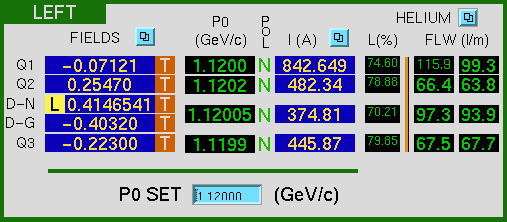
\includegraphics[angle=0,width=0.8\textwidth]{medm_halla_tools_1_cut1}
{\linespread{1.}
\caption[HRS: Magnets control]{A part of ``Hall A General Tools'' screen, 
        used for HRS (left) magnets control.}
\label{fig:hrs_mag_cntrl}}
\end{center}
\end{figure}

This box displays a brief summary of the status of the spectrometer
magnets and their cryogenic systems. The blue fields (with white
numbers) give readbacks of the magnetic fields and currents in each
magnet. The black fields also give readbacks, however in this case if
the text appears green those parameters are OK while if they are red
then that parameter is out of tolerance and may indicate a fault
condition. For example if the helium level goes below a certain point
the magnet will be automatically turned off.  In some cases it may be
desirable to monitor certain critical quantities on a strip chart
(e.g. magnet settings). A strip chart tool is available for this
purpose from the bottom of the ''EOS Menu'' button in the ''MyMenu'' window.

{\bf To set the spectrometers} for a given value of central momentum
(P0) type the desired P0 value into the light blue P0 SET box and hit
return. The magnets will be automatically 
set to the correct
values. All green numbers in the P0 column indicates that the desired
field or current settings have been reached. 

{\bf Caution:} Regarding the
dipoles, in general it's a bad idea to assume that at the first
instant that the P0 display turns green that the desired field has
been reached and you can start taking data. Stable field is in general
not achieved for from 15 to 30 minutes after reaching the nominal
desired field. This settling time depends on the magnet (the right dipole is
slower than the left dipole) and the magnitude of the field change (small
changes settle faster than big changes). Experimenters are advised to
observe both the field reading and current reading on the magnet in
question and verify that things are stable to their satisfaction
before proceeding.
 
\subsection{Powering Up Dipole Magnets:}

Use these instructions to recover from loss of a magnet due to a fault
(e.g. He level or lead flow fault). The order of actions matters. \\
(Contact Tech-On-Call if anything behaves funny or things don't
respond as expected. Sometimes after a trip an access to the Hall is
required to reset things).

\begin{list}{\arabic{enumi}.~}{\usecounter{enumi}\setlength{\itemsep}{-0.15cm}}
   \item Wait for Iout=0 (you can't and don't want to do anything while the magnet is in emergency fast dump mode.)
   \item While waiting, make a log entry re the fault. Give details such as time, coincident activities, and nature of the fault.
   \item Make sure the fault is cleared. (e.g. He level and flow rates returned to normal values and stable)
   \item In the HRS Right (Left) Dipole Systems' control panel:
   \begin{list}{}{\setlength{\itemsep}{-0.15cm}}
      \item[(a)] Press RESET (verify that all faults are cleared in the middle column)
      \item[(b)] Press ON (Display will indicate Power Supply ON and Magnet ENGAGED)
   \end{list}
\end{list}


Power supply and magnet are ready to go. From here you can return 
to "Autopilot Mode" (see Section \ref{sec:hrs-mag-set}).

\subsection{Starting Q1 Power Supply:}

 Do this when a fault causes the power supply to shut off.
 Wait for fault to clear (watch He levels). 
\begin{list}{\arabic{enumi}.~}{\usecounter{enumi}\setlength{\itemsep}{-0.15cm}}
   \item Push POWER OFF/RESET (check all faults cleared)
   \item Select desired polarity
   \item Push POWER ON
   \item Type in Setpoint (Amps) (light blue field) or re-enter P0 in Autopilot Mode.
\end{list}

\subsection{Starting Q2/3 Power Supply:}

 Do this when a fault causes the power supply to shut off.
 Wait for cause of fault to clear (watch He levels). 
 \begin{list}{\arabic{enumi}.~}{\usecounter{enumi}\setlength{\itemsep}{-0.15cm}}
   \item Push RESET 
   \item Select desired polarity
   \item Push ON
   \item Type in Current Set (light blue field) or re-enter P0 in Autopilot Mode.
\end{list}

} %infolev

\subsection{Rotation}
%
% Thanks to John LeRose for Rotation text. 07NOV2013
%
Moving an HRS
Since each HRS weighs in excess of 1,000 tons it is very important that all safety
precautions are carefully adhered to. The good news is they move very slowly (a few degrees/min
maximum), BUT 1,000 tons moving even very slowly is hard to stop. 

Hazards include:
\begin{itemize}
\item{Knocking items over.}
\item{The wheels crushing things (including fingers and toes) on the floor in the path of the 
spectrometer}
\item{Damaging the beamline or other equipment on the floor if one goes to too small 
or too large an angle, or if it just gets pushed around inadvertantly.}
\item{Tearing out of cables etc. physically attached to the superstructure}
\end{itemize}

Hazard mitigations:
\begin{itemize}
\item{Guards on either side of the wheels prevent items from getting under them.}
\item{Large pins in the floor to stop the spectrometer rotated beyond the needed angular range.}
\item{Blinking lights on the spectrometers indicating they are in motion or that motion
is possible (controls engaged etc.)}
\item{During a running experiment the run coordinator and work coordinator should know in advance 
of any moves.  Moves at any other time must be cleared with the Hall work coordinator 
before implementation.}
\item{Careful inspection of the intended path to make sure it is clear. This is part of
the pre-run checklist performed by the technical staff prior to closing the Hall and
a remote camera allows shift worker to inspect the area.}
%
%\item{Any motion that takes a spectrometer inside 14 degrees or outside x degrees
%(x being specified in the pre-run checklist and noted on the whiteboard during a run) 
%must be supervised by a trained Hall A technician.}
\end{itemize}

\infolevone{
Remote Procedure for a shift worker:
\begin{itemize}
\item{Make sure the move is part of the approved runplan (if in doubt, check with the 
run coordinator).}
\item{Check that the pre-run checklist has been completed and note and comply with any 
possible limitations to spectrometer motion (if there is a conflict inform the Run
Coordinator and do not initiate any move until the conflict is cleared).}
\item{Visually inspect the Hall using the closed circuit TV cameras to verify that there
are no obstructions.}
\item{If people are in the Hall wait until they leave (during a Controlled Access MCC keeps
track of people in the Hall). (Maybe we could soften this to "Inform EVERYONE in the Hall of
the move".)}
\item{Activate the spectrometer motion controls (see the Wiki and below) and 
move to the desired angle.}
\item{Deactivate the controls (brakes on, power off, etc.)}
\item{Update the spectrometer position information on the Hall A Controls screen}
\item{Make a halog entry indicating you've moved the spectrometer including from what angle 
to what new angle.}
\end{itemize}

Procedure for a non-run associated move in the Hall:
\begin{itemize}
\item{Inform the work coordinator of the planned move}
\item{Perform a careful visual inspection to verify that the path is clear}
\item{Check to make sure there are no temporary connections to the spectrometer (wires etc.)
that could be damaged during the move.}
\item{Inform everyone in the Hall of the move and check with them re 3.}
\item{Activate the spectrometer motion controls (see the Wiki and below) verify 
that the warning lights are on and move to the desired angle.}
\item{Deactivate the controls (brakes on, power off, etc.).}
\end{itemize}

The full proceedure for moving the spectrometer follows and can also be found on the Hall A wiki.

On hacsbc2, click the red "tool box" icon on the linux taskbar, as above. Choose 
bogies\_SetSpec so that you can determine the angle and vernier setting for the spectrometer.
Enter the spectrometer (L or R), and the angle, and you will get two options for the floor 
mark and the vernier. Generally choose the vernier closer to zero. Center the cameras on the 
desire vernier using the Move+/Move- buttons on the Hall A General Tools screen. The TV monitors 
for these cameras are on the middle shelf, in rack CH01A05.

Choose bogies\_Left (or bogies\_Right) in the tool box to bring up the bogies control screen. 
Click PSM enable and wait a few seconds for PSM OK to read YES. 
Click DM enable and wait a few seconds for DM OK to read YES.
Make sure the velocity is set to 0 and the direction is CW or CCW as desired. Click on Brake Release 
and wait for Brakes OK to read YES.

Click on ClampRelease, set the velocity to 700. Once you see the spectrometer start to move in the 
floor angle camera - you cannot see the spectrometer move in the Hall overview camera, as it only 
moves a few degrees per minute at maximum speed. For the left arm, to move to a larger angle, the 
direction should be CCW, while for the right arm CW moves the spectrometer to larger angle. The 
direction of the spectrometer is reversed by using a negative rpm. Watch the spectrometer motion 
on the cameras. When you are getting close to the desired angle, slow down to about 300 rpm. 
To stop, click on the Clamp Release button and the Brake button. Disable DM and PSM, and disconnect 
to close the GUI. Read off the floor angle mark and vernier, and input the values into the appropriate 
fields in the Alignment section of the Hall A General Tools GUI. 
}









\newpage
\section[Field Monitoring]{Field Monitoring
\footnote{
  $CVS~revision~ $Id: nmr-1999.tex,v 1.4 2003/12/17 03:59:48 gen Exp $ $ 
}
\footnote{Authors: J.LeRose \email{lerose@jlab.org}}
}

The field-monitoring controls are available using the main 
HRS screen%
\infolevtwo{ (see Figure~\ref{fig:hrs_mag_cntrl})%
}. % infolev
The dipoles' field is measured using NMR Teslameters and
field probes.

\infolevone{ 
 
\subsection{ Dipole Field Monitoring Electron Arm}

\noindent {\bf Basic Setup}

Each spectrometer dipole magnet is equipped with a Metrolab PT 4025 
NMR Teslameter, several field probes, and multiplexers (to allow switching 
between the probes).  Details of the operation and theory of operation 
for the Teslameter can be found in its user manual, 
a copy of which is available in the the counting house.
The basic layout is shown in Figure~\ref{fig:nmrbasic}


\begin{figure}
\begin{center}
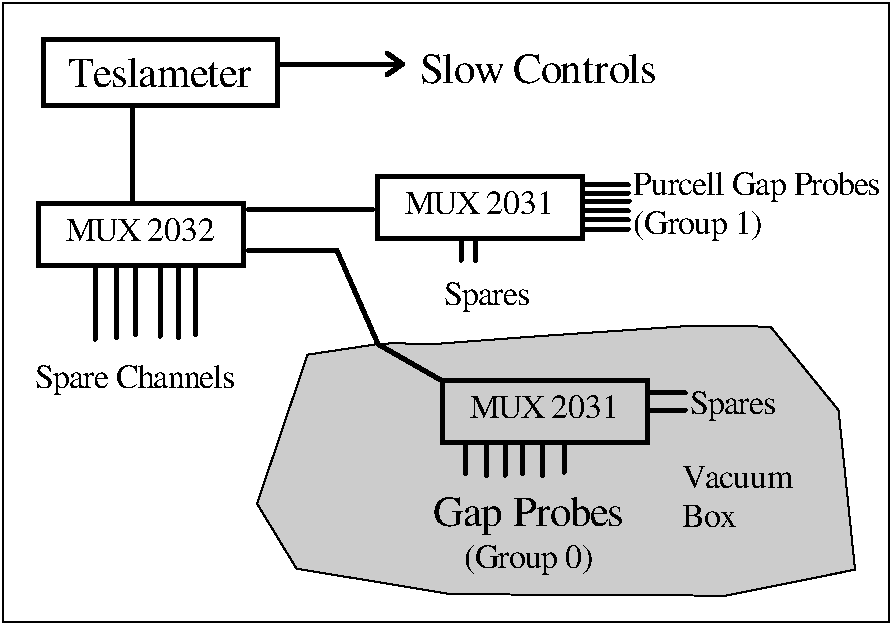
\includegraphics[angle=0,width=15cm,clip]{lerose_fig1}
{\linespread{1.}
\caption[Spectrometers: NMR System Layout]{Basic layout of NMR system}
\label{fig:nmrbasic}}
\end{center}
\end{figure}


 The "Gap Probes" (Group 0 in the controls) are located in two groups 
of three; one group on the low field side of the gap and the other on the high 
field side of the gap.  The groups of three are made up of one each of 
the manufacturer's type 3, 4 \& 5 probes, designed to cover different 
field ranges (see Table \ref{nmr_range}).  The six ``Purcell Gap Probes'' (Group 1 in 
the controls) are located in the Purcell gap of the magnet 
and consists of two each of the above types. {\em Note: Since
the fall of 1998 the multiplexer-multiplexer in both arms,
MUX 2032, has been removed and hence the ``Purcell Gap Probes'' are currently
unavailable. There are no plans to re-install this multiplexer.}

 The "Gap Probes" are equipped with coils which provide a field 
gradient that cancels out the field gradient of the magnet in the vicinity of 
the probe.  These gradient compensating coils are part of a simple circuit 
that is completely independent of the Teslameter.  The basic circuit for 
the compensating coils is shown in Figure~\ref{fig:nmrcir}


\begin{figure}
\begin{center}
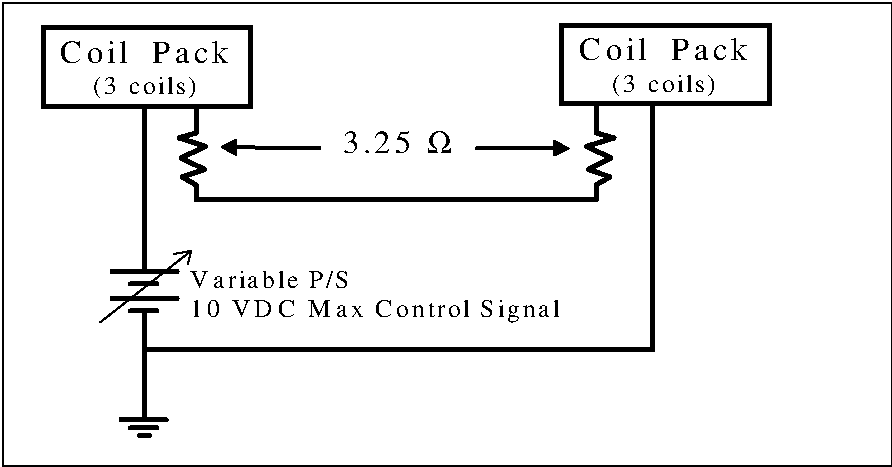
\includegraphics[angle=0,width=10cm,clip]{lerose_fig2}
{\linespread{1.}
\caption[Spectrometers: NMR Gradient Compensation]{Gradient Compensating Circuit.}
\label{fig:nmrcir}}
\end{center}
\end{figure}


%\snfig{figs/lerose_figcce.eps}{Control Voltage calibration for
%Electron Dipole }{nmrcomp4}{5in}

\begin{figure}
\begin{center}
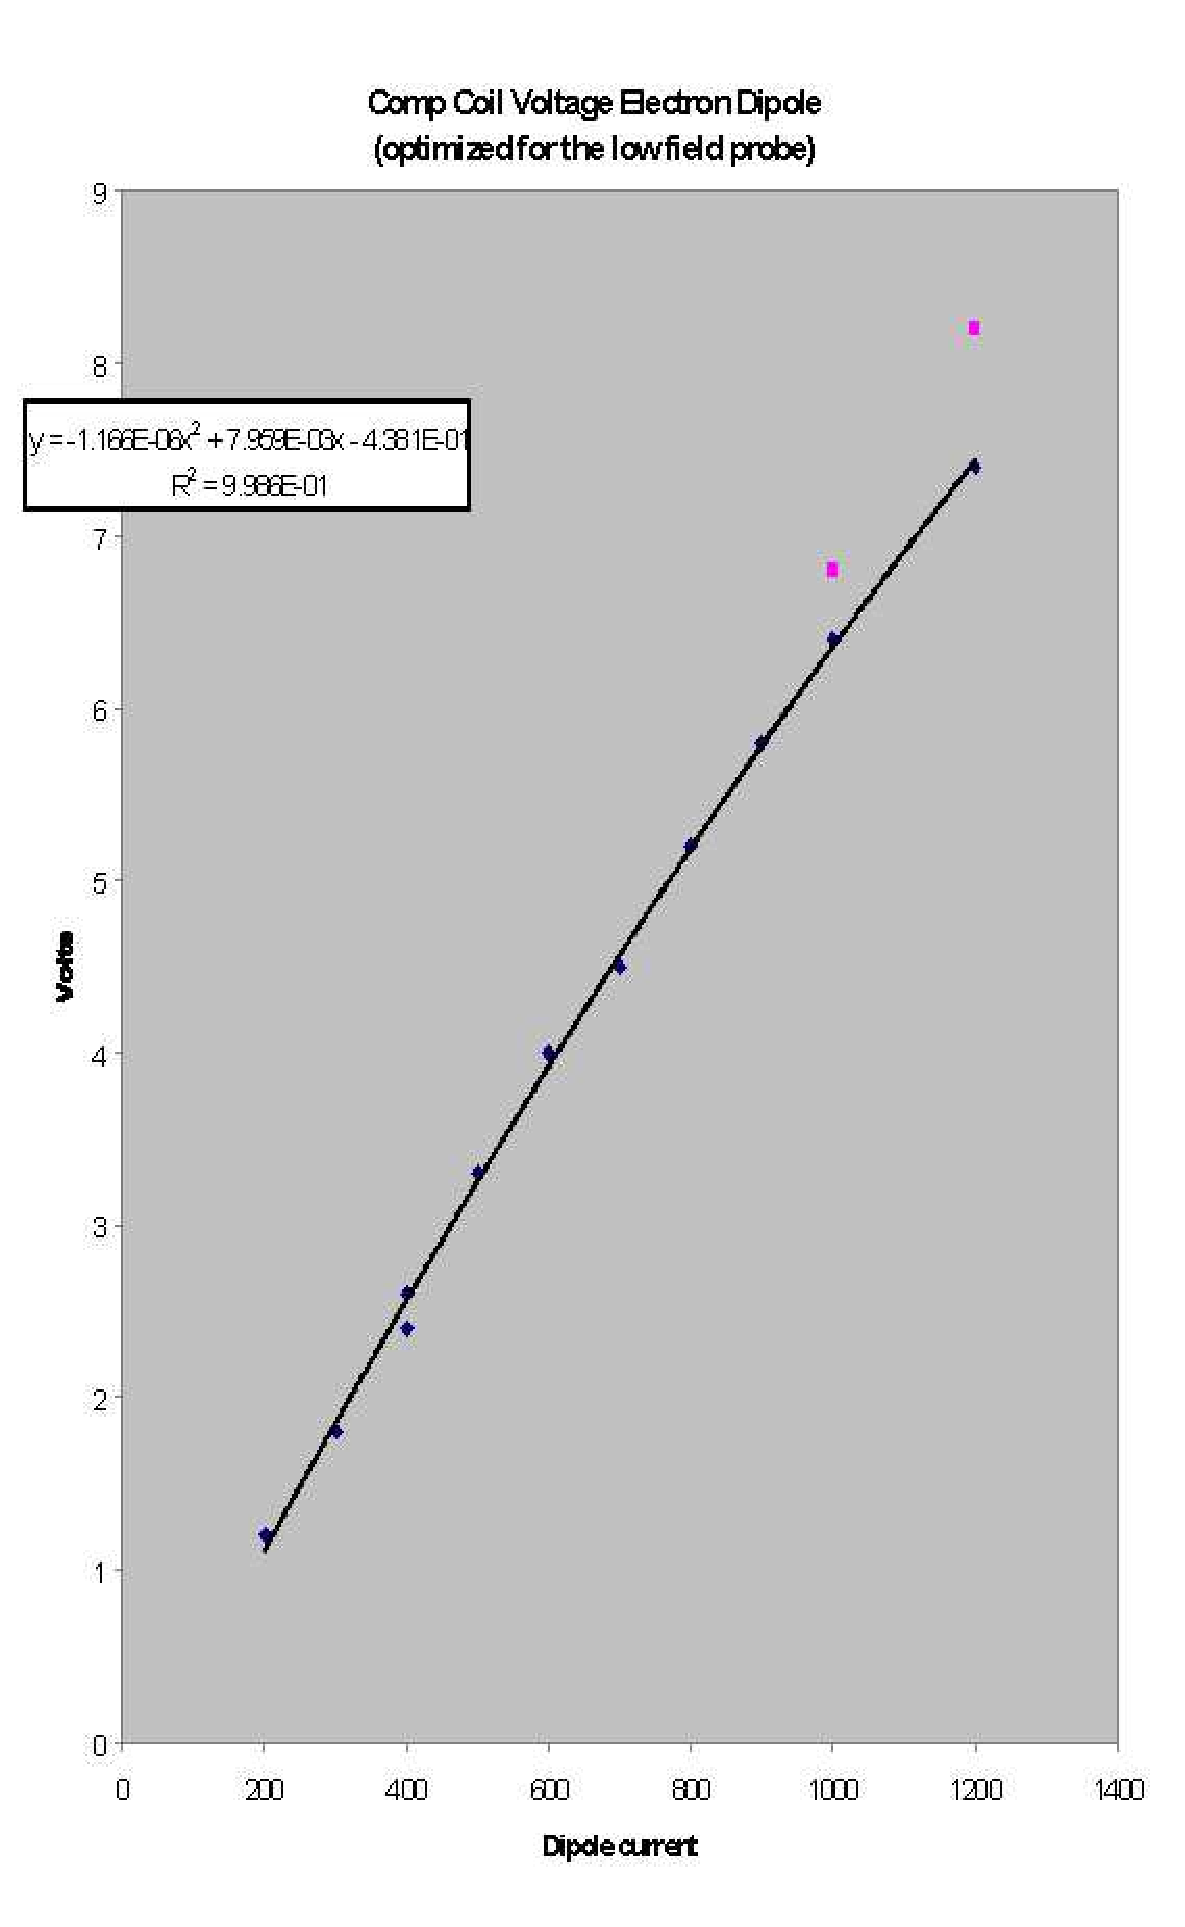
\includegraphics[angle=0,height=20cm,clip]{lerose_figcce}
{\linespread{1.}
\caption[Spectrometers: Control Voltage Calibration for Left Dipole]{Control Voltage calibration for the Left Dipole.}
\label{fig:nmrcomp4}}
\end{center}
\end{figure}

%\snfig{figs/lerose_figcch.eps}{Control Voltage calibration for
%Hadron Dipole }{nmrcomp5}{5in}
\begin{figure}
\begin{center}
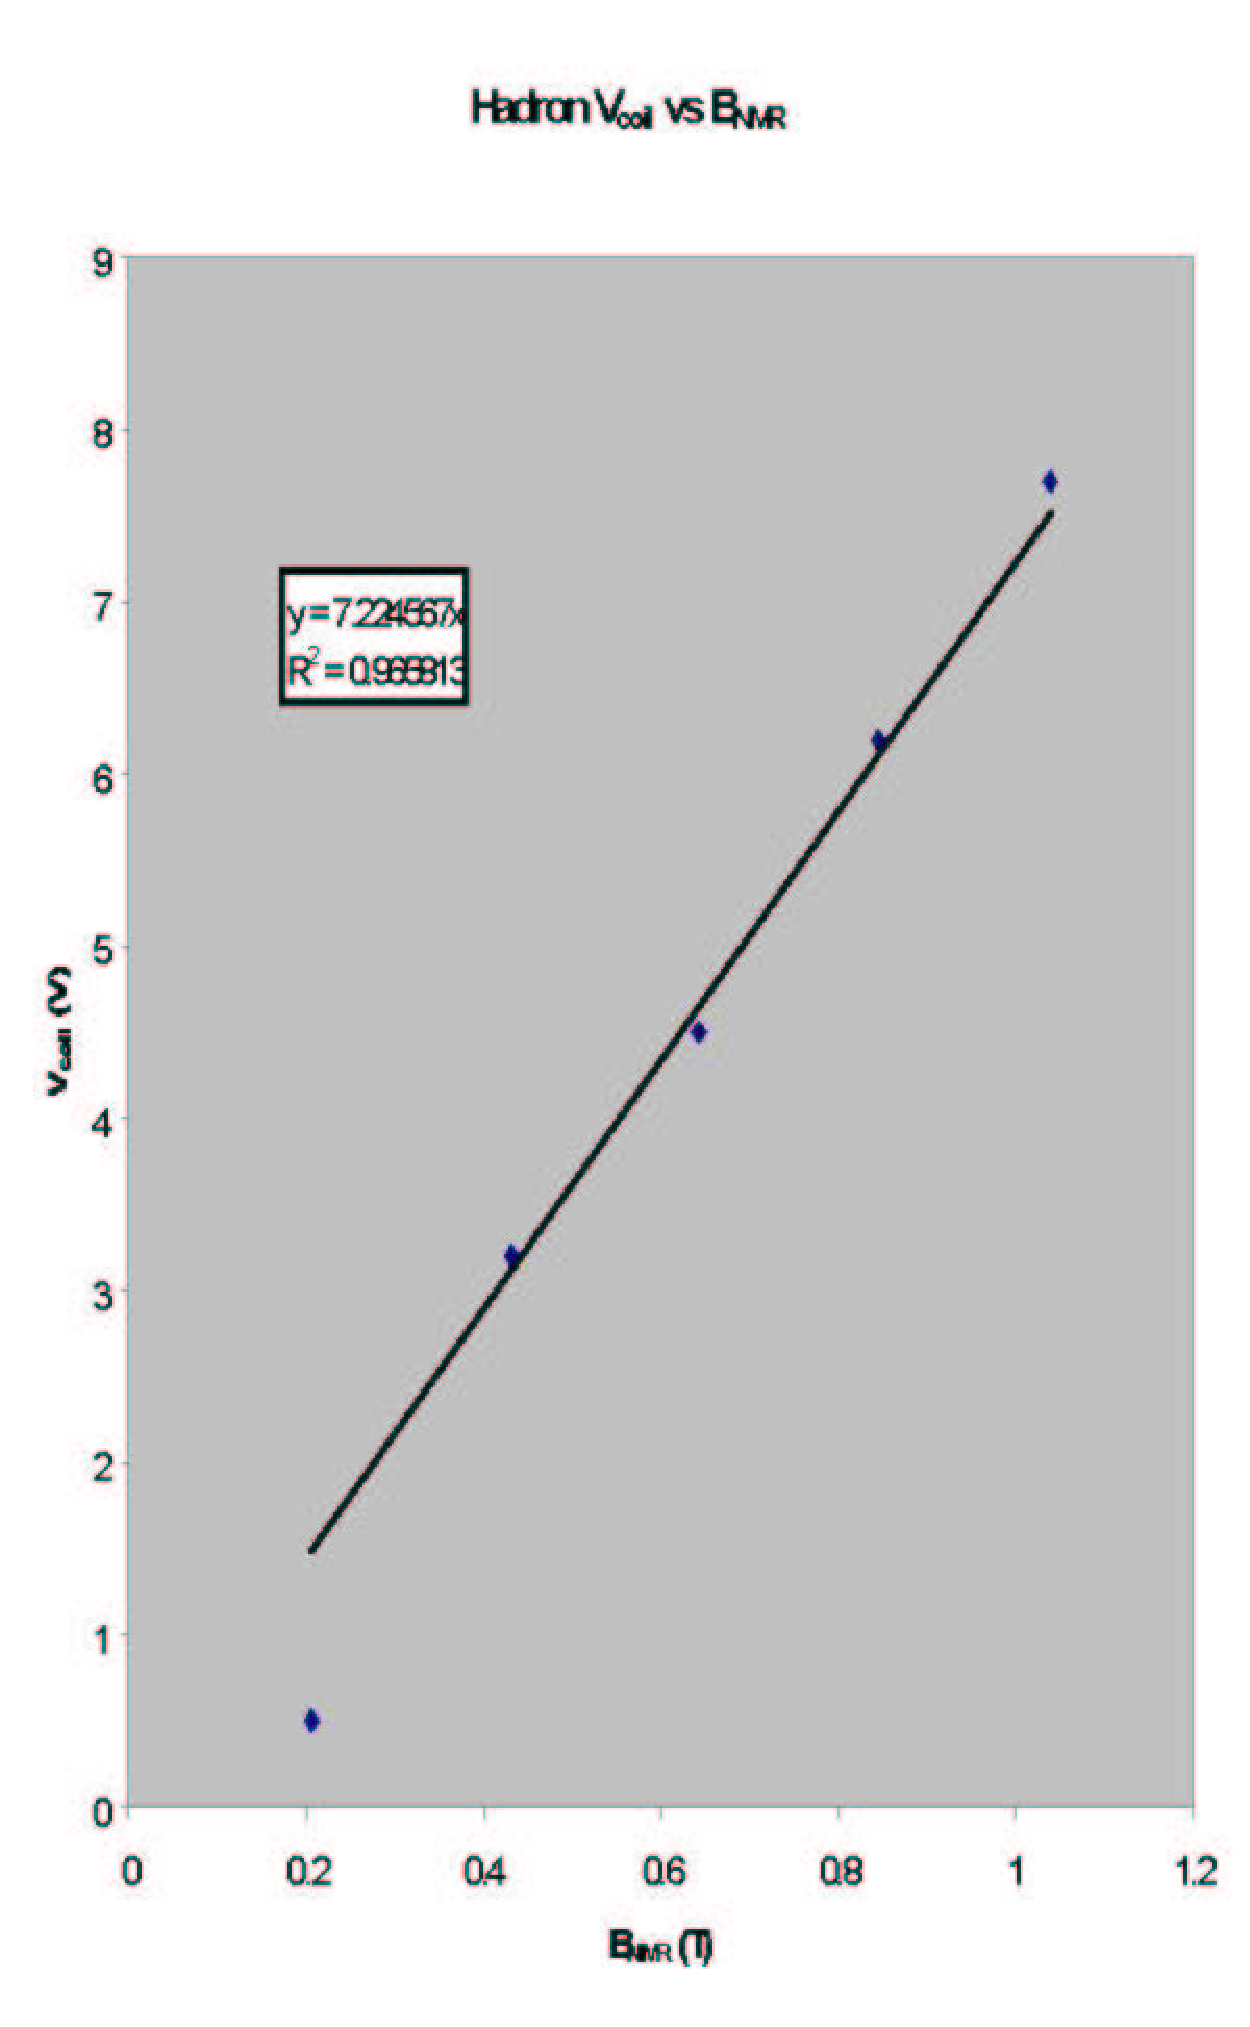
\includegraphics[angle=0,height=20cm,clip]{lerose_figcch}
{\linespread{1.}
\caption[Spectrometers: Control Voltage Calibration for Right Dipole] {Control Voltage calibration for the Right Dipole.}
\label{fig:nmrcomp5}}
\end{center}
\end{figure}

%\snfig{./figs/lerose_fig7.eps}{DAC Calibration for manual operation of NMR probes}{nmr_dac}{9in}
\begin{figure}
\begin{center}
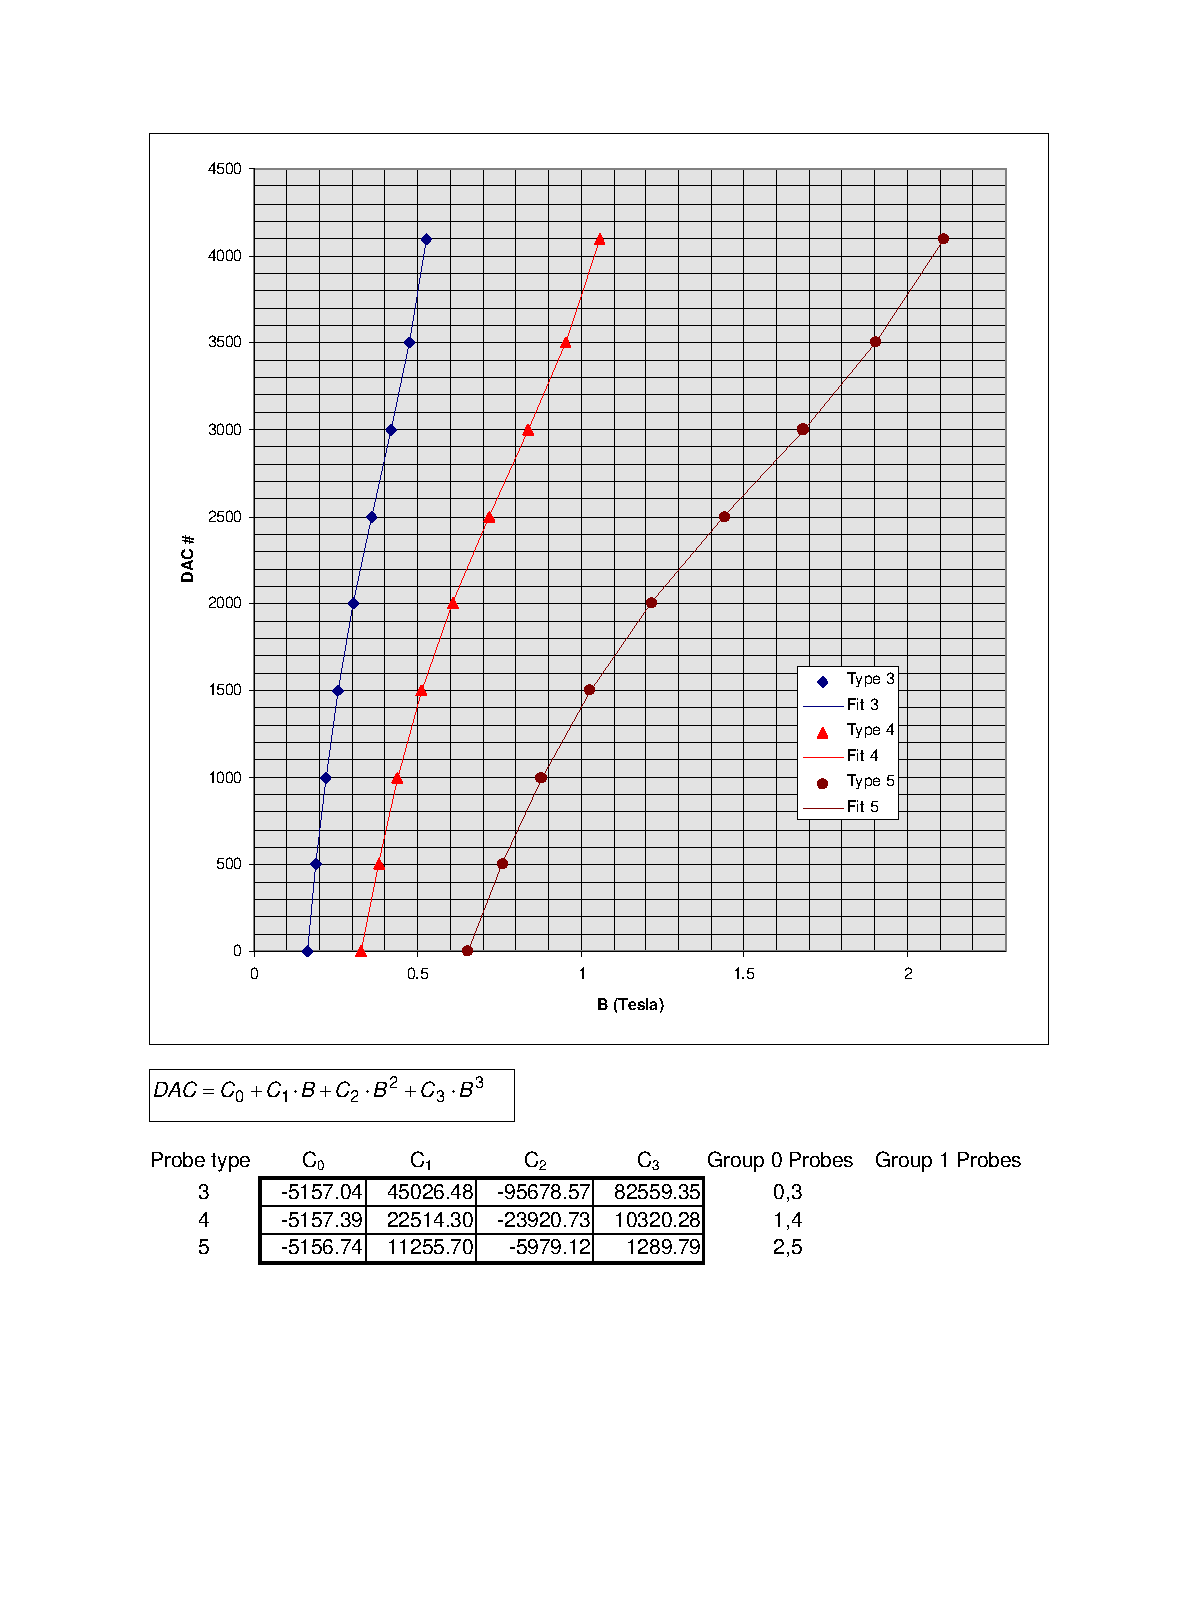
\includegraphics[angle=0,height=20cm,clip]{lerose_fig7}
{\linespread{1.}
\caption[Spectrometers: NMR Probe DAC Calibration]{DAC Calibration for manual operation of NMR probes.}
\label{fig:nmr_dac}}
\end{center}
\end{figure}

The following graphs (see Figures~\ref{fig:nmrcomp4} 
and ~\ref{fig:nmrcomp5}),can be used to determine optimum values for the 
compensating coil control voltage.  It should be noted that the setting 
of the compensating coil current is not very critical in most cases.  In 
general if you're within 10\% of the correct value everything should 
work fine.



\begin{table}
\begin{center}
\begin{tabular}{|cc|} \hline
Probe Type & Field Range (T) \\ \hline 
3 & 0.17 - 0.52 \\
4 & 0.35 - 1.05 \\
5 & 0.70 - 2.10 \\ \hline
\end{tabular}
\caption[Spectrometers: Dipole NMR Probe Field Ranges]{Dipole NMR probe field ranges}
\label{nmr_range}
\end{center}
\end{table}

} %infolev

\infolevtwo{
\subsection{NMR Operating Procedure}

When running in Autopilot mode (see: Simple Spectrometer Field Setting) the 
compensating coil voltage is set automatically and the probe appropriate for 
the field desired is selected. The gaussmeter is placed in SEARCH Mode and the 
dipole power supply software regulator is turned on. In this case the dipole current is 
adjusted to achieve the desired field. The user should just stand 
back and let it work. What follows are instructions for using
the NMR gaussmeter in situations where Autopilot doesn't work or
some special supplemental measurements are required. 

 In principle it is possible to make the field measurements using the 
SEARCH mode in the Teslameter.  In this mode you select a probe and the 
meter explores the whole field range of the probe until it finds and 
"locks" on the resonant signal indicating that it has a field 
measurement.  A ``lock" is indicated on the controls display by an ``L'' to 
the left of the field values.  This has the advantage of simplicity but in practice can 
be time consuming and doesn't always work.  The problem being, in 
situations where there is a lot of noise mixed in with the signal, the 
circuitry has problems distinguishing the signal from the noise and gets 
lost before it ever finds a lock.  The problem is exacerbated when the 
field being measured is at the high end of the probe's range.  In this 
case the search starts at the low end and keeps getting hung up on the 
noise and never gets to the field range of interest.  The solution to 
this problem is to tell the device approximately what field it's looking 
for and use the AUTO mode to find the lock.  In the procedure below that 
is what we will be doing.

In any case, for ``gap probes" (group 0) you must energize and adjust 
the gradient compensating coils for the field ranges to be measured before 
trying to make a measurement.

For studies involving 
10\% changes in the field settings the compensating coil current can be 
set once and left alone.


\noindent\underline{\bf Recommended Procedure:}(turn the {\bf SOFTWARE REGULATOR OFF} for all 
non-autopilot field measurements)\\
For group 0 probes set compensating coils appropriately (see figures).\\
Put the meter in MANUAL mode with SEARCH OFF \\
Select a probe \underline{\bf and} polarity (\underline{\bf Group 0:  
Probes 0, 1, 2 negative; Probes 3, 4, 5 positive}) \\
Type in the appropriate DAC number for the field range being measured (see below) \\
Select AUTO and wait for a lock (indicating a valid field reading) \\
Verify that you have a good lock by checking the oscilloscope for a 
clear resonant signal. \\
If you have problems see the table listing problems and possible 
solutions.

\noindent\underline{\bf Selecting DAC Number}

In selecting the DAC number to use for the field of interest use 
either the graph in Figure~\ref{fig:nmr_dac} or the polynomial at the bottom of the same figure.

\pagebreak
\noindent{\bf Problems and Solutions}\\
\begin{table}[htb]
\begin{tabular}{|p{0.4\textwidth}|p{0.55\textwidth}|}\hline
Symptom & Diagnosis and Cure \\ \hline\hline
Weird numbers on displays, controls for all magnets fouled up 
& Need to reboot.  See instructions below. \\ \hline
NMR Teslameter does not respond to commands and display shows all zeros. 
& Meter's communications are somehow hung up. Push {\bf RESET}. \\ \hline
%Will not lock & Very high noise level makes resonance hard to find. \\
%Still 
Will not lock 
& Very high noise level makes resonance hard to find. Search for the resonance manually by 
  adjusting the DAC in manual mode until you see the resonant signal.  (It helps if you know 
  what field you expect so you'll know where to look). \\ \hline
You find resonance manually but still can't get a lock 
& Check probe polarity. Try decreasing and increasing DAC number by 1. Optimize signal 
  by adjusting compensating coils. \\ \hline
Can't find resonance manually 
& Try a different probe.  Use readings from other probes to tell you where to look for 
 the resonance with the probe that's giving you trouble.  Make sure
 compensating coils are energized properly.  Make sure magnet is on. \\ \hline\hline
\end{tabular}
\caption[NMR: Problems and solutions]{NMR: Problems and solutions}
\label{tab:nmr-problems-solutions}
\end{table}

\begin{table}[ht]
\begin{center}
\begin{tabular}{|p{0.3\textwidth}|p{0.3\textwidth}|p{0.3\textwidth}|}\hline
Problems & Explanation & Action \\ \hline
NMR not locked but current is changing in the right direction 
& Normal operation for large field changes  
& Wait. (see above) \\ \hline
NMR locked but current going in the wrong direction.
& Normal operation. 
& Wait. \\ \hline
NMR locked but field not correct and current not changing 
& Field regulation is disabled or software is confused.
& Check that field regulation is enabled. Enter desired field value or one
  very near the desired value again. \\ \hline
NMR field display freezes. (Usually but not always shows  -\#.0000000)
& NMR Gaussmeter is not communicating with software.
& Push {\bf RESET}. \\ \hline
\end{tabular}
\end{center}
\caption[NMR troubleshhoting]{NMR troubleshooting
}
\label{tab:hrs_nmr_2}
\end{table}

} %infolev

\begin{safetyen}{10}{15}
\subsection{Authorized Personnel}
\end{safetyen}

The individuals shown in Table \ref{tab:nmr:personnel} are responsible for NMR operation problems.

\begin{namestab}{tab:nmr:personnel}{NMR: authorized personnel}{%
      NMR: authorized personnel.}
  \JavierGomez{\em Contact}
  \JohnLeRose{}
\end{namestab}



\newpage
\section[Collimators and Sieve Slits]{Collimators and Sieve Slits
\footnote{
  $CVS~revision~ $Id: slit.tex,v 1.5 2003/12/13 06:23:38 gen Exp $ $ 
}
\footnote{Authors: J.LeRose \email{lerose@jlab.org}}
}

Both spectrometers have front-end devices for calibrating the optical
properties of the spectrometers. These are known as the collimator boxes.
These boxes are positioned between the scattering chamber and the 
first quadrupoles (Q1). Each box is carefully aligned and rigidly attached
to the  entrance flange of the Q1 of the respective spectrometer.  The boxes are
part of the vacuum system of the spectrometer.
In the septum configuration sieve slits and collimators are installed and removed manually.

Inside each box a ladder is mounted which is guided by a linear bearing
and moved up and down by a ball screw. On this ladder 3 positions are 
available to insert collimators. Below this ladder
a special valve is mounted that can isolate the vacuum in the spectrometer
from the target system. This valve should be activated when it is moved
in front of the holes connecting the box with spectrometer and target chamber.
\infolevone{
A schematic view of the collimator box is shown in Fig.~\ref{fig:coll}.

\begin{figure}
\begin{center}
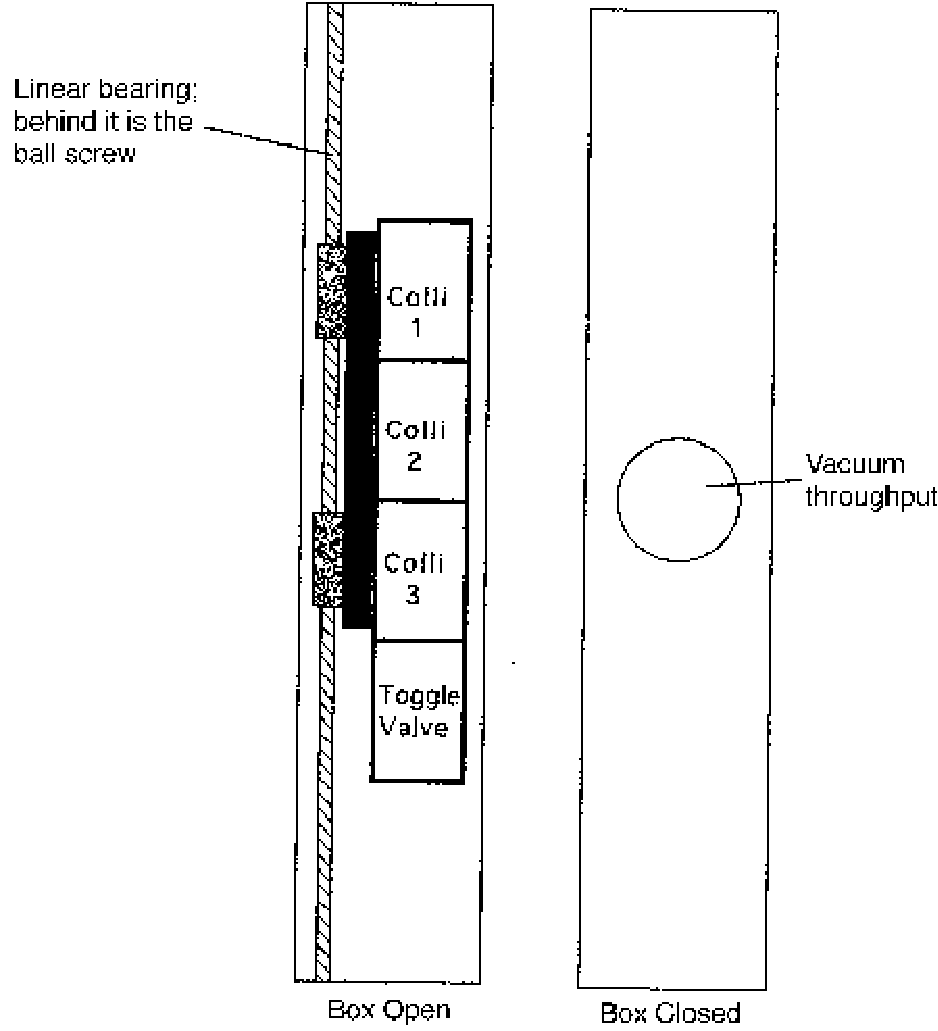
\includegraphics[angle=0,width=13cm,clip]{collimator_clip}
{\linespread{1.}
\caption[Spectrometers: Collimator Box Schematic]{Schematic layout of the collimator box.}
\label{fig:coll}}
\end{center}
\end{figure}
} %infolev

Vacuum requirement is $10^{-6}$ Torr. The material for the box is 
aluminum. It is possible to open one side of the box so that
collimators can be exchanged. The
reproducibility of collimator positions after moving
the ladder and/or after replacing a collimator is
better than 0.1 mm in horizontal and vertical direction.
The dimensions of the box are
roughly height=175 cm , width=35 cm and depth=15 cm.
The tolerance in the dimension
of the 7 msr collimator hole is $\pm0.5$ mm in each direction. 
The tolerance in the position
of each of the sieve-slit holes is $\pm0.1$ mm in each direction.

\infolevone{
\begin{figure}
\begin{center}
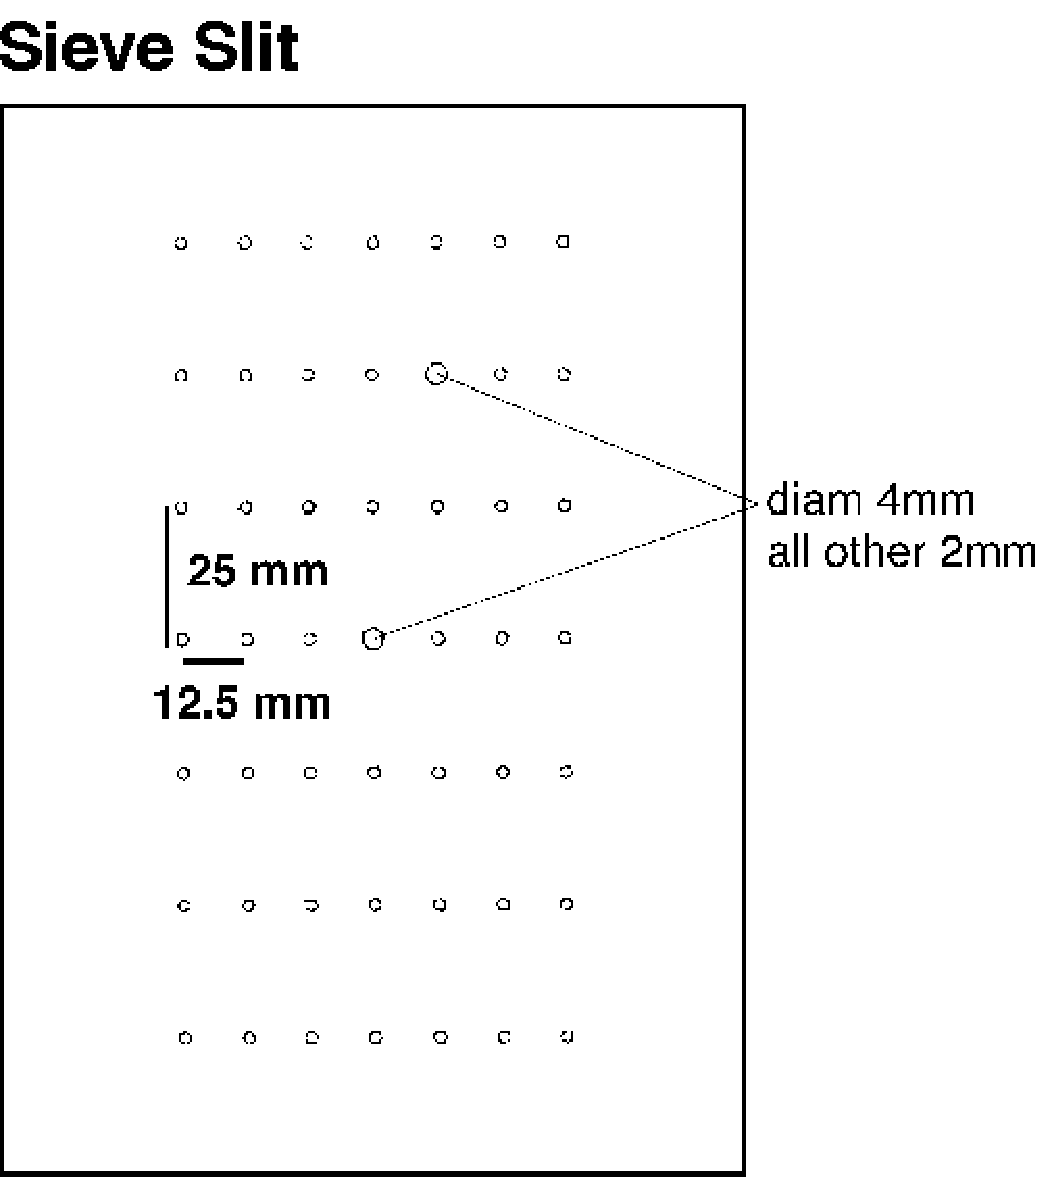
\includegraphics[angle=0,width=13cm,clip]{sieveslit}
{\linespread{1.}
\caption[Spectrometers: Sieve Slit]{Sieve slit collimator for optics calibration.}
\label{fig:sieve}}
\end{center}
\end{figure}
} %infolev
A typical sieve slit collimator 
\infolevone{(shown in Fig.~\ref{fig:sieve})
} %infolev 
consists of a plate of roughly 14 cm x 20 cm containing 49 holes
positioned in a regular 7x7 pattern. This slit is made out of 5
mm thick tungsten.
The holes have a diameter of 2 mm except for the central one and one positioned
off-diagonal which have a diameter of 4 mm. The horizontal distance between the
holes is 12.5 mm while the vertical distance is 25.0 mm.
%
%To get the latest information on the dimensions and locations of the collimators see 
%the Hall A homepage on the web%
%\htmladdnormallinkfoot{}{\url{
%http://hallaweb.jlab.org/
%}}.

To get the latest information on the dimensions and locations of the collimators see 
the Hall A homepage on the web%
\htmladdnormallinkfoot{}{\url{
http://hallaweb.jlab.org/
}}.

\begin{safetyen}{10}{15}
\subsection{Safety Assessment}

The collimator boxes form part of the vacuum system for each spectrometer. All hazards
identified in section spectrometer vacuum section applies to the collimator box as well.

In addition, safe access to the top of
the collimator boxes is needed  during manual operation of the box as outlined below.
Due to the proximity of the collimator boxes to the scattering chamber, and Q1 quadrupoles,
all necessary safety precautions with regards to vacuum windows, electrical power cables, 
cryogenic transfer lines, and high magnetic field should be taken. The same precautions also apply 
to the collimators and sieves in the septum configuration. In that case the sieve and collomators
can be considered part of the beamline. A survey and
appropriate RADCON designated proceedures must be followed when dealing with septum sieves 
and collimators.
\end{safetyen}

\infolevtwo{
\subsection{Operating Procedure}
Slit position is changed remotely from the standard Hall A control screen.
In the case of a spectrometer configuration involving the septum magnets collimators and sieves are
changed manually in the Hall.
} %infolev

\subsection{Authorized  Personnel} 

\begin{itemize} 
\item[~]E. Folts - x7857 (mechanical and vacuum systems).
\item[~]J. Gomez - x7498 (computer controls and electrical systems).
\end{itemize} 

% ===========  CVS info
% $Header: /group/halla/analysis/cvs/tex/osp/src/hrs/slit.tex,v 1.5 2003/12/13 06:23:38 gen Exp $
% $Id: slit.tex,v 1.5 2003/12/13 06:23:38 gen Exp $
% $Author: gen $
% $Date: 2003/12/13 06:23:38 $
% $Name:  $
% $Locker:  $
% $Log: slit.tex,v $
% Revision 1.5  2003/12/13 06:23:38  gen
% Septum added. Name tables. Polishing
%
% Revision 1.4  2003/12/05 06:49:07  gen
% infolevels added, polishing
%
% Revision 1.3  2003/06/06 16:13:37  gen
% Revision printout changed
%
% Revision 1.2  2003/06/05 23:30:00  gen
% Revision ID is printed in TeX
%
% Revision 1.1.1.1  2003/06/05 17:28:31  gen
% Imported from /home/gen/tex/OSP
%
%  Revision parameters to appear on the output

\newpage
\infolevtwo{
\section[Spectrometer Alignment]{Spectrometer Alignment
\footnote{
  $CVS~revision~ $Id: AlignmentOps.tex,v 1.8 2003/12/17 03:59:48 gen Exp $ $ 
}
\footnote{Authors: J.Gomez \email{gomez@jlab.org}}
}

At present, the systems implemented to determine the alignment of each spectrometer
(roll, vertical angle/pointing and horizontal angle/pointing) without the help of the
Accelerator Division Survey group are limited to roll, vertical angle and horizontal angle.
All alignment information is displayed in the ``ALIGNMENT'' mosaic of the ``Hall A
General Tools'' EDM screen%
\infolevtwo{ (see Fig.~\ref{fig:medm-hlamain-tools})}
(``EOS Menu'' $-->$ ``EDM (HLA Main)'' $-->$ ``Hall A Main Menu'' $-->$ ``Tools'').

A bi-axial inclinometer is used to determine the roll and vertical angle (also known as pitch)
of each spectrometer. These inclinometers are attached to the back of the dipoles at the power
supply platform level. The raw inclinometer measurements, in Volts,
are displayed as ``Tilt X'' and ``Tilt Y''. The inclinometer temperature is also given
(`` Tilt T''), in degree Celsius. From these values, the ``ROLL'' and ``PITCH'' values are
calculated.
Agreement between the inclinometer readings and survey measurements
are better than $\pm$ 0.1 mrad over all presently available history.

The horizontal spectrometer angle is determined from floor marks set in
place by the survey group. Floor marks have been placed every 0.5 $^\circ$ covering the useful range of
both spectrometers.
There are two concentric rings of floor marks in the hall. We will concentrate in the
inner ring which covers the angular range of both spectrometers. The outer ring is
similar.
The inner-ring floor marks are located at a distance of $\sim$10 $m$ from the target center.
A ruler attached to each spectrometer dipole runs over the floor marks and it acts as a vernier to interpolate
between marks. The location of a given floor mark on the ruler can be viewed from the Hall A Counting
House through a TV camera (labeled ``Front Camera'') .
The camera is able to move along the length of the ruler so that any
parallax effect can be eliminated. The camera motion is controlled from the ``Tools'' screen
through two push buttons (``FRONT CAMERA'' - ``MOVE +'' and ``MOVE --'').
Two fields in the ``ALIGNMENT'' mosaic
(``Flr Mrk'' and ``Vernier'') allow to input
the values read from the TV monitor. The effective spectrometer angle is then calculated and displayed
as ``Angle''. The application ``HRS Floor Marks'' calculates the floor mark and vernier value
to which the spectrometer should be set
to obtain a given angle. Spectrometer horizontal angle surveys and floor mark determinations
agree to $\pm$ 0.2 mrad.

\newpage
\begin{safetyen}{10}{15}
\subsection{Authorized  Personnel} 
\end{safetyen}
The authorized personnel is shown in table \ref{tab:align:personnel}.
\begin{namestab}{tab:align:personnel}{HRS alignment: authorized personnel}{%
      HRS alignment: authorized personnel.}
  \JessieButler{\em Contact}
\end{namestab}

} %infolev


% ===========  CVS info
% $Header: /group/halla/analysis/cvs/tex/osp/src/hrs/all.tex,v 1.3 2003/06/06 15:44:08 gen Exp $
% $Id: all.tex,v 1.3 2003/06/06 15:44:08 gen Exp $
% $Author: gen $
% $Date: 2003/06/06 15:44:08 $
% $Name:  $
% $Locker:  $
% $Log: all.tex,v $
% Revision 1.3  2003/06/06 15:44:08  gen
% Revision printout changed
%
% Revision 1.2  2003/06/05 23:30:00  gen
% Revision ID is printed in TeX
%
% Revision 1.1.1.1  2003/06/05 17:28:31  gen
% Imported from /home/gen/tex/OSP
%
%  Revision parameters to appear on the output

\chapter{High Resolution Spectrometers (HRS)}
\graphicspath{{hrs/figs/}}
\renewcommand{\dirfig}[0]{hrs/figs}
\renewcommand{\dircur}[0]{hrs}

\infolevone{
\chapter[High Resolution Spectrometers (HRS)]{High Resolution Spectrometers (HRS)
}
\footnote{Authors: J.LeRose \email{lerose@jlab.org}}
}
\label{chap:hrs}

\infolevone{
\section{Overview}
   
The Hall A spectrometers and associated instrumentation are designed to 
perform high resolution and high accuracy experiments.  The goal is to 
achieve a missing mass resolution of $\sim$ 200-500 keV to clearly 
identify the nuclear final state.  An absolute accuracy of $\sim$ 1\% is 
also required by the physics program planned in the Hall, which implies 
$\sim$ 10$^{-4}$ accuracy in the determination of particle momenta and 
$\sim$ 0.1 mr in the knowledge of the scattering angle.

The instruments needed are a high resolution electron spectrometer 
(HRES) and a high resolution hadron spectrometer (HRHS), both with a 
large angular and momentum acceptance.

\begin{figure}[tbp]
\begin{center}
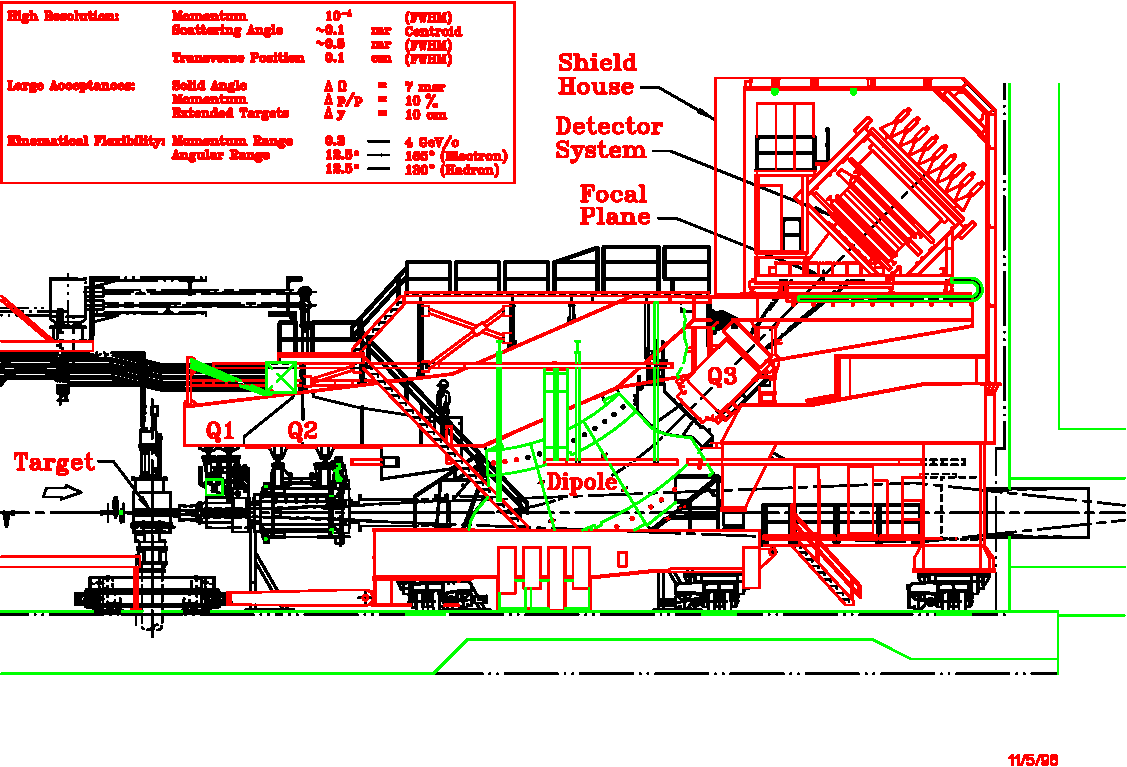
\includegraphics[angle=0,width=0.9\textwidth,clip]{figure0101_r}
\caption[Spectrometers: Elevation View of Hall~A HRS]{A side view of the Hall~A
HRS spectrometer.}  
\label{fig:hrs_ev}
\end{center}
\end{figure}
 
\begin{figure}[tbp]
\begin{center}
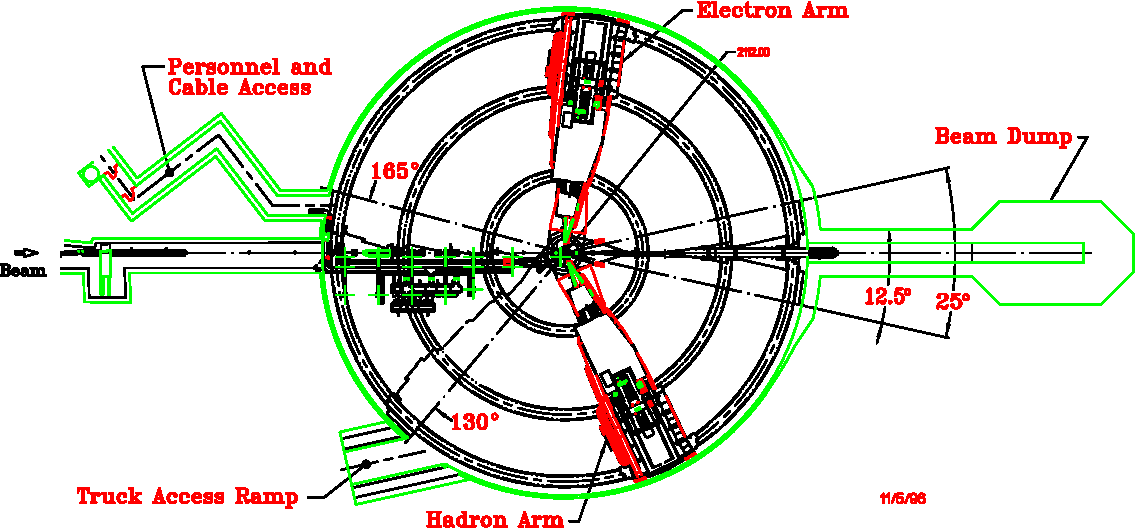
\includegraphics[angle=0,width=0.9\textwidth,clip]{figure0102_r}
\caption[Spectrometers: Plan View of Hall~A]{A bird's eye view of the Hall~A
end-station at TJNAF.}  
\label{fig:hrs_pv}
\end{center}
\end{figure}


A layout of the 4 GeV/c High Resolution Electron Spectrometer is shown 
on Figures~\ref{fig:hrs_pv} and \ref{fig:hrs_ev}.
Its main design characteristics are 
given in the attached table.  The spectrometer has a vertical bending 
plane and 45$^{\circ}$ bending angle.  The QQDQ design includes four 
independent superconducting magnets, three current-dominated 
cos2$\theta $ quadrupoles and one iron-dominated dipole with 
superconducting racetrack coils.  The second and third quadrupoles of 
each spectrometer have sufficiently similar field requirements that they 
are of identical design and construction.  The overall optical length, 
from target to focal plane, is 23.4 m.  Optically, the HRHS 
is essentially identical to HRES. In fact the two spectrometers can be used 
interchangeably to detect either positively or negatively charged particles 
as needed by any particular experiment. They are now commonly refered to 
as ``The Left Arm'' and ``The Right Arms'' rather than ``Hadron'' and ``Electron'' 

The support structure includes all system elements which bear the weight 
of the various spectrometer components and preserve their spatial 
relationship as required for 45$^{\circ}$ vertical bending optics.

The alignment and positioning system includes all the elements which 
measure and adjust the spatial relationship.  The support structure 
consists of the fabricated steel components which support the magnets, 
detector, shield house and associated equipment.  It is composed of the 
box beam, which supports the outer elements in fixed relative position 
atop the dipole; the dipole support bracket, upon which the dipole rests on 
the jacks; the cradle, upon which the dipole rests through the vertical 
positioning system, VPS; and a portion of the shield house load through 
the inboard legs of the gantry; the gantry, which supports the shield 
house and the magnet power supplies; and the bogies, which support the 
cradle-gantry assembly and roll on the floor plates and provide the 
driving power to move the two spectrometer arms.

The detector package (described in detail in Chapter \ref{chap:hrs-det})
is supported on the box beam and is surrounded by 
the shield house.  It must perform two functions, tracking and particle 
identification, PID.  The most important capability of focusing 
spectrometers is measuring precisely the momenta and entrance 
orientations of the tracks.  Momentum resolution of 10$^{-4}$ is 
obtainable, consistent with the resolution of the incident beam.

The actual configuration of the detector package varies from experiment to
experiment. The description given here is only an example of what is possible.
}

\infolevone{
A particle traversing the detector stack 
(Figure~\ref{fig:hrs_electron_det}) encounters two sets of horizontally
mounted, vertical drift wire chambers (x,y) with two planes of 368
wires in each chamber. The track resolution is $\sim$ 100 $\mu$m.  
From the chamber information both 
positions and angles in the dispersive and transverse directions can be 
determined.  The information from these chambers is the principal input 
of the tracking algorithms.

The chambers are followed by a scintillator hodoscope plane designated S1. 
This plastic scintillator array provides the timing reference for 
the drift chambers, and is also used in trigger formation and in combination 
with a second hodoscope pair it can provide time of flight particle 
identification.  These scintillators can also be used to perform crude 
tracking.

The next element encountered by a particle is a gas threshold \Cherenkov{} 
detector.  This is used for particle identification.  This gas threshold \Cherenkov{} detector can be swapped 
against an Aerogel detector, with a similar function.

The second hodoscope plane, S2, is located directly behind the 
gas \Cherenkov{}.  Its function is essentially the same as that of S1.  
In the hadron spectrometer an option exists to have this hodoscope 
pair be preceded by a third chamber, to improve tracking.
 Each of the two spectrometers 
have gas and Aerogel \Cherenkov{} detectors which can be used
 when they are in electron detection mode.

The final elements in the detector stack on HRSE are 
the pre-shower and the total-absorber lead glass shower 
calorimeter.  This is used for energy determination and PID.

\begin{figure}[tbp]
\begin{center}
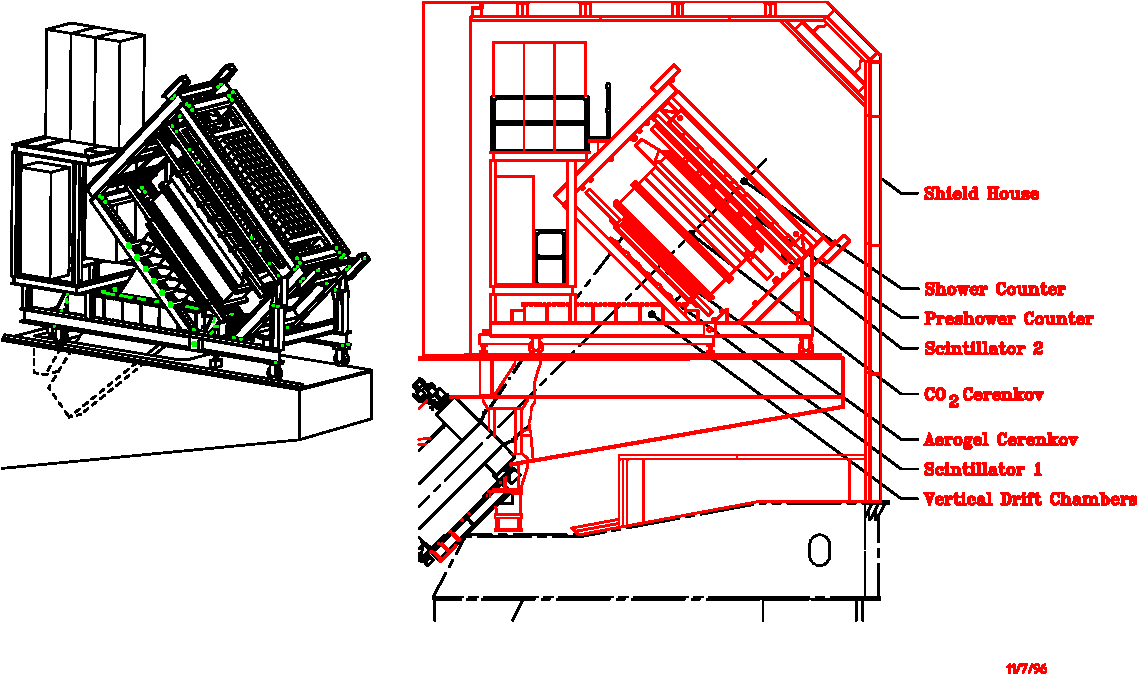
\includegraphics[angle=0,width=\textwidth,clip]{figure0103_r}
{\linespread{1.}
\caption[Spectrometers: Electron Arm Detectors]{The electron spectrometer detector stack.}
\label{fig:hrs_electron_det}}
\end{center}
\end{figure}

\begin{figure}[tbp]
\begin{center}
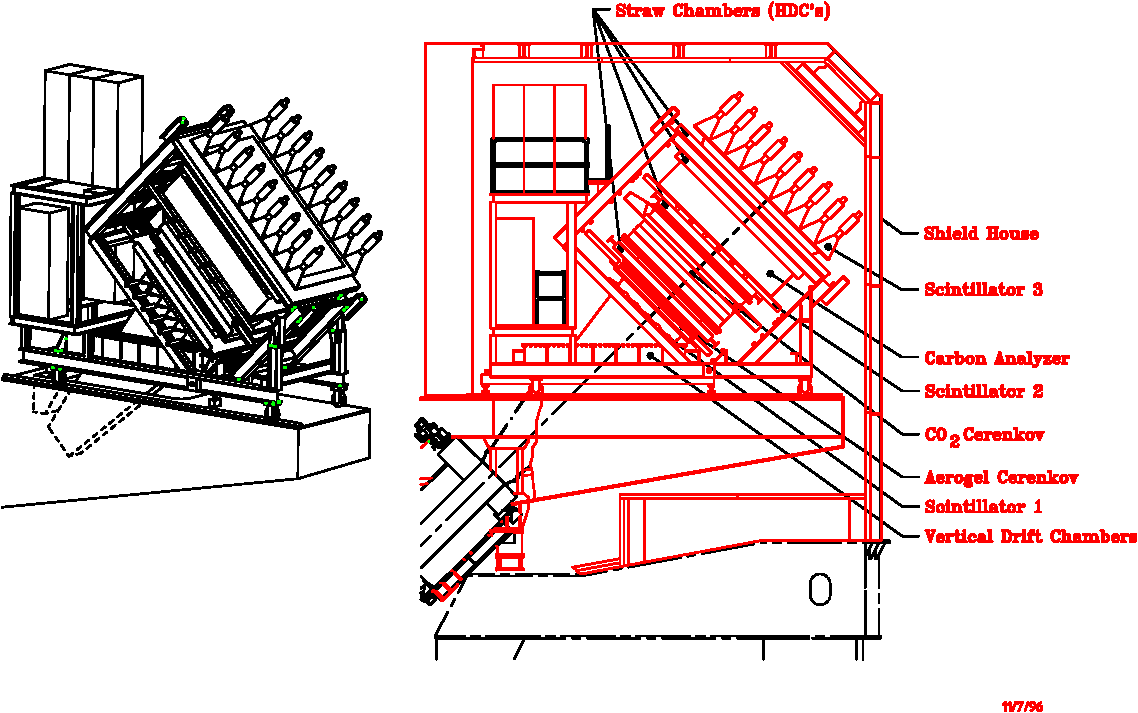
\includegraphics[angle=0,width=\textwidth,clip]{figure0104_r}
{\linespread{1.}
\caption[Spectrometers: Hadron Arm Detectors]{The hadron spectrometer detector stack.}
\label{fig:hrs_hadron_det}}
\end{center}
\end{figure}


The hadron detector is shown schematically in 
Figure~\ref{fig:hrs_hadron_det}.  It consists 
of two sets of (x,y) vertical drift wire chambers identical to those of the 
electron arm.  The remaining part of the detection system is used to 
define the level 1 trigger, as well as for particle identification and 
timing.  It consists of two minimally segmented planes of 
scintillation counters equipped with photomultipliers at both ends, and 
it includes \Cherenkov{} counters (gas CO$_2$ and Aerogel).

In addition, a proton polarimeter is installed in the back of the 
detector package to measure the polarization of the proton using a 
segmented carbon analyzer up to 60 cm in thickness to allow measurements 
over a wide range of proton energies.  A pair of front and a pair of 
rear straw tube wire chambers determine the incident and 
scattered angles, respectively.  The 
polarimeter detectors are dimensioned to accept a 20$^{\circ}$ cone of 
scattered protons.

Several support systems are necessary in addition to the basic 
components mentioned above.  They include gas supply systems for the 
wire chambers, high voltage supplies, readout electronics, a second 
level trigger, software for data analysis and testing, and a remotely 
controllable mechanical system.

For each spectrometer, all detectors are mounted on a 
single rigid support frame along with their associated electronics.  The trigger electronics are located on the support frame, next to the detectors.

To reduce the resolution degrading effects of multiple scattering, the 
entire interior of the spectrometer from the collimator box to the detector hut 
is a vacuum vessel.  The ends of this evacuated volume are capped by 
relatively thin vacuum windows.
}

\begin{safetyen}{0}{0}
\section{High Resolution Spectrometers}
\label{sec:hrs-safety}
\end{safetyen}

The principle concern with the spectrometers is that they are large, 
and have associated vacuum, hydraulic, cryogenic and magnet systems all of 
which can be potentially dangerous.

The bogies which move the massive 1200 ton spectrometers must be 
carefully operated.  Inspection of the floor and wheels to ensure there is no 
debris which the wheels could ride over is mandatory.  Similarly 
personnel need to be aware that the spectrometers are moving so that no one 
inadvertently gets trapped.

The vacuum systems associated with the spectrometers are essentially 
pressure vessels (see Chapter \ref{chap:vacuum} for more details).
Care should be exercised so as not to puncture the 
windows.

The magnets themselves are installed inside cryostats.  These vessels 
are exposed to high pressures and are therefore equipped with safety 
relief valves and burst discs.

The hydraulic system originally intended to operate the vertical positioning system (VPS) 
and the horizontal positioning system (HPS) has effectively been dismantled, after problems were encountered during the initial attempted operation of the system.

The cryogenic system operates at elevated pressure at 4K.  One must 
guard against cold burns and take the normal precautions with pressure 
vessels when operating this system.  Only authorized personnel are permitted to install 
and take out U tubes.

The magnets have a great deal of stored energy as they are large 
inductors. Always make sure people are clear of them and that
the dump resistor is attached to the magnet.

There are several major safety concerns with regards to the detectors, 
namely 1) flammable gas located in the VDC, 2) ODH hazard due to 
CO$_2$ in the \Cherenkov{} counter, 3) high voltage due to the photo 
multipliers on the various detectors and 4) a thin vacuum window 
separating the detector array from the vacuum system in the 
spectrometers.

\infolevltone{
\begin{safetyen}{5}{10}
For more information consult the full OSP manual~\cite{HallAosp}.
\end{safetyen}
} %infolev

\begin{safetyen}{10}{15}
\subsection{Authorized Personnel}
\end{safetyen}

In the event that problems arise during 
operation of the magnets, qualified personnel should be notified
(see Table \ref{tab:hrs:personnel}).  
This includes any prolonged or serious problem with the source of magnet 
cryogens (the ESR).  On weekends and after hours there will be a 
designated individual on call for magnet services.  Any member of the 
Hall A technical staff is qualified to deal with unusual magnet 
situations but in the event of serious problems the technician on
call should be contacted.

\begin{namestab}{tab:hrs:personnel}{HRS: authorized personnel}{%
      HRS: authorized personnel. ''W.B'' stands for the white board 
      in the counting house.}
   \TechonCall{\em Contact}
   \EdFolts{}
   \JackSegal{}
   \HeidiFansler{}
   \JessieButler{}
   \AndrewLumanog{}
   \JasonGlorioso{}
   \MahlonLong{}
\end{namestab}

\infolevone{
\section{The Magnets of HRS}

Each HRS is composed of three superconducting quadrupole magnets, Q1, Q2, 
and Q3, and one superconducting dipole magnet.  The large quadrupoles were 
manufactured for JLab by SIEMENS, the small quadrupole by SACLAY, while 
the dipole was built for JLab by WANG NMR.  The quadrupole magnets are 
referred to as Q1, Q2, and Q3, where a particle first traverses Q1, then 
Q2 and the dipole magnet and finally traverses Q3.

The magnet system is followed by a large steel and concrete detector 
hut, in which all detector elements reside.  Most of the 
detector elements have been built by universities involved in the Hall A 
physics program.

The HRS magnet system is the cornerstone of the Hall A activities.  
Many of the experiments approved in Hall A center on physics at high 
resolution and other short-range phenomena, and rely on a spectrometer 
able to momentum analyze charged particles up to very high momenta.  The 
design value for the maximum momentum accessible to the HRS magnet 
system is 4 GeV/c.
}

\subsection{Magnets and Power Supplies}

\infolevone{
The HRS magnet's are all superconducting and hence their coils must be 
maintained at cryogenic temperatures during operations.  The LHe 
required by the magnets is supplied by the End Station Refrigerator, ESR.

All the HRS magnets cryogenic services are supplied through the overhead 
cryogenic lines.  The distribution network begins at the distribution 
box over the pivot.  This box is connected to the rest of the network 
via the flexible transfer lines over the pivot.  The network is adjacent 
to the upstairs catwalk of the HRS.

Cryogenic information about each magnet is available on the control 
screens in the counting house, one for each magnet.  Normally during run 
periods the control screens are sent upstairs to the Hall A counting 
house and information on all the HRS magnets is available on the HRS 
control screen located in the center of the main console.  The control 
of all magnets is described in a following Section.

The power supplies for the magnets are located on the gantry balcony 
adjacent to the magnets.  The supplies are all cooled with low conductivity water (LCW).
}

\begin{safetyen}{10}{15}

Under no 
circumstances should any panel of any magnet power supply be opened by someone 
other than authorized personnel.  There are also 
signs posted listing the dangers of high magnetic fields.
\end{safetyen}

\infolevone{
A control interface for the power supplies is available through the 
HRS control screen in the Hall A counting house.
}

\infolevone{
\subsection{Quadrupole Magnets}

The quadrupoles provide some of the 
focusing properties of the spectrometer and to a large extent 
its acceptance.  Operating limits imposed on the 
quads are as follows: 1850A for Q2 and Q3 and 3250A 
for Q1.

All three quadrupoles for the HRS spectrometer are warm iron 
superconducting magnets.  The soft iron around the superconducting coil 
enhances the field at the coil center and reduces stray fields.  The 
basic parameters for the first quadrupole, Q1, are an effective length of about 
0.9 $m$, useful aperture of 0.3 $m$ and a field gradient of 9.5 
T/m.  To achieve the lowest possible angle setting of the HRS 
spectrometer (with respect to the beam line) the incident electron beam passes through
a notch in the outer yoke of Q1 when the spectrometer is at
its smallest angle of 12.5$^\circ$ . The 
other two quadrupoles, Q2 and Q3, are essentially identical with an 
effective (magnetic) length of about 1.8 meter, a useful aperture of 
0.6 $m$ and a field gradient of 3.5 T/m.
}

\infolevthree{
The maximum operating currents (assuming a 4 GeV/c momentum particle) 
for the quadrupoles are about 3000 A, 1700 A, and 1600 A, for Q1, Q2, and 
Q3, respectively.  This will render pole field values 
of 1.2, 1.0, and 1.0 T, respectively.  The energy stored in the 
quadrupole fields is sufficient to cause an unrecoverable quench if all 
the energy stored is dumped into the magnets.  Therefore a quench 
protection circuit is incorporated.  However, a quench can only happen 
if the cryomagnets have a helium level below the coil 60\% during operation.

The operating current to the Q1 quadrupole coils is provided by Danfysik 
System 8000 power supplies, which can operate up to 3500 A current and 5 
V.  The power supplies will be cooled with a combined maximum 
water flow of 45 liters per minute.

In addition to the main quadrupole windings, all quadrupoles have 
multipole windings.  To further optimize focusing properties of the HRS 
magnet system, it was intended to operate including some of these multipole 
trim coils in order to reduce higher order aberrations.
The operating current for these multipole corrections would be 
small, only (the multipole corrections are typically less than 2\% of 
the main quadrupole field), of order 50 A. Since the sextupoles were inadvertently 
installed rotated 90 $^\circ$ from their correct
orientation, these trim coils are now considered useless 
and there are at present no plans to use them.

\subsection{Cryogenic Procedures}

The cryogenics control is handled by the JLab Cryogenics Group.  The cryo control coordinator 
can be reached at the CHL (x7405) or by calling the MCC.

\subsection{First Time Startup Check List.}  

See attached check lists for all quadrupole and dipole magnets
 (Tables~\ref{tab:dip_check}, \ref{tab:q1_check}, and \ref{tab:q23_check}).
} %infolev

\infolevone{
\subsection{Dipole Magnet}

The dipole, by virtue of its field index, provides both
dispersion and focusing.  The present operations envelope 
states that the supply for the left HRS dipole may not be
operated at a current above 1800 A (4.4 GeV/c). The supply for the right HRS
dipole may not be operated above 1200 A (3.2 GeV/c), due to complications
caused by an internal short. 

The dipole for the HRS spectrometer is a superconducting, cryostable 
magnet.  Its basic parameters are an effective length of about 6.6 $m$, a 
bend radius of 8.4 $m$, and a gap width of 25 $cm$.  It is configured to 
achieve a 45 degree bending angle for 4 GeV/c momentum particles at a 
central field excitation of 1.6 T.  For the HRS dipole to reach 1.6 T 
an operating current of about 1500 A is required.
} %infolev

\infolevthree{
The dipole has been designed to achieve cryostability up to a field of 2 
T, and this property has been extensively tested up to a field of 1.6 T. 
 The cryostable coils are equipped with an energy removal circuit to 
cover the possibility of an unrecoverable quench.  However, this can 
only happen if the helium level drops below the coil during operation.  
The current to the coils will be provided by a Dynapower Corporation power 
supply, which can operate up to 2000 A and 10 V.  This 
power supply is located on the gantry beside the dipole, and will be 
cooled with a maximum water flow of 35 liters per minute.
The total water flow needed to cool the 4 power 
supplies for the HRS magnet system (dipole and quadrupoles) amounts to 
80 liters per minute, with a supply pressure of cooling water for Hall A 
of 100 psi.
} %infolev

\infolevtwo{
\section{Operation of the HRS Magnets}

\subsection{Introduction}

This is an abbreviated operating manual for 
the HRS superconducting magnets specifically designed for Hall A 
experimenters.  It provides instructions for setting currents, invoking 
NMR field regulation and general system monitoring.  Curious readers are 
directed to the references for more in-depth operating instructions and 
other technical manuals. Copies of the following supporting
documents are available in the Hall A Control Room and through the Hall A webpage
(see Table~\ref{tab:hrs-mag-manuals}).

\begin{table}[htp]
\begin{center}
\begin{tabular}{|l|l|}
\hline
References & \\
\hline 
WANG NMR Dipole & User Manual \\
Dynapower & Instruction Manual \\
Appendix & NMR Tesla meter \\
Appendix & NMR Field Regulation \\
Siemens/Fug & Q2/Q3 Magnet Instrumentation and Power Supplies \\
Saclay/Danfysik & Q1 Power Supply Manual \\
TOSP & HRS Dipole \\
TOSP & HRS Quadrupole Q1 \\
TOSP & HRS Quadrupole Q2, Q3 \\
HRS & SC Dipole Magnet Safety Review Vol. 2 \\
HRS & SC Quad Safety Review Vol. 1 \\ \hline
\end{tabular}
\end{center}
\caption[HRS Magnets: extra manuals]{HRS Magnets: extra manuals available in 
     Hall A Control Room.}
\label{tab:hrs-mag-manuals}
\end{table}

\subsection{Simple HRS Setting (Autopilot Mode)}
\label{sec:hrs-mag-set} 

 The magnets are controlled remotely using EPICS~\cite{EPICSwww} and
 EDM~\cite{EDMwww} GUI, provided that everything is working and power 
 supplies are turned on and ready to go.
 The appropriate interface runs
 on the computer \mycomp{hacsbc2} (see Section \ref{sec:contr-ha-menu}).
 On the ``Hall A General Tools'' control screen, in the upper left, there is 
 a rectangular box for each spectrometer (see Figure~\ref{fig:hrs_mag_cntrl}). 
\begin{figure}
\begin{center}
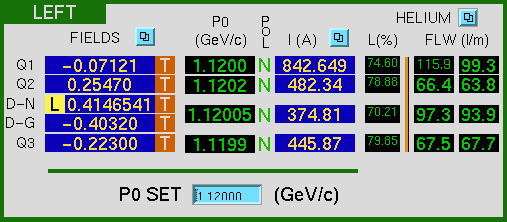
\includegraphics[angle=0,width=0.8\textwidth]{medm_halla_tools_1_cut1}
{\linespread{1.}
\caption[HRS: Magnets control]{A part of ``Hall A General Tools'' screen, 
        used for HRS (left) magnets control.}
\label{fig:hrs_mag_cntrl}}
\end{center}
\end{figure}

This box displays a brief summary of the status of the spectrometer
magnets and their cryogenic systems. The blue fields (with white
numbers) give readbacks of the magnetic fields and currents in each
magnet. The black fields also give readbacks, however in this case if
the text appears green those parameters are OK while if they are red
then that parameter is out of tolerance and may indicate a fault
condition. For example if the helium level goes below a certain point
the magnet will be automatically turned off.  In some cases it may be
desirable to monitor certain critical quantities on a strip chart
(e.g. magnet settings). A strip chart tool is available for this
purpose from the bottom of the ''EOS Menu'' button in the ''MyMenu'' window.

{\bf To set the spectrometers} for a given value of central momentum
(P0) type the desired P0 value into the light blue P0 SET box and hit
return. The magnets will be automatically 
set to the correct
values. All green numbers in the P0 column indicates that the desired
field or current settings have been reached. 

{\bf Caution:} Regarding the
dipoles, in general it's a bad idea to assume that at the first
instant that the P0 display turns green that the desired field has
been reached and you can start taking data. Stable field is in general
not achieved for from 15 to 30 minutes after reaching the nominal
desired field. This settling time depends on the magnet (the right dipole is
slower than the left dipole) and the magnitude of the field change (small
changes settle faster than big changes). Experimenters are advised to
observe both the field reading and current reading on the magnet in
question and verify that things are stable to their satisfaction
before proceeding.
 
\subsection{Powering Up Dipole Magnets:}

Use these instructions to recover from loss of a magnet due to a fault
(e.g. He level or lead flow fault). The order of actions matters. \\
(Contact Tech-On-Call if anything behaves funny or things don't
respond as expected. Sometimes after a trip an access to the Hall is
required to reset things).

\begin{list}{\arabic{enumi}.~}{\usecounter{enumi}\setlength{\itemsep}{-0.15cm}}
   \item Wait for Iout=0 (you can't and don't want to do anything while the magnet is in emergency fast dump mode.)
   \item While waiting, make a log entry re the fault. Give details such as time, coincident activities, and nature of the fault.
   \item Make sure the fault is cleared. (e.g. He level and flow rates returned to normal values and stable)
   \item In the HRS Right (Left) Dipole Systems' control panel:
   \begin{list}{}{\setlength{\itemsep}{-0.15cm}}
      \item[(a)] Press RESET (verify that all faults are cleared in the middle column)
      \item[(b)] Press ON (Display will indicate Power Supply ON and Magnet ENGAGED)
   \end{list}
\end{list}


Power supply and magnet are ready to go. From here you can return 
to "Autopilot Mode" (see Section \ref{sec:hrs-mag-set}).

\subsection{Starting Q1 Power Supply:}

 Do this when a fault causes the power supply to shut off.
 Wait for fault to clear (watch He levels). 
\begin{list}{\arabic{enumi}.~}{\usecounter{enumi}\setlength{\itemsep}{-0.15cm}}
   \item Push POWER OFF/RESET (check all faults cleared)
   \item Select desired polarity
   \item Push POWER ON
   \item Type in Setpoint (Amps) (light blue field) or re-enter P0 in Autopilot Mode.
\end{list}

\subsection{Starting Q2/3 Power Supply:}

 Do this when a fault causes the power supply to shut off.
 Wait for cause of fault to clear (watch He levels). 
 \begin{list}{\arabic{enumi}.~}{\usecounter{enumi}\setlength{\itemsep}{-0.15cm}}
   \item Push RESET 
   \item Select desired polarity
   \item Push ON
   \item Type in Current Set (light blue field) or re-enter P0 in Autopilot Mode.
\end{list}

} %infolev

\subsection{Rotation}
%
% Thanks to John LeRose for Rotation text. 07NOV2013
%
Moving an HRS
Since each HRS weighs in excess of 1,000 tons it is very important that all safety
precautions are carefully adhered to. The good news is they move very slowly (a few degrees/min
maximum), BUT 1,000 tons moving even very slowly is hard to stop. 

Hazards include:
\begin{itemize}
\item{Knocking items over.}
\item{The wheels crushing things (including fingers and toes) on the floor in the path of the 
spectrometer}
\item{Damaging the beamline or other equipment on the floor if one goes to too small 
or too large an angle, or if it just gets pushed around inadvertantly.}
\item{Tearing out of cables etc. physically attached to the superstructure}
\end{itemize}

Hazard mitigations:
\begin{itemize}
\item{Guards on either side of the wheels prevent items from getting under them.}
\item{Large pins in the floor to stop the spectrometer rotated beyond the needed angular range.}
\item{Blinking lights on the spectrometers indicating they are in motion or that motion
is possible (controls engaged etc.)}
\item{During a running experiment the run coordinator and work coordinator should know in advance 
of any moves.  Moves at any other time must be cleared with the Hall work coordinator 
before implementation.}
\item{Careful inspection of the intended path to make sure it is clear. This is part of
the pre-run checklist performed by the technical staff prior to closing the Hall and
a remote camera allows shift worker to inspect the area.}
%
%\item{Any motion that takes a spectrometer inside 14 degrees or outside x degrees
%(x being specified in the pre-run checklist and noted on the whiteboard during a run) 
%must be supervised by a trained Hall A technician.}
\end{itemize}

\infolevone{
Remote Procedure for a shift worker:
\begin{itemize}
\item{Make sure the move is part of the approved runplan (if in doubt, check with the 
run coordinator).}
\item{Check that the pre-run checklist has been completed and note and comply with any 
possible limitations to spectrometer motion (if there is a conflict inform the Run
Coordinator and do not initiate any move until the conflict is cleared).}
\item{Visually inspect the Hall using the closed circuit TV cameras to verify that there
are no obstructions.}
\item{If people are in the Hall wait until they leave (during a Controlled Access MCC keeps
track of people in the Hall). (Maybe we could soften this to "Inform EVERYONE in the Hall of
the move".)}
\item{Activate the spectrometer motion controls (see the Wiki and below) and 
move to the desired angle.}
\item{Deactivate the controls (brakes on, power off, etc.)}
\item{Update the spectrometer position information on the Hall A Controls screen}
\item{Make a halog entry indicating you've moved the spectrometer including from what angle 
to what new angle.}
\end{itemize}

Procedure for a non-run associated move in the Hall:
\begin{itemize}
\item{Inform the work coordinator of the planned move}
\item{Perform a careful visual inspection to verify that the path is clear}
\item{Check to make sure there are no temporary connections to the spectrometer (wires etc.)
that could be damaged during the move.}
\item{Inform everyone in the Hall of the move and check with them re 3.}
\item{Activate the spectrometer motion controls (see the Wiki and below) verify 
that the warning lights are on and move to the desired angle.}
\item{Deactivate the controls (brakes on, power off, etc.).}
\end{itemize}

The full proceedure for moving the spectrometer follows and can also be found on the Hall A wiki.

On hacsbc2, click the red "tool box" icon on the linux taskbar, as above. Choose 
bogies\_SetSpec so that you can determine the angle and vernier setting for the spectrometer.
Enter the spectrometer (L or R), and the angle, and you will get two options for the floor 
mark and the vernier. Generally choose the vernier closer to zero. Center the cameras on the 
desire vernier using the Move+/Move- buttons on the Hall A General Tools screen. The TV monitors 
for these cameras are on the middle shelf, in rack CH01A05.

Choose bogies\_Left (or bogies\_Right) in the tool box to bring up the bogies control screen. 
Click PSM enable and wait a few seconds for PSM OK to read YES. 
Click DM enable and wait a few seconds for DM OK to read YES.
Make sure the velocity is set to 0 and the direction is CW or CCW as desired. Click on Brake Release 
and wait for Brakes OK to read YES.

Click on ClampRelease, set the velocity to 700. Once you see the spectrometer start to move in the 
floor angle camera - you cannot see the spectrometer move in the Hall overview camera, as it only 
moves a few degrees per minute at maximum speed. For the left arm, to move to a larger angle, the 
direction should be CCW, while for the right arm CW moves the spectrometer to larger angle. The 
direction of the spectrometer is reversed by using a negative rpm. Watch the spectrometer motion 
on the cameras. When you are getting close to the desired angle, slow down to about 300 rpm. 
To stop, click on the Clamp Release button and the Brake button. Disable DM and PSM, and disconnect 
to close the GUI. Read off the floor angle mark and vernier, and input the values into the appropriate 
fields in the Alignment section of the Hall A General Tools GUI. 
}









\newpage
\section[Field Monitoring]{Field Monitoring
\footnote{
  $CVS~revision~ $Id: nmr-1999.tex,v 1.4 2003/12/17 03:59:48 gen Exp $ $ 
}
\footnote{Authors: J.LeRose \email{lerose@jlab.org}}
}

The field-monitoring controls are available using the main 
HRS screen%
\infolevtwo{ (see Figure~\ref{fig:hrs_mag_cntrl})%
}. % infolev
The dipoles' field is measured using NMR Teslameters and
field probes.

\infolevone{ 
 
\subsection{ Dipole Field Monitoring Electron Arm}

\noindent {\bf Basic Setup}

Each spectrometer dipole magnet is equipped with a Metrolab PT 4025 
NMR Teslameter, several field probes, and multiplexers (to allow switching 
between the probes).  Details of the operation and theory of operation 
for the Teslameter can be found in its user manual, 
a copy of which is available in the the counting house.
The basic layout is shown in Figure~\ref{fig:nmrbasic}


\begin{figure}
\begin{center}
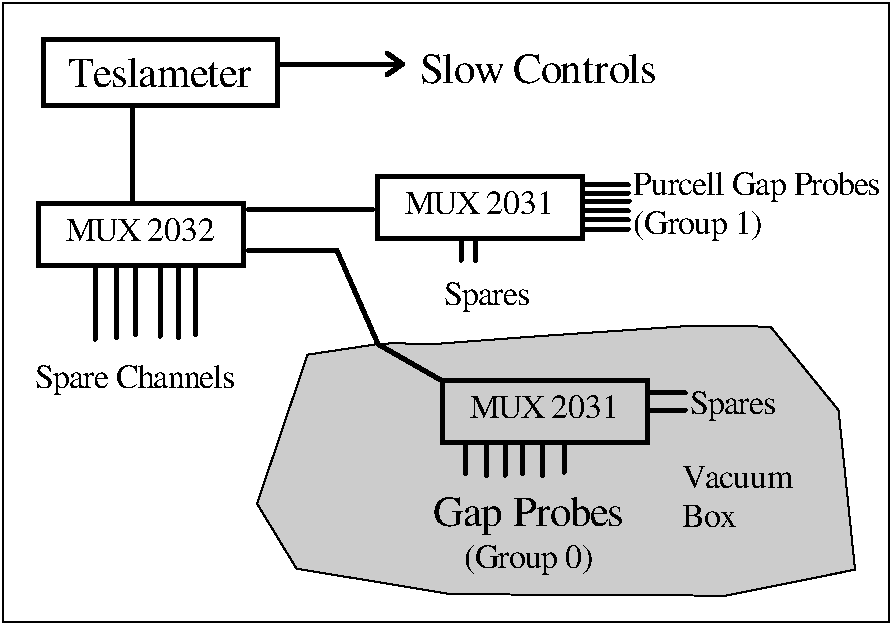
\includegraphics[angle=0,width=15cm,clip]{lerose_fig1}
{\linespread{1.}
\caption[Spectrometers: NMR System Layout]{Basic layout of NMR system}
\label{fig:nmrbasic}}
\end{center}
\end{figure}


 The "Gap Probes" (Group 0 in the controls) are located in two groups 
of three; one group on the low field side of the gap and the other on the high 
field side of the gap.  The groups of three are made up of one each of 
the manufacturer's type 3, 4 \& 5 probes, designed to cover different 
field ranges (see Table \ref{nmr_range}).  The six ``Purcell Gap Probes'' (Group 1 in 
the controls) are located in the Purcell gap of the magnet 
and consists of two each of the above types. {\em Note: Since
the fall of 1998 the multiplexer-multiplexer in both arms,
MUX 2032, has been removed and hence the ``Purcell Gap Probes'' are currently
unavailable. There are no plans to re-install this multiplexer.}

 The "Gap Probes" are equipped with coils which provide a field 
gradient that cancels out the field gradient of the magnet in the vicinity of 
the probe.  These gradient compensating coils are part of a simple circuit 
that is completely independent of the Teslameter.  The basic circuit for 
the compensating coils is shown in Figure~\ref{fig:nmrcir}


\begin{figure}
\begin{center}
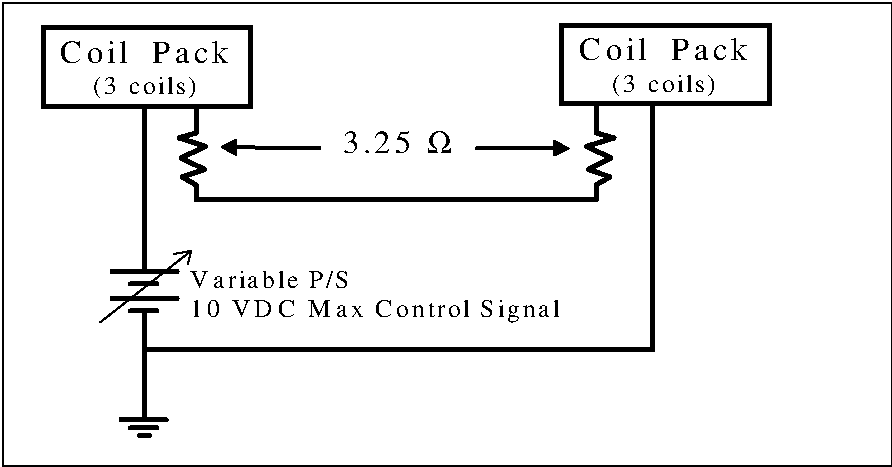
\includegraphics[angle=0,width=10cm,clip]{lerose_fig2}
{\linespread{1.}
\caption[Spectrometers: NMR Gradient Compensation]{Gradient Compensating Circuit.}
\label{fig:nmrcir}}
\end{center}
\end{figure}


%\snfig{figs/lerose_figcce.eps}{Control Voltage calibration for
%Electron Dipole }{nmrcomp4}{5in}

\begin{figure}
\begin{center}
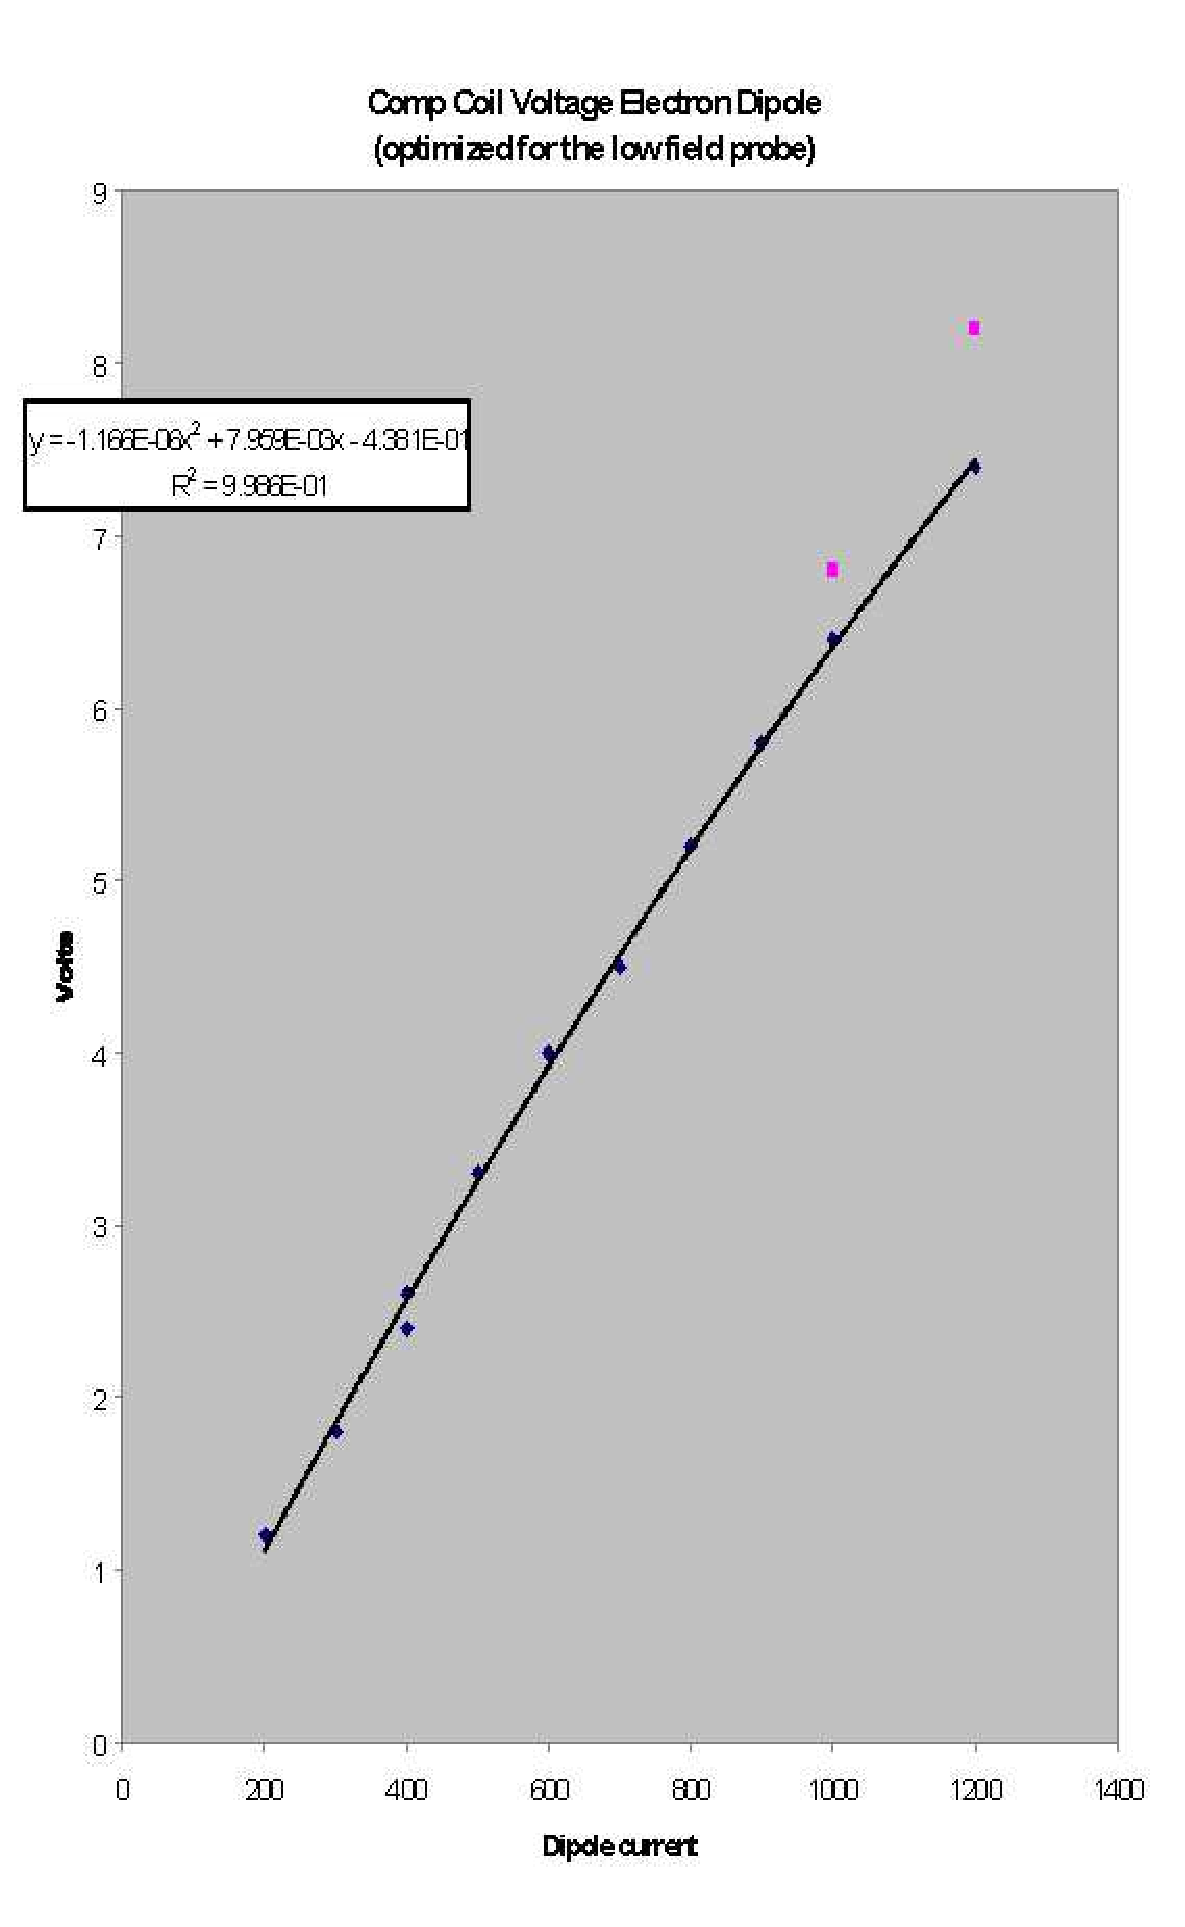
\includegraphics[angle=0,height=20cm,clip]{lerose_figcce}
{\linespread{1.}
\caption[Spectrometers: Control Voltage Calibration for Left Dipole]{Control Voltage calibration for the Left Dipole.}
\label{fig:nmrcomp4}}
\end{center}
\end{figure}

%\snfig{figs/lerose_figcch.eps}{Control Voltage calibration for
%Hadron Dipole }{nmrcomp5}{5in}
\begin{figure}
\begin{center}
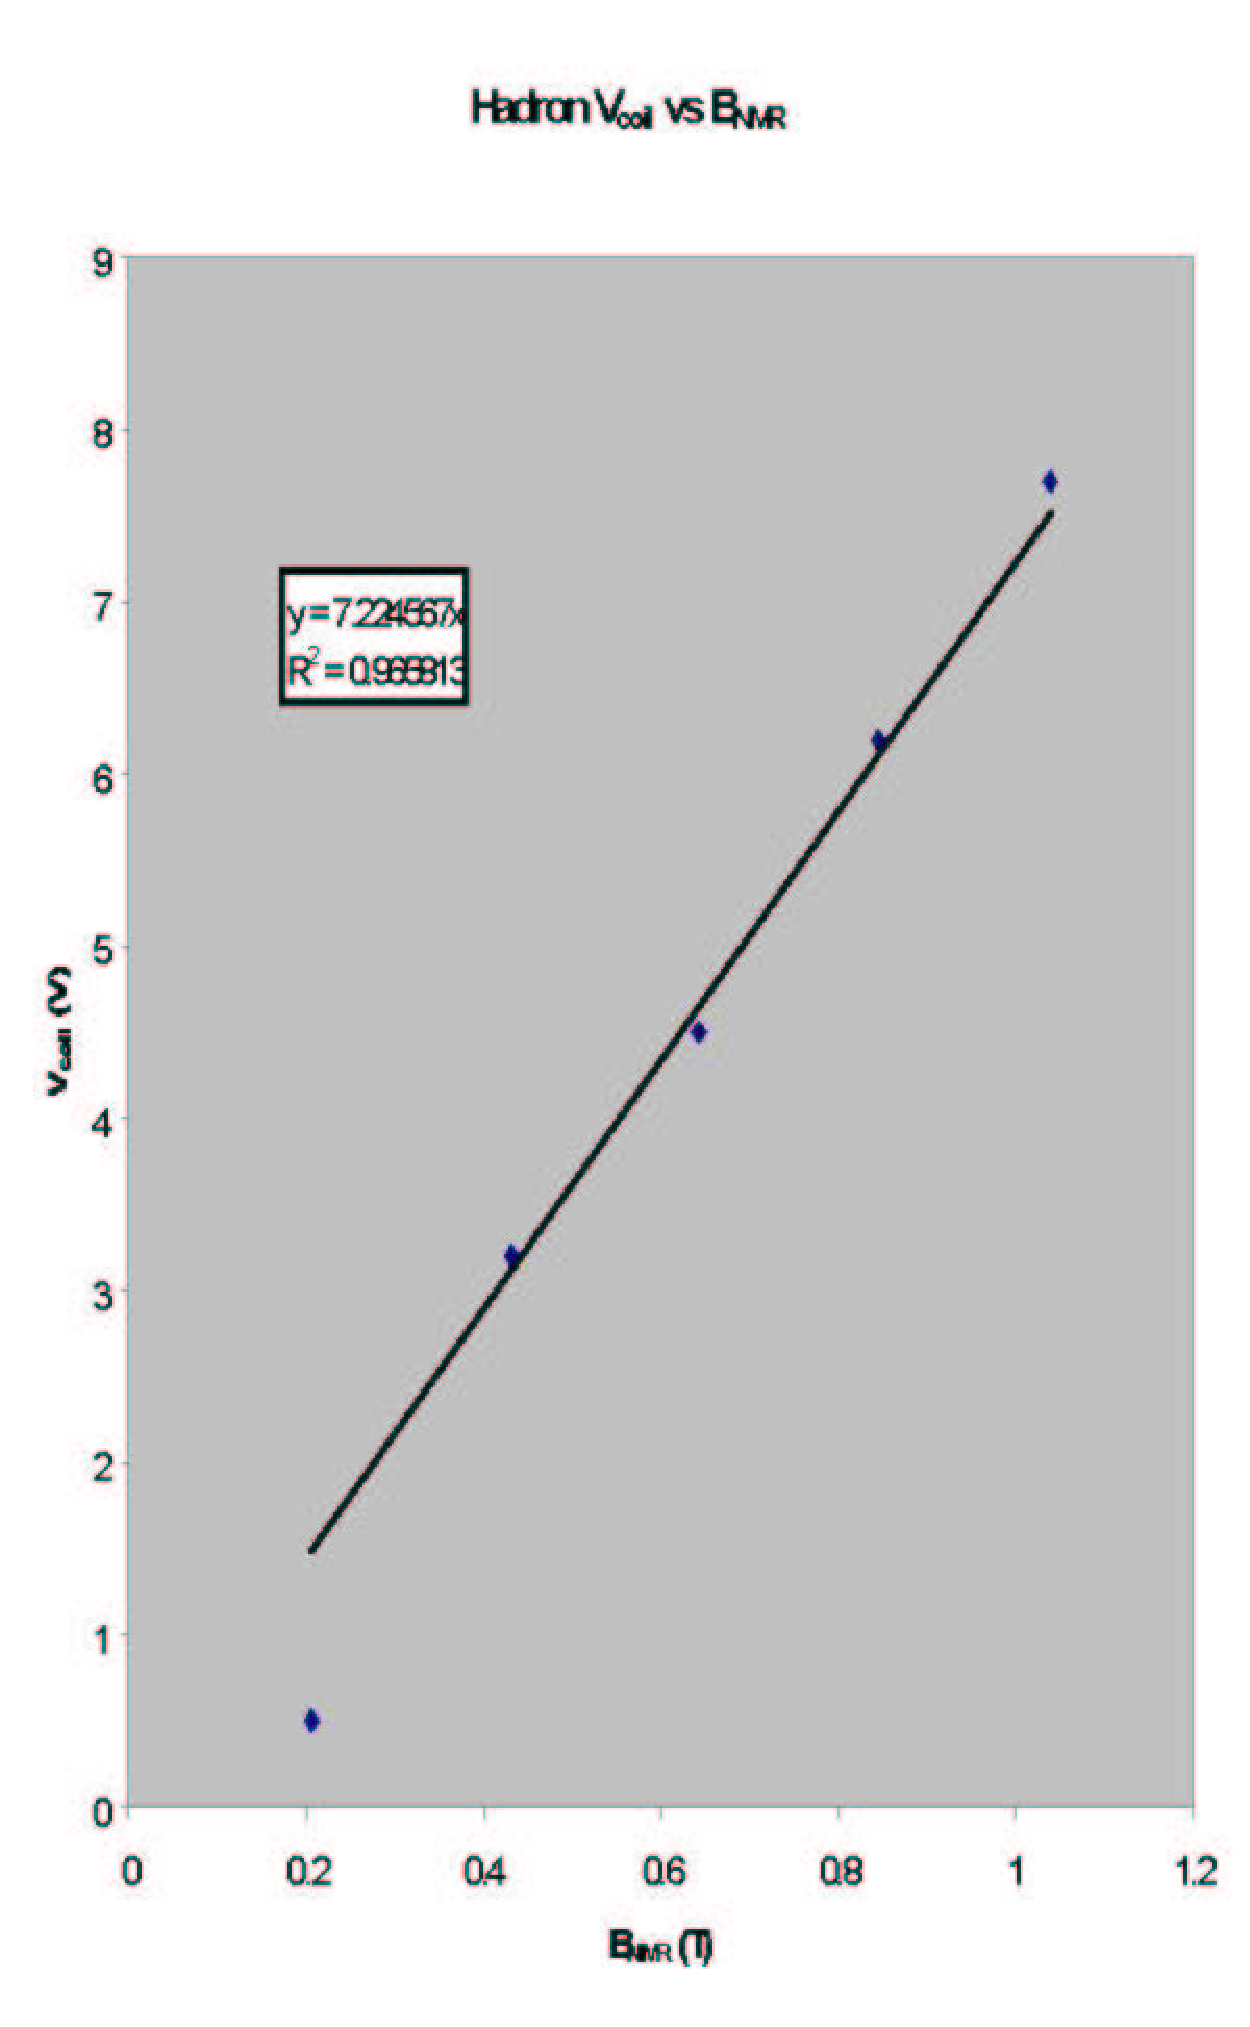
\includegraphics[angle=0,height=20cm,clip]{lerose_figcch}
{\linespread{1.}
\caption[Spectrometers: Control Voltage Calibration for Right Dipole] {Control Voltage calibration for the Right Dipole.}
\label{fig:nmrcomp5}}
\end{center}
\end{figure}

%\snfig{./figs/lerose_fig7.eps}{DAC Calibration for manual operation of NMR probes}{nmr_dac}{9in}
\begin{figure}
\begin{center}
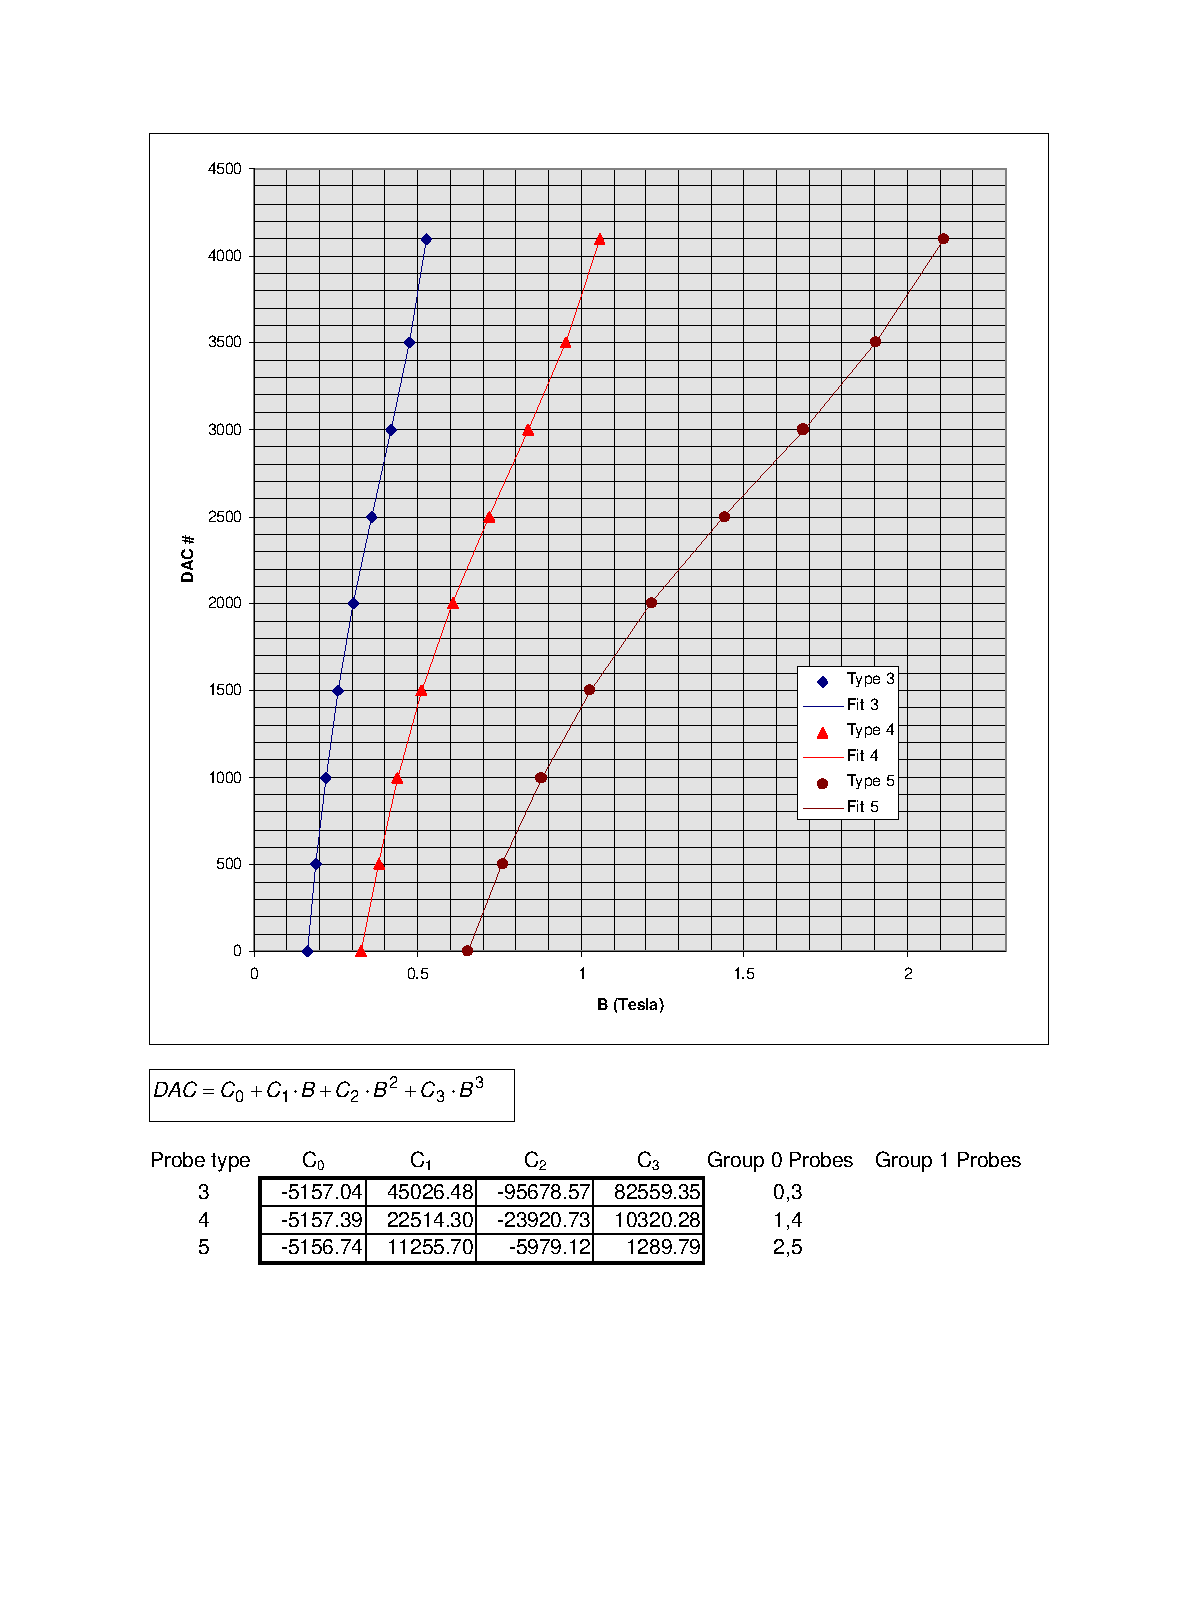
\includegraphics[angle=0,height=20cm,clip]{lerose_fig7}
{\linespread{1.}
\caption[Spectrometers: NMR Probe DAC Calibration]{DAC Calibration for manual operation of NMR probes.}
\label{fig:nmr_dac}}
\end{center}
\end{figure}

The following graphs (see Figures~\ref{fig:nmrcomp4} 
and ~\ref{fig:nmrcomp5}),can be used to determine optimum values for the 
compensating coil control voltage.  It should be noted that the setting 
of the compensating coil current is not very critical in most cases.  In 
general if you're within 10\% of the correct value everything should 
work fine.



\begin{table}
\begin{center}
\begin{tabular}{|cc|} \hline
Probe Type & Field Range (T) \\ \hline 
3 & 0.17 - 0.52 \\
4 & 0.35 - 1.05 \\
5 & 0.70 - 2.10 \\ \hline
\end{tabular}
\caption[Spectrometers: Dipole NMR Probe Field Ranges]{Dipole NMR probe field ranges}
\label{nmr_range}
\end{center}
\end{table}

} %infolev

\infolevtwo{
\subsection{NMR Operating Procedure}

When running in Autopilot mode (see: Simple Spectrometer Field Setting) the 
compensating coil voltage is set automatically and the probe appropriate for 
the field desired is selected. The gaussmeter is placed in SEARCH Mode and the 
dipole power supply software regulator is turned on. In this case the dipole current is 
adjusted to achieve the desired field. The user should just stand 
back and let it work. What follows are instructions for using
the NMR gaussmeter in situations where Autopilot doesn't work or
some special supplemental measurements are required. 

 In principle it is possible to make the field measurements using the 
SEARCH mode in the Teslameter.  In this mode you select a probe and the 
meter explores the whole field range of the probe until it finds and 
"locks" on the resonant signal indicating that it has a field 
measurement.  A ``lock" is indicated on the controls display by an ``L'' to 
the left of the field values.  This has the advantage of simplicity but in practice can 
be time consuming and doesn't always work.  The problem being, in 
situations where there is a lot of noise mixed in with the signal, the 
circuitry has problems distinguishing the signal from the noise and gets 
lost before it ever finds a lock.  The problem is exacerbated when the 
field being measured is at the high end of the probe's range.  In this 
case the search starts at the low end and keeps getting hung up on the 
noise and never gets to the field range of interest.  The solution to 
this problem is to tell the device approximately what field it's looking 
for and use the AUTO mode to find the lock.  In the procedure below that 
is what we will be doing.

In any case, for ``gap probes" (group 0) you must energize and adjust 
the gradient compensating coils for the field ranges to be measured before 
trying to make a measurement.

For studies involving 
10\% changes in the field settings the compensating coil current can be 
set once and left alone.


\noindent\underline{\bf Recommended Procedure:}(turn the {\bf SOFTWARE REGULATOR OFF} for all 
non-autopilot field measurements)\\
For group 0 probes set compensating coils appropriately (see figures).\\
Put the meter in MANUAL mode with SEARCH OFF \\
Select a probe \underline{\bf and} polarity (\underline{\bf Group 0:  
Probes 0, 1, 2 negative; Probes 3, 4, 5 positive}) \\
Type in the appropriate DAC number for the field range being measured (see below) \\
Select AUTO and wait for a lock (indicating a valid field reading) \\
Verify that you have a good lock by checking the oscilloscope for a 
clear resonant signal. \\
If you have problems see the table listing problems and possible 
solutions.

\noindent\underline{\bf Selecting DAC Number}

In selecting the DAC number to use for the field of interest use 
either the graph in Figure~\ref{fig:nmr_dac} or the polynomial at the bottom of the same figure.

\pagebreak
\noindent{\bf Problems and Solutions}\\
\begin{table}[htb]
\begin{tabular}{|p{0.4\textwidth}|p{0.55\textwidth}|}\hline
Symptom & Diagnosis and Cure \\ \hline\hline
Weird numbers on displays, controls for all magnets fouled up 
& Need to reboot.  See instructions below. \\ \hline
NMR Teslameter does not respond to commands and display shows all zeros. 
& Meter's communications are somehow hung up. Push {\bf RESET}. \\ \hline
%Will not lock & Very high noise level makes resonance hard to find. \\
%Still 
Will not lock 
& Very high noise level makes resonance hard to find. Search for the resonance manually by 
  adjusting the DAC in manual mode until you see the resonant signal.  (It helps if you know 
  what field you expect so you'll know where to look). \\ \hline
You find resonance manually but still can't get a lock 
& Check probe polarity. Try decreasing and increasing DAC number by 1. Optimize signal 
  by adjusting compensating coils. \\ \hline
Can't find resonance manually 
& Try a different probe.  Use readings from other probes to tell you where to look for 
 the resonance with the probe that's giving you trouble.  Make sure
 compensating coils are energized properly.  Make sure magnet is on. \\ \hline\hline
\end{tabular}
\caption[NMR: Problems and solutions]{NMR: Problems and solutions}
\label{tab:nmr-problems-solutions}
\end{table}

\begin{table}[ht]
\begin{center}
\begin{tabular}{|p{0.3\textwidth}|p{0.3\textwidth}|p{0.3\textwidth}|}\hline
Problems & Explanation & Action \\ \hline
NMR not locked but current is changing in the right direction 
& Normal operation for large field changes  
& Wait. (see above) \\ \hline
NMR locked but current going in the wrong direction.
& Normal operation. 
& Wait. \\ \hline
NMR locked but field not correct and current not changing 
& Field regulation is disabled or software is confused.
& Check that field regulation is enabled. Enter desired field value or one
  very near the desired value again. \\ \hline
NMR field display freezes. (Usually but not always shows  -\#.0000000)
& NMR Gaussmeter is not communicating with software.
& Push {\bf RESET}. \\ \hline
\end{tabular}
\end{center}
\caption[NMR troubleshhoting]{NMR troubleshooting
}
\label{tab:hrs_nmr_2}
\end{table}

} %infolev

\begin{safetyen}{10}{15}
\subsection{Authorized Personnel}
\end{safetyen}

The individuals shown in Table \ref{tab:nmr:personnel} are responsible for NMR operation problems.

\begin{namestab}{tab:nmr:personnel}{NMR: authorized personnel}{%
      NMR: authorized personnel.}
  \JavierGomez{\em Contact}
  \JohnLeRose{}
\end{namestab}



\newpage
\section[Collimators and Sieve Slits]{Collimators and Sieve Slits
\footnote{
  $CVS~revision~ $Id: slit.tex,v 1.5 2003/12/13 06:23:38 gen Exp $ $ 
}
\footnote{Authors: J.LeRose \email{lerose@jlab.org}}
}

Both spectrometers have front-end devices for calibrating the optical
properties of the spectrometers. These are known as the collimator boxes.
These boxes are positioned between the scattering chamber and the 
first quadrupoles (Q1). Each box is carefully aligned and rigidly attached
to the  entrance flange of the Q1 of the respective spectrometer.  The boxes are
part of the vacuum system of the spectrometer.
In the septum configuration sieve slits and collimators are installed and removed manually.

Inside each box a ladder is mounted which is guided by a linear bearing
and moved up and down by a ball screw. On this ladder 3 positions are 
available to insert collimators. Below this ladder
a special valve is mounted that can isolate the vacuum in the spectrometer
from the target system. This valve should be activated when it is moved
in front of the holes connecting the box with spectrometer and target chamber.
\infolevone{
A schematic view of the collimator box is shown in Fig.~\ref{fig:coll}.

\begin{figure}
\begin{center}
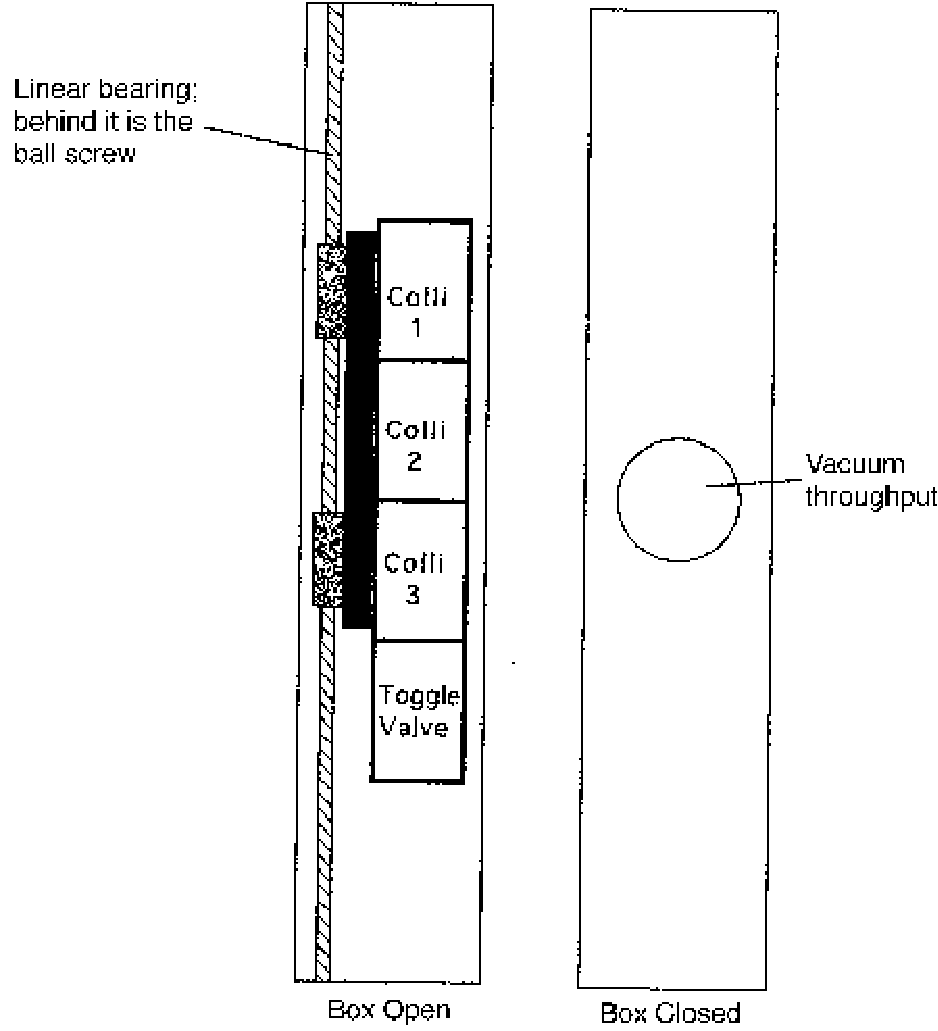
\includegraphics[angle=0,width=13cm,clip]{collimator_clip}
{\linespread{1.}
\caption[Spectrometers: Collimator Box Schematic]{Schematic layout of the collimator box.}
\label{fig:coll}}
\end{center}
\end{figure}
} %infolev

Vacuum requirement is $10^{-6}$ Torr. The material for the box is 
aluminum. It is possible to open one side of the box so that
collimators can be exchanged. The
reproducibility of collimator positions after moving
the ladder and/or after replacing a collimator is
better than 0.1 mm in horizontal and vertical direction.
The dimensions of the box are
roughly height=175 cm , width=35 cm and depth=15 cm.
The tolerance in the dimension
of the 7 msr collimator hole is $\pm0.5$ mm in each direction. 
The tolerance in the position
of each of the sieve-slit holes is $\pm0.1$ mm in each direction.

\infolevone{
\begin{figure}
\begin{center}
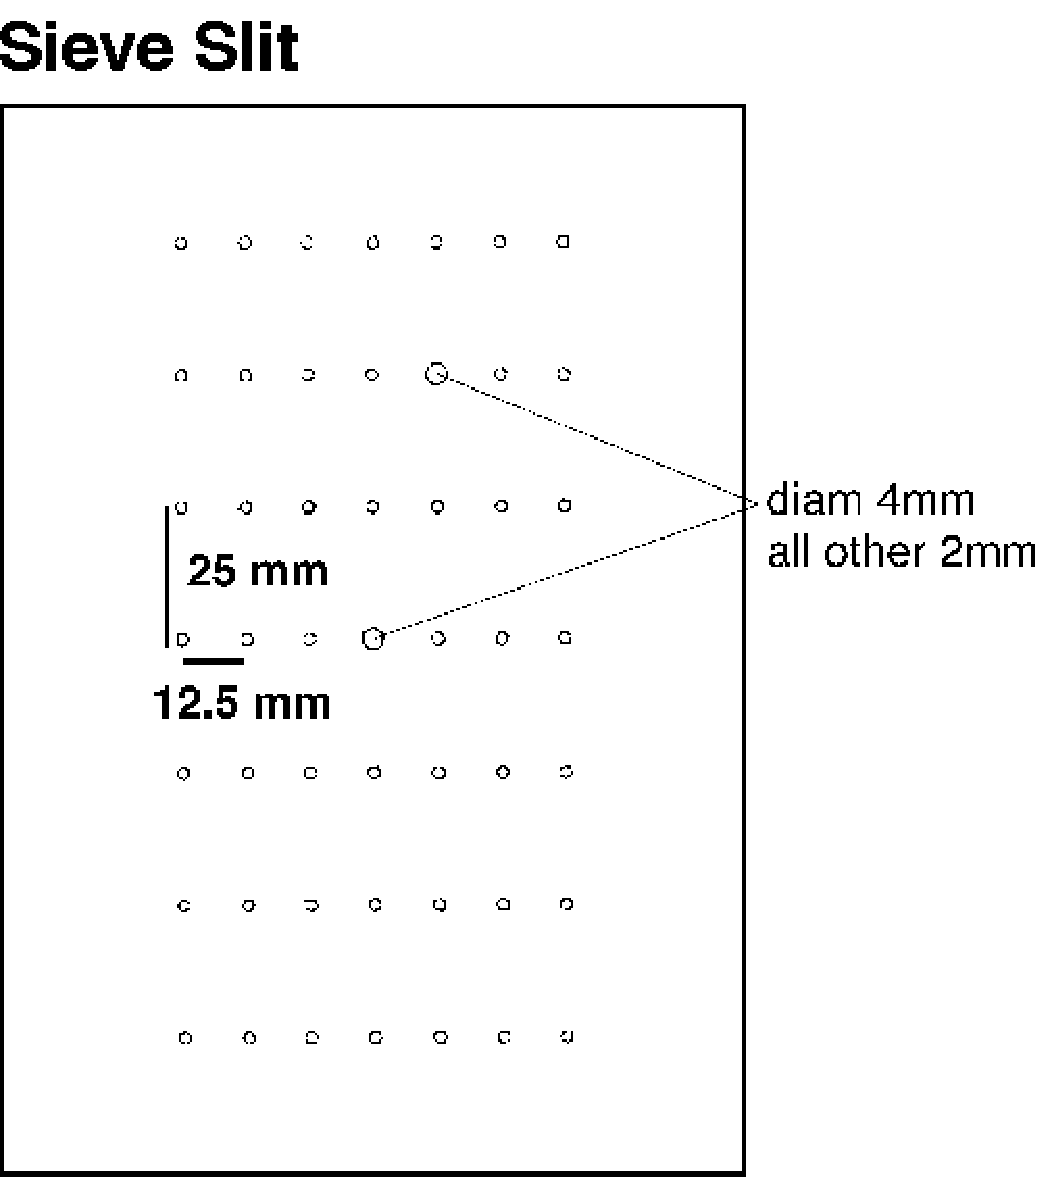
\includegraphics[angle=0,width=13cm,clip]{sieveslit}
{\linespread{1.}
\caption[Spectrometers: Sieve Slit]{Sieve slit collimator for optics calibration.}
\label{fig:sieve}}
\end{center}
\end{figure}
} %infolev
A typical sieve slit collimator 
\infolevone{(shown in Fig.~\ref{fig:sieve})
} %infolev 
consists of a plate of roughly 14 cm x 20 cm containing 49 holes
positioned in a regular 7x7 pattern. This slit is made out of 5
mm thick tungsten.
The holes have a diameter of 2 mm except for the central one and one positioned
off-diagonal which have a diameter of 4 mm. The horizontal distance between the
holes is 12.5 mm while the vertical distance is 25.0 mm.
%
%To get the latest information on the dimensions and locations of the collimators see 
%the Hall A homepage on the web%
%\htmladdnormallinkfoot{}{\url{
%http://hallaweb.jlab.org/
%}}.

To get the latest information on the dimensions and locations of the collimators see 
the Hall A homepage on the web%
\htmladdnormallinkfoot{}{\url{
http://hallaweb.jlab.org/
}}.

\begin{safetyen}{10}{15}
\subsection{Safety Assessment}

The collimator boxes form part of the vacuum system for each spectrometer. All hazards
identified in section spectrometer vacuum section applies to the collimator box as well.

In addition, safe access to the top of
the collimator boxes is needed  during manual operation of the box as outlined below.
Due to the proximity of the collimator boxes to the scattering chamber, and Q1 quadrupoles,
all necessary safety precautions with regards to vacuum windows, electrical power cables, 
cryogenic transfer lines, and high magnetic field should be taken. The same precautions also apply 
to the collimators and sieves in the septum configuration. In that case the sieve and collomators
can be considered part of the beamline. A survey and
appropriate RADCON designated proceedures must be followed when dealing with septum sieves 
and collimators.
\end{safetyen}

\infolevtwo{
\subsection{Operating Procedure}
Slit position is changed remotely from the standard Hall A control screen.
In the case of a spectrometer configuration involving the septum magnets collimators and sieves are
changed manually in the Hall.
} %infolev

\subsection{Authorized  Personnel} 

\begin{itemize} 
\item[~]E. Folts - x7857 (mechanical and vacuum systems).
\item[~]J. Gomez - x7498 (computer controls and electrical systems).
\end{itemize} 

% ===========  CVS info
% $Header: /group/halla/analysis/cvs/tex/osp/src/hrs/slit.tex,v 1.5 2003/12/13 06:23:38 gen Exp $
% $Id: slit.tex,v 1.5 2003/12/13 06:23:38 gen Exp $
% $Author: gen $
% $Date: 2003/12/13 06:23:38 $
% $Name:  $
% $Locker:  $
% $Log: slit.tex,v $
% Revision 1.5  2003/12/13 06:23:38  gen
% Septum added. Name tables. Polishing
%
% Revision 1.4  2003/12/05 06:49:07  gen
% infolevels added, polishing
%
% Revision 1.3  2003/06/06 16:13:37  gen
% Revision printout changed
%
% Revision 1.2  2003/06/05 23:30:00  gen
% Revision ID is printed in TeX
%
% Revision 1.1.1.1  2003/06/05 17:28:31  gen
% Imported from /home/gen/tex/OSP
%
%  Revision parameters to appear on the output

\newpage
\infolevtwo{
\section[Spectrometer Alignment]{Spectrometer Alignment
\footnote{
  $CVS~revision~ $Id: AlignmentOps.tex,v 1.8 2003/12/17 03:59:48 gen Exp $ $ 
}
\footnote{Authors: J.Gomez \email{gomez@jlab.org}}
}

At present, the systems implemented to determine the alignment of each spectrometer
(roll, vertical angle/pointing and horizontal angle/pointing) without the help of the
Accelerator Division Survey group are limited to roll, vertical angle and horizontal angle.
All alignment information is displayed in the ``ALIGNMENT'' mosaic of the ``Hall A
General Tools'' EDM screen%
\infolevtwo{ (see Fig.~\ref{fig:medm-hlamain-tools})}
(``EOS Menu'' $-->$ ``EDM (HLA Main)'' $-->$ ``Hall A Main Menu'' $-->$ ``Tools'').

A bi-axial inclinometer is used to determine the roll and vertical angle (also known as pitch)
of each spectrometer. These inclinometers are attached to the back of the dipoles at the power
supply platform level. The raw inclinometer measurements, in Volts,
are displayed as ``Tilt X'' and ``Tilt Y''. The inclinometer temperature is also given
(`` Tilt T''), in degree Celsius. From these values, the ``ROLL'' and ``PITCH'' values are
calculated.
Agreement between the inclinometer readings and survey measurements
are better than $\pm$ 0.1 mrad over all presently available history.

The horizontal spectrometer angle is determined from floor marks set in
place by the survey group. Floor marks have been placed every 0.5 $^\circ$ covering the useful range of
both spectrometers.
There are two concentric rings of floor marks in the hall. We will concentrate in the
inner ring which covers the angular range of both spectrometers. The outer ring is
similar.
The inner-ring floor marks are located at a distance of $\sim$10 $m$ from the target center.
A ruler attached to each spectrometer dipole runs over the floor marks and it acts as a vernier to interpolate
between marks. The location of a given floor mark on the ruler can be viewed from the Hall A Counting
House through a TV camera (labeled ``Front Camera'') .
The camera is able to move along the length of the ruler so that any
parallax effect can be eliminated. The camera motion is controlled from the ``Tools'' screen
through two push buttons (``FRONT CAMERA'' - ``MOVE +'' and ``MOVE --'').
Two fields in the ``ALIGNMENT'' mosaic
(``Flr Mrk'' and ``Vernier'') allow to input
the values read from the TV monitor. The effective spectrometer angle is then calculated and displayed
as ``Angle''. The application ``HRS Floor Marks'' calculates the floor mark and vernier value
to which the spectrometer should be set
to obtain a given angle. Spectrometer horizontal angle surveys and floor mark determinations
agree to $\pm$ 0.2 mrad.

\newpage
\begin{safetyen}{10}{15}
\subsection{Authorized  Personnel} 
\end{safetyen}
The authorized personnel is shown in table \ref{tab:align:personnel}.
\begin{namestab}{tab:align:personnel}{HRS alignment: authorized personnel}{%
      HRS alignment: authorized personnel.}
  \JessieButler{\em Contact}
\end{namestab}

} %infolev


% ===========  CVS info
% $Header: /group/halla/analysis/cvs/tex/osp/src/hrs/all.tex,v 1.3 2003/06/06 15:44:08 gen Exp $
% $Id: all.tex,v 1.3 2003/06/06 15:44:08 gen Exp $
% $Author: gen $
% $Date: 2003/06/06 15:44:08 $
% $Name:  $
% $Locker:  $
% $Log: all.tex,v $
% Revision 1.3  2003/06/06 15:44:08  gen
% Revision printout changed
%
% Revision 1.2  2003/06/05 23:30:00  gen
% Revision ID is printed in TeX
%
% Revision 1.1.1.1  2003/06/05 17:28:31  gen
% Imported from /home/gen/tex/OSP
%
%  Revision parameters to appear on the output

\chapter{High Resolution Spectrometers (HRS)}
\graphicspath{{hrs/figs/}}
\renewcommand{\dirfig}[0]{hrs/figs}
\renewcommand{\dircur}[0]{hrs}

\infolevone{
\chapter[High Resolution Spectrometers (HRS)]{High Resolution Spectrometers (HRS)
}
\footnote{Authors: J.LeRose \email{lerose@jlab.org}}
}
\label{chap:hrs}

\infolevone{
\section{Overview}
   
The Hall A spectrometers and associated instrumentation are designed to 
perform high resolution and high accuracy experiments.  The goal is to 
achieve a missing mass resolution of $\sim$ 200-500 keV to clearly 
identify the nuclear final state.  An absolute accuracy of $\sim$ 1\% is 
also required by the physics program planned in the Hall, which implies 
$\sim$ 10$^{-4}$ accuracy in the determination of particle momenta and 
$\sim$ 0.1 mr in the knowledge of the scattering angle.

The instruments needed are a high resolution electron spectrometer 
(HRES) and a high resolution hadron spectrometer (HRHS), both with a 
large angular and momentum acceptance.

\begin{figure}[tbp]
\begin{center}
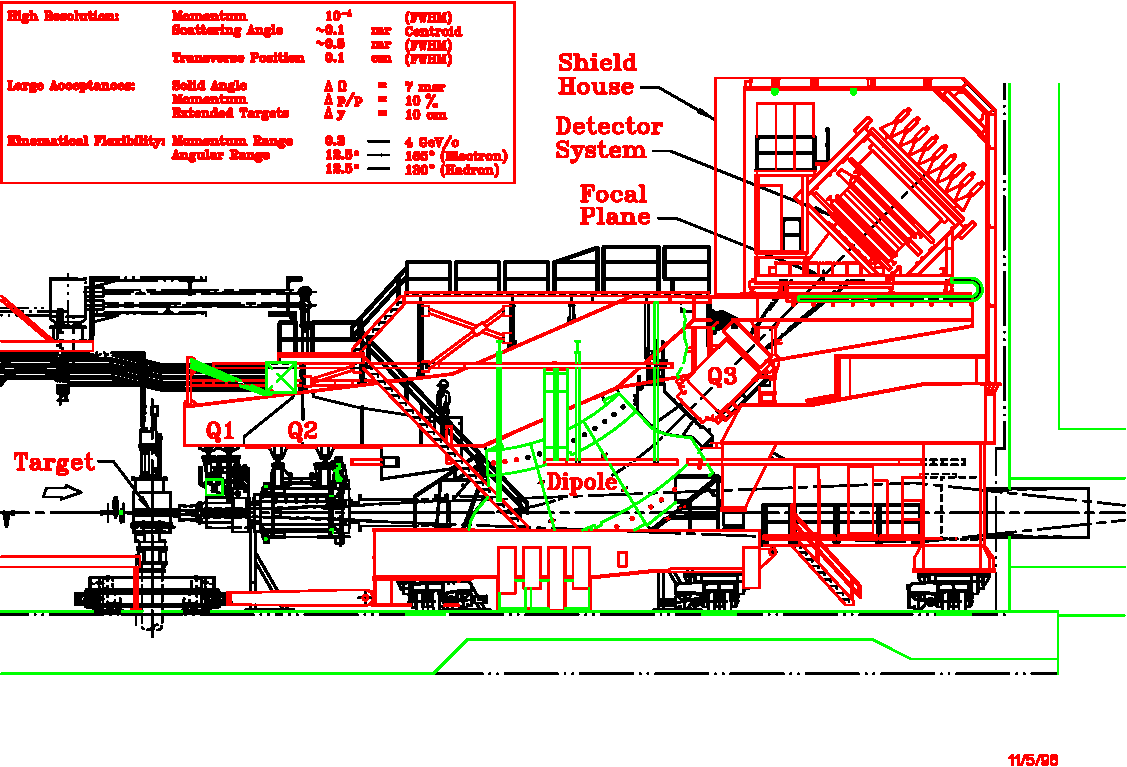
\includegraphics[angle=0,width=0.9\textwidth,clip]{figure0101_r}
\caption[Spectrometers: Elevation View of Hall~A HRS]{A side view of the Hall~A
HRS spectrometer.}  
\label{fig:hrs_ev}
\end{center}
\end{figure}
 
\begin{figure}[tbp]
\begin{center}
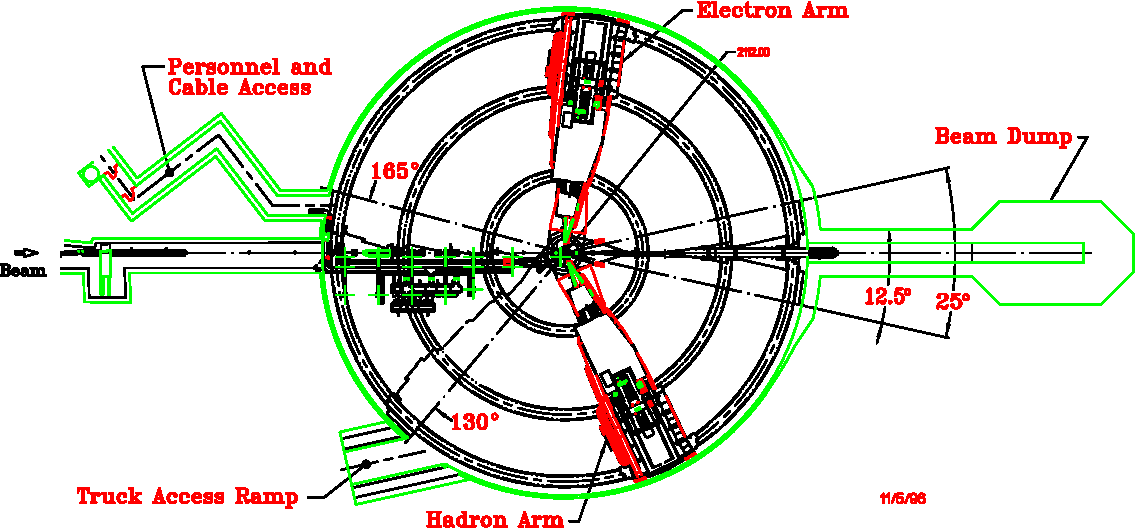
\includegraphics[angle=0,width=0.9\textwidth,clip]{figure0102_r}
\caption[Spectrometers: Plan View of Hall~A]{A bird's eye view of the Hall~A
end-station at TJNAF.}  
\label{fig:hrs_pv}
\end{center}
\end{figure}


A layout of the 4 GeV/c High Resolution Electron Spectrometer is shown 
on Figures~\ref{fig:hrs_pv} and \ref{fig:hrs_ev}.
Its main design characteristics are 
given in the attached table.  The spectrometer has a vertical bending 
plane and 45$^{\circ}$ bending angle.  The QQDQ design includes four 
independent superconducting magnets, three current-dominated 
cos2$\theta $ quadrupoles and one iron-dominated dipole with 
superconducting racetrack coils.  The second and third quadrupoles of 
each spectrometer have sufficiently similar field requirements that they 
are of identical design and construction.  The overall optical length, 
from target to focal plane, is 23.4 m.  Optically, the HRHS 
is essentially identical to HRES. In fact the two spectrometers can be used 
interchangeably to detect either positively or negatively charged particles 
as needed by any particular experiment. They are now commonly refered to 
as ``The Left Arm'' and ``The Right Arms'' rather than ``Hadron'' and ``Electron'' 

The support structure includes all system elements which bear the weight 
of the various spectrometer components and preserve their spatial 
relationship as required for 45$^{\circ}$ vertical bending optics.

The alignment and positioning system includes all the elements which 
measure and adjust the spatial relationship.  The support structure 
consists of the fabricated steel components which support the magnets, 
detector, shield house and associated equipment.  It is composed of the 
box beam, which supports the outer elements in fixed relative position 
atop the dipole; the dipole support bracket, upon which the dipole rests on 
the jacks; the cradle, upon which the dipole rests through the vertical 
positioning system, VPS; and a portion of the shield house load through 
the inboard legs of the gantry; the gantry, which supports the shield 
house and the magnet power supplies; and the bogies, which support the 
cradle-gantry assembly and roll on the floor plates and provide the 
driving power to move the two spectrometer arms.

The detector package (described in detail in Chapter \ref{chap:hrs-det})
is supported on the box beam and is surrounded by 
the shield house.  It must perform two functions, tracking and particle 
identification, PID.  The most important capability of focusing 
spectrometers is measuring precisely the momenta and entrance 
orientations of the tracks.  Momentum resolution of 10$^{-4}$ is 
obtainable, consistent with the resolution of the incident beam.

The actual configuration of the detector package varies from experiment to
experiment. The description given here is only an example of what is possible.
}

\infolevone{
A particle traversing the detector stack 
(Figure~\ref{fig:hrs_electron_det}) encounters two sets of horizontally
mounted, vertical drift wire chambers (x,y) with two planes of 368
wires in each chamber. The track resolution is $\sim$ 100 $\mu$m.  
From the chamber information both 
positions and angles in the dispersive and transverse directions can be 
determined.  The information from these chambers is the principal input 
of the tracking algorithms.

The chambers are followed by a scintillator hodoscope plane designated S1. 
This plastic scintillator array provides the timing reference for 
the drift chambers, and is also used in trigger formation and in combination 
with a second hodoscope pair it can provide time of flight particle 
identification.  These scintillators can also be used to perform crude 
tracking.

The next element encountered by a particle is a gas threshold \Cherenkov{} 
detector.  This is used for particle identification.  This gas threshold \Cherenkov{} detector can be swapped 
against an Aerogel detector, with a similar function.

The second hodoscope plane, S2, is located directly behind the 
gas \Cherenkov{}.  Its function is essentially the same as that of S1.  
In the hadron spectrometer an option exists to have this hodoscope 
pair be preceded by a third chamber, to improve tracking.
 Each of the two spectrometers 
have gas and Aerogel \Cherenkov{} detectors which can be used
 when they are in electron detection mode.

The final elements in the detector stack on HRSE are 
the pre-shower and the total-absorber lead glass shower 
calorimeter.  This is used for energy determination and PID.

\begin{figure}[tbp]
\begin{center}
\includegraphics[angle=0,width=\textwidth,clip]{figure0103_r}
{\linespread{1.}
\caption[Spectrometers: Electron Arm Detectors]{The electron spectrometer detector stack.}
\label{fig:hrs_electron_det}}
\end{center}
\end{figure}

\begin{figure}[tbp]
\begin{center}
\includegraphics[angle=0,width=\textwidth,clip]{figure0104_r}
{\linespread{1.}
\caption[Spectrometers: Hadron Arm Detectors]{The hadron spectrometer detector stack.}
\label{fig:hrs_hadron_det}}
\end{center}
\end{figure}


The hadron detector is shown schematically in 
Figure~\ref{fig:hrs_hadron_det}.  It consists 
of two sets of (x,y) vertical drift wire chambers identical to those of the 
electron arm.  The remaining part of the detection system is used to 
define the level 1 trigger, as well as for particle identification and 
timing.  It consists of two minimally segmented planes of 
scintillation counters equipped with photomultipliers at both ends, and 
it includes \Cherenkov{} counters (gas CO$_2$ and Aerogel).

In addition, a proton polarimeter is installed in the back of the 
detector package to measure the polarization of the proton using a 
segmented carbon analyzer up to 60 cm in thickness to allow measurements 
over a wide range of proton energies.  A pair of front and a pair of 
rear straw tube wire chambers determine the incident and 
scattered angles, respectively.  The 
polarimeter detectors are dimensioned to accept a 20$^{\circ}$ cone of 
scattered protons.

Several support systems are necessary in addition to the basic 
components mentioned above.  They include gas supply systems for the 
wire chambers, high voltage supplies, readout electronics, a second 
level trigger, software for data analysis and testing, and a remotely 
controllable mechanical system.

For each spectrometer, all detectors are mounted on a 
single rigid support frame along with their associated electronics.  The trigger electronics are located on the support frame, next to the detectors.

To reduce the resolution degrading effects of multiple scattering, the 
entire interior of the spectrometer from the collimator box to the detector hut 
is a vacuum vessel.  The ends of this evacuated volume are capped by 
relatively thin vacuum windows.
}

\begin{safetyen}{0}{0}
\section{High Resolution Spectrometers}
\label{sec:hrs-safety}
\end{safetyen}

The principle concern with the spectrometers is that they are large, 
and have associated vacuum, hydraulic, cryogenic and magnet systems all of 
which can be potentially dangerous.

The bogies which move the massive 1200 ton spectrometers must be 
carefully operated.  Inspection of the floor and wheels to ensure there is no 
debris which the wheels could ride over is mandatory.  Similarly 
personnel need to be aware that the spectrometers are moving so that no one 
inadvertently gets trapped.

The vacuum systems associated with the spectrometers are essentially 
pressure vessels (see Chapter \ref{chap:vacuum} for more details).
Care should be exercised so as not to puncture the 
windows.

The magnets themselves are installed inside cryostats.  These vessels 
are exposed to high pressures and are therefore equipped with safety 
relief valves and burst discs.

The hydraulic system originally intended to operate the vertical positioning system (VPS) 
and the horizontal positioning system (HPS) has effectively been dismantled, after problems were encountered during the initial attempted operation of the system.

The cryogenic system operates at elevated pressure at 4K.  One must 
guard against cold burns and take the normal precautions with pressure 
vessels when operating this system.  Only authorized personnel are permitted to install 
and take out U tubes.

The magnets have a great deal of stored energy as they are large 
inductors. Always make sure people are clear of them and that
the dump resistor is attached to the magnet.

There are several major safety concerns with regards to the detectors, 
namely 1) flammable gas located in the VDC, 2) ODH hazard due to 
CO$_2$ in the \Cherenkov{} counter, 3) high voltage due to the photo 
multipliers on the various detectors and 4) a thin vacuum window 
separating the detector array from the vacuum system in the 
spectrometers.

\infolevltone{
\begin{safetyen}{5}{10}
For more information consult the full OSP manual~\cite{HallAosp}.
\end{safetyen}
} %infolev

\begin{safetyen}{10}{15}
\subsection{Authorized Personnel}
\end{safetyen}

In the event that problems arise during 
operation of the magnets, qualified personnel should be notified
(see Table \ref{tab:hrs:personnel}).  
This includes any prolonged or serious problem with the source of magnet 
cryogens (the ESR).  On weekends and after hours there will be a 
designated individual on call for magnet services.  Any member of the 
Hall A technical staff is qualified to deal with unusual magnet 
situations but in the event of serious problems the technician on
call should be contacted.

\begin{namestab}{tab:hrs:personnel}{HRS: authorized personnel}{%
      HRS: authorized personnel. ''W.B'' stands for the white board 
      in the counting house.}
   \TechonCall{\em Contact}
   \EdFolts{}
   \JackSegal{}
   \HeidiFansler{}
   \JessieButler{}
   \AndrewLumanog{}
   \JasonGlorioso{}
   \MahlonLong{}
\end{namestab}

\infolevone{
\section{The Magnets of HRS}

Each HRS is composed of three superconducting quadrupole magnets, Q1, Q2, 
and Q3, and one superconducting dipole magnet.  The large quadrupoles were 
manufactured for JLab by SIEMENS, the small quadrupole by SACLAY, while 
the dipole was built for JLab by WANG NMR.  The quadrupole magnets are 
referred to as Q1, Q2, and Q3, where a particle first traverses Q1, then 
Q2 and the dipole magnet and finally traverses Q3.

The magnet system is followed by a large steel and concrete detector 
hut, in which all detector elements reside.  Most of the 
detector elements have been built by universities involved in the Hall A 
physics program.

The HRS magnet system is the cornerstone of the Hall A activities.  
Many of the experiments approved in Hall A center on physics at high 
resolution and other short-range phenomena, and rely on a spectrometer 
able to momentum analyze charged particles up to very high momenta.  The 
design value for the maximum momentum accessible to the HRS magnet 
system is 4 GeV/c.
}

\subsection{Magnets and Power Supplies}

\infolevone{
The HRS magnet's are all superconducting and hence their coils must be 
maintained at cryogenic temperatures during operations.  The LHe 
required by the magnets is supplied by the End Station Refrigerator, ESR.

All the HRS magnets cryogenic services are supplied through the overhead 
cryogenic lines.  The distribution network begins at the distribution 
box over the pivot.  This box is connected to the rest of the network 
via the flexible transfer lines over the pivot.  The network is adjacent 
to the upstairs catwalk of the HRS.

Cryogenic information about each magnet is available on the control 
screens in the counting house, one for each magnet.  Normally during run 
periods the control screens are sent upstairs to the Hall A counting 
house and information on all the HRS magnets is available on the HRS 
control screen located in the center of the main console.  The control 
of all magnets is described in a following Section.

The power supplies for the magnets are located on the gantry balcony 
adjacent to the magnets.  The supplies are all cooled with low conductivity water (LCW).
}

\begin{safetyen}{10}{15}

Under no 
circumstances should any panel of any magnet power supply be opened by someone 
other than authorized personnel.  There are also 
signs posted listing the dangers of high magnetic fields.
\end{safetyen}

\infolevone{
A control interface for the power supplies is available through the 
HRS control screen in the Hall A counting house.
}

\infolevone{
\subsection{Quadrupole Magnets}

The quadrupoles provide some of the 
focusing properties of the spectrometer and to a large extent 
its acceptance.  Operating limits imposed on the 
quads are as follows: 1850A for Q2 and Q3 and 3250A 
for Q1.

All three quadrupoles for the HRS spectrometer are warm iron 
superconducting magnets.  The soft iron around the superconducting coil 
enhances the field at the coil center and reduces stray fields.  The 
basic parameters for the first quadrupole, Q1, are an effective length of about 
0.9 $m$, useful aperture of 0.3 $m$ and a field gradient of 9.5 
T/m.  To achieve the lowest possible angle setting of the HRS 
spectrometer (with respect to the beam line) the incident electron beam passes through
a notch in the outer yoke of Q1 when the spectrometer is at
its smallest angle of 12.5$^\circ$ . The 
other two quadrupoles, Q2 and Q3, are essentially identical with an 
effective (magnetic) length of about 1.8 meter, a useful aperture of 
0.6 $m$ and a field gradient of 3.5 T/m.
}

\infolevthree{
The maximum operating currents (assuming a 4 GeV/c momentum particle) 
for the quadrupoles are about 3000 A, 1700 A, and 1600 A, for Q1, Q2, and 
Q3, respectively.  This will render pole field values 
of 1.2, 1.0, and 1.0 T, respectively.  The energy stored in the 
quadrupole fields is sufficient to cause an unrecoverable quench if all 
the energy stored is dumped into the magnets.  Therefore a quench 
protection circuit is incorporated.  However, a quench can only happen 
if the cryomagnets have a helium level below the coil 60\% during operation.

The operating current to the Q1 quadrupole coils is provided by Danfysik 
System 8000 power supplies, which can operate up to 3500 A current and 5 
V.  The power supplies will be cooled with a combined maximum 
water flow of 45 liters per minute.

In addition to the main quadrupole windings, all quadrupoles have 
multipole windings.  To further optimize focusing properties of the HRS 
magnet system, it was intended to operate including some of these multipole 
trim coils in order to reduce higher order aberrations.
The operating current for these multipole corrections would be 
small, only (the multipole corrections are typically less than 2\% of 
the main quadrupole field), of order 50 A. Since the sextupoles were inadvertently 
installed rotated 90 $^\circ$ from their correct
orientation, these trim coils are now considered useless 
and there are at present no plans to use them.

\subsection{Cryogenic Procedures}

The cryogenics control is handled by the JLab Cryogenics Group.  The cryo control coordinator 
can be reached at the CHL (x7405) or by calling the MCC.

\subsection{First Time Startup Check List.}  

See attached check lists for all quadrupole and dipole magnets
 (Tables~\ref{tab:dip_check}, \ref{tab:q1_check}, and \ref{tab:q23_check}).
} %infolev

\infolevone{
\subsection{Dipole Magnet}

The dipole, by virtue of its field index, provides both
dispersion and focusing.  The present operations envelope 
states that the supply for the left HRS dipole may not be
operated at a current above 1800 A (4.4 GeV/c). The supply for the right HRS
dipole may not be operated above 1200 A (3.2 GeV/c), due to complications
caused by an internal short. 

The dipole for the HRS spectrometer is a superconducting, cryostable 
magnet.  Its basic parameters are an effective length of about 6.6 $m$, a 
bend radius of 8.4 $m$, and a gap width of 25 $cm$.  It is configured to 
achieve a 45 degree bending angle for 4 GeV/c momentum particles at a 
central field excitation of 1.6 T.  For the HRS dipole to reach 1.6 T 
an operating current of about 1500 A is required.
} %infolev

\infolevthree{
The dipole has been designed to achieve cryostability up to a field of 2 
T, and this property has been extensively tested up to a field of 1.6 T. 
 The cryostable coils are equipped with an energy removal circuit to 
cover the possibility of an unrecoverable quench.  However, this can 
only happen if the helium level drops below the coil during operation.  
The current to the coils will be provided by a Dynapower Corporation power 
supply, which can operate up to 2000 A and 10 V.  This 
power supply is located on the gantry beside the dipole, and will be 
cooled with a maximum water flow of 35 liters per minute.
The total water flow needed to cool the 4 power 
supplies for the HRS magnet system (dipole and quadrupoles) amounts to 
80 liters per minute, with a supply pressure of cooling water for Hall A 
of 100 psi.
} %infolev

\infolevtwo{
\section{Operation of the HRS Magnets}

\subsection{Introduction}

This is an abbreviated operating manual for 
the HRS superconducting magnets specifically designed for Hall A 
experimenters.  It provides instructions for setting currents, invoking 
NMR field regulation and general system monitoring.  Curious readers are 
directed to the references for more in-depth operating instructions and 
other technical manuals. Copies of the following supporting
documents are available in the Hall A Control Room and through the Hall A webpage
(see Table~\ref{tab:hrs-mag-manuals}).

\begin{table}[htp]
\begin{center}
\begin{tabular}{|l|l|}
\hline
References & \\
\hline 
WANG NMR Dipole & User Manual \\
Dynapower & Instruction Manual \\
Appendix & NMR Tesla meter \\
Appendix & NMR Field Regulation \\
Siemens/Fug & Q2/Q3 Magnet Instrumentation and Power Supplies \\
Saclay/Danfysik & Q1 Power Supply Manual \\
TOSP & HRS Dipole \\
TOSP & HRS Quadrupole Q1 \\
TOSP & HRS Quadrupole Q2, Q3 \\
HRS & SC Dipole Magnet Safety Review Vol. 2 \\
HRS & SC Quad Safety Review Vol. 1 \\ \hline
\end{tabular}
\end{center}
\caption[HRS Magnets: extra manuals]{HRS Magnets: extra manuals available in 
     Hall A Control Room.}
\label{tab:hrs-mag-manuals}
\end{table}

\subsection{Simple HRS Setting (Autopilot Mode)}
\label{sec:hrs-mag-set} 

 The magnets are controlled remotely using EPICS~\cite{EPICSwww} and
 EDM~\cite{EDMwww} GUI, provided that everything is working and power 
 supplies are turned on and ready to go.
 The appropriate interface runs
 on the computer \mycomp{hacsbc2} (see Section \ref{sec:contr-ha-menu}).
 On the ``Hall A General Tools'' control screen, in the upper left, there is 
 a rectangular box for each spectrometer (see Figure~\ref{fig:hrs_mag_cntrl}). 
\begin{figure}
\begin{center}
\includegraphics[angle=0,width=0.8\textwidth]{medm_halla_tools_1_cut1}
{\linespread{1.}
\caption[HRS: Magnets control]{A part of ``Hall A General Tools'' screen, 
        used for HRS (left) magnets control.}
\label{fig:hrs_mag_cntrl}}
\end{center}
\end{figure}

This box displays a brief summary of the status of the spectrometer
magnets and their cryogenic systems. The blue fields (with white
numbers) give readbacks of the magnetic fields and currents in each
magnet. The black fields also give readbacks, however in this case if
the text appears green those parameters are OK while if they are red
then that parameter is out of tolerance and may indicate a fault
condition. For example if the helium level goes below a certain point
the magnet will be automatically turned off.  In some cases it may be
desirable to monitor certain critical quantities on a strip chart
(e.g. magnet settings). A strip chart tool is available for this
purpose from the bottom of the ''EOS Menu'' button in the ''MyMenu'' window.

{\bf To set the spectrometers} for a given value of central momentum
(P0) type the desired P0 value into the light blue P0 SET box and hit
return. The magnets will be automatically 
set to the correct
values. All green numbers in the P0 column indicates that the desired
field or current settings have been reached. 

{\bf Caution:} Regarding the
dipoles, in general it's a bad idea to assume that at the first
instant that the P0 display turns green that the desired field has
been reached and you can start taking data. Stable field is in general
not achieved for from 15 to 30 minutes after reaching the nominal
desired field. This settling time depends on the magnet (the right dipole is
slower than the left dipole) and the magnitude of the field change (small
changes settle faster than big changes). Experimenters are advised to
observe both the field reading and current reading on the magnet in
question and verify that things are stable to their satisfaction
before proceeding.
 
\subsection{Powering Up Dipole Magnets:}

Use these instructions to recover from loss of a magnet due to a fault
(e.g. He level or lead flow fault). The order of actions matters. \\
(Contact Tech-On-Call if anything behaves funny or things don't
respond as expected. Sometimes after a trip an access to the Hall is
required to reset things).

\begin{list}{\arabic{enumi}.~}{\usecounter{enumi}\setlength{\itemsep}{-0.15cm}}
   \item Wait for Iout=0 (you can't and don't want to do anything while the magnet is in emergency fast dump mode.)
   \item While waiting, make a log entry re the fault. Give details such as time, coincident activities, and nature of the fault.
   \item Make sure the fault is cleared. (e.g. He level and flow rates returned to normal values and stable)
   \item In the HRS Right (Left) Dipole Systems' control panel:
   \begin{list}{}{\setlength{\itemsep}{-0.15cm}}
      \item[(a)] Press RESET (verify that all faults are cleared in the middle column)
      \item[(b)] Press ON (Display will indicate Power Supply ON and Magnet ENGAGED)
   \end{list}
\end{list}


Power supply and magnet are ready to go. From here you can return 
to "Autopilot Mode" (see Section \ref{sec:hrs-mag-set}).

\subsection{Starting Q1 Power Supply:}

 Do this when a fault causes the power supply to shut off.
 Wait for fault to clear (watch He levels). 
\begin{list}{\arabic{enumi}.~}{\usecounter{enumi}\setlength{\itemsep}{-0.15cm}}
   \item Push POWER OFF/RESET (check all faults cleared)
   \item Select desired polarity
   \item Push POWER ON
   \item Type in Setpoint (Amps) (light blue field) or re-enter P0 in Autopilot Mode.
\end{list}

\subsection{Starting Q2/3 Power Supply:}

 Do this when a fault causes the power supply to shut off.
 Wait for cause of fault to clear (watch He levels). 
 \begin{list}{\arabic{enumi}.~}{\usecounter{enumi}\setlength{\itemsep}{-0.15cm}}
   \item Push RESET 
   \item Select desired polarity
   \item Push ON
   \item Type in Current Set (light blue field) or re-enter P0 in Autopilot Mode.
\end{list}

} %infolev

\subsection{Rotation}
%
% Thanks to John LeRose for Rotation text. 07NOV2013
%
Moving an HRS
Since each HRS weighs in excess of 1,000 tons it is very important that all safety
precautions are carefully adhered to. The good news is they move very slowly (a few degrees/min
maximum), BUT 1,000 tons moving even very slowly is hard to stop. 

Hazards include:
\begin{itemize}
\item{Knocking items over.}
\item{The wheels crushing things (including fingers and toes) on the floor in the path of the 
spectrometer}
\item{Damaging the beamline or other equipment on the floor if one goes to too small 
or too large an angle, or if it just gets pushed around inadvertantly.}
\item{Tearing out of cables etc. physically attached to the superstructure}
\end{itemize}

Hazard mitigations:
\begin{itemize}
\item{Guards on either side of the wheels prevent items from getting under them.}
\item{Large pins in the floor to stop the spectrometer rotated beyond the needed angular range.}
\item{Blinking lights on the spectrometers indicating they are in motion or that motion
is possible (controls engaged etc.)}
\item{During a running experiment the run coordinator and work coordinator should know in advance 
of any moves.  Moves at any other time must be cleared with the Hall work coordinator 
before implementation.}
\item{Careful inspection of the intended path to make sure it is clear. This is part of
the pre-run checklist performed by the technical staff prior to closing the Hall and
a remote camera allows shift worker to inspect the area.}
%
%\item{Any motion that takes a spectrometer inside 14 degrees or outside x degrees
%(x being specified in the pre-run checklist and noted on the whiteboard during a run) 
%must be supervised by a trained Hall A technician.}
\end{itemize}

\infolevone{
Remote Procedure for a shift worker:
\begin{itemize}
\item{Make sure the move is part of the approved runplan (if in doubt, check with the 
run coordinator).}
\item{Check that the pre-run checklist has been completed and note and comply with any 
possible limitations to spectrometer motion (if there is a conflict inform the Run
Coordinator and do not initiate any move until the conflict is cleared).}
\item{Visually inspect the Hall using the closed circuit TV cameras to verify that there
are no obstructions.}
\item{If people are in the Hall wait until they leave (during a Controlled Access MCC keeps
track of people in the Hall). (Maybe we could soften this to "Inform EVERYONE in the Hall of
the move".)}
\item{Activate the spectrometer motion controls (see the Wiki and below) and 
move to the desired angle.}
\item{Deactivate the controls (brakes on, power off, etc.)}
\item{Update the spectrometer position information on the Hall A Controls screen}
\item{Make a halog entry indicating you've moved the spectrometer including from what angle 
to what new angle.}
\end{itemize}

Procedure for a non-run associated move in the Hall:
\begin{itemize}
\item{Inform the work coordinator of the planned move}
\item{Perform a careful visual inspection to verify that the path is clear}
\item{Check to make sure there are no temporary connections to the spectrometer (wires etc.)
that could be damaged during the move.}
\item{Inform everyone in the Hall of the move and check with them re 3.}
\item{Activate the spectrometer motion controls (see the Wiki and below) verify 
that the warning lights are on and move to the desired angle.}
\item{Deactivate the controls (brakes on, power off, etc.).}
\end{itemize}

The full proceedure for moving the spectrometer follows and can also be found on the Hall A wiki.

On hacsbc2, click the red "tool box" icon on the linux taskbar, as above. Choose 
bogies\_SetSpec so that you can determine the angle and vernier setting for the spectrometer.
Enter the spectrometer (L or R), and the angle, and you will get two options for the floor 
mark and the vernier. Generally choose the vernier closer to zero. Center the cameras on the 
desire vernier using the Move+/Move- buttons on the Hall A General Tools screen. The TV monitors 
for these cameras are on the middle shelf, in rack CH01A05.

Choose bogies\_Left (or bogies\_Right) in the tool box to bring up the bogies control screen. 
Click PSM enable and wait a few seconds for PSM OK to read YES. 
Click DM enable and wait a few seconds for DM OK to read YES.
Make sure the velocity is set to 0 and the direction is CW or CCW as desired. Click on Brake Release 
and wait for Brakes OK to read YES.

Click on ClampRelease, set the velocity to 700. Once you see the spectrometer start to move in the 
floor angle camera - you cannot see the spectrometer move in the Hall overview camera, as it only 
moves a few degrees per minute at maximum speed. For the left arm, to move to a larger angle, the 
direction should be CCW, while for the right arm CW moves the spectrometer to larger angle. The 
direction of the spectrometer is reversed by using a negative rpm. Watch the spectrometer motion 
on the cameras. When you are getting close to the desired angle, slow down to about 300 rpm. 
To stop, click on the Clamp Release button and the Brake button. Disable DM and PSM, and disconnect 
to close the GUI. Read off the floor angle mark and vernier, and input the values into the appropriate 
fields in the Alignment section of the Hall A General Tools GUI. 
}









\newpage
\section[Field Monitoring]{Field Monitoring
\footnote{
  $CVS~revision~ $Id: nmr-1999.tex,v 1.4 2003/12/17 03:59:48 gen Exp $ $ 
}
\footnote{Authors: J.LeRose \email{lerose@jlab.org}}
}

The field-monitoring controls are available using the main 
HRS screen%
\infolevtwo{ (see Figure~\ref{fig:hrs_mag_cntrl})%
}. % infolev
The dipoles' field is measured using NMR Teslameters and
field probes.

\infolevone{ 
 
\subsection{ Dipole Field Monitoring Electron Arm}

\noindent {\bf Basic Setup}

Each spectrometer dipole magnet is equipped with a Metrolab PT 4025 
NMR Teslameter, several field probes, and multiplexers (to allow switching 
between the probes).  Details of the operation and theory of operation 
for the Teslameter can be found in its user manual, 
a copy of which is available in the the counting house.
The basic layout is shown in Figure~\ref{fig:nmrbasic}


\begin{figure}
\begin{center}
\includegraphics[angle=0,width=15cm,clip]{lerose_fig1}
{\linespread{1.}
\caption[Spectrometers: NMR System Layout]{Basic layout of NMR system}
\label{fig:nmrbasic}}
\end{center}
\end{figure}


 The "Gap Probes" (Group 0 in the controls) are located in two groups 
of three; one group on the low field side of the gap and the other on the high 
field side of the gap.  The groups of three are made up of one each of 
the manufacturer's type 3, 4 \& 5 probes, designed to cover different 
field ranges (see Table \ref{nmr_range}).  The six ``Purcell Gap Probes'' (Group 1 in 
the controls) are located in the Purcell gap of the magnet 
and consists of two each of the above types. {\em Note: Since
the fall of 1998 the multiplexer-multiplexer in both arms,
MUX 2032, has been removed and hence the ``Purcell Gap Probes'' are currently
unavailable. There are no plans to re-install this multiplexer.}

 The "Gap Probes" are equipped with coils which provide a field 
gradient that cancels out the field gradient of the magnet in the vicinity of 
the probe.  These gradient compensating coils are part of a simple circuit 
that is completely independent of the Teslameter.  The basic circuit for 
the compensating coils is shown in Figure~\ref{fig:nmrcir}


\begin{figure}
\begin{center}
\includegraphics[angle=0,width=10cm,clip]{lerose_fig2}
{\linespread{1.}
\caption[Spectrometers: NMR Gradient Compensation]{Gradient Compensating Circuit.}
\label{fig:nmrcir}}
\end{center}
\end{figure}


%\snfig{figs/lerose_figcce.eps}{Control Voltage calibration for
%Electron Dipole }{nmrcomp4}{5in}

\begin{figure}
\begin{center}
\includegraphics[angle=0,height=20cm,clip]{lerose_figcce}
{\linespread{1.}
\caption[Spectrometers: Control Voltage Calibration for Left Dipole]{Control Voltage calibration for the Left Dipole.}
\label{fig:nmrcomp4}}
\end{center}
\end{figure}

%\snfig{figs/lerose_figcch.eps}{Control Voltage calibration for
%Hadron Dipole }{nmrcomp5}{5in}
\begin{figure}
\begin{center}
\includegraphics[angle=0,height=20cm,clip]{lerose_figcch}
{\linespread{1.}
\caption[Spectrometers: Control Voltage Calibration for Right Dipole] {Control Voltage calibration for the Right Dipole.}
\label{fig:nmrcomp5}}
\end{center}
\end{figure}

%\snfig{./figs/lerose_fig7.eps}{DAC Calibration for manual operation of NMR probes}{nmr_dac}{9in}
\begin{figure}
\begin{center}
\includegraphics[angle=0,height=20cm,clip]{lerose_fig7}
{\linespread{1.}
\caption[Spectrometers: NMR Probe DAC Calibration]{DAC Calibration for manual operation of NMR probes.}
\label{fig:nmr_dac}}
\end{center}
\end{figure}

The following graphs (see Figures~\ref{fig:nmrcomp4} 
and ~\ref{fig:nmrcomp5}),can be used to determine optimum values for the 
compensating coil control voltage.  It should be noted that the setting 
of the compensating coil current is not very critical in most cases.  In 
general if you're within 10\% of the correct value everything should 
work fine.



\begin{table}
\begin{center}
\begin{tabular}{|cc|} \hline
Probe Type & Field Range (T) \\ \hline 
3 & 0.17 - 0.52 \\
4 & 0.35 - 1.05 \\
5 & 0.70 - 2.10 \\ \hline
\end{tabular}
\caption[Spectrometers: Dipole NMR Probe Field Ranges]{Dipole NMR probe field ranges}
\label{nmr_range}
\end{center}
\end{table}

} %infolev

\infolevtwo{
\subsection{NMR Operating Procedure}

When running in Autopilot mode (see: Simple Spectrometer Field Setting) the 
compensating coil voltage is set automatically and the probe appropriate for 
the field desired is selected. The gaussmeter is placed in SEARCH Mode and the 
dipole power supply software regulator is turned on. In this case the dipole current is 
adjusted to achieve the desired field. The user should just stand 
back and let it work. What follows are instructions for using
the NMR gaussmeter in situations where Autopilot doesn't work or
some special supplemental measurements are required. 

 In principle it is possible to make the field measurements using the 
SEARCH mode in the Teslameter.  In this mode you select a probe and the 
meter explores the whole field range of the probe until it finds and 
"locks" on the resonant signal indicating that it has a field 
measurement.  A ``lock" is indicated on the controls display by an ``L'' to 
the left of the field values.  This has the advantage of simplicity but in practice can 
be time consuming and doesn't always work.  The problem being, in 
situations where there is a lot of noise mixed in with the signal, the 
circuitry has problems distinguishing the signal from the noise and gets 
lost before it ever finds a lock.  The problem is exacerbated when the 
field being measured is at the high end of the probe's range.  In this 
case the search starts at the low end and keeps getting hung up on the 
noise and never gets to the field range of interest.  The solution to 
this problem is to tell the device approximately what field it's looking 
for and use the AUTO mode to find the lock.  In the procedure below that 
is what we will be doing.

In any case, for ``gap probes" (group 0) you must energize and adjust 
the gradient compensating coils for the field ranges to be measured before 
trying to make a measurement.

For studies involving 
10\% changes in the field settings the compensating coil current can be 
set once and left alone.


\noindent\underline{\bf Recommended Procedure:}(turn the {\bf SOFTWARE REGULATOR OFF} for all 
non-autopilot field measurements)\\
For group 0 probes set compensating coils appropriately (see figures).\\
Put the meter in MANUAL mode with SEARCH OFF \\
Select a probe \underline{\bf and} polarity (\underline{\bf Group 0:  
Probes 0, 1, 2 negative; Probes 3, 4, 5 positive}) \\
Type in the appropriate DAC number for the field range being measured (see below) \\
Select AUTO and wait for a lock (indicating a valid field reading) \\
Verify that you have a good lock by checking the oscilloscope for a 
clear resonant signal. \\
If you have problems see the table listing problems and possible 
solutions.

\noindent\underline{\bf Selecting DAC Number}

In selecting the DAC number to use for the field of interest use 
either the graph in Figure~\ref{fig:nmr_dac} or the polynomial at the bottom of the same figure.

\pagebreak
\noindent{\bf Problems and Solutions}\\
\begin{table}[htb]
\begin{tabular}{|p{0.4\textwidth}|p{0.55\textwidth}|}\hline
Symptom & Diagnosis and Cure \\ \hline\hline
Weird numbers on displays, controls for all magnets fouled up 
& Need to reboot.  See instructions below. \\ \hline
NMR Teslameter does not respond to commands and display shows all zeros. 
& Meter's communications are somehow hung up. Push {\bf RESET}. \\ \hline
%Will not lock & Very high noise level makes resonance hard to find. \\
%Still 
Will not lock 
& Very high noise level makes resonance hard to find. Search for the resonance manually by 
  adjusting the DAC in manual mode until you see the resonant signal.  (It helps if you know 
  what field you expect so you'll know where to look). \\ \hline
You find resonance manually but still can't get a lock 
& Check probe polarity. Try decreasing and increasing DAC number by 1. Optimize signal 
  by adjusting compensating coils. \\ \hline
Can't find resonance manually 
& Try a different probe.  Use readings from other probes to tell you where to look for 
 the resonance with the probe that's giving you trouble.  Make sure
 compensating coils are energized properly.  Make sure magnet is on. \\ \hline\hline
\end{tabular}
\caption[NMR: Problems and solutions]{NMR: Problems and solutions}
\label{tab:nmr-problems-solutions}
\end{table}

\begin{table}[ht]
\begin{center}
\begin{tabular}{|p{0.3\textwidth}|p{0.3\textwidth}|p{0.3\textwidth}|}\hline
Problems & Explanation & Action \\ \hline
NMR not locked but current is changing in the right direction 
& Normal operation for large field changes  
& Wait. (see above) \\ \hline
NMR locked but current going in the wrong direction.
& Normal operation. 
& Wait. \\ \hline
NMR locked but field not correct and current not changing 
& Field regulation is disabled or software is confused.
& Check that field regulation is enabled. Enter desired field value or one
  very near the desired value again. \\ \hline
NMR field display freezes. (Usually but not always shows  -\#.0000000)
& NMR Gaussmeter is not communicating with software.
& Push {\bf RESET}. \\ \hline
\end{tabular}
\end{center}
\caption[NMR troubleshhoting]{NMR troubleshooting
}
\label{tab:hrs_nmr_2}
\end{table}

} %infolev

\begin{safetyen}{10}{15}
\subsection{Authorized Personnel}
\end{safetyen}

The individuals shown in Table \ref{tab:nmr:personnel} are responsible for NMR operation problems.

\begin{namestab}{tab:nmr:personnel}{NMR: authorized personnel}{%
      NMR: authorized personnel.}
  \JavierGomez{\em Contact}
  \JohnLeRose{}
\end{namestab}



\newpage
\section[Collimators and Sieve Slits]{Collimators and Sieve Slits
\footnote{
  $CVS~revision~ $Id: slit.tex,v 1.5 2003/12/13 06:23:38 gen Exp $ $ 
}
\footnote{Authors: J.LeRose \email{lerose@jlab.org}}
}

Both spectrometers have front-end devices for calibrating the optical
properties of the spectrometers. These are known as the collimator boxes.
These boxes are positioned between the scattering chamber and the 
first quadrupoles (Q1). Each box is carefully aligned and rigidly attached
to the  entrance flange of the Q1 of the respective spectrometer.  The boxes are
part of the vacuum system of the spectrometer.
In the septum configuration sieve slits and collimators are installed and removed manually.

Inside each box a ladder is mounted which is guided by a linear bearing
and moved up and down by a ball screw. On this ladder 3 positions are 
available to insert collimators. Below this ladder
a special valve is mounted that can isolate the vacuum in the spectrometer
from the target system. This valve should be activated when it is moved
in front of the holes connecting the box with spectrometer and target chamber.
\infolevone{
A schematic view of the collimator box is shown in Fig.~\ref{fig:coll}.

\begin{figure}
\begin{center}
\includegraphics[angle=0,width=13cm,clip]{collimator_clip}
{\linespread{1.}
\caption[Spectrometers: Collimator Box Schematic]{Schematic layout of the collimator box.}
\label{fig:coll}}
\end{center}
\end{figure}
} %infolev

Vacuum requirement is $10^{-6}$ Torr. The material for the box is 
aluminum. It is possible to open one side of the box so that
collimators can be exchanged. The
reproducibility of collimator positions after moving
the ladder and/or after replacing a collimator is
better than 0.1 mm in horizontal and vertical direction.
The dimensions of the box are
roughly height=175 cm , width=35 cm and depth=15 cm.
The tolerance in the dimension
of the 7 msr collimator hole is $\pm0.5$ mm in each direction. 
The tolerance in the position
of each of the sieve-slit holes is $\pm0.1$ mm in each direction.

\infolevone{
\begin{figure}
\begin{center}
\includegraphics[angle=0,width=13cm,clip]{sieveslit}
{\linespread{1.}
\caption[Spectrometers: Sieve Slit]{Sieve slit collimator for optics calibration.}
\label{fig:sieve}}
\end{center}
\end{figure}
} %infolev
A typical sieve slit collimator 
\infolevone{(shown in Fig.~\ref{fig:sieve})
} %infolev 
consists of a plate of roughly 14 cm x 20 cm containing 49 holes
positioned in a regular 7x7 pattern. This slit is made out of 5
mm thick tungsten.
The holes have a diameter of 2 mm except for the central one and one positioned
off-diagonal which have a diameter of 4 mm. The horizontal distance between the
holes is 12.5 mm while the vertical distance is 25.0 mm.
%
%To get the latest information on the dimensions and locations of the collimators see 
%the Hall A homepage on the web%
%\htmladdnormallinkfoot{}{\url{
%http://hallaweb.jlab.org/
%}}.

To get the latest information on the dimensions and locations of the collimators see 
the Hall A homepage on the web%
\htmladdnormallinkfoot{}{\url{
http://hallaweb.jlab.org/
}}.

\begin{safetyen}{10}{15}
\subsection{Safety Assessment}

The collimator boxes form part of the vacuum system for each spectrometer. All hazards
identified in section spectrometer vacuum section applies to the collimator box as well.

In addition, safe access to the top of
the collimator boxes is needed  during manual operation of the box as outlined below.
Due to the proximity of the collimator boxes to the scattering chamber, and Q1 quadrupoles,
all necessary safety precautions with regards to vacuum windows, electrical power cables, 
cryogenic transfer lines, and high magnetic field should be taken. The same precautions also apply 
to the collimators and sieves in the septum configuration. In that case the sieve and collomators
can be considered part of the beamline. A survey and
appropriate RADCON designated proceedures must be followed when dealing with septum sieves 
and collimators.
\end{safetyen}

\infolevtwo{
\subsection{Operating Procedure}
Slit position is changed remotely from the standard Hall A control screen.
In the case of a spectrometer configuration involving the septum magnets collimators and sieves are
changed manually in the Hall.
} %infolev

\subsection{Authorized  Personnel} 

\begin{itemize} 
\item[~]E. Folts - x7857 (mechanical and vacuum systems).
\item[~]J. Gomez - x7498 (computer controls and electrical systems).
\end{itemize} 

% ===========  CVS info
% $Header: /group/halla/analysis/cvs/tex/osp/src/hrs/slit.tex,v 1.5 2003/12/13 06:23:38 gen Exp $
% $Id: slit.tex,v 1.5 2003/12/13 06:23:38 gen Exp $
% $Author: gen $
% $Date: 2003/12/13 06:23:38 $
% $Name:  $
% $Locker:  $
% $Log: slit.tex,v $
% Revision 1.5  2003/12/13 06:23:38  gen
% Septum added. Name tables. Polishing
%
% Revision 1.4  2003/12/05 06:49:07  gen
% infolevels added, polishing
%
% Revision 1.3  2003/06/06 16:13:37  gen
% Revision printout changed
%
% Revision 1.2  2003/06/05 23:30:00  gen
% Revision ID is printed in TeX
%
% Revision 1.1.1.1  2003/06/05 17:28:31  gen
% Imported from /home/gen/tex/OSP
%
%  Revision parameters to appear on the output

\newpage
\infolevtwo{
\section[Spectrometer Alignment]{Spectrometer Alignment
\footnote{
  $CVS~revision~ $Id: AlignmentOps.tex,v 1.8 2003/12/17 03:59:48 gen Exp $ $ 
}
\footnote{Authors: J.Gomez \email{gomez@jlab.org}}
}

At present, the systems implemented to determine the alignment of each spectrometer
(roll, vertical angle/pointing and horizontal angle/pointing) without the help of the
Accelerator Division Survey group are limited to roll, vertical angle and horizontal angle.
All alignment information is displayed in the ``ALIGNMENT'' mosaic of the ``Hall A
General Tools'' EDM screen%
\infolevtwo{ (see Fig.~\ref{fig:medm-hlamain-tools})}
(``EOS Menu'' $-->$ ``EDM (HLA Main)'' $-->$ ``Hall A Main Menu'' $-->$ ``Tools'').

A bi-axial inclinometer is used to determine the roll and vertical angle (also known as pitch)
of each spectrometer. These inclinometers are attached to the back of the dipoles at the power
supply platform level. The raw inclinometer measurements, in Volts,
are displayed as ``Tilt X'' and ``Tilt Y''. The inclinometer temperature is also given
(`` Tilt T''), in degree Celsius. From these values, the ``ROLL'' and ``PITCH'' values are
calculated.
Agreement between the inclinometer readings and survey measurements
are better than $\pm$ 0.1 mrad over all presently available history.

The horizontal spectrometer angle is determined from floor marks set in
place by the survey group. Floor marks have been placed every 0.5 $^\circ$ covering the useful range of
both spectrometers.
There are two concentric rings of floor marks in the hall. We will concentrate in the
inner ring which covers the angular range of both spectrometers. The outer ring is
similar.
The inner-ring floor marks are located at a distance of $\sim$10 $m$ from the target center.
A ruler attached to each spectrometer dipole runs over the floor marks and it acts as a vernier to interpolate
between marks. The location of a given floor mark on the ruler can be viewed from the Hall A Counting
House through a TV camera (labeled ``Front Camera'') .
The camera is able to move along the length of the ruler so that any
parallax effect can be eliminated. The camera motion is controlled from the ``Tools'' screen
through two push buttons (``FRONT CAMERA'' - ``MOVE +'' and ``MOVE --'').
Two fields in the ``ALIGNMENT'' mosaic
(``Flr Mrk'' and ``Vernier'') allow to input
the values read from the TV monitor. The effective spectrometer angle is then calculated and displayed
as ``Angle''. The application ``HRS Floor Marks'' calculates the floor mark and vernier value
to which the spectrometer should be set
to obtain a given angle. Spectrometer horizontal angle surveys and floor mark determinations
agree to $\pm$ 0.2 mrad.

\newpage
\begin{safetyen}{10}{15}
\subsection{Authorized  Personnel} 
\end{safetyen}
The authorized personnel is shown in table \ref{tab:align:personnel}.
\begin{namestab}{tab:align:personnel}{HRS alignment: authorized personnel}{%
      HRS alignment: authorized personnel.}
  \JessieButler{\em Contact}
\end{namestab}

} %infolev


% ===========  CVS info
% $Header: /group/halla/analysis/cvs/tex/osp/src/hrs/all.tex,v 1.3 2003/06/06 15:44:08 gen Exp $
% $Id: all.tex,v 1.3 2003/06/06 15:44:08 gen Exp $
% $Author: gen $
% $Date: 2003/06/06 15:44:08 $
% $Name:  $
% $Locker:  $
% $Log: all.tex,v $
% Revision 1.3  2003/06/06 15:44:08  gen
% Revision printout changed
%
% Revision 1.2  2003/06/05 23:30:00  gen
% Revision ID is printed in TeX
%
% Revision 1.1.1.1  2003/06/05 17:28:31  gen
% Imported from /home/gen/tex/OSP
%
%  Revision parameters to appear on the output

\chapter{High Resolution Spectrometers (HRS)}
\graphicspath{{hrs/figs/}}
\renewcommand{\dirfig}[0]{hrs/figs}
\renewcommand{\dircur}[0]{hrs}

\infolevone{
\chapter[High Resolution Spectrometers (HRS)]{High Resolution Spectrometers (HRS)
}
\footnote{Authors: J.LeRose \email{lerose@jlab.org}}
}
\label{chap:hrs}

\infolevone{
\section{Overview}
   
The Hall A spectrometers and associated instrumentation are designed to 
perform high resolution and high accuracy experiments.  The goal is to 
achieve a missing mass resolution of $\sim$ 200-500 keV to clearly 
identify the nuclear final state.  An absolute accuracy of $\sim$ 1\% is 
also required by the physics program planned in the Hall, which implies 
$\sim$ 10$^{-4}$ accuracy in the determination of particle momenta and 
$\sim$ 0.1 mr in the knowledge of the scattering angle.

The instruments needed are a high resolution electron spectrometer 
(HRES) and a high resolution hadron spectrometer (HRHS), both with a 
large angular and momentum acceptance.

\begin{figure}[tbp]
\begin{center}
\includegraphics[angle=0,width=0.9\textwidth,clip]{figure0101_r}
\caption[Spectrometers: Elevation View of Hall~A HRS]{A side view of the Hall~A
HRS spectrometer.}  
\label{fig:hrs_ev}
\end{center}
\end{figure}
 
\begin{figure}[tbp]
\begin{center}
\includegraphics[angle=0,width=0.9\textwidth,clip]{figure0102_r}
\caption[Spectrometers: Plan View of Hall~A]{A bird's eye view of the Hall~A
end-station at TJNAF.}  
\label{fig:hrs_pv}
\end{center}
\end{figure}


A layout of the 4 GeV/c High Resolution Electron Spectrometer is shown 
on Figures~\ref{fig:hrs_pv} and \ref{fig:hrs_ev}.
Its main design characteristics are 
given in the attached table.  The spectrometer has a vertical bending 
plane and 45$^{\circ}$ bending angle.  The QQDQ design includes four 
independent superconducting magnets, three current-dominated 
cos2$\theta $ quadrupoles and one iron-dominated dipole with 
superconducting racetrack coils.  The second and third quadrupoles of 
each spectrometer have sufficiently similar field requirements that they 
are of identical design and construction.  The overall optical length, 
from target to focal plane, is 23.4 m.  Optically, the HRHS 
is essentially identical to HRES. In fact the two spectrometers can be used 
interchangeably to detect either positively or negatively charged particles 
as needed by any particular experiment. They are now commonly refered to 
as ``The Left Arm'' and ``The Right Arms'' rather than ``Hadron'' and ``Electron'' 

The support structure includes all system elements which bear the weight 
of the various spectrometer components and preserve their spatial 
relationship as required for 45$^{\circ}$ vertical bending optics.

The alignment and positioning system includes all the elements which 
measure and adjust the spatial relationship.  The support structure 
consists of the fabricated steel components which support the magnets, 
detector, shield house and associated equipment.  It is composed of the 
box beam, which supports the outer elements in fixed relative position 
atop the dipole; the dipole support bracket, upon which the dipole rests on 
the jacks; the cradle, upon which the dipole rests through the vertical 
positioning system, VPS; and a portion of the shield house load through 
the inboard legs of the gantry; the gantry, which supports the shield 
house and the magnet power supplies; and the bogies, which support the 
cradle-gantry assembly and roll on the floor plates and provide the 
driving power to move the two spectrometer arms.

The detector package (described in detail in Chapter \ref{chap:hrs-det})
is supported on the box beam and is surrounded by 
the shield house.  It must perform two functions, tracking and particle 
identification, PID.  The most important capability of focusing 
spectrometers is measuring precisely the momenta and entrance 
orientations of the tracks.  Momentum resolution of 10$^{-4}$ is 
obtainable, consistent with the resolution of the incident beam.

The actual configuration of the detector package varies from experiment to
experiment. The description given here is only an example of what is possible.
}

\infolevone{
A particle traversing the detector stack 
(Figure~\ref{fig:hrs_electron_det}) encounters two sets of horizontally
mounted, vertical drift wire chambers (x,y) with two planes of 368
wires in each chamber. The track resolution is $\sim$ 100 $\mu$m.  
From the chamber information both 
positions and angles in the dispersive and transverse directions can be 
determined.  The information from these chambers is the principal input 
of the tracking algorithms.

The chambers are followed by a scintillator hodoscope plane designated S1. 
This plastic scintillator array provides the timing reference for 
the drift chambers, and is also used in trigger formation and in combination 
with a second hodoscope pair it can provide time of flight particle 
identification.  These scintillators can also be used to perform crude 
tracking.

The next element encountered by a particle is a gas threshold \Cherenkov{} 
detector.  This is used for particle identification.  This gas threshold \Cherenkov{} detector can be swapped 
against an Aerogel detector, with a similar function.

The second hodoscope plane, S2, is located directly behind the 
gas \Cherenkov{}.  Its function is essentially the same as that of S1.  
In the hadron spectrometer an option exists to have this hodoscope 
pair be preceded by a third chamber, to improve tracking.
 Each of the two spectrometers 
have gas and Aerogel \Cherenkov{} detectors which can be used
 when they are in electron detection mode.

The final elements in the detector stack on HRSE are 
the pre-shower and the total-absorber lead glass shower 
calorimeter.  This is used for energy determination and PID.

\begin{figure}[tbp]
\begin{center}
\includegraphics[angle=0,width=\textwidth,clip]{figure0103_r}
{\linespread{1.}
\caption[Spectrometers: Electron Arm Detectors]{The electron spectrometer detector stack.}
\label{fig:hrs_electron_det}}
\end{center}
\end{figure}

\begin{figure}[tbp]
\begin{center}
\includegraphics[angle=0,width=\textwidth,clip]{figure0104_r}
{\linespread{1.}
\caption[Spectrometers: Hadron Arm Detectors]{The hadron spectrometer detector stack.}
\label{fig:hrs_hadron_det}}
\end{center}
\end{figure}


The hadron detector is shown schematically in 
Figure~\ref{fig:hrs_hadron_det}.  It consists 
of two sets of (x,y) vertical drift wire chambers identical to those of the 
electron arm.  The remaining part of the detection system is used to 
define the level 1 trigger, as well as for particle identification and 
timing.  It consists of two minimally segmented planes of 
scintillation counters equipped with photomultipliers at both ends, and 
it includes \Cherenkov{} counters (gas CO$_2$ and Aerogel).

In addition, a proton polarimeter is installed in the back of the 
detector package to measure the polarization of the proton using a 
segmented carbon analyzer up to 60 cm in thickness to allow measurements 
over a wide range of proton energies.  A pair of front and a pair of 
rear straw tube wire chambers determine the incident and 
scattered angles, respectively.  The 
polarimeter detectors are dimensioned to accept a 20$^{\circ}$ cone of 
scattered protons.

Several support systems are necessary in addition to the basic 
components mentioned above.  They include gas supply systems for the 
wire chambers, high voltage supplies, readout electronics, a second 
level trigger, software for data analysis and testing, and a remotely 
controllable mechanical system.

For each spectrometer, all detectors are mounted on a 
single rigid support frame along with their associated electronics.  The trigger electronics are located on the support frame, next to the detectors.

To reduce the resolution degrading effects of multiple scattering, the 
entire interior of the spectrometer from the collimator box to the detector hut 
is a vacuum vessel.  The ends of this evacuated volume are capped by 
relatively thin vacuum windows.
}

\begin{safetyen}{0}{0}
\section{High Resolution Spectrometers}
\label{sec:hrs-safety}
\end{safetyen}

The principle concern with the spectrometers is that they are large, 
and have associated vacuum, hydraulic, cryogenic and magnet systems all of 
which can be potentially dangerous.

The bogies which move the massive 1200 ton spectrometers must be 
carefully operated.  Inspection of the floor and wheels to ensure there is no 
debris which the wheels could ride over is mandatory.  Similarly 
personnel need to be aware that the spectrometers are moving so that no one 
inadvertently gets trapped.

The vacuum systems associated with the spectrometers are essentially 
pressure vessels (see Chapter \ref{chap:vacuum} for more details).
Care should be exercised so as not to puncture the 
windows.

The magnets themselves are installed inside cryostats.  These vessels 
are exposed to high pressures and are therefore equipped with safety 
relief valves and burst discs.

The hydraulic system originally intended to operate the vertical positioning system (VPS) 
and the horizontal positioning system (HPS) has effectively been dismantled, after problems were encountered during the initial attempted operation of the system.

The cryogenic system operates at elevated pressure at 4K.  One must 
guard against cold burns and take the normal precautions with pressure 
vessels when operating this system.  Only authorized personnel are permitted to install 
and take out U tubes.

The magnets have a great deal of stored energy as they are large 
inductors. Always make sure people are clear of them and that
the dump resistor is attached to the magnet.

There are several major safety concerns with regards to the detectors, 
namely 1) flammable gas located in the VDC, 2) ODH hazard due to 
CO$_2$ in the \Cherenkov{} counter, 3) high voltage due to the photo 
multipliers on the various detectors and 4) a thin vacuum window 
separating the detector array from the vacuum system in the 
spectrometers.

\infolevltone{
\begin{safetyen}{5}{10}
For more information consult the full OSP manual~\cite{HallAosp}.
\end{safetyen}
} %infolev

\begin{safetyen}{10}{15}
\subsection{Authorized Personnel}
\end{safetyen}

In the event that problems arise during 
operation of the magnets, qualified personnel should be notified
(see Table \ref{tab:hrs:personnel}).  
This includes any prolonged or serious problem with the source of magnet 
cryogens (the ESR).  On weekends and after hours there will be a 
designated individual on call for magnet services.  Any member of the 
Hall A technical staff is qualified to deal with unusual magnet 
situations but in the event of serious problems the technician on
call should be contacted.

\begin{namestab}{tab:hrs:personnel}{HRS: authorized personnel}{%
      HRS: authorized personnel. ''W.B'' stands for the white board 
      in the counting house.}
   \TechonCall{\em Contact}
   \EdFolts{}
   \JackSegal{}
   \HeidiFansler{}
   \JessieButler{}
   \AndrewLumanog{}
   \JasonGlorioso{}
   \MahlonLong{}
\end{namestab}

\infolevone{
\section{The Magnets of HRS}

Each HRS is composed of three superconducting quadrupole magnets, Q1, Q2, 
and Q3, and one superconducting dipole magnet.  The large quadrupoles were 
manufactured for JLab by SIEMENS, the small quadrupole by SACLAY, while 
the dipole was built for JLab by WANG NMR.  The quadrupole magnets are 
referred to as Q1, Q2, and Q3, where a particle first traverses Q1, then 
Q2 and the dipole magnet and finally traverses Q3.

The magnet system is followed by a large steel and concrete detector 
hut, in which all detector elements reside.  Most of the 
detector elements have been built by universities involved in the Hall A 
physics program.

The HRS magnet system is the cornerstone of the Hall A activities.  
Many of the experiments approved in Hall A center on physics at high 
resolution and other short-range phenomena, and rely on a spectrometer 
able to momentum analyze charged particles up to very high momenta.  The 
design value for the maximum momentum accessible to the HRS magnet 
system is 4 GeV/c.
}

\subsection{Magnets and Power Supplies}

\infolevone{
The HRS magnet's are all superconducting and hence their coils must be 
maintained at cryogenic temperatures during operations.  The LHe 
required by the magnets is supplied by the End Station Refrigerator, ESR.

All the HRS magnets cryogenic services are supplied through the overhead 
cryogenic lines.  The distribution network begins at the distribution 
box over the pivot.  This box is connected to the rest of the network 
via the flexible transfer lines over the pivot.  The network is adjacent 
to the upstairs catwalk of the HRS.

Cryogenic information about each magnet is available on the control 
screens in the counting house, one for each magnet.  Normally during run 
periods the control screens are sent upstairs to the Hall A counting 
house and information on all the HRS magnets is available on the HRS 
control screen located in the center of the main console.  The control 
of all magnets is described in a following Section.

The power supplies for the magnets are located on the gantry balcony 
adjacent to the magnets.  The supplies are all cooled with low conductivity water (LCW).
}

\begin{safetyen}{10}{15}

Under no 
circumstances should any panel of any magnet power supply be opened by someone 
other than authorized personnel.  There are also 
signs posted listing the dangers of high magnetic fields.
\end{safetyen}

\infolevone{
A control interface for the power supplies is available through the 
HRS control screen in the Hall A counting house.
}

\infolevone{
\subsection{Quadrupole Magnets}

The quadrupoles provide some of the 
focusing properties of the spectrometer and to a large extent 
its acceptance.  Operating limits imposed on the 
quads are as follows: 1850A for Q2 and Q3 and 3250A 
for Q1.

All three quadrupoles for the HRS spectrometer are warm iron 
superconducting magnets.  The soft iron around the superconducting coil 
enhances the field at the coil center and reduces stray fields.  The 
basic parameters for the first quadrupole, Q1, are an effective length of about 
0.9 $m$, useful aperture of 0.3 $m$ and a field gradient of 9.5 
T/m.  To achieve the lowest possible angle setting of the HRS 
spectrometer (with respect to the beam line) the incident electron beam passes through
a notch in the outer yoke of Q1 when the spectrometer is at
its smallest angle of 12.5$^\circ$ . The 
other two quadrupoles, Q2 and Q3, are essentially identical with an 
effective (magnetic) length of about 1.8 meter, a useful aperture of 
0.6 $m$ and a field gradient of 3.5 T/m.
}

\infolevthree{
The maximum operating currents (assuming a 4 GeV/c momentum particle) 
for the quadrupoles are about 3000 A, 1700 A, and 1600 A, for Q1, Q2, and 
Q3, respectively.  This will render pole field values 
of 1.2, 1.0, and 1.0 T, respectively.  The energy stored in the 
quadrupole fields is sufficient to cause an unrecoverable quench if all 
the energy stored is dumped into the magnets.  Therefore a quench 
protection circuit is incorporated.  However, a quench can only happen 
if the cryomagnets have a helium level below the coil 60\% during operation.

The operating current to the Q1 quadrupole coils is provided by Danfysik 
System 8000 power supplies, which can operate up to 3500 A current and 5 
V.  The power supplies will be cooled with a combined maximum 
water flow of 45 liters per minute.

In addition to the main quadrupole windings, all quadrupoles have 
multipole windings.  To further optimize focusing properties of the HRS 
magnet system, it was intended to operate including some of these multipole 
trim coils in order to reduce higher order aberrations.
The operating current for these multipole corrections would be 
small, only (the multipole corrections are typically less than 2\% of 
the main quadrupole field), of order 50 A. Since the sextupoles were inadvertently 
installed rotated 90 $^\circ$ from their correct
orientation, these trim coils are now considered useless 
and there are at present no plans to use them.

\subsection{Cryogenic Procedures}

The cryogenics control is handled by the JLab Cryogenics Group.  The cryo control coordinator 
can be reached at the CHL (x7405) or by calling the MCC.

\subsection{First Time Startup Check List.}  

See attached check lists for all quadrupole and dipole magnets
 (Tables~\ref{tab:dip_check}, \ref{tab:q1_check}, and \ref{tab:q23_check}).
} %infolev

\infolevone{
\subsection{Dipole Magnet}

The dipole, by virtue of its field index, provides both
dispersion and focusing.  The present operations envelope 
states that the supply for the left HRS dipole may not be
operated at a current above 1800 A (4.4 GeV/c). The supply for the right HRS
dipole may not be operated above 1200 A (3.2 GeV/c), due to complications
caused by an internal short. 

The dipole for the HRS spectrometer is a superconducting, cryostable 
magnet.  Its basic parameters are an effective length of about 6.6 $m$, a 
bend radius of 8.4 $m$, and a gap width of 25 $cm$.  It is configured to 
achieve a 45 degree bending angle for 4 GeV/c momentum particles at a 
central field excitation of 1.6 T.  For the HRS dipole to reach 1.6 T 
an operating current of about 1500 A is required.
} %infolev

\infolevthree{
The dipole has been designed to achieve cryostability up to a field of 2 
T, and this property has been extensively tested up to a field of 1.6 T. 
 The cryostable coils are equipped with an energy removal circuit to 
cover the possibility of an unrecoverable quench.  However, this can 
only happen if the helium level drops below the coil during operation.  
The current to the coils will be provided by a Dynapower Corporation power 
supply, which can operate up to 2000 A and 10 V.  This 
power supply is located on the gantry beside the dipole, and will be 
cooled with a maximum water flow of 35 liters per minute.
The total water flow needed to cool the 4 power 
supplies for the HRS magnet system (dipole and quadrupoles) amounts to 
80 liters per minute, with a supply pressure of cooling water for Hall A 
of 100 psi.
} %infolev

\infolevtwo{
\section{Operation of the HRS Magnets}

\subsection{Introduction}

This is an abbreviated operating manual for 
the HRS superconducting magnets specifically designed for Hall A 
experimenters.  It provides instructions for setting currents, invoking 
NMR field regulation and general system monitoring.  Curious readers are 
directed to the references for more in-depth operating instructions and 
other technical manuals. Copies of the following supporting
documents are available in the Hall A Control Room and through the Hall A webpage
(see Table~\ref{tab:hrs-mag-manuals}).

\begin{table}[htp]
\begin{center}
\begin{tabular}{|l|l|}
\hline
References & \\
\hline 
WANG NMR Dipole & User Manual \\
Dynapower & Instruction Manual \\
Appendix & NMR Tesla meter \\
Appendix & NMR Field Regulation \\
Siemens/Fug & Q2/Q3 Magnet Instrumentation and Power Supplies \\
Saclay/Danfysik & Q1 Power Supply Manual \\
TOSP & HRS Dipole \\
TOSP & HRS Quadrupole Q1 \\
TOSP & HRS Quadrupole Q2, Q3 \\
HRS & SC Dipole Magnet Safety Review Vol. 2 \\
HRS & SC Quad Safety Review Vol. 1 \\ \hline
\end{tabular}
\end{center}
\caption[HRS Magnets: extra manuals]{HRS Magnets: extra manuals available in 
     Hall A Control Room.}
\label{tab:hrs-mag-manuals}
\end{table}

\subsection{Simple HRS Setting (Autopilot Mode)}
\label{sec:hrs-mag-set} 

 The magnets are controlled remotely using EPICS~\cite{EPICSwww} and
 EDM~\cite{EDMwww} GUI, provided that everything is working and power 
 supplies are turned on and ready to go.
 The appropriate interface runs
 on the computer \mycomp{hacsbc2} (see Section \ref{sec:contr-ha-menu}).
 On the ``Hall A General Tools'' control screen, in the upper left, there is 
 a rectangular box for each spectrometer (see Figure~\ref{fig:hrs_mag_cntrl}). 
\begin{figure}
\begin{center}
\includegraphics[angle=0,width=0.8\textwidth]{medm_halla_tools_1_cut1}
{\linespread{1.}
\caption[HRS: Magnets control]{A part of ``Hall A General Tools'' screen, 
        used for HRS (left) magnets control.}
\label{fig:hrs_mag_cntrl}}
\end{center}
\end{figure}

This box displays a brief summary of the status of the spectrometer
magnets and their cryogenic systems. The blue fields (with white
numbers) give readbacks of the magnetic fields and currents in each
magnet. The black fields also give readbacks, however in this case if
the text appears green those parameters are OK while if they are red
then that parameter is out of tolerance and may indicate a fault
condition. For example if the helium level goes below a certain point
the magnet will be automatically turned off.  In some cases it may be
desirable to monitor certain critical quantities on a strip chart
(e.g. magnet settings). A strip chart tool is available for this
purpose from the bottom of the ''EOS Menu'' button in the ''MyMenu'' window.

{\bf To set the spectrometers} for a given value of central momentum
(P0) type the desired P0 value into the light blue P0 SET box and hit
return. The magnets will be automatically 
set to the correct
values. All green numbers in the P0 column indicates that the desired
field or current settings have been reached. 

{\bf Caution:} Regarding the
dipoles, in general it's a bad idea to assume that at the first
instant that the P0 display turns green that the desired field has
been reached and you can start taking data. Stable field is in general
not achieved for from 15 to 30 minutes after reaching the nominal
desired field. This settling time depends on the magnet (the right dipole is
slower than the left dipole) and the magnitude of the field change (small
changes settle faster than big changes). Experimenters are advised to
observe both the field reading and current reading on the magnet in
question and verify that things are stable to their satisfaction
before proceeding.
 
\subsection{Powering Up Dipole Magnets:}

Use these instructions to recover from loss of a magnet due to a fault
(e.g. He level or lead flow fault). The order of actions matters. \\
(Contact Tech-On-Call if anything behaves funny or things don't
respond as expected. Sometimes after a trip an access to the Hall is
required to reset things).

\begin{list}{\arabic{enumi}.~}{\usecounter{enumi}\setlength{\itemsep}{-0.15cm}}
   \item Wait for Iout=0 (you can't and don't want to do anything while the magnet is in emergency fast dump mode.)
   \item While waiting, make a log entry re the fault. Give details such as time, coincident activities, and nature of the fault.
   \item Make sure the fault is cleared. (e.g. He level and flow rates returned to normal values and stable)
   \item In the HRS Right (Left) Dipole Systems' control panel:
   \begin{list}{}{\setlength{\itemsep}{-0.15cm}}
      \item[(a)] Press RESET (verify that all faults are cleared in the middle column)
      \item[(b)] Press ON (Display will indicate Power Supply ON and Magnet ENGAGED)
   \end{list}
\end{list}


Power supply and magnet are ready to go. From here you can return 
to "Autopilot Mode" (see Section \ref{sec:hrs-mag-set}).

\subsection{Starting Q1 Power Supply:}

 Do this when a fault causes the power supply to shut off.
 Wait for fault to clear (watch He levels). 
\begin{list}{\arabic{enumi}.~}{\usecounter{enumi}\setlength{\itemsep}{-0.15cm}}
   \item Push POWER OFF/RESET (check all faults cleared)
   \item Select desired polarity
   \item Push POWER ON
   \item Type in Setpoint (Amps) (light blue field) or re-enter P0 in Autopilot Mode.
\end{list}

\subsection{Starting Q2/3 Power Supply:}

 Do this when a fault causes the power supply to shut off.
 Wait for cause of fault to clear (watch He levels). 
 \begin{list}{\arabic{enumi}.~}{\usecounter{enumi}\setlength{\itemsep}{-0.15cm}}
   \item Push RESET 
   \item Select desired polarity
   \item Push ON
   \item Type in Current Set (light blue field) or re-enter P0 in Autopilot Mode.
\end{list}

} %infolev

\subsection{Rotation}
%
% Thanks to John LeRose for Rotation text. 07NOV2013
%
Moving an HRS
Since each HRS weighs in excess of 1,000 tons it is very important that all safety
precautions are carefully adhered to. The good news is they move very slowly (a few degrees/min
maximum), BUT 1,000 tons moving even very slowly is hard to stop. 

Hazards include:
\begin{itemize}
\item{Knocking items over.}
\item{The wheels crushing things (including fingers and toes) on the floor in the path of the 
spectrometer}
\item{Damaging the beamline or other equipment on the floor if one goes to too small 
or too large an angle, or if it just gets pushed around inadvertantly.}
\item{Tearing out of cables etc. physically attached to the superstructure}
\end{itemize}

Hazard mitigations:
\begin{itemize}
\item{Guards on either side of the wheels prevent items from getting under them.}
\item{Large pins in the floor to stop the spectrometer rotated beyond the needed angular range.}
\item{Blinking lights on the spectrometers indicating they are in motion or that motion
is possible (controls engaged etc.)}
\item{During a running experiment the run coordinator and work coordinator should know in advance 
of any moves.  Moves at any other time must be cleared with the Hall work coordinator 
before implementation.}
\item{Careful inspection of the intended path to make sure it is clear. This is part of
the pre-run checklist performed by the technical staff prior to closing the Hall and
a remote camera allows shift worker to inspect the area.}
%
%\item{Any motion that takes a spectrometer inside 14 degrees or outside x degrees
%(x being specified in the pre-run checklist and noted on the whiteboard during a run) 
%must be supervised by a trained Hall A technician.}
\end{itemize}

\infolevone{
Remote Procedure for a shift worker:
\begin{itemize}
\item{Make sure the move is part of the approved runplan (if in doubt, check with the 
run coordinator).}
\item{Check that the pre-run checklist has been completed and note and comply with any 
possible limitations to spectrometer motion (if there is a conflict inform the Run
Coordinator and do not initiate any move until the conflict is cleared).}
\item{Visually inspect the Hall using the closed circuit TV cameras to verify that there
are no obstructions.}
\item{If people are in the Hall wait until they leave (during a Controlled Access MCC keeps
track of people in the Hall). (Maybe we could soften this to "Inform EVERYONE in the Hall of
the move".)}
\item{Activate the spectrometer motion controls (see the Wiki and below) and 
move to the desired angle.}
\item{Deactivate the controls (brakes on, power off, etc.)}
\item{Update the spectrometer position information on the Hall A Controls screen}
\item{Make a halog entry indicating you've moved the spectrometer including from what angle 
to what new angle.}
\end{itemize}

Procedure for a non-run associated move in the Hall:
\begin{itemize}
\item{Inform the work coordinator of the planned move}
\item{Perform a careful visual inspection to verify that the path is clear}
\item{Check to make sure there are no temporary connections to the spectrometer (wires etc.)
that could be damaged during the move.}
\item{Inform everyone in the Hall of the move and check with them re 3.}
\item{Activate the spectrometer motion controls (see the Wiki and below) verify 
that the warning lights are on and move to the desired angle.}
\item{Deactivate the controls (brakes on, power off, etc.).}
\end{itemize}

The full proceedure for moving the spectrometer follows and can also be found on the Hall A wiki.

On hacsbc2, click the red "tool box" icon on the linux taskbar, as above. Choose 
bogies\_SetSpec so that you can determine the angle and vernier setting for the spectrometer.
Enter the spectrometer (L or R), and the angle, and you will get two options for the floor 
mark and the vernier. Generally choose the vernier closer to zero. Center the cameras on the 
desire vernier using the Move+/Move- buttons on the Hall A General Tools screen. The TV monitors 
for these cameras are on the middle shelf, in rack CH01A05.

Choose bogies\_Left (or bogies\_Right) in the tool box to bring up the bogies control screen. 
Click PSM enable and wait a few seconds for PSM OK to read YES. 
Click DM enable and wait a few seconds for DM OK to read YES.
Make sure the velocity is set to 0 and the direction is CW or CCW as desired. Click on Brake Release 
and wait for Brakes OK to read YES.

Click on ClampRelease, set the velocity to 700. Once you see the spectrometer start to move in the 
floor angle camera - you cannot see the spectrometer move in the Hall overview camera, as it only 
moves a few degrees per minute at maximum speed. For the left arm, to move to a larger angle, the 
direction should be CCW, while for the right arm CW moves the spectrometer to larger angle. The 
direction of the spectrometer is reversed by using a negative rpm. Watch the spectrometer motion 
on the cameras. When you are getting close to the desired angle, slow down to about 300 rpm. 
To stop, click on the Clamp Release button and the Brake button. Disable DM and PSM, and disconnect 
to close the GUI. Read off the floor angle mark and vernier, and input the values into the appropriate 
fields in the Alignment section of the Hall A General Tools GUI. 
}









\newpage
\section[Field Monitoring]{Field Monitoring
\footnote{
  $CVS~revision~ $Id: nmr-1999.tex,v 1.4 2003/12/17 03:59:48 gen Exp $ $ 
}
\footnote{Authors: J.LeRose \email{lerose@jlab.org}}
}

The field-monitoring controls are available using the main 
HRS screen%
\infolevtwo{ (see Figure~\ref{fig:hrs_mag_cntrl})%
}. % infolev
The dipoles' field is measured using NMR Teslameters and
field probes.

\infolevone{ 
 
\subsection{ Dipole Field Monitoring Electron Arm}

\noindent {\bf Basic Setup}

Each spectrometer dipole magnet is equipped with a Metrolab PT 4025 
NMR Teslameter, several field probes, and multiplexers (to allow switching 
between the probes).  Details of the operation and theory of operation 
for the Teslameter can be found in its user manual, 
a copy of which is available in the the counting house.
The basic layout is shown in Figure~\ref{fig:nmrbasic}


\begin{figure}
\begin{center}
\includegraphics[angle=0,width=15cm,clip]{lerose_fig1}
{\linespread{1.}
\caption[Spectrometers: NMR System Layout]{Basic layout of NMR system}
\label{fig:nmrbasic}}
\end{center}
\end{figure}


 The "Gap Probes" (Group 0 in the controls) are located in two groups 
of three; one group on the low field side of the gap and the other on the high 
field side of the gap.  The groups of three are made up of one each of 
the manufacturer's type 3, 4 \& 5 probes, designed to cover different 
field ranges (see Table \ref{nmr_range}).  The six ``Purcell Gap Probes'' (Group 1 in 
the controls) are located in the Purcell gap of the magnet 
and consists of two each of the above types. {\em Note: Since
the fall of 1998 the multiplexer-multiplexer in both arms,
MUX 2032, has been removed and hence the ``Purcell Gap Probes'' are currently
unavailable. There are no plans to re-install this multiplexer.}

 The "Gap Probes" are equipped with coils which provide a field 
gradient that cancels out the field gradient of the magnet in the vicinity of 
the probe.  These gradient compensating coils are part of a simple circuit 
that is completely independent of the Teslameter.  The basic circuit for 
the compensating coils is shown in Figure~\ref{fig:nmrcir}


\begin{figure}
\begin{center}
\includegraphics[angle=0,width=10cm,clip]{lerose_fig2}
{\linespread{1.}
\caption[Spectrometers: NMR Gradient Compensation]{Gradient Compensating Circuit.}
\label{fig:nmrcir}}
\end{center}
\end{figure}


%\snfig{figs/lerose_figcce.eps}{Control Voltage calibration for
%Electron Dipole }{nmrcomp4}{5in}

\begin{figure}
\begin{center}
\includegraphics[angle=0,height=20cm,clip]{lerose_figcce}
{\linespread{1.}
\caption[Spectrometers: Control Voltage Calibration for Left Dipole]{Control Voltage calibration for the Left Dipole.}
\label{fig:nmrcomp4}}
\end{center}
\end{figure}

%\snfig{figs/lerose_figcch.eps}{Control Voltage calibration for
%Hadron Dipole }{nmrcomp5}{5in}
\begin{figure}
\begin{center}
\includegraphics[angle=0,height=20cm,clip]{lerose_figcch}
{\linespread{1.}
\caption[Spectrometers: Control Voltage Calibration for Right Dipole] {Control Voltage calibration for the Right Dipole.}
\label{fig:nmrcomp5}}
\end{center}
\end{figure}

%\snfig{./figs/lerose_fig7.eps}{DAC Calibration for manual operation of NMR probes}{nmr_dac}{9in}
\begin{figure}
\begin{center}
\includegraphics[angle=0,height=20cm,clip]{lerose_fig7}
{\linespread{1.}
\caption[Spectrometers: NMR Probe DAC Calibration]{DAC Calibration for manual operation of NMR probes.}
\label{fig:nmr_dac}}
\end{center}
\end{figure}

The following graphs (see Figures~\ref{fig:nmrcomp4} 
and ~\ref{fig:nmrcomp5}),can be used to determine optimum values for the 
compensating coil control voltage.  It should be noted that the setting 
of the compensating coil current is not very critical in most cases.  In 
general if you're within 10\% of the correct value everything should 
work fine.



\begin{table}
\begin{center}
\begin{tabular}{|cc|} \hline
Probe Type & Field Range (T) \\ \hline 
3 & 0.17 - 0.52 \\
4 & 0.35 - 1.05 \\
5 & 0.70 - 2.10 \\ \hline
\end{tabular}
\caption[Spectrometers: Dipole NMR Probe Field Ranges]{Dipole NMR probe field ranges}
\label{nmr_range}
\end{center}
\end{table}

} %infolev

\infolevtwo{
\subsection{NMR Operating Procedure}

When running in Autopilot mode (see: Simple Spectrometer Field Setting) the 
compensating coil voltage is set automatically and the probe appropriate for 
the field desired is selected. The gaussmeter is placed in SEARCH Mode and the 
dipole power supply software regulator is turned on. In this case the dipole current is 
adjusted to achieve the desired field. The user should just stand 
back and let it work. What follows are instructions for using
the NMR gaussmeter in situations where Autopilot doesn't work or
some special supplemental measurements are required. 

 In principle it is possible to make the field measurements using the 
SEARCH mode in the Teslameter.  In this mode you select a probe and the 
meter explores the whole field range of the probe until it finds and 
"locks" on the resonant signal indicating that it has a field 
measurement.  A ``lock" is indicated on the controls display by an ``L'' to 
the left of the field values.  This has the advantage of simplicity but in practice can 
be time consuming and doesn't always work.  The problem being, in 
situations where there is a lot of noise mixed in with the signal, the 
circuitry has problems distinguishing the signal from the noise and gets 
lost before it ever finds a lock.  The problem is exacerbated when the 
field being measured is at the high end of the probe's range.  In this 
case the search starts at the low end and keeps getting hung up on the 
noise and never gets to the field range of interest.  The solution to 
this problem is to tell the device approximately what field it's looking 
for and use the AUTO mode to find the lock.  In the procedure below that 
is what we will be doing.

In any case, for ``gap probes" (group 0) you must energize and adjust 
the gradient compensating coils for the field ranges to be measured before 
trying to make a measurement.

For studies involving 
10\% changes in the field settings the compensating coil current can be 
set once and left alone.


\noindent\underline{\bf Recommended Procedure:}(turn the {\bf SOFTWARE REGULATOR OFF} for all 
non-autopilot field measurements)\\
For group 0 probes set compensating coils appropriately (see figures).\\
Put the meter in MANUAL mode with SEARCH OFF \\
Select a probe \underline{\bf and} polarity (\underline{\bf Group 0:  
Probes 0, 1, 2 negative; Probes 3, 4, 5 positive}) \\
Type in the appropriate DAC number for the field range being measured (see below) \\
Select AUTO and wait for a lock (indicating a valid field reading) \\
Verify that you have a good lock by checking the oscilloscope for a 
clear resonant signal. \\
If you have problems see the table listing problems and possible 
solutions.

\noindent\underline{\bf Selecting DAC Number}

In selecting the DAC number to use for the field of interest use 
either the graph in Figure~\ref{fig:nmr_dac} or the polynomial at the bottom of the same figure.

\pagebreak
\noindent{\bf Problems and Solutions}\\
\begin{table}[htb]
\begin{tabular}{|p{0.4\textwidth}|p{0.55\textwidth}|}\hline
Symptom & Diagnosis and Cure \\ \hline\hline
Weird numbers on displays, controls for all magnets fouled up 
& Need to reboot.  See instructions below. \\ \hline
NMR Teslameter does not respond to commands and display shows all zeros. 
& Meter's communications are somehow hung up. Push {\bf RESET}. \\ \hline
%Will not lock & Very high noise level makes resonance hard to find. \\
%Still 
Will not lock 
& Very high noise level makes resonance hard to find. Search for the resonance manually by 
  adjusting the DAC in manual mode until you see the resonant signal.  (It helps if you know 
  what field you expect so you'll know where to look). \\ \hline
You find resonance manually but still can't get a lock 
& Check probe polarity. Try decreasing and increasing DAC number by 1. Optimize signal 
  by adjusting compensating coils. \\ \hline
Can't find resonance manually 
& Try a different probe.  Use readings from other probes to tell you where to look for 
 the resonance with the probe that's giving you trouble.  Make sure
 compensating coils are energized properly.  Make sure magnet is on. \\ \hline\hline
\end{tabular}
\caption[NMR: Problems and solutions]{NMR: Problems and solutions}
\label{tab:nmr-problems-solutions}
\end{table}

\begin{table}[ht]
\begin{center}
\begin{tabular}{|p{0.3\textwidth}|p{0.3\textwidth}|p{0.3\textwidth}|}\hline
Problems & Explanation & Action \\ \hline
NMR not locked but current is changing in the right direction 
& Normal operation for large field changes  
& Wait. (see above) \\ \hline
NMR locked but current going in the wrong direction.
& Normal operation. 
& Wait. \\ \hline
NMR locked but field not correct and current not changing 
& Field regulation is disabled or software is confused.
& Check that field regulation is enabled. Enter desired field value or one
  very near the desired value again. \\ \hline
NMR field display freezes. (Usually but not always shows  -\#.0000000)
& NMR Gaussmeter is not communicating with software.
& Push {\bf RESET}. \\ \hline
\end{tabular}
\end{center}
\caption[NMR troubleshhoting]{NMR troubleshooting
}
\label{tab:hrs_nmr_2}
\end{table}

} %infolev

\begin{safetyen}{10}{15}
\subsection{Authorized Personnel}
\end{safetyen}

The individuals shown in Table \ref{tab:nmr:personnel} are responsible for NMR operation problems.

\begin{namestab}{tab:nmr:personnel}{NMR: authorized personnel}{%
      NMR: authorized personnel.}
  \JavierGomez{\em Contact}
  \JohnLeRose{}
\end{namestab}



\newpage
\section[Collimators and Sieve Slits]{Collimators and Sieve Slits
\footnote{
  $CVS~revision~ $Id: slit.tex,v 1.5 2003/12/13 06:23:38 gen Exp $ $ 
}
\footnote{Authors: J.LeRose \email{lerose@jlab.org}}
}

Both spectrometers have front-end devices for calibrating the optical
properties of the spectrometers. These are known as the collimator boxes.
These boxes are positioned between the scattering chamber and the 
first quadrupoles (Q1). Each box is carefully aligned and rigidly attached
to the  entrance flange of the Q1 of the respective spectrometer.  The boxes are
part of the vacuum system of the spectrometer.
In the septum configuration sieve slits and collimators are installed and removed manually.

Inside each box a ladder is mounted which is guided by a linear bearing
and moved up and down by a ball screw. On this ladder 3 positions are 
available to insert collimators. Below this ladder
a special valve is mounted that can isolate the vacuum in the spectrometer
from the target system. This valve should be activated when it is moved
in front of the holes connecting the box with spectrometer and target chamber.
\infolevone{
A schematic view of the collimator box is shown in Fig.~\ref{fig:coll}.

\begin{figure}
\begin{center}
\includegraphics[angle=0,width=13cm,clip]{collimator_clip}
{\linespread{1.}
\caption[Spectrometers: Collimator Box Schematic]{Schematic layout of the collimator box.}
\label{fig:coll}}
\end{center}
\end{figure}
} %infolev

Vacuum requirement is $10^{-6}$ Torr. The material for the box is 
aluminum. It is possible to open one side of the box so that
collimators can be exchanged. The
reproducibility of collimator positions after moving
the ladder and/or after replacing a collimator is
better than 0.1 mm in horizontal and vertical direction.
The dimensions of the box are
roughly height=175 cm , width=35 cm and depth=15 cm.
The tolerance in the dimension
of the 7 msr collimator hole is $\pm0.5$ mm in each direction. 
The tolerance in the position
of each of the sieve-slit holes is $\pm0.1$ mm in each direction.

\infolevone{
\begin{figure}
\begin{center}
\includegraphics[angle=0,width=13cm,clip]{sieveslit}
{\linespread{1.}
\caption[Spectrometers: Sieve Slit]{Sieve slit collimator for optics calibration.}
\label{fig:sieve}}
\end{center}
\end{figure}
} %infolev
A typical sieve slit collimator 
\infolevone{(shown in Fig.~\ref{fig:sieve})
} %infolev 
consists of a plate of roughly 14 cm x 20 cm containing 49 holes
positioned in a regular 7x7 pattern. This slit is made out of 5
mm thick tungsten.
The holes have a diameter of 2 mm except for the central one and one positioned
off-diagonal which have a diameter of 4 mm. The horizontal distance between the
holes is 12.5 mm while the vertical distance is 25.0 mm.
%
%To get the latest information on the dimensions and locations of the collimators see 
%the Hall A homepage on the web%
%\htmladdnormallinkfoot{}{\url{
%http://hallaweb.jlab.org/
%}}.

To get the latest information on the dimensions and locations of the collimators see 
the Hall A homepage on the web%
\htmladdnormallinkfoot{}{\url{
http://hallaweb.jlab.org/
}}.

\begin{safetyen}{10}{15}
\subsection{Safety Assessment}

The collimator boxes form part of the vacuum system for each spectrometer. All hazards
identified in section spectrometer vacuum section applies to the collimator box as well.

In addition, safe access to the top of
the collimator boxes is needed  during manual operation of the box as outlined below.
Due to the proximity of the collimator boxes to the scattering chamber, and Q1 quadrupoles,
all necessary safety precautions with regards to vacuum windows, electrical power cables, 
cryogenic transfer lines, and high magnetic field should be taken. The same precautions also apply 
to the collimators and sieves in the septum configuration. In that case the sieve and collomators
can be considered part of the beamline. A survey and
appropriate RADCON designated proceedures must be followed when dealing with septum sieves 
and collimators.
\end{safetyen}

\infolevtwo{
\subsection{Operating Procedure}
Slit position is changed remotely from the standard Hall A control screen.
In the case of a spectrometer configuration involving the septum magnets collimators and sieves are
changed manually in the Hall.
} %infolev

\subsection{Authorized  Personnel} 

\begin{itemize} 
\item[~]E. Folts - x7857 (mechanical and vacuum systems).
\item[~]J. Gomez - x7498 (computer controls and electrical systems).
\end{itemize} 

% ===========  CVS info
% $Header: /group/halla/analysis/cvs/tex/osp/src/hrs/slit.tex,v 1.5 2003/12/13 06:23:38 gen Exp $
% $Id: slit.tex,v 1.5 2003/12/13 06:23:38 gen Exp $
% $Author: gen $
% $Date: 2003/12/13 06:23:38 $
% $Name:  $
% $Locker:  $
% $Log: slit.tex,v $
% Revision 1.5  2003/12/13 06:23:38  gen
% Septum added. Name tables. Polishing
%
% Revision 1.4  2003/12/05 06:49:07  gen
% infolevels added, polishing
%
% Revision 1.3  2003/06/06 16:13:37  gen
% Revision printout changed
%
% Revision 1.2  2003/06/05 23:30:00  gen
% Revision ID is printed in TeX
%
% Revision 1.1.1.1  2003/06/05 17:28:31  gen
% Imported from /home/gen/tex/OSP
%
%  Revision parameters to appear on the output

\newpage
\infolevtwo{
\section[Spectrometer Alignment]{Spectrometer Alignment
\footnote{
  $CVS~revision~ $Id: AlignmentOps.tex,v 1.8 2003/12/17 03:59:48 gen Exp $ $ 
}
\footnote{Authors: J.Gomez \email{gomez@jlab.org}}
}

At present, the systems implemented to determine the alignment of each spectrometer
(roll, vertical angle/pointing and horizontal angle/pointing) without the help of the
Accelerator Division Survey group are limited to roll, vertical angle and horizontal angle.
All alignment information is displayed in the ``ALIGNMENT'' mosaic of the ``Hall A
General Tools'' EDM screen%
\infolevtwo{ (see Fig.~\ref{fig:medm-hlamain-tools})}
(``EOS Menu'' $-->$ ``EDM (HLA Main)'' $-->$ ``Hall A Main Menu'' $-->$ ``Tools'').

A bi-axial inclinometer is used to determine the roll and vertical angle (also known as pitch)
of each spectrometer. These inclinometers are attached to the back of the dipoles at the power
supply platform level. The raw inclinometer measurements, in Volts,
are displayed as ``Tilt X'' and ``Tilt Y''. The inclinometer temperature is also given
(`` Tilt T''), in degree Celsius. From these values, the ``ROLL'' and ``PITCH'' values are
calculated.
Agreement between the inclinometer readings and survey measurements
are better than $\pm$ 0.1 mrad over all presently available history.

The horizontal spectrometer angle is determined from floor marks set in
place by the survey group. Floor marks have been placed every 0.5 $^\circ$ covering the useful range of
both spectrometers.
There are two concentric rings of floor marks in the hall. We will concentrate in the
inner ring which covers the angular range of both spectrometers. The outer ring is
similar.
The inner-ring floor marks are located at a distance of $\sim$10 $m$ from the target center.
A ruler attached to each spectrometer dipole runs over the floor marks and it acts as a vernier to interpolate
between marks. The location of a given floor mark on the ruler can be viewed from the Hall A Counting
House through a TV camera (labeled ``Front Camera'') .
The camera is able to move along the length of the ruler so that any
parallax effect can be eliminated. The camera motion is controlled from the ``Tools'' screen
through two push buttons (``FRONT CAMERA'' - ``MOVE +'' and ``MOVE --'').
Two fields in the ``ALIGNMENT'' mosaic
(``Flr Mrk'' and ``Vernier'') allow to input
the values read from the TV monitor. The effective spectrometer angle is then calculated and displayed
as ``Angle''. The application ``HRS Floor Marks'' calculates the floor mark and vernier value
to which the spectrometer should be set
to obtain a given angle. Spectrometer horizontal angle surveys and floor mark determinations
agree to $\pm$ 0.2 mrad.

\newpage
\begin{safetyen}{10}{15}
\subsection{Authorized  Personnel} 
\end{safetyen}
The authorized personnel is shown in table \ref{tab:align:personnel}.
\begin{namestab}{tab:align:personnel}{HRS alignment: authorized personnel}{%
      HRS alignment: authorized personnel.}
  \JessieButler{\em Contact}
\end{namestab}

} %infolev


% ===========  CVS info
% $Header: /group/halla/analysis/cvs/tex/osp/src/hrs/all.tex,v 1.3 2003/06/06 15:44:08 gen Exp $
% $Id: all.tex,v 1.3 2003/06/06 15:44:08 gen Exp $
% $Author: gen $
% $Date: 2003/06/06 15:44:08 $
% $Name:  $
% $Locker:  $
% $Log: all.tex,v $
% Revision 1.3  2003/06/06 15:44:08  gen
% Revision printout changed
%
% Revision 1.2  2003/06/05 23:30:00  gen
% Revision ID is printed in TeX
%
% Revision 1.1.1.1  2003/06/05 17:28:31  gen
% Imported from /home/gen/tex/OSP
%
%  Revision parameters to appear on the output


\infolevone{
\chapter{High Resolution Spectrometers (HRS)}
\graphicspath{{hrs/figs/}}
\renewcommand{\dirfig}[0]{hrs/figs}
\renewcommand{\dircur}[0]{hrs}

\infolevone{
\chapter[High Resolution Spectrometers (HRS)]{High Resolution Spectrometers (HRS)
}
\footnote{Authors: J.LeRose \email{lerose@jlab.org}}
}
\label{chap:hrs}

\infolevone{
\section{Overview}
   
The Hall A spectrometers and associated instrumentation are designed to 
perform high resolution and high accuracy experiments.  The goal is to 
achieve a missing mass resolution of $\sim$ 200-500 keV to clearly 
identify the nuclear final state.  An absolute accuracy of $\sim$ 1\% is 
also required by the physics program planned in the Hall, which implies 
$\sim$ 10$^{-4}$ accuracy in the determination of particle momenta and 
$\sim$ 0.1 mr in the knowledge of the scattering angle.

The instruments needed are a high resolution electron spectrometer 
(HRES) and a high resolution hadron spectrometer (HRHS), both with a 
large angular and momentum acceptance.

\begin{figure}[tbp]
\begin{center}
\includegraphics[angle=0,width=0.9\textwidth,clip]{figure0101_r}
\caption[Spectrometers: Elevation View of Hall~A HRS]{A side view of the Hall~A
HRS spectrometer.}  
\label{fig:hrs_ev}
\end{center}
\end{figure}
 
\begin{figure}[tbp]
\begin{center}
\includegraphics[angle=0,width=0.9\textwidth,clip]{figure0102_r}
\caption[Spectrometers: Plan View of Hall~A]{A bird's eye view of the Hall~A
end-station at TJNAF.}  
\label{fig:hrs_pv}
\end{center}
\end{figure}


A layout of the 4 GeV/c High Resolution Electron Spectrometer is shown 
on Figures~\ref{fig:hrs_pv} and \ref{fig:hrs_ev}.
Its main design characteristics are 
given in the attached table.  The spectrometer has a vertical bending 
plane and 45$^{\circ}$ bending angle.  The QQDQ design includes four 
independent superconducting magnets, three current-dominated 
cos2$\theta $ quadrupoles and one iron-dominated dipole with 
superconducting racetrack coils.  The second and third quadrupoles of 
each spectrometer have sufficiently similar field requirements that they 
are of identical design and construction.  The overall optical length, 
from target to focal plane, is 23.4 m.  Optically, the HRHS 
is essentially identical to HRES. In fact the two spectrometers can be used 
interchangeably to detect either positively or negatively charged particles 
as needed by any particular experiment. They are now commonly refered to 
as ``The Left Arm'' and ``The Right Arms'' rather than ``Hadron'' and ``Electron'' 

The support structure includes all system elements which bear the weight 
of the various spectrometer components and preserve their spatial 
relationship as required for 45$^{\circ}$ vertical bending optics.

The alignment and positioning system includes all the elements which 
measure and adjust the spatial relationship.  The support structure 
consists of the fabricated steel components which support the magnets, 
detector, shield house and associated equipment.  It is composed of the 
box beam, which supports the outer elements in fixed relative position 
atop the dipole; the dipole support bracket, upon which the dipole rests on 
the jacks; the cradle, upon which the dipole rests through the vertical 
positioning system, VPS; and a portion of the shield house load through 
the inboard legs of the gantry; the gantry, which supports the shield 
house and the magnet power supplies; and the bogies, which support the 
cradle-gantry assembly and roll on the floor plates and provide the 
driving power to move the two spectrometer arms.

The detector package (described in detail in Chapter \ref{chap:hrs-det})
is supported on the box beam and is surrounded by 
the shield house.  It must perform two functions, tracking and particle 
identification, PID.  The most important capability of focusing 
spectrometers is measuring precisely the momenta and entrance 
orientations of the tracks.  Momentum resolution of 10$^{-4}$ is 
obtainable, consistent with the resolution of the incident beam.

The actual configuration of the detector package varies from experiment to
experiment. The description given here is only an example of what is possible.
}

\infolevone{
A particle traversing the detector stack 
(Figure~\ref{fig:hrs_electron_det}) encounters two sets of horizontally
mounted, vertical drift wire chambers (x,y) with two planes of 368
wires in each chamber. The track resolution is $\sim$ 100 $\mu$m.  
From the chamber information both 
positions and angles in the dispersive and transverse directions can be 
determined.  The information from these chambers is the principal input 
of the tracking algorithms.

The chambers are followed by a scintillator hodoscope plane designated S1. 
This plastic scintillator array provides the timing reference for 
the drift chambers, and is also used in trigger formation and in combination 
with a second hodoscope pair it can provide time of flight particle 
identification.  These scintillators can also be used to perform crude 
tracking.

The next element encountered by a particle is a gas threshold \Cherenkov{} 
detector.  This is used for particle identification.  This gas threshold \Cherenkov{} detector can be swapped 
against an Aerogel detector, with a similar function.

The second hodoscope plane, S2, is located directly behind the 
gas \Cherenkov{}.  Its function is essentially the same as that of S1.  
In the hadron spectrometer an option exists to have this hodoscope 
pair be preceded by a third chamber, to improve tracking.
 Each of the two spectrometers 
have gas and Aerogel \Cherenkov{} detectors which can be used
 when they are in electron detection mode.

The final elements in the detector stack on HRSE are 
the pre-shower and the total-absorber lead glass shower 
calorimeter.  This is used for energy determination and PID.

\begin{figure}[tbp]
\begin{center}
\includegraphics[angle=0,width=\textwidth,clip]{figure0103_r}
{\linespread{1.}
\caption[Spectrometers: Electron Arm Detectors]{The electron spectrometer detector stack.}
\label{fig:hrs_electron_det}}
\end{center}
\end{figure}

\begin{figure}[tbp]
\begin{center}
\includegraphics[angle=0,width=\textwidth,clip]{figure0104_r}
{\linespread{1.}
\caption[Spectrometers: Hadron Arm Detectors]{The hadron spectrometer detector stack.}
\label{fig:hrs_hadron_det}}
\end{center}
\end{figure}


The hadron detector is shown schematically in 
Figure~\ref{fig:hrs_hadron_det}.  It consists 
of two sets of (x,y) vertical drift wire chambers identical to those of the 
electron arm.  The remaining part of the detection system is used to 
define the level 1 trigger, as well as for particle identification and 
timing.  It consists of two minimally segmented planes of 
scintillation counters equipped with photomultipliers at both ends, and 
it includes \Cherenkov{} counters (gas CO$_2$ and Aerogel).

In addition, a proton polarimeter is installed in the back of the 
detector package to measure the polarization of the proton using a 
segmented carbon analyzer up to 60 cm in thickness to allow measurements 
over a wide range of proton energies.  A pair of front and a pair of 
rear straw tube wire chambers determine the incident and 
scattered angles, respectively.  The 
polarimeter detectors are dimensioned to accept a 20$^{\circ}$ cone of 
scattered protons.

Several support systems are necessary in addition to the basic 
components mentioned above.  They include gas supply systems for the 
wire chambers, high voltage supplies, readout electronics, a second 
level trigger, software for data analysis and testing, and a remotely 
controllable mechanical system.

For each spectrometer, all detectors are mounted on a 
single rigid support frame along with their associated electronics.  The trigger electronics are located on the support frame, next to the detectors.

To reduce the resolution degrading effects of multiple scattering, the 
entire interior of the spectrometer from the collimator box to the detector hut 
is a vacuum vessel.  The ends of this evacuated volume are capped by 
relatively thin vacuum windows.
}

\begin{safetyen}{0}{0}
\section{High Resolution Spectrometers}
\label{sec:hrs-safety}
\end{safetyen}

The principle concern with the spectrometers is that they are large, 
and have associated vacuum, hydraulic, cryogenic and magnet systems all of 
which can be potentially dangerous.

The bogies which move the massive 1200 ton spectrometers must be 
carefully operated.  Inspection of the floor and wheels to ensure there is no 
debris which the wheels could ride over is mandatory.  Similarly 
personnel need to be aware that the spectrometers are moving so that no one 
inadvertently gets trapped.

The vacuum systems associated with the spectrometers are essentially 
pressure vessels (see Chapter \ref{chap:vacuum} for more details).
Care should be exercised so as not to puncture the 
windows.

The magnets themselves are installed inside cryostats.  These vessels 
are exposed to high pressures and are therefore equipped with safety 
relief valves and burst discs.

The hydraulic system originally intended to operate the vertical positioning system (VPS) 
and the horizontal positioning system (HPS) has effectively been dismantled, after problems were encountered during the initial attempted operation of the system.

The cryogenic system operates at elevated pressure at 4K.  One must 
guard against cold burns and take the normal precautions with pressure 
vessels when operating this system.  Only authorized personnel are permitted to install 
and take out U tubes.

The magnets have a great deal of stored energy as they are large 
inductors. Always make sure people are clear of them and that
the dump resistor is attached to the magnet.

There are several major safety concerns with regards to the detectors, 
namely 1) flammable gas located in the VDC, 2) ODH hazard due to 
CO$_2$ in the \Cherenkov{} counter, 3) high voltage due to the photo 
multipliers on the various detectors and 4) a thin vacuum window 
separating the detector array from the vacuum system in the 
spectrometers.

\infolevltone{
\begin{safetyen}{5}{10}
For more information consult the full OSP manual~\cite{HallAosp}.
\end{safetyen}
} %infolev

\begin{safetyen}{10}{15}
\subsection{Authorized Personnel}
\end{safetyen}

In the event that problems arise during 
operation of the magnets, qualified personnel should be notified
(see Table \ref{tab:hrs:personnel}).  
This includes any prolonged or serious problem with the source of magnet 
cryogens (the ESR).  On weekends and after hours there will be a 
designated individual on call for magnet services.  Any member of the 
Hall A technical staff is qualified to deal with unusual magnet 
situations but in the event of serious problems the technician on
call should be contacted.

\begin{namestab}{tab:hrs:personnel}{HRS: authorized personnel}{%
      HRS: authorized personnel. ''W.B'' stands for the white board 
      in the counting house.}
   \TechonCall{\em Contact}
   \EdFolts{}
   \JackSegal{}
   \HeidiFansler{}
   \JessieButler{}
   \AndrewLumanog{}
   \JasonGlorioso{}
   \MahlonLong{}
\end{namestab}

\infolevone{
\section{The Magnets of HRS}

Each HRS is composed of three superconducting quadrupole magnets, Q1, Q2, 
and Q3, and one superconducting dipole magnet.  The large quadrupoles were 
manufactured for JLab by SIEMENS, the small quadrupole by SACLAY, while 
the dipole was built for JLab by WANG NMR.  The quadrupole magnets are 
referred to as Q1, Q2, and Q3, where a particle first traverses Q1, then 
Q2 and the dipole magnet and finally traverses Q3.

The magnet system is followed by a large steel and concrete detector 
hut, in which all detector elements reside.  Most of the 
detector elements have been built by universities involved in the Hall A 
physics program.

The HRS magnet system is the cornerstone of the Hall A activities.  
Many of the experiments approved in Hall A center on physics at high 
resolution and other short-range phenomena, and rely on a spectrometer 
able to momentum analyze charged particles up to very high momenta.  The 
design value for the maximum momentum accessible to the HRS magnet 
system is 4 GeV/c.
}

\subsection{Magnets and Power Supplies}

\infolevone{
The HRS magnet's are all superconducting and hence their coils must be 
maintained at cryogenic temperatures during operations.  The LHe 
required by the magnets is supplied by the End Station Refrigerator, ESR.

All the HRS magnets cryogenic services are supplied through the overhead 
cryogenic lines.  The distribution network begins at the distribution 
box over the pivot.  This box is connected to the rest of the network 
via the flexible transfer lines over the pivot.  The network is adjacent 
to the upstairs catwalk of the HRS.

Cryogenic information about each magnet is available on the control 
screens in the counting house, one for each magnet.  Normally during run 
periods the control screens are sent upstairs to the Hall A counting 
house and information on all the HRS magnets is available on the HRS 
control screen located in the center of the main console.  The control 
of all magnets is described in a following Section.

The power supplies for the magnets are located on the gantry balcony 
adjacent to the magnets.  The supplies are all cooled with low conductivity water (LCW).
}

\begin{safetyen}{10}{15}

Under no 
circumstances should any panel of any magnet power supply be opened by someone 
other than authorized personnel.  There are also 
signs posted listing the dangers of high magnetic fields.
\end{safetyen}

\infolevone{
A control interface for the power supplies is available through the 
HRS control screen in the Hall A counting house.
}

\infolevone{
\subsection{Quadrupole Magnets}

The quadrupoles provide some of the 
focusing properties of the spectrometer and to a large extent 
its acceptance.  Operating limits imposed on the 
quads are as follows: 1850A for Q2 and Q3 and 3250A 
for Q1.

All three quadrupoles for the HRS spectrometer are warm iron 
superconducting magnets.  The soft iron around the superconducting coil 
enhances the field at the coil center and reduces stray fields.  The 
basic parameters for the first quadrupole, Q1, are an effective length of about 
0.9 $m$, useful aperture of 0.3 $m$ and a field gradient of 9.5 
T/m.  To achieve the lowest possible angle setting of the HRS 
spectrometer (with respect to the beam line) the incident electron beam passes through
a notch in the outer yoke of Q1 when the spectrometer is at
its smallest angle of 12.5$^\circ$ . The 
other two quadrupoles, Q2 and Q3, are essentially identical with an 
effective (magnetic) length of about 1.8 meter, a useful aperture of 
0.6 $m$ and a field gradient of 3.5 T/m.
}

\infolevthree{
The maximum operating currents (assuming a 4 GeV/c momentum particle) 
for the quadrupoles are about 3000 A, 1700 A, and 1600 A, for Q1, Q2, and 
Q3, respectively.  This will render pole field values 
of 1.2, 1.0, and 1.0 T, respectively.  The energy stored in the 
quadrupole fields is sufficient to cause an unrecoverable quench if all 
the energy stored is dumped into the magnets.  Therefore a quench 
protection circuit is incorporated.  However, a quench can only happen 
if the cryomagnets have a helium level below the coil 60\% during operation.

The operating current to the Q1 quadrupole coils is provided by Danfysik 
System 8000 power supplies, which can operate up to 3500 A current and 5 
V.  The power supplies will be cooled with a combined maximum 
water flow of 45 liters per minute.

In addition to the main quadrupole windings, all quadrupoles have 
multipole windings.  To further optimize focusing properties of the HRS 
magnet system, it was intended to operate including some of these multipole 
trim coils in order to reduce higher order aberrations.
The operating current for these multipole corrections would be 
small, only (the multipole corrections are typically less than 2\% of 
the main quadrupole field), of order 50 A. Since the sextupoles were inadvertently 
installed rotated 90 $^\circ$ from their correct
orientation, these trim coils are now considered useless 
and there are at present no plans to use them.

\subsection{Cryogenic Procedures}

The cryogenics control is handled by the JLab Cryogenics Group.  The cryo control coordinator 
can be reached at the CHL (x7405) or by calling the MCC.

\subsection{First Time Startup Check List.}  

See attached check lists for all quadrupole and dipole magnets
 (Tables~\ref{tab:dip_check}, \ref{tab:q1_check}, and \ref{tab:q23_check}).
} %infolev

\infolevone{
\subsection{Dipole Magnet}

The dipole, by virtue of its field index, provides both
dispersion and focusing.  The present operations envelope 
states that the supply for the left HRS dipole may not be
operated at a current above 1800 A (4.4 GeV/c). The supply for the right HRS
dipole may not be operated above 1200 A (3.2 GeV/c), due to complications
caused by an internal short. 

The dipole for the HRS spectrometer is a superconducting, cryostable 
magnet.  Its basic parameters are an effective length of about 6.6 $m$, a 
bend radius of 8.4 $m$, and a gap width of 25 $cm$.  It is configured to 
achieve a 45 degree bending angle for 4 GeV/c momentum particles at a 
central field excitation of 1.6 T.  For the HRS dipole to reach 1.6 T 
an operating current of about 1500 A is required.
} %infolev

\infolevthree{
The dipole has been designed to achieve cryostability up to a field of 2 
T, and this property has been extensively tested up to a field of 1.6 T. 
 The cryostable coils are equipped with an energy removal circuit to 
cover the possibility of an unrecoverable quench.  However, this can 
only happen if the helium level drops below the coil during operation.  
The current to the coils will be provided by a Dynapower Corporation power 
supply, which can operate up to 2000 A and 10 V.  This 
power supply is located on the gantry beside the dipole, and will be 
cooled with a maximum water flow of 35 liters per minute.
The total water flow needed to cool the 4 power 
supplies for the HRS magnet system (dipole and quadrupoles) amounts to 
80 liters per minute, with a supply pressure of cooling water for Hall A 
of 100 psi.
} %infolev

\infolevtwo{
\section{Operation of the HRS Magnets}

\subsection{Introduction}

This is an abbreviated operating manual for 
the HRS superconducting magnets specifically designed for Hall A 
experimenters.  It provides instructions for setting currents, invoking 
NMR field regulation and general system monitoring.  Curious readers are 
directed to the references for more in-depth operating instructions and 
other technical manuals. Copies of the following supporting
documents are available in the Hall A Control Room and through the Hall A webpage
(see Table~\ref{tab:hrs-mag-manuals}).

\begin{table}[htp]
\begin{center}
\begin{tabular}{|l|l|}
\hline
References & \\
\hline 
WANG NMR Dipole & User Manual \\
Dynapower & Instruction Manual \\
Appendix & NMR Tesla meter \\
Appendix & NMR Field Regulation \\
Siemens/Fug & Q2/Q3 Magnet Instrumentation and Power Supplies \\
Saclay/Danfysik & Q1 Power Supply Manual \\
TOSP & HRS Dipole \\
TOSP & HRS Quadrupole Q1 \\
TOSP & HRS Quadrupole Q2, Q3 \\
HRS & SC Dipole Magnet Safety Review Vol. 2 \\
HRS & SC Quad Safety Review Vol. 1 \\ \hline
\end{tabular}
\end{center}
\caption[HRS Magnets: extra manuals]{HRS Magnets: extra manuals available in 
     Hall A Control Room.}
\label{tab:hrs-mag-manuals}
\end{table}

\subsection{Simple HRS Setting (Autopilot Mode)}
\label{sec:hrs-mag-set} 

 The magnets are controlled remotely using EPICS~\cite{EPICSwww} and
 EDM~\cite{EDMwww} GUI, provided that everything is working and power 
 supplies are turned on and ready to go.
 The appropriate interface runs
 on the computer \mycomp{hacsbc2} (see Section \ref{sec:contr-ha-menu}).
 On the ``Hall A General Tools'' control screen, in the upper left, there is 
 a rectangular box for each spectrometer (see Figure~\ref{fig:hrs_mag_cntrl}). 
\begin{figure}
\begin{center}
\includegraphics[angle=0,width=0.8\textwidth]{medm_halla_tools_1_cut1}
{\linespread{1.}
\caption[HRS: Magnets control]{A part of ``Hall A General Tools'' screen, 
        used for HRS (left) magnets control.}
\label{fig:hrs_mag_cntrl}}
\end{center}
\end{figure}

This box displays a brief summary of the status of the spectrometer
magnets and their cryogenic systems. The blue fields (with white
numbers) give readbacks of the magnetic fields and currents in each
magnet. The black fields also give readbacks, however in this case if
the text appears green those parameters are OK while if they are red
then that parameter is out of tolerance and may indicate a fault
condition. For example if the helium level goes below a certain point
the magnet will be automatically turned off.  In some cases it may be
desirable to monitor certain critical quantities on a strip chart
(e.g. magnet settings). A strip chart tool is available for this
purpose from the bottom of the ''EOS Menu'' button in the ''MyMenu'' window.

{\bf To set the spectrometers} for a given value of central momentum
(P0) type the desired P0 value into the light blue P0 SET box and hit
return. The magnets will be automatically 
set to the correct
values. All green numbers in the P0 column indicates that the desired
field or current settings have been reached. 

{\bf Caution:} Regarding the
dipoles, in general it's a bad idea to assume that at the first
instant that the P0 display turns green that the desired field has
been reached and you can start taking data. Stable field is in general
not achieved for from 15 to 30 minutes after reaching the nominal
desired field. This settling time depends on the magnet (the right dipole is
slower than the left dipole) and the magnitude of the field change (small
changes settle faster than big changes). Experimenters are advised to
observe both the field reading and current reading on the magnet in
question and verify that things are stable to their satisfaction
before proceeding.
 
\subsection{Powering Up Dipole Magnets:}

Use these instructions to recover from loss of a magnet due to a fault
(e.g. He level or lead flow fault). The order of actions matters. \\
(Contact Tech-On-Call if anything behaves funny or things don't
respond as expected. Sometimes after a trip an access to the Hall is
required to reset things).

\begin{list}{\arabic{enumi}.~}{\usecounter{enumi}\setlength{\itemsep}{-0.15cm}}
   \item Wait for Iout=0 (you can't and don't want to do anything while the magnet is in emergency fast dump mode.)
   \item While waiting, make a log entry re the fault. Give details such as time, coincident activities, and nature of the fault.
   \item Make sure the fault is cleared. (e.g. He level and flow rates returned to normal values and stable)
   \item In the HRS Right (Left) Dipole Systems' control panel:
   \begin{list}{}{\setlength{\itemsep}{-0.15cm}}
      \item[(a)] Press RESET (verify that all faults are cleared in the middle column)
      \item[(b)] Press ON (Display will indicate Power Supply ON and Magnet ENGAGED)
   \end{list}
\end{list}


Power supply and magnet are ready to go. From here you can return 
to "Autopilot Mode" (see Section \ref{sec:hrs-mag-set}).

\subsection{Starting Q1 Power Supply:}

 Do this when a fault causes the power supply to shut off.
 Wait for fault to clear (watch He levels). 
\begin{list}{\arabic{enumi}.~}{\usecounter{enumi}\setlength{\itemsep}{-0.15cm}}
   \item Push POWER OFF/RESET (check all faults cleared)
   \item Select desired polarity
   \item Push POWER ON
   \item Type in Setpoint (Amps) (light blue field) or re-enter P0 in Autopilot Mode.
\end{list}

\subsection{Starting Q2/3 Power Supply:}

 Do this when a fault causes the power supply to shut off.
 Wait for cause of fault to clear (watch He levels). 
 \begin{list}{\arabic{enumi}.~}{\usecounter{enumi}\setlength{\itemsep}{-0.15cm}}
   \item Push RESET 
   \item Select desired polarity
   \item Push ON
   \item Type in Current Set (light blue field) or re-enter P0 in Autopilot Mode.
\end{list}

} %infolev

\subsection{Rotation}
%
% Thanks to John LeRose for Rotation text. 07NOV2013
%
Moving an HRS
Since each HRS weighs in excess of 1,000 tons it is very important that all safety
precautions are carefully adhered to. The good news is they move very slowly (a few degrees/min
maximum), BUT 1,000 tons moving even very slowly is hard to stop. 

Hazards include:
\begin{itemize}
\item{Knocking items over.}
\item{The wheels crushing things (including fingers and toes) on the floor in the path of the 
spectrometer}
\item{Damaging the beamline or other equipment on the floor if one goes to too small 
or too large an angle, or if it just gets pushed around inadvertantly.}
\item{Tearing out of cables etc. physically attached to the superstructure}
\end{itemize}

Hazard mitigations:
\begin{itemize}
\item{Guards on either side of the wheels prevent items from getting under them.}
\item{Large pins in the floor to stop the spectrometer rotated beyond the needed angular range.}
\item{Blinking lights on the spectrometers indicating they are in motion or that motion
is possible (controls engaged etc.)}
\item{During a running experiment the run coordinator and work coordinator should know in advance 
of any moves.  Moves at any other time must be cleared with the Hall work coordinator 
before implementation.}
\item{Careful inspection of the intended path to make sure it is clear. This is part of
the pre-run checklist performed by the technical staff prior to closing the Hall and
a remote camera allows shift worker to inspect the area.}
%
%\item{Any motion that takes a spectrometer inside 14 degrees or outside x degrees
%(x being specified in the pre-run checklist and noted on the whiteboard during a run) 
%must be supervised by a trained Hall A technician.}
\end{itemize}

\infolevone{
Remote Procedure for a shift worker:
\begin{itemize}
\item{Make sure the move is part of the approved runplan (if in doubt, check with the 
run coordinator).}
\item{Check that the pre-run checklist has been completed and note and comply with any 
possible limitations to spectrometer motion (if there is a conflict inform the Run
Coordinator and do not initiate any move until the conflict is cleared).}
\item{Visually inspect the Hall using the closed circuit TV cameras to verify that there
are no obstructions.}
\item{If people are in the Hall wait until they leave (during a Controlled Access MCC keeps
track of people in the Hall). (Maybe we could soften this to "Inform EVERYONE in the Hall of
the move".)}
\item{Activate the spectrometer motion controls (see the Wiki and below) and 
move to the desired angle.}
\item{Deactivate the controls (brakes on, power off, etc.)}
\item{Update the spectrometer position information on the Hall A Controls screen}
\item{Make a halog entry indicating you've moved the spectrometer including from what angle 
to what new angle.}
\end{itemize}

Procedure for a non-run associated move in the Hall:
\begin{itemize}
\item{Inform the work coordinator of the planned move}
\item{Perform a careful visual inspection to verify that the path is clear}
\item{Check to make sure there are no temporary connections to the spectrometer (wires etc.)
that could be damaged during the move.}
\item{Inform everyone in the Hall of the move and check with them re 3.}
\item{Activate the spectrometer motion controls (see the Wiki and below) verify 
that the warning lights are on and move to the desired angle.}
\item{Deactivate the controls (brakes on, power off, etc.).}
\end{itemize}

The full proceedure for moving the spectrometer follows and can also be found on the Hall A wiki.

On hacsbc2, click the red "tool box" icon on the linux taskbar, as above. Choose 
bogies\_SetSpec so that you can determine the angle and vernier setting for the spectrometer.
Enter the spectrometer (L or R), and the angle, and you will get two options for the floor 
mark and the vernier. Generally choose the vernier closer to zero. Center the cameras on the 
desire vernier using the Move+/Move- buttons on the Hall A General Tools screen. The TV monitors 
for these cameras are on the middle shelf, in rack CH01A05.

Choose bogies\_Left (or bogies\_Right) in the tool box to bring up the bogies control screen. 
Click PSM enable and wait a few seconds for PSM OK to read YES. 
Click DM enable and wait a few seconds for DM OK to read YES.
Make sure the velocity is set to 0 and the direction is CW or CCW as desired. Click on Brake Release 
and wait for Brakes OK to read YES.

Click on ClampRelease, set the velocity to 700. Once you see the spectrometer start to move in the 
floor angle camera - you cannot see the spectrometer move in the Hall overview camera, as it only 
moves a few degrees per minute at maximum speed. For the left arm, to move to a larger angle, the 
direction should be CCW, while for the right arm CW moves the spectrometer to larger angle. The 
direction of the spectrometer is reversed by using a negative rpm. Watch the spectrometer motion 
on the cameras. When you are getting close to the desired angle, slow down to about 300 rpm. 
To stop, click on the Clamp Release button and the Brake button. Disable DM and PSM, and disconnect 
to close the GUI. Read off the floor angle mark and vernier, and input the values into the appropriate 
fields in the Alignment section of the Hall A General Tools GUI. 
}









\newpage
\section[Field Monitoring]{Field Monitoring
\footnote{
  $CVS~revision~ $Id: nmr-1999.tex,v 1.4 2003/12/17 03:59:48 gen Exp $ $ 
}
\footnote{Authors: J.LeRose \email{lerose@jlab.org}}
}

The field-monitoring controls are available using the main 
HRS screen%
\infolevtwo{ (see Figure~\ref{fig:hrs_mag_cntrl})%
}. % infolev
The dipoles' field is measured using NMR Teslameters and
field probes.

\infolevone{ 
 
\subsection{ Dipole Field Monitoring Electron Arm}

\noindent {\bf Basic Setup}

Each spectrometer dipole magnet is equipped with a Metrolab PT 4025 
NMR Teslameter, several field probes, and multiplexers (to allow switching 
between the probes).  Details of the operation and theory of operation 
for the Teslameter can be found in its user manual, 
a copy of which is available in the the counting house.
The basic layout is shown in Figure~\ref{fig:nmrbasic}


\begin{figure}
\begin{center}
\includegraphics[angle=0,width=15cm,clip]{lerose_fig1}
{\linespread{1.}
\caption[Spectrometers: NMR System Layout]{Basic layout of NMR system}
\label{fig:nmrbasic}}
\end{center}
\end{figure}


 The "Gap Probes" (Group 0 in the controls) are located in two groups 
of three; one group on the low field side of the gap and the other on the high 
field side of the gap.  The groups of three are made up of one each of 
the manufacturer's type 3, 4 \& 5 probes, designed to cover different 
field ranges (see Table \ref{nmr_range}).  The six ``Purcell Gap Probes'' (Group 1 in 
the controls) are located in the Purcell gap of the magnet 
and consists of two each of the above types. {\em Note: Since
the fall of 1998 the multiplexer-multiplexer in both arms,
MUX 2032, has been removed and hence the ``Purcell Gap Probes'' are currently
unavailable. There are no plans to re-install this multiplexer.}

 The "Gap Probes" are equipped with coils which provide a field 
gradient that cancels out the field gradient of the magnet in the vicinity of 
the probe.  These gradient compensating coils are part of a simple circuit 
that is completely independent of the Teslameter.  The basic circuit for 
the compensating coils is shown in Figure~\ref{fig:nmrcir}


\begin{figure}
\begin{center}
\includegraphics[angle=0,width=10cm,clip]{lerose_fig2}
{\linespread{1.}
\caption[Spectrometers: NMR Gradient Compensation]{Gradient Compensating Circuit.}
\label{fig:nmrcir}}
\end{center}
\end{figure}


%\snfig{figs/lerose_figcce.eps}{Control Voltage calibration for
%Electron Dipole }{nmrcomp4}{5in}

\begin{figure}
\begin{center}
\includegraphics[angle=0,height=20cm,clip]{lerose_figcce}
{\linespread{1.}
\caption[Spectrometers: Control Voltage Calibration for Left Dipole]{Control Voltage calibration for the Left Dipole.}
\label{fig:nmrcomp4}}
\end{center}
\end{figure}

%\snfig{figs/lerose_figcch.eps}{Control Voltage calibration for
%Hadron Dipole }{nmrcomp5}{5in}
\begin{figure}
\begin{center}
\includegraphics[angle=0,height=20cm,clip]{lerose_figcch}
{\linespread{1.}
\caption[Spectrometers: Control Voltage Calibration for Right Dipole] {Control Voltage calibration for the Right Dipole.}
\label{fig:nmrcomp5}}
\end{center}
\end{figure}

%\snfig{./figs/lerose_fig7.eps}{DAC Calibration for manual operation of NMR probes}{nmr_dac}{9in}
\begin{figure}
\begin{center}
\includegraphics[angle=0,height=20cm,clip]{lerose_fig7}
{\linespread{1.}
\caption[Spectrometers: NMR Probe DAC Calibration]{DAC Calibration for manual operation of NMR probes.}
\label{fig:nmr_dac}}
\end{center}
\end{figure}

The following graphs (see Figures~\ref{fig:nmrcomp4} 
and ~\ref{fig:nmrcomp5}),can be used to determine optimum values for the 
compensating coil control voltage.  It should be noted that the setting 
of the compensating coil current is not very critical in most cases.  In 
general if you're within 10\% of the correct value everything should 
work fine.



\begin{table}
\begin{center}
\begin{tabular}{|cc|} \hline
Probe Type & Field Range (T) \\ \hline 
3 & 0.17 - 0.52 \\
4 & 0.35 - 1.05 \\
5 & 0.70 - 2.10 \\ \hline
\end{tabular}
\caption[Spectrometers: Dipole NMR Probe Field Ranges]{Dipole NMR probe field ranges}
\label{nmr_range}
\end{center}
\end{table}

} %infolev

\infolevtwo{
\subsection{NMR Operating Procedure}

When running in Autopilot mode (see: Simple Spectrometer Field Setting) the 
compensating coil voltage is set automatically and the probe appropriate for 
the field desired is selected. The gaussmeter is placed in SEARCH Mode and the 
dipole power supply software regulator is turned on. In this case the dipole current is 
adjusted to achieve the desired field. The user should just stand 
back and let it work. What follows are instructions for using
the NMR gaussmeter in situations where Autopilot doesn't work or
some special supplemental measurements are required. 

 In principle it is possible to make the field measurements using the 
SEARCH mode in the Teslameter.  In this mode you select a probe and the 
meter explores the whole field range of the probe until it finds and 
"locks" on the resonant signal indicating that it has a field 
measurement.  A ``lock" is indicated on the controls display by an ``L'' to 
the left of the field values.  This has the advantage of simplicity but in practice can 
be time consuming and doesn't always work.  The problem being, in 
situations where there is a lot of noise mixed in with the signal, the 
circuitry has problems distinguishing the signal from the noise and gets 
lost before it ever finds a lock.  The problem is exacerbated when the 
field being measured is at the high end of the probe's range.  In this 
case the search starts at the low end and keeps getting hung up on the 
noise and never gets to the field range of interest.  The solution to 
this problem is to tell the device approximately what field it's looking 
for and use the AUTO mode to find the lock.  In the procedure below that 
is what we will be doing.

In any case, for ``gap probes" (group 0) you must energize and adjust 
the gradient compensating coils for the field ranges to be measured before 
trying to make a measurement.

For studies involving 
10\% changes in the field settings the compensating coil current can be 
set once and left alone.


\noindent\underline{\bf Recommended Procedure:}(turn the {\bf SOFTWARE REGULATOR OFF} for all 
non-autopilot field measurements)\\
For group 0 probes set compensating coils appropriately (see figures).\\
Put the meter in MANUAL mode with SEARCH OFF \\
Select a probe \underline{\bf and} polarity (\underline{\bf Group 0:  
Probes 0, 1, 2 negative; Probes 3, 4, 5 positive}) \\
Type in the appropriate DAC number for the field range being measured (see below) \\
Select AUTO and wait for a lock (indicating a valid field reading) \\
Verify that you have a good lock by checking the oscilloscope for a 
clear resonant signal. \\
If you have problems see the table listing problems and possible 
solutions.

\noindent\underline{\bf Selecting DAC Number}

In selecting the DAC number to use for the field of interest use 
either the graph in Figure~\ref{fig:nmr_dac} or the polynomial at the bottom of the same figure.

\pagebreak
\noindent{\bf Problems and Solutions}\\
\begin{table}[htb]
\begin{tabular}{|p{0.4\textwidth}|p{0.55\textwidth}|}\hline
Symptom & Diagnosis and Cure \\ \hline\hline
Weird numbers on displays, controls for all magnets fouled up 
& Need to reboot.  See instructions below. \\ \hline
NMR Teslameter does not respond to commands and display shows all zeros. 
& Meter's communications are somehow hung up. Push {\bf RESET}. \\ \hline
%Will not lock & Very high noise level makes resonance hard to find. \\
%Still 
Will not lock 
& Very high noise level makes resonance hard to find. Search for the resonance manually by 
  adjusting the DAC in manual mode until you see the resonant signal.  (It helps if you know 
  what field you expect so you'll know where to look). \\ \hline
You find resonance manually but still can't get a lock 
& Check probe polarity. Try decreasing and increasing DAC number by 1. Optimize signal 
  by adjusting compensating coils. \\ \hline
Can't find resonance manually 
& Try a different probe.  Use readings from other probes to tell you where to look for 
 the resonance with the probe that's giving you trouble.  Make sure
 compensating coils are energized properly.  Make sure magnet is on. \\ \hline\hline
\end{tabular}
\caption[NMR: Problems and solutions]{NMR: Problems and solutions}
\label{tab:nmr-problems-solutions}
\end{table}

\begin{table}[ht]
\begin{center}
\begin{tabular}{|p{0.3\textwidth}|p{0.3\textwidth}|p{0.3\textwidth}|}\hline
Problems & Explanation & Action \\ \hline
NMR not locked but current is changing in the right direction 
& Normal operation for large field changes  
& Wait. (see above) \\ \hline
NMR locked but current going in the wrong direction.
& Normal operation. 
& Wait. \\ \hline
NMR locked but field not correct and current not changing 
& Field regulation is disabled or software is confused.
& Check that field regulation is enabled. Enter desired field value or one
  very near the desired value again. \\ \hline
NMR field display freezes. (Usually but not always shows  -\#.0000000)
& NMR Gaussmeter is not communicating with software.
& Push {\bf RESET}. \\ \hline
\end{tabular}
\end{center}
\caption[NMR troubleshhoting]{NMR troubleshooting
}
\label{tab:hrs_nmr_2}
\end{table}

} %infolev

\begin{safetyen}{10}{15}
\subsection{Authorized Personnel}
\end{safetyen}

The individuals shown in Table \ref{tab:nmr:personnel} are responsible for NMR operation problems.

\begin{namestab}{tab:nmr:personnel}{NMR: authorized personnel}{%
      NMR: authorized personnel.}
  \JavierGomez{\em Contact}
  \JohnLeRose{}
\end{namestab}



\newpage
\section[Collimators and Sieve Slits]{Collimators and Sieve Slits
\footnote{
  $CVS~revision~ $Id: slit.tex,v 1.5 2003/12/13 06:23:38 gen Exp $ $ 
}
\footnote{Authors: J.LeRose \email{lerose@jlab.org}}
}

Both spectrometers have front-end devices for calibrating the optical
properties of the spectrometers. These are known as the collimator boxes.
These boxes are positioned between the scattering chamber and the 
first quadrupoles (Q1). Each box is carefully aligned and rigidly attached
to the  entrance flange of the Q1 of the respective spectrometer.  The boxes are
part of the vacuum system of the spectrometer.
In the septum configuration sieve slits and collimators are installed and removed manually.

Inside each box a ladder is mounted which is guided by a linear bearing
and moved up and down by a ball screw. On this ladder 3 positions are 
available to insert collimators. Below this ladder
a special valve is mounted that can isolate the vacuum in the spectrometer
from the target system. This valve should be activated when it is moved
in front of the holes connecting the box with spectrometer and target chamber.
\infolevone{
A schematic view of the collimator box is shown in Fig.~\ref{fig:coll}.

\begin{figure}
\begin{center}
\includegraphics[angle=0,width=13cm,clip]{collimator_clip}
{\linespread{1.}
\caption[Spectrometers: Collimator Box Schematic]{Schematic layout of the collimator box.}
\label{fig:coll}}
\end{center}
\end{figure}
} %infolev

Vacuum requirement is $10^{-6}$ Torr. The material for the box is 
aluminum. It is possible to open one side of the box so that
collimators can be exchanged. The
reproducibility of collimator positions after moving
the ladder and/or after replacing a collimator is
better than 0.1 mm in horizontal and vertical direction.
The dimensions of the box are
roughly height=175 cm , width=35 cm and depth=15 cm.
The tolerance in the dimension
of the 7 msr collimator hole is $\pm0.5$ mm in each direction. 
The tolerance in the position
of each of the sieve-slit holes is $\pm0.1$ mm in each direction.

\infolevone{
\begin{figure}
\begin{center}
\includegraphics[angle=0,width=13cm,clip]{sieveslit}
{\linespread{1.}
\caption[Spectrometers: Sieve Slit]{Sieve slit collimator for optics calibration.}
\label{fig:sieve}}
\end{center}
\end{figure}
} %infolev
A typical sieve slit collimator 
\infolevone{(shown in Fig.~\ref{fig:sieve})
} %infolev 
consists of a plate of roughly 14 cm x 20 cm containing 49 holes
positioned in a regular 7x7 pattern. This slit is made out of 5
mm thick tungsten.
The holes have a diameter of 2 mm except for the central one and one positioned
off-diagonal which have a diameter of 4 mm. The horizontal distance between the
holes is 12.5 mm while the vertical distance is 25.0 mm.
%
%To get the latest information on the dimensions and locations of the collimators see 
%the Hall A homepage on the web%
%\htmladdnormallinkfoot{}{\url{
%http://hallaweb.jlab.org/
%}}.

To get the latest information on the dimensions and locations of the collimators see 
the Hall A homepage on the web%
\htmladdnormallinkfoot{}{\url{
http://hallaweb.jlab.org/
}}.

\begin{safetyen}{10}{15}
\subsection{Safety Assessment}

The collimator boxes form part of the vacuum system for each spectrometer. All hazards
identified in section spectrometer vacuum section applies to the collimator box as well.

In addition, safe access to the top of
the collimator boxes is needed  during manual operation of the box as outlined below.
Due to the proximity of the collimator boxes to the scattering chamber, and Q1 quadrupoles,
all necessary safety precautions with regards to vacuum windows, electrical power cables, 
cryogenic transfer lines, and high magnetic field should be taken. The same precautions also apply 
to the collimators and sieves in the septum configuration. In that case the sieve and collomators
can be considered part of the beamline. A survey and
appropriate RADCON designated proceedures must be followed when dealing with septum sieves 
and collimators.
\end{safetyen}

\infolevtwo{
\subsection{Operating Procedure}
Slit position is changed remotely from the standard Hall A control screen.
In the case of a spectrometer configuration involving the septum magnets collimators and sieves are
changed manually in the Hall.
} %infolev

\subsection{Authorized  Personnel} 

\begin{itemize} 
\item[~]E. Folts - x7857 (mechanical and vacuum systems).
\item[~]J. Gomez - x7498 (computer controls and electrical systems).
\end{itemize} 

% ===========  CVS info
% $Header: /group/halla/analysis/cvs/tex/osp/src/hrs/slit.tex,v 1.5 2003/12/13 06:23:38 gen Exp $
% $Id: slit.tex,v 1.5 2003/12/13 06:23:38 gen Exp $
% $Author: gen $
% $Date: 2003/12/13 06:23:38 $
% $Name:  $
% $Locker:  $
% $Log: slit.tex,v $
% Revision 1.5  2003/12/13 06:23:38  gen
% Septum added. Name tables. Polishing
%
% Revision 1.4  2003/12/05 06:49:07  gen
% infolevels added, polishing
%
% Revision 1.3  2003/06/06 16:13:37  gen
% Revision printout changed
%
% Revision 1.2  2003/06/05 23:30:00  gen
% Revision ID is printed in TeX
%
% Revision 1.1.1.1  2003/06/05 17:28:31  gen
% Imported from /home/gen/tex/OSP
%
%  Revision parameters to appear on the output

\newpage
\infolevtwo{
\section[Spectrometer Alignment]{Spectrometer Alignment
\footnote{
  $CVS~revision~ $Id: AlignmentOps.tex,v 1.8 2003/12/17 03:59:48 gen Exp $ $ 
}
\footnote{Authors: J.Gomez \email{gomez@jlab.org}}
}

At present, the systems implemented to determine the alignment of each spectrometer
(roll, vertical angle/pointing and horizontal angle/pointing) without the help of the
Accelerator Division Survey group are limited to roll, vertical angle and horizontal angle.
All alignment information is displayed in the ``ALIGNMENT'' mosaic of the ``Hall A
General Tools'' EDM screen%
\infolevtwo{ (see Fig.~\ref{fig:medm-hlamain-tools})}
(``EOS Menu'' $-->$ ``EDM (HLA Main)'' $-->$ ``Hall A Main Menu'' $-->$ ``Tools'').

A bi-axial inclinometer is used to determine the roll and vertical angle (also known as pitch)
of each spectrometer. These inclinometers are attached to the back of the dipoles at the power
supply platform level. The raw inclinometer measurements, in Volts,
are displayed as ``Tilt X'' and ``Tilt Y''. The inclinometer temperature is also given
(`` Tilt T''), in degree Celsius. From these values, the ``ROLL'' and ``PITCH'' values are
calculated.
Agreement between the inclinometer readings and survey measurements
are better than $\pm$ 0.1 mrad over all presently available history.

The horizontal spectrometer angle is determined from floor marks set in
place by the survey group. Floor marks have been placed every 0.5 $^\circ$ covering the useful range of
both spectrometers.
There are two concentric rings of floor marks in the hall. We will concentrate in the
inner ring which covers the angular range of both spectrometers. The outer ring is
similar.
The inner-ring floor marks are located at a distance of $\sim$10 $m$ from the target center.
A ruler attached to each spectrometer dipole runs over the floor marks and it acts as a vernier to interpolate
between marks. The location of a given floor mark on the ruler can be viewed from the Hall A Counting
House through a TV camera (labeled ``Front Camera'') .
The camera is able to move along the length of the ruler so that any
parallax effect can be eliminated. The camera motion is controlled from the ``Tools'' screen
through two push buttons (``FRONT CAMERA'' - ``MOVE +'' and ``MOVE --'').
Two fields in the ``ALIGNMENT'' mosaic
(``Flr Mrk'' and ``Vernier'') allow to input
the values read from the TV monitor. The effective spectrometer angle is then calculated and displayed
as ``Angle''. The application ``HRS Floor Marks'' calculates the floor mark and vernier value
to which the spectrometer should be set
to obtain a given angle. Spectrometer horizontal angle surveys and floor mark determinations
agree to $\pm$ 0.2 mrad.

\newpage
\begin{safetyen}{10}{15}
\subsection{Authorized  Personnel} 
\end{safetyen}
The authorized personnel is shown in table \ref{tab:align:personnel}.
\begin{namestab}{tab:align:personnel}{HRS alignment: authorized personnel}{%
      HRS alignment: authorized personnel.}
  \JessieButler{\em Contact}
\end{namestab}

} %infolev


% ===========  CVS info
% $Header: /group/halla/analysis/cvs/tex/osp/src/hrs/all.tex,v 1.3 2003/06/06 15:44:08 gen Exp $
% $Id: all.tex,v 1.3 2003/06/06 15:44:08 gen Exp $
% $Author: gen $
% $Date: 2003/06/06 15:44:08 $
% $Name:  $
% $Locker:  $
% $Log: all.tex,v $
% Revision 1.3  2003/06/06 15:44:08  gen
% Revision printout changed
%
% Revision 1.2  2003/06/05 23:30:00  gen
% Revision ID is printed in TeX
%
% Revision 1.1.1.1  2003/06/05 17:28:31  gen
% Imported from /home/gen/tex/OSP
%
%  Revision parameters to appear on the output

}
\chapter{High Resolution Spectrometers (HRS)}
\graphicspath{{hrs/figs/}}
\renewcommand{\dirfig}[0]{hrs/figs}
\renewcommand{\dircur}[0]{hrs}

\infolevone{
\chapter[High Resolution Spectrometers (HRS)]{High Resolution Spectrometers (HRS)
}
\footnote{Authors: J.LeRose \email{lerose@jlab.org}}
}
\label{chap:hrs}

\infolevone{
\section{Overview}
   
The Hall A spectrometers and associated instrumentation are designed to 
perform high resolution and high accuracy experiments.  The goal is to 
achieve a missing mass resolution of $\sim$ 200-500 keV to clearly 
identify the nuclear final state.  An absolute accuracy of $\sim$ 1\% is 
also required by the physics program planned in the Hall, which implies 
$\sim$ 10$^{-4}$ accuracy in the determination of particle momenta and 
$\sim$ 0.1 mr in the knowledge of the scattering angle.

The instruments needed are a high resolution electron spectrometer 
(HRES) and a high resolution hadron spectrometer (HRHS), both with a 
large angular and momentum acceptance.

\begin{figure}[tbp]
\begin{center}
\includegraphics[angle=0,width=0.9\textwidth,clip]{figure0101_r}
\caption[Spectrometers: Elevation View of Hall~A HRS]{A side view of the Hall~A
HRS spectrometer.}  
\label{fig:hrs_ev}
\end{center}
\end{figure}
 
\begin{figure}[tbp]
\begin{center}
\includegraphics[angle=0,width=0.9\textwidth,clip]{figure0102_r}
\caption[Spectrometers: Plan View of Hall~A]{A bird's eye view of the Hall~A
end-station at TJNAF.}  
\label{fig:hrs_pv}
\end{center}
\end{figure}


A layout of the 4 GeV/c High Resolution Electron Spectrometer is shown 
on Figures~\ref{fig:hrs_pv} and \ref{fig:hrs_ev}.
Its main design characteristics are 
given in the attached table.  The spectrometer has a vertical bending 
plane and 45$^{\circ}$ bending angle.  The QQDQ design includes four 
independent superconducting magnets, three current-dominated 
cos2$\theta $ quadrupoles and one iron-dominated dipole with 
superconducting racetrack coils.  The second and third quadrupoles of 
each spectrometer have sufficiently similar field requirements that they 
are of identical design and construction.  The overall optical length, 
from target to focal plane, is 23.4 m.  Optically, the HRHS 
is essentially identical to HRES. In fact the two spectrometers can be used 
interchangeably to detect either positively or negatively charged particles 
as needed by any particular experiment. They are now commonly refered to 
as ``The Left Arm'' and ``The Right Arms'' rather than ``Hadron'' and ``Electron'' 

The support structure includes all system elements which bear the weight 
of the various spectrometer components and preserve their spatial 
relationship as required for 45$^{\circ}$ vertical bending optics.

The alignment and positioning system includes all the elements which 
measure and adjust the spatial relationship.  The support structure 
consists of the fabricated steel components which support the magnets, 
detector, shield house and associated equipment.  It is composed of the 
box beam, which supports the outer elements in fixed relative position 
atop the dipole; the dipole support bracket, upon which the dipole rests on 
the jacks; the cradle, upon which the dipole rests through the vertical 
positioning system, VPS; and a portion of the shield house load through 
the inboard legs of the gantry; the gantry, which supports the shield 
house and the magnet power supplies; and the bogies, which support the 
cradle-gantry assembly and roll on the floor plates and provide the 
driving power to move the two spectrometer arms.

The detector package (described in detail in Chapter \ref{chap:hrs-det})
is supported on the box beam and is surrounded by 
the shield house.  It must perform two functions, tracking and particle 
identification, PID.  The most important capability of focusing 
spectrometers is measuring precisely the momenta and entrance 
orientations of the tracks.  Momentum resolution of 10$^{-4}$ is 
obtainable, consistent with the resolution of the incident beam.

The actual configuration of the detector package varies from experiment to
experiment. The description given here is only an example of what is possible.
}

\infolevone{
A particle traversing the detector stack 
(Figure~\ref{fig:hrs_electron_det}) encounters two sets of horizontally
mounted, vertical drift wire chambers (x,y) with two planes of 368
wires in each chamber. The track resolution is $\sim$ 100 $\mu$m.  
From the chamber information both 
positions and angles in the dispersive and transverse directions can be 
determined.  The information from these chambers is the principal input 
of the tracking algorithms.

The chambers are followed by a scintillator hodoscope plane designated S1. 
This plastic scintillator array provides the timing reference for 
the drift chambers, and is also used in trigger formation and in combination 
with a second hodoscope pair it can provide time of flight particle 
identification.  These scintillators can also be used to perform crude 
tracking.

The next element encountered by a particle is a gas threshold \Cherenkov{} 
detector.  This is used for particle identification.  This gas threshold \Cherenkov{} detector can be swapped 
against an Aerogel detector, with a similar function.

The second hodoscope plane, S2, is located directly behind the 
gas \Cherenkov{}.  Its function is essentially the same as that of S1.  
In the hadron spectrometer an option exists to have this hodoscope 
pair be preceded by a third chamber, to improve tracking.
 Each of the two spectrometers 
have gas and Aerogel \Cherenkov{} detectors which can be used
 when they are in electron detection mode.

The final elements in the detector stack on HRSE are 
the pre-shower and the total-absorber lead glass shower 
calorimeter.  This is used for energy determination and PID.

\begin{figure}[tbp]
\begin{center}
\includegraphics[angle=0,width=\textwidth,clip]{figure0103_r}
{\linespread{1.}
\caption[Spectrometers: Electron Arm Detectors]{The electron spectrometer detector stack.}
\label{fig:hrs_electron_det}}
\end{center}
\end{figure}

\begin{figure}[tbp]
\begin{center}
\includegraphics[angle=0,width=\textwidth,clip]{figure0104_r}
{\linespread{1.}
\caption[Spectrometers: Hadron Arm Detectors]{The hadron spectrometer detector stack.}
\label{fig:hrs_hadron_det}}
\end{center}
\end{figure}


The hadron detector is shown schematically in 
Figure~\ref{fig:hrs_hadron_det}.  It consists 
of two sets of (x,y) vertical drift wire chambers identical to those of the 
electron arm.  The remaining part of the detection system is used to 
define the level 1 trigger, as well as for particle identification and 
timing.  It consists of two minimally segmented planes of 
scintillation counters equipped with photomultipliers at both ends, and 
it includes \Cherenkov{} counters (gas CO$_2$ and Aerogel).

In addition, a proton polarimeter is installed in the back of the 
detector package to measure the polarization of the proton using a 
segmented carbon analyzer up to 60 cm in thickness to allow measurements 
over a wide range of proton energies.  A pair of front and a pair of 
rear straw tube wire chambers determine the incident and 
scattered angles, respectively.  The 
polarimeter detectors are dimensioned to accept a 20$^{\circ}$ cone of 
scattered protons.

Several support systems are necessary in addition to the basic 
components mentioned above.  They include gas supply systems for the 
wire chambers, high voltage supplies, readout electronics, a second 
level trigger, software for data analysis and testing, and a remotely 
controllable mechanical system.

For each spectrometer, all detectors are mounted on a 
single rigid support frame along with their associated electronics.  The trigger electronics are located on the support frame, next to the detectors.

To reduce the resolution degrading effects of multiple scattering, the 
entire interior of the spectrometer from the collimator box to the detector hut 
is a vacuum vessel.  The ends of this evacuated volume are capped by 
relatively thin vacuum windows.
}

\begin{safetyen}{0}{0}
\section{High Resolution Spectrometers}
\label{sec:hrs-safety}
\end{safetyen}

The principle concern with the spectrometers is that they are large, 
and have associated vacuum, hydraulic, cryogenic and magnet systems all of 
which can be potentially dangerous.

The bogies which move the massive 1200 ton spectrometers must be 
carefully operated.  Inspection of the floor and wheels to ensure there is no 
debris which the wheels could ride over is mandatory.  Similarly 
personnel need to be aware that the spectrometers are moving so that no one 
inadvertently gets trapped.

The vacuum systems associated with the spectrometers are essentially 
pressure vessels (see Chapter \ref{chap:vacuum} for more details).
Care should be exercised so as not to puncture the 
windows.

The magnets themselves are installed inside cryostats.  These vessels 
are exposed to high pressures and are therefore equipped with safety 
relief valves and burst discs.

The hydraulic system originally intended to operate the vertical positioning system (VPS) 
and the horizontal positioning system (HPS) has effectively been dismantled, after problems were encountered during the initial attempted operation of the system.

The cryogenic system operates at elevated pressure at 4K.  One must 
guard against cold burns and take the normal precautions with pressure 
vessels when operating this system.  Only authorized personnel are permitted to install 
and take out U tubes.

The magnets have a great deal of stored energy as they are large 
inductors. Always make sure people are clear of them and that
the dump resistor is attached to the magnet.

There are several major safety concerns with regards to the detectors, 
namely 1) flammable gas located in the VDC, 2) ODH hazard due to 
CO$_2$ in the \Cherenkov{} counter, 3) high voltage due to the photo 
multipliers on the various detectors and 4) a thin vacuum window 
separating the detector array from the vacuum system in the 
spectrometers.

\infolevltone{
\begin{safetyen}{5}{10}
For more information consult the full OSP manual~\cite{HallAosp}.
\end{safetyen}
} %infolev

\begin{safetyen}{10}{15}
\subsection{Authorized Personnel}
\end{safetyen}

In the event that problems arise during 
operation of the magnets, qualified personnel should be notified
(see Table \ref{tab:hrs:personnel}).  
This includes any prolonged or serious problem with the source of magnet 
cryogens (the ESR).  On weekends and after hours there will be a 
designated individual on call for magnet services.  Any member of the 
Hall A technical staff is qualified to deal with unusual magnet 
situations but in the event of serious problems the technician on
call should be contacted.

\begin{namestab}{tab:hrs:personnel}{HRS: authorized personnel}{%
      HRS: authorized personnel. ''W.B'' stands for the white board 
      in the counting house.}
   \TechonCall{\em Contact}
   \EdFolts{}
   \JackSegal{}
   \HeidiFansler{}
   \JessieButler{}
   \AndrewLumanog{}
   \JasonGlorioso{}
   \MahlonLong{}
\end{namestab}

\infolevone{
\section{The Magnets of HRS}

Each HRS is composed of three superconducting quadrupole magnets, Q1, Q2, 
and Q3, and one superconducting dipole magnet.  The large quadrupoles were 
manufactured for JLab by SIEMENS, the small quadrupole by SACLAY, while 
the dipole was built for JLab by WANG NMR.  The quadrupole magnets are 
referred to as Q1, Q2, and Q3, where a particle first traverses Q1, then 
Q2 and the dipole magnet and finally traverses Q3.

The magnet system is followed by a large steel and concrete detector 
hut, in which all detector elements reside.  Most of the 
detector elements have been built by universities involved in the Hall A 
physics program.

The HRS magnet system is the cornerstone of the Hall A activities.  
Many of the experiments approved in Hall A center on physics at high 
resolution and other short-range phenomena, and rely on a spectrometer 
able to momentum analyze charged particles up to very high momenta.  The 
design value for the maximum momentum accessible to the HRS magnet 
system is 4 GeV/c.
}

\subsection{Magnets and Power Supplies}

\infolevone{
The HRS magnet's are all superconducting and hence their coils must be 
maintained at cryogenic temperatures during operations.  The LHe 
required by the magnets is supplied by the End Station Refrigerator, ESR.

All the HRS magnets cryogenic services are supplied through the overhead 
cryogenic lines.  The distribution network begins at the distribution 
box over the pivot.  This box is connected to the rest of the network 
via the flexible transfer lines over the pivot.  The network is adjacent 
to the upstairs catwalk of the HRS.

Cryogenic information about each magnet is available on the control 
screens in the counting house, one for each magnet.  Normally during run 
periods the control screens are sent upstairs to the Hall A counting 
house and information on all the HRS magnets is available on the HRS 
control screen located in the center of the main console.  The control 
of all magnets is described in a following Section.

The power supplies for the magnets are located on the gantry balcony 
adjacent to the magnets.  The supplies are all cooled with low conductivity water (LCW).
}

\begin{safetyen}{10}{15}

Under no 
circumstances should any panel of any magnet power supply be opened by someone 
other than authorized personnel.  There are also 
signs posted listing the dangers of high magnetic fields.
\end{safetyen}

\infolevone{
A control interface for the power supplies is available through the 
HRS control screen in the Hall A counting house.
}

\infolevone{
\subsection{Quadrupole Magnets}

The quadrupoles provide some of the 
focusing properties of the spectrometer and to a large extent 
its acceptance.  Operating limits imposed on the 
quads are as follows: 1850A for Q2 and Q3 and 3250A 
for Q1.

All three quadrupoles for the HRS spectrometer are warm iron 
superconducting magnets.  The soft iron around the superconducting coil 
enhances the field at the coil center and reduces stray fields.  The 
basic parameters for the first quadrupole, Q1, are an effective length of about 
0.9 $m$, useful aperture of 0.3 $m$ and a field gradient of 9.5 
T/m.  To achieve the lowest possible angle setting of the HRS 
spectrometer (with respect to the beam line) the incident electron beam passes through
a notch in the outer yoke of Q1 when the spectrometer is at
its smallest angle of 12.5$^\circ$ . The 
other two quadrupoles, Q2 and Q3, are essentially identical with an 
effective (magnetic) length of about 1.8 meter, a useful aperture of 
0.6 $m$ and a field gradient of 3.5 T/m.
}

\infolevthree{
The maximum operating currents (assuming a 4 GeV/c momentum particle) 
for the quadrupoles are about 3000 A, 1700 A, and 1600 A, for Q1, Q2, and 
Q3, respectively.  This will render pole field values 
of 1.2, 1.0, and 1.0 T, respectively.  The energy stored in the 
quadrupole fields is sufficient to cause an unrecoverable quench if all 
the energy stored is dumped into the magnets.  Therefore a quench 
protection circuit is incorporated.  However, a quench can only happen 
if the cryomagnets have a helium level below the coil 60\% during operation.

The operating current to the Q1 quadrupole coils is provided by Danfysik 
System 8000 power supplies, which can operate up to 3500 A current and 5 
V.  The power supplies will be cooled with a combined maximum 
water flow of 45 liters per minute.

In addition to the main quadrupole windings, all quadrupoles have 
multipole windings.  To further optimize focusing properties of the HRS 
magnet system, it was intended to operate including some of these multipole 
trim coils in order to reduce higher order aberrations.
The operating current for these multipole corrections would be 
small, only (the multipole corrections are typically less than 2\% of 
the main quadrupole field), of order 50 A. Since the sextupoles were inadvertently 
installed rotated 90 $^\circ$ from their correct
orientation, these trim coils are now considered useless 
and there are at present no plans to use them.

\subsection{Cryogenic Procedures}

The cryogenics control is handled by the JLab Cryogenics Group.  The cryo control coordinator 
can be reached at the CHL (x7405) or by calling the MCC.

\subsection{First Time Startup Check List.}  

See attached check lists for all quadrupole and dipole magnets
 (Tables~\ref{tab:dip_check}, \ref{tab:q1_check}, and \ref{tab:q23_check}).
} %infolev

\infolevone{
\subsection{Dipole Magnet}

The dipole, by virtue of its field index, provides both
dispersion and focusing.  The present operations envelope 
states that the supply for the left HRS dipole may not be
operated at a current above 1800 A (4.4 GeV/c). The supply for the right HRS
dipole may not be operated above 1200 A (3.2 GeV/c), due to complications
caused by an internal short. 

The dipole for the HRS spectrometer is a superconducting, cryostable 
magnet.  Its basic parameters are an effective length of about 6.6 $m$, a 
bend radius of 8.4 $m$, and a gap width of 25 $cm$.  It is configured to 
achieve a 45 degree bending angle for 4 GeV/c momentum particles at a 
central field excitation of 1.6 T.  For the HRS dipole to reach 1.6 T 
an operating current of about 1500 A is required.
} %infolev

\infolevthree{
The dipole has been designed to achieve cryostability up to a field of 2 
T, and this property has been extensively tested up to a field of 1.6 T. 
 The cryostable coils are equipped with an energy removal circuit to 
cover the possibility of an unrecoverable quench.  However, this can 
only happen if the helium level drops below the coil during operation.  
The current to the coils will be provided by a Dynapower Corporation power 
supply, which can operate up to 2000 A and 10 V.  This 
power supply is located on the gantry beside the dipole, and will be 
cooled with a maximum water flow of 35 liters per minute.
The total water flow needed to cool the 4 power 
supplies for the HRS magnet system (dipole and quadrupoles) amounts to 
80 liters per minute, with a supply pressure of cooling water for Hall A 
of 100 psi.
} %infolev

\infolevtwo{
\section{Operation of the HRS Magnets}

\subsection{Introduction}

This is an abbreviated operating manual for 
the HRS superconducting magnets specifically designed for Hall A 
experimenters.  It provides instructions for setting currents, invoking 
NMR field regulation and general system monitoring.  Curious readers are 
directed to the references for more in-depth operating instructions and 
other technical manuals. Copies of the following supporting
documents are available in the Hall A Control Room and through the Hall A webpage
(see Table~\ref{tab:hrs-mag-manuals}).

\begin{table}[htp]
\begin{center}
\begin{tabular}{|l|l|}
\hline
References & \\
\hline 
WANG NMR Dipole & User Manual \\
Dynapower & Instruction Manual \\
Appendix & NMR Tesla meter \\
Appendix & NMR Field Regulation \\
Siemens/Fug & Q2/Q3 Magnet Instrumentation and Power Supplies \\
Saclay/Danfysik & Q1 Power Supply Manual \\
TOSP & HRS Dipole \\
TOSP & HRS Quadrupole Q1 \\
TOSP & HRS Quadrupole Q2, Q3 \\
HRS & SC Dipole Magnet Safety Review Vol. 2 \\
HRS & SC Quad Safety Review Vol. 1 \\ \hline
\end{tabular}
\end{center}
\caption[HRS Magnets: extra manuals]{HRS Magnets: extra manuals available in 
     Hall A Control Room.}
\label{tab:hrs-mag-manuals}
\end{table}

\subsection{Simple HRS Setting (Autopilot Mode)}
\label{sec:hrs-mag-set} 

 The magnets are controlled remotely using EPICS~\cite{EPICSwww} and
 EDM~\cite{EDMwww} GUI, provided that everything is working and power 
 supplies are turned on and ready to go.
 The appropriate interface runs
 on the computer \mycomp{hacsbc2} (see Section \ref{sec:contr-ha-menu}).
 On the ``Hall A General Tools'' control screen, in the upper left, there is 
 a rectangular box for each spectrometer (see Figure~\ref{fig:hrs_mag_cntrl}). 
\begin{figure}
\begin{center}
\includegraphics[angle=0,width=0.8\textwidth]{medm_halla_tools_1_cut1}
{\linespread{1.}
\caption[HRS: Magnets control]{A part of ``Hall A General Tools'' screen, 
        used for HRS (left) magnets control.}
\label{fig:hrs_mag_cntrl}}
\end{center}
\end{figure}

This box displays a brief summary of the status of the spectrometer
magnets and their cryogenic systems. The blue fields (with white
numbers) give readbacks of the magnetic fields and currents in each
magnet. The black fields also give readbacks, however in this case if
the text appears green those parameters are OK while if they are red
then that parameter is out of tolerance and may indicate a fault
condition. For example if the helium level goes below a certain point
the magnet will be automatically turned off.  In some cases it may be
desirable to monitor certain critical quantities on a strip chart
(e.g. magnet settings). A strip chart tool is available for this
purpose from the bottom of the ''EOS Menu'' button in the ''MyMenu'' window.

{\bf To set the spectrometers} for a given value of central momentum
(P0) type the desired P0 value into the light blue P0 SET box and hit
return. The magnets will be automatically 
set to the correct
values. All green numbers in the P0 column indicates that the desired
field or current settings have been reached. 

{\bf Caution:} Regarding the
dipoles, in general it's a bad idea to assume that at the first
instant that the P0 display turns green that the desired field has
been reached and you can start taking data. Stable field is in general
not achieved for from 15 to 30 minutes after reaching the nominal
desired field. This settling time depends on the magnet (the right dipole is
slower than the left dipole) and the magnitude of the field change (small
changes settle faster than big changes). Experimenters are advised to
observe both the field reading and current reading on the magnet in
question and verify that things are stable to their satisfaction
before proceeding.
 
\subsection{Powering Up Dipole Magnets:}

Use these instructions to recover from loss of a magnet due to a fault
(e.g. He level or lead flow fault). The order of actions matters. \\
(Contact Tech-On-Call if anything behaves funny or things don't
respond as expected. Sometimes after a trip an access to the Hall is
required to reset things).

\begin{list}{\arabic{enumi}.~}{\usecounter{enumi}\setlength{\itemsep}{-0.15cm}}
   \item Wait for Iout=0 (you can't and don't want to do anything while the magnet is in emergency fast dump mode.)
   \item While waiting, make a log entry re the fault. Give details such as time, coincident activities, and nature of the fault.
   \item Make sure the fault is cleared. (e.g. He level and flow rates returned to normal values and stable)
   \item In the HRS Right (Left) Dipole Systems' control panel:
   \begin{list}{}{\setlength{\itemsep}{-0.15cm}}
      \item[(a)] Press RESET (verify that all faults are cleared in the middle column)
      \item[(b)] Press ON (Display will indicate Power Supply ON and Magnet ENGAGED)
   \end{list}
\end{list}


Power supply and magnet are ready to go. From here you can return 
to "Autopilot Mode" (see Section \ref{sec:hrs-mag-set}).

\subsection{Starting Q1 Power Supply:}

 Do this when a fault causes the power supply to shut off.
 Wait for fault to clear (watch He levels). 
\begin{list}{\arabic{enumi}.~}{\usecounter{enumi}\setlength{\itemsep}{-0.15cm}}
   \item Push POWER OFF/RESET (check all faults cleared)
   \item Select desired polarity
   \item Push POWER ON
   \item Type in Setpoint (Amps) (light blue field) or re-enter P0 in Autopilot Mode.
\end{list}

\subsection{Starting Q2/3 Power Supply:}

 Do this when a fault causes the power supply to shut off.
 Wait for cause of fault to clear (watch He levels). 
 \begin{list}{\arabic{enumi}.~}{\usecounter{enumi}\setlength{\itemsep}{-0.15cm}}
   \item Push RESET 
   \item Select desired polarity
   \item Push ON
   \item Type in Current Set (light blue field) or re-enter P0 in Autopilot Mode.
\end{list}

} %infolev

\subsection{Rotation}
%
% Thanks to John LeRose for Rotation text. 07NOV2013
%
Moving an HRS
Since each HRS weighs in excess of 1,000 tons it is very important that all safety
precautions are carefully adhered to. The good news is they move very slowly (a few degrees/min
maximum), BUT 1,000 tons moving even very slowly is hard to stop. 

Hazards include:
\begin{itemize}
\item{Knocking items over.}
\item{The wheels crushing things (including fingers and toes) on the floor in the path of the 
spectrometer}
\item{Damaging the beamline or other equipment on the floor if one goes to too small 
or too large an angle, or if it just gets pushed around inadvertantly.}
\item{Tearing out of cables etc. physically attached to the superstructure}
\end{itemize}

Hazard mitigations:
\begin{itemize}
\item{Guards on either side of the wheels prevent items from getting under them.}
\item{Large pins in the floor to stop the spectrometer rotated beyond the needed angular range.}
\item{Blinking lights on the spectrometers indicating they are in motion or that motion
is possible (controls engaged etc.)}
\item{During a running experiment the run coordinator and work coordinator should know in advance 
of any moves.  Moves at any other time must be cleared with the Hall work coordinator 
before implementation.}
\item{Careful inspection of the intended path to make sure it is clear. This is part of
the pre-run checklist performed by the technical staff prior to closing the Hall and
a remote camera allows shift worker to inspect the area.}
%
%\item{Any motion that takes a spectrometer inside 14 degrees or outside x degrees
%(x being specified in the pre-run checklist and noted on the whiteboard during a run) 
%must be supervised by a trained Hall A technician.}
\end{itemize}

\infolevone{
Remote Procedure for a shift worker:
\begin{itemize}
\item{Make sure the move is part of the approved runplan (if in doubt, check with the 
run coordinator).}
\item{Check that the pre-run checklist has been completed and note and comply with any 
possible limitations to spectrometer motion (if there is a conflict inform the Run
Coordinator and do not initiate any move until the conflict is cleared).}
\item{Visually inspect the Hall using the closed circuit TV cameras to verify that there
are no obstructions.}
\item{If people are in the Hall wait until they leave (during a Controlled Access MCC keeps
track of people in the Hall). (Maybe we could soften this to "Inform EVERYONE in the Hall of
the move".)}
\item{Activate the spectrometer motion controls (see the Wiki and below) and 
move to the desired angle.}
\item{Deactivate the controls (brakes on, power off, etc.)}
\item{Update the spectrometer position information on the Hall A Controls screen}
\item{Make a halog entry indicating you've moved the spectrometer including from what angle 
to what new angle.}
\end{itemize}

Procedure for a non-run associated move in the Hall:
\begin{itemize}
\item{Inform the work coordinator of the planned move}
\item{Perform a careful visual inspection to verify that the path is clear}
\item{Check to make sure there are no temporary connections to the spectrometer (wires etc.)
that could be damaged during the move.}
\item{Inform everyone in the Hall of the move and check with them re 3.}
\item{Activate the spectrometer motion controls (see the Wiki and below) verify 
that the warning lights are on and move to the desired angle.}
\item{Deactivate the controls (brakes on, power off, etc.).}
\end{itemize}

The full proceedure for moving the spectrometer follows and can also be found on the Hall A wiki.

On hacsbc2, click the red "tool box" icon on the linux taskbar, as above. Choose 
bogies\_SetSpec so that you can determine the angle and vernier setting for the spectrometer.
Enter the spectrometer (L or R), and the angle, and you will get two options for the floor 
mark and the vernier. Generally choose the vernier closer to zero. Center the cameras on the 
desire vernier using the Move+/Move- buttons on the Hall A General Tools screen. The TV monitors 
for these cameras are on the middle shelf, in rack CH01A05.

Choose bogies\_Left (or bogies\_Right) in the tool box to bring up the bogies control screen. 
Click PSM enable and wait a few seconds for PSM OK to read YES. 
Click DM enable and wait a few seconds for DM OK to read YES.
Make sure the velocity is set to 0 and the direction is CW or CCW as desired. Click on Brake Release 
and wait for Brakes OK to read YES.

Click on ClampRelease, set the velocity to 700. Once you see the spectrometer start to move in the 
floor angle camera - you cannot see the spectrometer move in the Hall overview camera, as it only 
moves a few degrees per minute at maximum speed. For the left arm, to move to a larger angle, the 
direction should be CCW, while for the right arm CW moves the spectrometer to larger angle. The 
direction of the spectrometer is reversed by using a negative rpm. Watch the spectrometer motion 
on the cameras. When you are getting close to the desired angle, slow down to about 300 rpm. 
To stop, click on the Clamp Release button and the Brake button. Disable DM and PSM, and disconnect 
to close the GUI. Read off the floor angle mark and vernier, and input the values into the appropriate 
fields in the Alignment section of the Hall A General Tools GUI. 
}









\newpage
\section[Field Monitoring]{Field Monitoring
\footnote{
  $CVS~revision~ $Id: nmr-1999.tex,v 1.4 2003/12/17 03:59:48 gen Exp $ $ 
}
\footnote{Authors: J.LeRose \email{lerose@jlab.org}}
}

The field-monitoring controls are available using the main 
HRS screen%
\infolevtwo{ (see Figure~\ref{fig:hrs_mag_cntrl})%
}. % infolev
The dipoles' field is measured using NMR Teslameters and
field probes.

\infolevone{ 
 
\subsection{ Dipole Field Monitoring Electron Arm}

\noindent {\bf Basic Setup}

Each spectrometer dipole magnet is equipped with a Metrolab PT 4025 
NMR Teslameter, several field probes, and multiplexers (to allow switching 
between the probes).  Details of the operation and theory of operation 
for the Teslameter can be found in its user manual, 
a copy of which is available in the the counting house.
The basic layout is shown in Figure~\ref{fig:nmrbasic}


\begin{figure}
\begin{center}
\includegraphics[angle=0,width=15cm,clip]{lerose_fig1}
{\linespread{1.}
\caption[Spectrometers: NMR System Layout]{Basic layout of NMR system}
\label{fig:nmrbasic}}
\end{center}
\end{figure}


 The "Gap Probes" (Group 0 in the controls) are located in two groups 
of three; one group on the low field side of the gap and the other on the high 
field side of the gap.  The groups of three are made up of one each of 
the manufacturer's type 3, 4 \& 5 probes, designed to cover different 
field ranges (see Table \ref{nmr_range}).  The six ``Purcell Gap Probes'' (Group 1 in 
the controls) are located in the Purcell gap of the magnet 
and consists of two each of the above types. {\em Note: Since
the fall of 1998 the multiplexer-multiplexer in both arms,
MUX 2032, has been removed and hence the ``Purcell Gap Probes'' are currently
unavailable. There are no plans to re-install this multiplexer.}

 The "Gap Probes" are equipped with coils which provide a field 
gradient that cancels out the field gradient of the magnet in the vicinity of 
the probe.  These gradient compensating coils are part of a simple circuit 
that is completely independent of the Teslameter.  The basic circuit for 
the compensating coils is shown in Figure~\ref{fig:nmrcir}


\begin{figure}
\begin{center}
\includegraphics[angle=0,width=10cm,clip]{lerose_fig2}
{\linespread{1.}
\caption[Spectrometers: NMR Gradient Compensation]{Gradient Compensating Circuit.}
\label{fig:nmrcir}}
\end{center}
\end{figure}


%\snfig{figs/lerose_figcce.eps}{Control Voltage calibration for
%Electron Dipole }{nmrcomp4}{5in}

\begin{figure}
\begin{center}
\includegraphics[angle=0,height=20cm,clip]{lerose_figcce}
{\linespread{1.}
\caption[Spectrometers: Control Voltage Calibration for Left Dipole]{Control Voltage calibration for the Left Dipole.}
\label{fig:nmrcomp4}}
\end{center}
\end{figure}

%\snfig{figs/lerose_figcch.eps}{Control Voltage calibration for
%Hadron Dipole }{nmrcomp5}{5in}
\begin{figure}
\begin{center}
\includegraphics[angle=0,height=20cm,clip]{lerose_figcch}
{\linespread{1.}
\caption[Spectrometers: Control Voltage Calibration for Right Dipole] {Control Voltage calibration for the Right Dipole.}
\label{fig:nmrcomp5}}
\end{center}
\end{figure}

%\snfig{./figs/lerose_fig7.eps}{DAC Calibration for manual operation of NMR probes}{nmr_dac}{9in}
\begin{figure}
\begin{center}
\includegraphics[angle=0,height=20cm,clip]{lerose_fig7}
{\linespread{1.}
\caption[Spectrometers: NMR Probe DAC Calibration]{DAC Calibration for manual operation of NMR probes.}
\label{fig:nmr_dac}}
\end{center}
\end{figure}

The following graphs (see Figures~\ref{fig:nmrcomp4} 
and ~\ref{fig:nmrcomp5}),can be used to determine optimum values for the 
compensating coil control voltage.  It should be noted that the setting 
of the compensating coil current is not very critical in most cases.  In 
general if you're within 10\% of the correct value everything should 
work fine.



\begin{table}
\begin{center}
\begin{tabular}{|cc|} \hline
Probe Type & Field Range (T) \\ \hline 
3 & 0.17 - 0.52 \\
4 & 0.35 - 1.05 \\
5 & 0.70 - 2.10 \\ \hline
\end{tabular}
\caption[Spectrometers: Dipole NMR Probe Field Ranges]{Dipole NMR probe field ranges}
\label{nmr_range}
\end{center}
\end{table}

} %infolev

\infolevtwo{
\subsection{NMR Operating Procedure}

When running in Autopilot mode (see: Simple Spectrometer Field Setting) the 
compensating coil voltage is set automatically and the probe appropriate for 
the field desired is selected. The gaussmeter is placed in SEARCH Mode and the 
dipole power supply software regulator is turned on. In this case the dipole current is 
adjusted to achieve the desired field. The user should just stand 
back and let it work. What follows are instructions for using
the NMR gaussmeter in situations where Autopilot doesn't work or
some special supplemental measurements are required. 

 In principle it is possible to make the field measurements using the 
SEARCH mode in the Teslameter.  In this mode you select a probe and the 
meter explores the whole field range of the probe until it finds and 
"locks" on the resonant signal indicating that it has a field 
measurement.  A ``lock" is indicated on the controls display by an ``L'' to 
the left of the field values.  This has the advantage of simplicity but in practice can 
be time consuming and doesn't always work.  The problem being, in 
situations where there is a lot of noise mixed in with the signal, the 
circuitry has problems distinguishing the signal from the noise and gets 
lost before it ever finds a lock.  The problem is exacerbated when the 
field being measured is at the high end of the probe's range.  In this 
case the search starts at the low end and keeps getting hung up on the 
noise and never gets to the field range of interest.  The solution to 
this problem is to tell the device approximately what field it's looking 
for and use the AUTO mode to find the lock.  In the procedure below that 
is what we will be doing.

In any case, for ``gap probes" (group 0) you must energize and adjust 
the gradient compensating coils for the field ranges to be measured before 
trying to make a measurement.

For studies involving 
10\% changes in the field settings the compensating coil current can be 
set once and left alone.


\noindent\underline{\bf Recommended Procedure:}(turn the {\bf SOFTWARE REGULATOR OFF} for all 
non-autopilot field measurements)\\
For group 0 probes set compensating coils appropriately (see figures).\\
Put the meter in MANUAL mode with SEARCH OFF \\
Select a probe \underline{\bf and} polarity (\underline{\bf Group 0:  
Probes 0, 1, 2 negative; Probes 3, 4, 5 positive}) \\
Type in the appropriate DAC number for the field range being measured (see below) \\
Select AUTO and wait for a lock (indicating a valid field reading) \\
Verify that you have a good lock by checking the oscilloscope for a 
clear resonant signal. \\
If you have problems see the table listing problems and possible 
solutions.

\noindent\underline{\bf Selecting DAC Number}

In selecting the DAC number to use for the field of interest use 
either the graph in Figure~\ref{fig:nmr_dac} or the polynomial at the bottom of the same figure.

\pagebreak
\noindent{\bf Problems and Solutions}\\
\begin{table}[htb]
\begin{tabular}{|p{0.4\textwidth}|p{0.55\textwidth}|}\hline
Symptom & Diagnosis and Cure \\ \hline\hline
Weird numbers on displays, controls for all magnets fouled up 
& Need to reboot.  See instructions below. \\ \hline
NMR Teslameter does not respond to commands and display shows all zeros. 
& Meter's communications are somehow hung up. Push {\bf RESET}. \\ \hline
%Will not lock & Very high noise level makes resonance hard to find. \\
%Still 
Will not lock 
& Very high noise level makes resonance hard to find. Search for the resonance manually by 
  adjusting the DAC in manual mode until you see the resonant signal.  (It helps if you know 
  what field you expect so you'll know where to look). \\ \hline
You find resonance manually but still can't get a lock 
& Check probe polarity. Try decreasing and increasing DAC number by 1. Optimize signal 
  by adjusting compensating coils. \\ \hline
Can't find resonance manually 
& Try a different probe.  Use readings from other probes to tell you where to look for 
 the resonance with the probe that's giving you trouble.  Make sure
 compensating coils are energized properly.  Make sure magnet is on. \\ \hline\hline
\end{tabular}
\caption[NMR: Problems and solutions]{NMR: Problems and solutions}
\label{tab:nmr-problems-solutions}
\end{table}

\begin{table}[ht]
\begin{center}
\begin{tabular}{|p{0.3\textwidth}|p{0.3\textwidth}|p{0.3\textwidth}|}\hline
Problems & Explanation & Action \\ \hline
NMR not locked but current is changing in the right direction 
& Normal operation for large field changes  
& Wait. (see above) \\ \hline
NMR locked but current going in the wrong direction.
& Normal operation. 
& Wait. \\ \hline
NMR locked but field not correct and current not changing 
& Field regulation is disabled or software is confused.
& Check that field regulation is enabled. Enter desired field value or one
  very near the desired value again. \\ \hline
NMR field display freezes. (Usually but not always shows  -\#.0000000)
& NMR Gaussmeter is not communicating with software.
& Push {\bf RESET}. \\ \hline
\end{tabular}
\end{center}
\caption[NMR troubleshhoting]{NMR troubleshooting
}
\label{tab:hrs_nmr_2}
\end{table}

} %infolev

\begin{safetyen}{10}{15}
\subsection{Authorized Personnel}
\end{safetyen}

The individuals shown in Table \ref{tab:nmr:personnel} are responsible for NMR operation problems.

\begin{namestab}{tab:nmr:personnel}{NMR: authorized personnel}{%
      NMR: authorized personnel.}
  \JavierGomez{\em Contact}
  \JohnLeRose{}
\end{namestab}



\newpage
\section[Collimators and Sieve Slits]{Collimators and Sieve Slits
\footnote{
  $CVS~revision~ $Id: slit.tex,v 1.5 2003/12/13 06:23:38 gen Exp $ $ 
}
\footnote{Authors: J.LeRose \email{lerose@jlab.org}}
}

Both spectrometers have front-end devices for calibrating the optical
properties of the spectrometers. These are known as the collimator boxes.
These boxes are positioned between the scattering chamber and the 
first quadrupoles (Q1). Each box is carefully aligned and rigidly attached
to the  entrance flange of the Q1 of the respective spectrometer.  The boxes are
part of the vacuum system of the spectrometer.
In the septum configuration sieve slits and collimators are installed and removed manually.

Inside each box a ladder is mounted which is guided by a linear bearing
and moved up and down by a ball screw. On this ladder 3 positions are 
available to insert collimators. Below this ladder
a special valve is mounted that can isolate the vacuum in the spectrometer
from the target system. This valve should be activated when it is moved
in front of the holes connecting the box with spectrometer and target chamber.
\infolevone{
A schematic view of the collimator box is shown in Fig.~\ref{fig:coll}.

\begin{figure}
\begin{center}
\includegraphics[angle=0,width=13cm,clip]{collimator_clip}
{\linespread{1.}
\caption[Spectrometers: Collimator Box Schematic]{Schematic layout of the collimator box.}
\label{fig:coll}}
\end{center}
\end{figure}
} %infolev

Vacuum requirement is $10^{-6}$ Torr. The material for the box is 
aluminum. It is possible to open one side of the box so that
collimators can be exchanged. The
reproducibility of collimator positions after moving
the ladder and/or after replacing a collimator is
better than 0.1 mm in horizontal and vertical direction.
The dimensions of the box are
roughly height=175 cm , width=35 cm and depth=15 cm.
The tolerance in the dimension
of the 7 msr collimator hole is $\pm0.5$ mm in each direction. 
The tolerance in the position
of each of the sieve-slit holes is $\pm0.1$ mm in each direction.

\infolevone{
\begin{figure}
\begin{center}
\includegraphics[angle=0,width=13cm,clip]{sieveslit}
{\linespread{1.}
\caption[Spectrometers: Sieve Slit]{Sieve slit collimator for optics calibration.}
\label{fig:sieve}}
\end{center}
\end{figure}
} %infolev
A typical sieve slit collimator 
\infolevone{(shown in Fig.~\ref{fig:sieve})
} %infolev 
consists of a plate of roughly 14 cm x 20 cm containing 49 holes
positioned in a regular 7x7 pattern. This slit is made out of 5
mm thick tungsten.
The holes have a diameter of 2 mm except for the central one and one positioned
off-diagonal which have a diameter of 4 mm. The horizontal distance between the
holes is 12.5 mm while the vertical distance is 25.0 mm.
%
%To get the latest information on the dimensions and locations of the collimators see 
%the Hall A homepage on the web%
%\htmladdnormallinkfoot{}{\url{
%http://hallaweb.jlab.org/
%}}.

To get the latest information on the dimensions and locations of the collimators see 
the Hall A homepage on the web%
\htmladdnormallinkfoot{}{\url{
http://hallaweb.jlab.org/
}}.

\begin{safetyen}{10}{15}
\subsection{Safety Assessment}

The collimator boxes form part of the vacuum system for each spectrometer. All hazards
identified in section spectrometer vacuum section applies to the collimator box as well.

In addition, safe access to the top of
the collimator boxes is needed  during manual operation of the box as outlined below.
Due to the proximity of the collimator boxes to the scattering chamber, and Q1 quadrupoles,
all necessary safety precautions with regards to vacuum windows, electrical power cables, 
cryogenic transfer lines, and high magnetic field should be taken. The same precautions also apply 
to the collimators and sieves in the septum configuration. In that case the sieve and collomators
can be considered part of the beamline. A survey and
appropriate RADCON designated proceedures must be followed when dealing with septum sieves 
and collimators.
\end{safetyen}

\infolevtwo{
\subsection{Operating Procedure}
Slit position is changed remotely from the standard Hall A control screen.
In the case of a spectrometer configuration involving the septum magnets collimators and sieves are
changed manually in the Hall.
} %infolev

\subsection{Authorized  Personnel} 

\begin{itemize} 
\item[~]E. Folts - x7857 (mechanical and vacuum systems).
\item[~]J. Gomez - x7498 (computer controls and electrical systems).
\end{itemize} 

% ===========  CVS info
% $Header: /group/halla/analysis/cvs/tex/osp/src/hrs/slit.tex,v 1.5 2003/12/13 06:23:38 gen Exp $
% $Id: slit.tex,v 1.5 2003/12/13 06:23:38 gen Exp $
% $Author: gen $
% $Date: 2003/12/13 06:23:38 $
% $Name:  $
% $Locker:  $
% $Log: slit.tex,v $
% Revision 1.5  2003/12/13 06:23:38  gen
% Septum added. Name tables. Polishing
%
% Revision 1.4  2003/12/05 06:49:07  gen
% infolevels added, polishing
%
% Revision 1.3  2003/06/06 16:13:37  gen
% Revision printout changed
%
% Revision 1.2  2003/06/05 23:30:00  gen
% Revision ID is printed in TeX
%
% Revision 1.1.1.1  2003/06/05 17:28:31  gen
% Imported from /home/gen/tex/OSP
%
%  Revision parameters to appear on the output

\newpage
\infolevtwo{
\section[Spectrometer Alignment]{Spectrometer Alignment
\footnote{
  $CVS~revision~ $Id: AlignmentOps.tex,v 1.8 2003/12/17 03:59:48 gen Exp $ $ 
}
\footnote{Authors: J.Gomez \email{gomez@jlab.org}}
}

At present, the systems implemented to determine the alignment of each spectrometer
(roll, vertical angle/pointing and horizontal angle/pointing) without the help of the
Accelerator Division Survey group are limited to roll, vertical angle and horizontal angle.
All alignment information is displayed in the ``ALIGNMENT'' mosaic of the ``Hall A
General Tools'' EDM screen%
\infolevtwo{ (see Fig.~\ref{fig:medm-hlamain-tools})}
(``EOS Menu'' $-->$ ``EDM (HLA Main)'' $-->$ ``Hall A Main Menu'' $-->$ ``Tools'').

A bi-axial inclinometer is used to determine the roll and vertical angle (also known as pitch)
of each spectrometer. These inclinometers are attached to the back of the dipoles at the power
supply platform level. The raw inclinometer measurements, in Volts,
are displayed as ``Tilt X'' and ``Tilt Y''. The inclinometer temperature is also given
(`` Tilt T''), in degree Celsius. From these values, the ``ROLL'' and ``PITCH'' values are
calculated.
Agreement between the inclinometer readings and survey measurements
are better than $\pm$ 0.1 mrad over all presently available history.

The horizontal spectrometer angle is determined from floor marks set in
place by the survey group. Floor marks have been placed every 0.5 $^\circ$ covering the useful range of
both spectrometers.
There are two concentric rings of floor marks in the hall. We will concentrate in the
inner ring which covers the angular range of both spectrometers. The outer ring is
similar.
The inner-ring floor marks are located at a distance of $\sim$10 $m$ from the target center.
A ruler attached to each spectrometer dipole runs over the floor marks and it acts as a vernier to interpolate
between marks. The location of a given floor mark on the ruler can be viewed from the Hall A Counting
House through a TV camera (labeled ``Front Camera'') .
The camera is able to move along the length of the ruler so that any
parallax effect can be eliminated. The camera motion is controlled from the ``Tools'' screen
through two push buttons (``FRONT CAMERA'' - ``MOVE +'' and ``MOVE --'').
Two fields in the ``ALIGNMENT'' mosaic
(``Flr Mrk'' and ``Vernier'') allow to input
the values read from the TV monitor. The effective spectrometer angle is then calculated and displayed
as ``Angle''. The application ``HRS Floor Marks'' calculates the floor mark and vernier value
to which the spectrometer should be set
to obtain a given angle. Spectrometer horizontal angle surveys and floor mark determinations
agree to $\pm$ 0.2 mrad.

\newpage
\begin{safetyen}{10}{15}
\subsection{Authorized  Personnel} 
\end{safetyen}
The authorized personnel is shown in table \ref{tab:align:personnel}.
\begin{namestab}{tab:align:personnel}{HRS alignment: authorized personnel}{%
      HRS alignment: authorized personnel.}
  \JessieButler{\em Contact}
\end{namestab}

} %infolev


% ===========  CVS info
% $Header: /group/halla/analysis/cvs/tex/osp/src/hrs/all.tex,v 1.3 2003/06/06 15:44:08 gen Exp $
% $Id: all.tex,v 1.3 2003/06/06 15:44:08 gen Exp $
% $Author: gen $
% $Date: 2003/06/06 15:44:08 $
% $Name:  $
% $Locker:  $
% $Log: all.tex,v $
% Revision 1.3  2003/06/06 15:44:08  gen
% Revision printout changed
%
% Revision 1.2  2003/06/05 23:30:00  gen
% Revision ID is printed in TeX
%
% Revision 1.1.1.1  2003/06/05 17:28:31  gen
% Imported from /home/gen/tex/OSP
%
%  Revision parameters to appear on the output


\infolevone{
\chapter{High Resolution Spectrometers (HRS)}
\graphicspath{{hrs/figs/}}
\renewcommand{\dirfig}[0]{hrs/figs}
\renewcommand{\dircur}[0]{hrs}

\infolevone{
\chapter[High Resolution Spectrometers (HRS)]{High Resolution Spectrometers (HRS)
}
\footnote{Authors: J.LeRose \email{lerose@jlab.org}}
}
\label{chap:hrs}

\infolevone{
\section{Overview}
   
The Hall A spectrometers and associated instrumentation are designed to 
perform high resolution and high accuracy experiments.  The goal is to 
achieve a missing mass resolution of $\sim$ 200-500 keV to clearly 
identify the nuclear final state.  An absolute accuracy of $\sim$ 1\% is 
also required by the physics program planned in the Hall, which implies 
$\sim$ 10$^{-4}$ accuracy in the determination of particle momenta and 
$\sim$ 0.1 mr in the knowledge of the scattering angle.

The instruments needed are a high resolution electron spectrometer 
(HRES) and a high resolution hadron spectrometer (HRHS), both with a 
large angular and momentum acceptance.

\begin{figure}[tbp]
\begin{center}
\includegraphics[angle=0,width=0.9\textwidth,clip]{figure0101_r}
\caption[Spectrometers: Elevation View of Hall~A HRS]{A side view of the Hall~A
HRS spectrometer.}  
\label{fig:hrs_ev}
\end{center}
\end{figure}
 
\begin{figure}[tbp]
\begin{center}
\includegraphics[angle=0,width=0.9\textwidth,clip]{figure0102_r}
\caption[Spectrometers: Plan View of Hall~A]{A bird's eye view of the Hall~A
end-station at TJNAF.}  
\label{fig:hrs_pv}
\end{center}
\end{figure}


A layout of the 4 GeV/c High Resolution Electron Spectrometer is shown 
on Figures~\ref{fig:hrs_pv} and \ref{fig:hrs_ev}.
Its main design characteristics are 
given in the attached table.  The spectrometer has a vertical bending 
plane and 45$^{\circ}$ bending angle.  The QQDQ design includes four 
independent superconducting magnets, three current-dominated 
cos2$\theta $ quadrupoles and one iron-dominated dipole with 
superconducting racetrack coils.  The second and third quadrupoles of 
each spectrometer have sufficiently similar field requirements that they 
are of identical design and construction.  The overall optical length, 
from target to focal plane, is 23.4 m.  Optically, the HRHS 
is essentially identical to HRES. In fact the two spectrometers can be used 
interchangeably to detect either positively or negatively charged particles 
as needed by any particular experiment. They are now commonly refered to 
as ``The Left Arm'' and ``The Right Arms'' rather than ``Hadron'' and ``Electron'' 

The support structure includes all system elements which bear the weight 
of the various spectrometer components and preserve their spatial 
relationship as required for 45$^{\circ}$ vertical bending optics.

The alignment and positioning system includes all the elements which 
measure and adjust the spatial relationship.  The support structure 
consists of the fabricated steel components which support the magnets, 
detector, shield house and associated equipment.  It is composed of the 
box beam, which supports the outer elements in fixed relative position 
atop the dipole; the dipole support bracket, upon which the dipole rests on 
the jacks; the cradle, upon which the dipole rests through the vertical 
positioning system, VPS; and a portion of the shield house load through 
the inboard legs of the gantry; the gantry, which supports the shield 
house and the magnet power supplies; and the bogies, which support the 
cradle-gantry assembly and roll on the floor plates and provide the 
driving power to move the two spectrometer arms.

The detector package (described in detail in Chapter \ref{chap:hrs-det})
is supported on the box beam and is surrounded by 
the shield house.  It must perform two functions, tracking and particle 
identification, PID.  The most important capability of focusing 
spectrometers is measuring precisely the momenta and entrance 
orientations of the tracks.  Momentum resolution of 10$^{-4}$ is 
obtainable, consistent with the resolution of the incident beam.

The actual configuration of the detector package varies from experiment to
experiment. The description given here is only an example of what is possible.
}

\infolevone{
A particle traversing the detector stack 
(Figure~\ref{fig:hrs_electron_det}) encounters two sets of horizontally
mounted, vertical drift wire chambers (x,y) with two planes of 368
wires in each chamber. The track resolution is $\sim$ 100 $\mu$m.  
From the chamber information both 
positions and angles in the dispersive and transverse directions can be 
determined.  The information from these chambers is the principal input 
of the tracking algorithms.

The chambers are followed by a scintillator hodoscope plane designated S1. 
This plastic scintillator array provides the timing reference for 
the drift chambers, and is also used in trigger formation and in combination 
with a second hodoscope pair it can provide time of flight particle 
identification.  These scintillators can also be used to perform crude 
tracking.

The next element encountered by a particle is a gas threshold \Cherenkov{} 
detector.  This is used for particle identification.  This gas threshold \Cherenkov{} detector can be swapped 
against an Aerogel detector, with a similar function.

The second hodoscope plane, S2, is located directly behind the 
gas \Cherenkov{}.  Its function is essentially the same as that of S1.  
In the hadron spectrometer an option exists to have this hodoscope 
pair be preceded by a third chamber, to improve tracking.
 Each of the two spectrometers 
have gas and Aerogel \Cherenkov{} detectors which can be used
 when they are in electron detection mode.

The final elements in the detector stack on HRSE are 
the pre-shower and the total-absorber lead glass shower 
calorimeter.  This is used for energy determination and PID.

\begin{figure}[tbp]
\begin{center}
\includegraphics[angle=0,width=\textwidth,clip]{figure0103_r}
{\linespread{1.}
\caption[Spectrometers: Electron Arm Detectors]{The electron spectrometer detector stack.}
\label{fig:hrs_electron_det}}
\end{center}
\end{figure}

\begin{figure}[tbp]
\begin{center}
\includegraphics[angle=0,width=\textwidth,clip]{figure0104_r}
{\linespread{1.}
\caption[Spectrometers: Hadron Arm Detectors]{The hadron spectrometer detector stack.}
\label{fig:hrs_hadron_det}}
\end{center}
\end{figure}


The hadron detector is shown schematically in 
Figure~\ref{fig:hrs_hadron_det}.  It consists 
of two sets of (x,y) vertical drift wire chambers identical to those of the 
electron arm.  The remaining part of the detection system is used to 
define the level 1 trigger, as well as for particle identification and 
timing.  It consists of two minimally segmented planes of 
scintillation counters equipped with photomultipliers at both ends, and 
it includes \Cherenkov{} counters (gas CO$_2$ and Aerogel).

In addition, a proton polarimeter is installed in the back of the 
detector package to measure the polarization of the proton using a 
segmented carbon analyzer up to 60 cm in thickness to allow measurements 
over a wide range of proton energies.  A pair of front and a pair of 
rear straw tube wire chambers determine the incident and 
scattered angles, respectively.  The 
polarimeter detectors are dimensioned to accept a 20$^{\circ}$ cone of 
scattered protons.

Several support systems are necessary in addition to the basic 
components mentioned above.  They include gas supply systems for the 
wire chambers, high voltage supplies, readout electronics, a second 
level trigger, software for data analysis and testing, and a remotely 
controllable mechanical system.

For each spectrometer, all detectors are mounted on a 
single rigid support frame along with their associated electronics.  The trigger electronics are located on the support frame, next to the detectors.

To reduce the resolution degrading effects of multiple scattering, the 
entire interior of the spectrometer from the collimator box to the detector hut 
is a vacuum vessel.  The ends of this evacuated volume are capped by 
relatively thin vacuum windows.
}

\begin{safetyen}{0}{0}
\section{High Resolution Spectrometers}
\label{sec:hrs-safety}
\end{safetyen}

The principle concern with the spectrometers is that they are large, 
and have associated vacuum, hydraulic, cryogenic and magnet systems all of 
which can be potentially dangerous.

The bogies which move the massive 1200 ton spectrometers must be 
carefully operated.  Inspection of the floor and wheels to ensure there is no 
debris which the wheels could ride over is mandatory.  Similarly 
personnel need to be aware that the spectrometers are moving so that no one 
inadvertently gets trapped.

The vacuum systems associated with the spectrometers are essentially 
pressure vessels (see Chapter \ref{chap:vacuum} for more details).
Care should be exercised so as not to puncture the 
windows.

The magnets themselves are installed inside cryostats.  These vessels 
are exposed to high pressures and are therefore equipped with safety 
relief valves and burst discs.

The hydraulic system originally intended to operate the vertical positioning system (VPS) 
and the horizontal positioning system (HPS) has effectively been dismantled, after problems were encountered during the initial attempted operation of the system.

The cryogenic system operates at elevated pressure at 4K.  One must 
guard against cold burns and take the normal precautions with pressure 
vessels when operating this system.  Only authorized personnel are permitted to install 
and take out U tubes.

The magnets have a great deal of stored energy as they are large 
inductors. Always make sure people are clear of them and that
the dump resistor is attached to the magnet.

There are several major safety concerns with regards to the detectors, 
namely 1) flammable gas located in the VDC, 2) ODH hazard due to 
CO$_2$ in the \Cherenkov{} counter, 3) high voltage due to the photo 
multipliers on the various detectors and 4) a thin vacuum window 
separating the detector array from the vacuum system in the 
spectrometers.

\infolevltone{
\begin{safetyen}{5}{10}
For more information consult the full OSP manual~\cite{HallAosp}.
\end{safetyen}
} %infolev

\begin{safetyen}{10}{15}
\subsection{Authorized Personnel}
\end{safetyen}

In the event that problems arise during 
operation of the magnets, qualified personnel should be notified
(see Table \ref{tab:hrs:personnel}).  
This includes any prolonged or serious problem with the source of magnet 
cryogens (the ESR).  On weekends and after hours there will be a 
designated individual on call for magnet services.  Any member of the 
Hall A technical staff is qualified to deal with unusual magnet 
situations but in the event of serious problems the technician on
call should be contacted.

\begin{namestab}{tab:hrs:personnel}{HRS: authorized personnel}{%
      HRS: authorized personnel. ''W.B'' stands for the white board 
      in the counting house.}
   \TechonCall{\em Contact}
   \EdFolts{}
   \JackSegal{}
   \HeidiFansler{}
   \JessieButler{}
   \AndrewLumanog{}
   \JasonGlorioso{}
   \MahlonLong{}
\end{namestab}

\infolevone{
\section{The Magnets of HRS}

Each HRS is composed of three superconducting quadrupole magnets, Q1, Q2, 
and Q3, and one superconducting dipole magnet.  The large quadrupoles were 
manufactured for JLab by SIEMENS, the small quadrupole by SACLAY, while 
the dipole was built for JLab by WANG NMR.  The quadrupole magnets are 
referred to as Q1, Q2, and Q3, where a particle first traverses Q1, then 
Q2 and the dipole magnet and finally traverses Q3.

The magnet system is followed by a large steel and concrete detector 
hut, in which all detector elements reside.  Most of the 
detector elements have been built by universities involved in the Hall A 
physics program.

The HRS magnet system is the cornerstone of the Hall A activities.  
Many of the experiments approved in Hall A center on physics at high 
resolution and other short-range phenomena, and rely on a spectrometer 
able to momentum analyze charged particles up to very high momenta.  The 
design value for the maximum momentum accessible to the HRS magnet 
system is 4 GeV/c.
}

\subsection{Magnets and Power Supplies}

\infolevone{
The HRS magnet's are all superconducting and hence their coils must be 
maintained at cryogenic temperatures during operations.  The LHe 
required by the magnets is supplied by the End Station Refrigerator, ESR.

All the HRS magnets cryogenic services are supplied through the overhead 
cryogenic lines.  The distribution network begins at the distribution 
box over the pivot.  This box is connected to the rest of the network 
via the flexible transfer lines over the pivot.  The network is adjacent 
to the upstairs catwalk of the HRS.

Cryogenic information about each magnet is available on the control 
screens in the counting house, one for each magnet.  Normally during run 
periods the control screens are sent upstairs to the Hall A counting 
house and information on all the HRS magnets is available on the HRS 
control screen located in the center of the main console.  The control 
of all magnets is described in a following Section.

The power supplies for the magnets are located on the gantry balcony 
adjacent to the magnets.  The supplies are all cooled with low conductivity water (LCW).
}

\begin{safetyen}{10}{15}

Under no 
circumstances should any panel of any magnet power supply be opened by someone 
other than authorized personnel.  There are also 
signs posted listing the dangers of high magnetic fields.
\end{safetyen}

\infolevone{
A control interface for the power supplies is available through the 
HRS control screen in the Hall A counting house.
}

\infolevone{
\subsection{Quadrupole Magnets}

The quadrupoles provide some of the 
focusing properties of the spectrometer and to a large extent 
its acceptance.  Operating limits imposed on the 
quads are as follows: 1850A for Q2 and Q3 and 3250A 
for Q1.

All three quadrupoles for the HRS spectrometer are warm iron 
superconducting magnets.  The soft iron around the superconducting coil 
enhances the field at the coil center and reduces stray fields.  The 
basic parameters for the first quadrupole, Q1, are an effective length of about 
0.9 $m$, useful aperture of 0.3 $m$ and a field gradient of 9.5 
T/m.  To achieve the lowest possible angle setting of the HRS 
spectrometer (with respect to the beam line) the incident electron beam passes through
a notch in the outer yoke of Q1 when the spectrometer is at
its smallest angle of 12.5$^\circ$ . The 
other two quadrupoles, Q2 and Q3, are essentially identical with an 
effective (magnetic) length of about 1.8 meter, a useful aperture of 
0.6 $m$ and a field gradient of 3.5 T/m.
}

\infolevthree{
The maximum operating currents (assuming a 4 GeV/c momentum particle) 
for the quadrupoles are about 3000 A, 1700 A, and 1600 A, for Q1, Q2, and 
Q3, respectively.  This will render pole field values 
of 1.2, 1.0, and 1.0 T, respectively.  The energy stored in the 
quadrupole fields is sufficient to cause an unrecoverable quench if all 
the energy stored is dumped into the magnets.  Therefore a quench 
protection circuit is incorporated.  However, a quench can only happen 
if the cryomagnets have a helium level below the coil 60\% during operation.

The operating current to the Q1 quadrupole coils is provided by Danfysik 
System 8000 power supplies, which can operate up to 3500 A current and 5 
V.  The power supplies will be cooled with a combined maximum 
water flow of 45 liters per minute.

In addition to the main quadrupole windings, all quadrupoles have 
multipole windings.  To further optimize focusing properties of the HRS 
magnet system, it was intended to operate including some of these multipole 
trim coils in order to reduce higher order aberrations.
The operating current for these multipole corrections would be 
small, only (the multipole corrections are typically less than 2\% of 
the main quadrupole field), of order 50 A. Since the sextupoles were inadvertently 
installed rotated 90 $^\circ$ from their correct
orientation, these trim coils are now considered useless 
and there are at present no plans to use them.

\subsection{Cryogenic Procedures}

The cryogenics control is handled by the JLab Cryogenics Group.  The cryo control coordinator 
can be reached at the CHL (x7405) or by calling the MCC.

\subsection{First Time Startup Check List.}  

See attached check lists for all quadrupole and dipole magnets
 (Tables~\ref{tab:dip_check}, \ref{tab:q1_check}, and \ref{tab:q23_check}).
} %infolev

\infolevone{
\subsection{Dipole Magnet}

The dipole, by virtue of its field index, provides both
dispersion and focusing.  The present operations envelope 
states that the supply for the left HRS dipole may not be
operated at a current above 1800 A (4.4 GeV/c). The supply for the right HRS
dipole may not be operated above 1200 A (3.2 GeV/c), due to complications
caused by an internal short. 

The dipole for the HRS spectrometer is a superconducting, cryostable 
magnet.  Its basic parameters are an effective length of about 6.6 $m$, a 
bend radius of 8.4 $m$, and a gap width of 25 $cm$.  It is configured to 
achieve a 45 degree bending angle for 4 GeV/c momentum particles at a 
central field excitation of 1.6 T.  For the HRS dipole to reach 1.6 T 
an operating current of about 1500 A is required.
} %infolev

\infolevthree{
The dipole has been designed to achieve cryostability up to a field of 2 
T, and this property has been extensively tested up to a field of 1.6 T. 
 The cryostable coils are equipped with an energy removal circuit to 
cover the possibility of an unrecoverable quench.  However, this can 
only happen if the helium level drops below the coil during operation.  
The current to the coils will be provided by a Dynapower Corporation power 
supply, which can operate up to 2000 A and 10 V.  This 
power supply is located on the gantry beside the dipole, and will be 
cooled with a maximum water flow of 35 liters per minute.
The total water flow needed to cool the 4 power 
supplies for the HRS magnet system (dipole and quadrupoles) amounts to 
80 liters per minute, with a supply pressure of cooling water for Hall A 
of 100 psi.
} %infolev

\infolevtwo{
\section{Operation of the HRS Magnets}

\subsection{Introduction}

This is an abbreviated operating manual for 
the HRS superconducting magnets specifically designed for Hall A 
experimenters.  It provides instructions for setting currents, invoking 
NMR field regulation and general system monitoring.  Curious readers are 
directed to the references for more in-depth operating instructions and 
other technical manuals. Copies of the following supporting
documents are available in the Hall A Control Room and through the Hall A webpage
(see Table~\ref{tab:hrs-mag-manuals}).

\begin{table}[htp]
\begin{center}
\begin{tabular}{|l|l|}
\hline
References & \\
\hline 
WANG NMR Dipole & User Manual \\
Dynapower & Instruction Manual \\
Appendix & NMR Tesla meter \\
Appendix & NMR Field Regulation \\
Siemens/Fug & Q2/Q3 Magnet Instrumentation and Power Supplies \\
Saclay/Danfysik & Q1 Power Supply Manual \\
TOSP & HRS Dipole \\
TOSP & HRS Quadrupole Q1 \\
TOSP & HRS Quadrupole Q2, Q3 \\
HRS & SC Dipole Magnet Safety Review Vol. 2 \\
HRS & SC Quad Safety Review Vol. 1 \\ \hline
\end{tabular}
\end{center}
\caption[HRS Magnets: extra manuals]{HRS Magnets: extra manuals available in 
     Hall A Control Room.}
\label{tab:hrs-mag-manuals}
\end{table}

\subsection{Simple HRS Setting (Autopilot Mode)}
\label{sec:hrs-mag-set} 

 The magnets are controlled remotely using EPICS~\cite{EPICSwww} and
 EDM~\cite{EDMwww} GUI, provided that everything is working and power 
 supplies are turned on and ready to go.
 The appropriate interface runs
 on the computer \mycomp{hacsbc2} (see Section \ref{sec:contr-ha-menu}).
 On the ``Hall A General Tools'' control screen, in the upper left, there is 
 a rectangular box for each spectrometer (see Figure~\ref{fig:hrs_mag_cntrl}). 
\begin{figure}
\begin{center}
\includegraphics[angle=0,width=0.8\textwidth]{medm_halla_tools_1_cut1}
{\linespread{1.}
\caption[HRS: Magnets control]{A part of ``Hall A General Tools'' screen, 
        used for HRS (left) magnets control.}
\label{fig:hrs_mag_cntrl}}
\end{center}
\end{figure}

This box displays a brief summary of the status of the spectrometer
magnets and their cryogenic systems. The blue fields (with white
numbers) give readbacks of the magnetic fields and currents in each
magnet. The black fields also give readbacks, however in this case if
the text appears green those parameters are OK while if they are red
then that parameter is out of tolerance and may indicate a fault
condition. For example if the helium level goes below a certain point
the magnet will be automatically turned off.  In some cases it may be
desirable to monitor certain critical quantities on a strip chart
(e.g. magnet settings). A strip chart tool is available for this
purpose from the bottom of the ''EOS Menu'' button in the ''MyMenu'' window.

{\bf To set the spectrometers} for a given value of central momentum
(P0) type the desired P0 value into the light blue P0 SET box and hit
return. The magnets will be automatically 
set to the correct
values. All green numbers in the P0 column indicates that the desired
field or current settings have been reached. 

{\bf Caution:} Regarding the
dipoles, in general it's a bad idea to assume that at the first
instant that the P0 display turns green that the desired field has
been reached and you can start taking data. Stable field is in general
not achieved for from 15 to 30 minutes after reaching the nominal
desired field. This settling time depends on the magnet (the right dipole is
slower than the left dipole) and the magnitude of the field change (small
changes settle faster than big changes). Experimenters are advised to
observe both the field reading and current reading on the magnet in
question and verify that things are stable to their satisfaction
before proceeding.
 
\subsection{Powering Up Dipole Magnets:}

Use these instructions to recover from loss of a magnet due to a fault
(e.g. He level or lead flow fault). The order of actions matters. \\
(Contact Tech-On-Call if anything behaves funny or things don't
respond as expected. Sometimes after a trip an access to the Hall is
required to reset things).

\begin{list}{\arabic{enumi}.~}{\usecounter{enumi}\setlength{\itemsep}{-0.15cm}}
   \item Wait for Iout=0 (you can't and don't want to do anything while the magnet is in emergency fast dump mode.)
   \item While waiting, make a log entry re the fault. Give details such as time, coincident activities, and nature of the fault.
   \item Make sure the fault is cleared. (e.g. He level and flow rates returned to normal values and stable)
   \item In the HRS Right (Left) Dipole Systems' control panel:
   \begin{list}{}{\setlength{\itemsep}{-0.15cm}}
      \item[(a)] Press RESET (verify that all faults are cleared in the middle column)
      \item[(b)] Press ON (Display will indicate Power Supply ON and Magnet ENGAGED)
   \end{list}
\end{list}


Power supply and magnet are ready to go. From here you can return 
to "Autopilot Mode" (see Section \ref{sec:hrs-mag-set}).

\subsection{Starting Q1 Power Supply:}

 Do this when a fault causes the power supply to shut off.
 Wait for fault to clear (watch He levels). 
\begin{list}{\arabic{enumi}.~}{\usecounter{enumi}\setlength{\itemsep}{-0.15cm}}
   \item Push POWER OFF/RESET (check all faults cleared)
   \item Select desired polarity
   \item Push POWER ON
   \item Type in Setpoint (Amps) (light blue field) or re-enter P0 in Autopilot Mode.
\end{list}

\subsection{Starting Q2/3 Power Supply:}

 Do this when a fault causes the power supply to shut off.
 Wait for cause of fault to clear (watch He levels). 
 \begin{list}{\arabic{enumi}.~}{\usecounter{enumi}\setlength{\itemsep}{-0.15cm}}
   \item Push RESET 
   \item Select desired polarity
   \item Push ON
   \item Type in Current Set (light blue field) or re-enter P0 in Autopilot Mode.
\end{list}

} %infolev

\subsection{Rotation}
%
% Thanks to John LeRose for Rotation text. 07NOV2013
%
Moving an HRS
Since each HRS weighs in excess of 1,000 tons it is very important that all safety
precautions are carefully adhered to. The good news is they move very slowly (a few degrees/min
maximum), BUT 1,000 tons moving even very slowly is hard to stop. 

Hazards include:
\begin{itemize}
\item{Knocking items over.}
\item{The wheels crushing things (including fingers and toes) on the floor in the path of the 
spectrometer}
\item{Damaging the beamline or other equipment on the floor if one goes to too small 
or too large an angle, or if it just gets pushed around inadvertantly.}
\item{Tearing out of cables etc. physically attached to the superstructure}
\end{itemize}

Hazard mitigations:
\begin{itemize}
\item{Guards on either side of the wheels prevent items from getting under them.}
\item{Large pins in the floor to stop the spectrometer rotated beyond the needed angular range.}
\item{Blinking lights on the spectrometers indicating they are in motion or that motion
is possible (controls engaged etc.)}
\item{During a running experiment the run coordinator and work coordinator should know in advance 
of any moves.  Moves at any other time must be cleared with the Hall work coordinator 
before implementation.}
\item{Careful inspection of the intended path to make sure it is clear. This is part of
the pre-run checklist performed by the technical staff prior to closing the Hall and
a remote camera allows shift worker to inspect the area.}
%
%\item{Any motion that takes a spectrometer inside 14 degrees or outside x degrees
%(x being specified in the pre-run checklist and noted on the whiteboard during a run) 
%must be supervised by a trained Hall A technician.}
\end{itemize}

\infolevone{
Remote Procedure for a shift worker:
\begin{itemize}
\item{Make sure the move is part of the approved runplan (if in doubt, check with the 
run coordinator).}
\item{Check that the pre-run checklist has been completed and note and comply with any 
possible limitations to spectrometer motion (if there is a conflict inform the Run
Coordinator and do not initiate any move until the conflict is cleared).}
\item{Visually inspect the Hall using the closed circuit TV cameras to verify that there
are no obstructions.}
\item{If people are in the Hall wait until they leave (during a Controlled Access MCC keeps
track of people in the Hall). (Maybe we could soften this to "Inform EVERYONE in the Hall of
the move".)}
\item{Activate the spectrometer motion controls (see the Wiki and below) and 
move to the desired angle.}
\item{Deactivate the controls (brakes on, power off, etc.)}
\item{Update the spectrometer position information on the Hall A Controls screen}
\item{Make a halog entry indicating you've moved the spectrometer including from what angle 
to what new angle.}
\end{itemize}

Procedure for a non-run associated move in the Hall:
\begin{itemize}
\item{Inform the work coordinator of the planned move}
\item{Perform a careful visual inspection to verify that the path is clear}
\item{Check to make sure there are no temporary connections to the spectrometer (wires etc.)
that could be damaged during the move.}
\item{Inform everyone in the Hall of the move and check with them re 3.}
\item{Activate the spectrometer motion controls (see the Wiki and below) verify 
that the warning lights are on and move to the desired angle.}
\item{Deactivate the controls (brakes on, power off, etc.).}
\end{itemize}

The full proceedure for moving the spectrometer follows and can also be found on the Hall A wiki.

On hacsbc2, click the red "tool box" icon on the linux taskbar, as above. Choose 
bogies\_SetSpec so that you can determine the angle and vernier setting for the spectrometer.
Enter the spectrometer (L or R), and the angle, and you will get two options for the floor 
mark and the vernier. Generally choose the vernier closer to zero. Center the cameras on the 
desire vernier using the Move+/Move- buttons on the Hall A General Tools screen. The TV monitors 
for these cameras are on the middle shelf, in rack CH01A05.

Choose bogies\_Left (or bogies\_Right) in the tool box to bring up the bogies control screen. 
Click PSM enable and wait a few seconds for PSM OK to read YES. 
Click DM enable and wait a few seconds for DM OK to read YES.
Make sure the velocity is set to 0 and the direction is CW or CCW as desired. Click on Brake Release 
and wait for Brakes OK to read YES.

Click on ClampRelease, set the velocity to 700. Once you see the spectrometer start to move in the 
floor angle camera - you cannot see the spectrometer move in the Hall overview camera, as it only 
moves a few degrees per minute at maximum speed. For the left arm, to move to a larger angle, the 
direction should be CCW, while for the right arm CW moves the spectrometer to larger angle. The 
direction of the spectrometer is reversed by using a negative rpm. Watch the spectrometer motion 
on the cameras. When you are getting close to the desired angle, slow down to about 300 rpm. 
To stop, click on the Clamp Release button and the Brake button. Disable DM and PSM, and disconnect 
to close the GUI. Read off the floor angle mark and vernier, and input the values into the appropriate 
fields in the Alignment section of the Hall A General Tools GUI. 
}









\newpage
\section[Field Monitoring]{Field Monitoring
\footnote{
  $CVS~revision~ $Id: nmr-1999.tex,v 1.4 2003/12/17 03:59:48 gen Exp $ $ 
}
\footnote{Authors: J.LeRose \email{lerose@jlab.org}}
}

The field-monitoring controls are available using the main 
HRS screen%
\infolevtwo{ (see Figure~\ref{fig:hrs_mag_cntrl})%
}. % infolev
The dipoles' field is measured using NMR Teslameters and
field probes.

\infolevone{ 
 
\subsection{ Dipole Field Monitoring Electron Arm}

\noindent {\bf Basic Setup}

Each spectrometer dipole magnet is equipped with a Metrolab PT 4025 
NMR Teslameter, several field probes, and multiplexers (to allow switching 
between the probes).  Details of the operation and theory of operation 
for the Teslameter can be found in its user manual, 
a copy of which is available in the the counting house.
The basic layout is shown in Figure~\ref{fig:nmrbasic}


\begin{figure}
\begin{center}
\includegraphics[angle=0,width=15cm,clip]{lerose_fig1}
{\linespread{1.}
\caption[Spectrometers: NMR System Layout]{Basic layout of NMR system}
\label{fig:nmrbasic}}
\end{center}
\end{figure}


 The "Gap Probes" (Group 0 in the controls) are located in two groups 
of three; one group on the low field side of the gap and the other on the high 
field side of the gap.  The groups of three are made up of one each of 
the manufacturer's type 3, 4 \& 5 probes, designed to cover different 
field ranges (see Table \ref{nmr_range}).  The six ``Purcell Gap Probes'' (Group 1 in 
the controls) are located in the Purcell gap of the magnet 
and consists of two each of the above types. {\em Note: Since
the fall of 1998 the multiplexer-multiplexer in both arms,
MUX 2032, has been removed and hence the ``Purcell Gap Probes'' are currently
unavailable. There are no plans to re-install this multiplexer.}

 The "Gap Probes" are equipped with coils which provide a field 
gradient that cancels out the field gradient of the magnet in the vicinity of 
the probe.  These gradient compensating coils are part of a simple circuit 
that is completely independent of the Teslameter.  The basic circuit for 
the compensating coils is shown in Figure~\ref{fig:nmrcir}


\begin{figure}
\begin{center}
\includegraphics[angle=0,width=10cm,clip]{lerose_fig2}
{\linespread{1.}
\caption[Spectrometers: NMR Gradient Compensation]{Gradient Compensating Circuit.}
\label{fig:nmrcir}}
\end{center}
\end{figure}


%\snfig{figs/lerose_figcce.eps}{Control Voltage calibration for
%Electron Dipole }{nmrcomp4}{5in}

\begin{figure}
\begin{center}
\includegraphics[angle=0,height=20cm,clip]{lerose_figcce}
{\linespread{1.}
\caption[Spectrometers: Control Voltage Calibration for Left Dipole]{Control Voltage calibration for the Left Dipole.}
\label{fig:nmrcomp4}}
\end{center}
\end{figure}

%\snfig{figs/lerose_figcch.eps}{Control Voltage calibration for
%Hadron Dipole }{nmrcomp5}{5in}
\begin{figure}
\begin{center}
\includegraphics[angle=0,height=20cm,clip]{lerose_figcch}
{\linespread{1.}
\caption[Spectrometers: Control Voltage Calibration for Right Dipole] {Control Voltage calibration for the Right Dipole.}
\label{fig:nmrcomp5}}
\end{center}
\end{figure}

%\snfig{./figs/lerose_fig7.eps}{DAC Calibration for manual operation of NMR probes}{nmr_dac}{9in}
\begin{figure}
\begin{center}
\includegraphics[angle=0,height=20cm,clip]{lerose_fig7}
{\linespread{1.}
\caption[Spectrometers: NMR Probe DAC Calibration]{DAC Calibration for manual operation of NMR probes.}
\label{fig:nmr_dac}}
\end{center}
\end{figure}

The following graphs (see Figures~\ref{fig:nmrcomp4} 
and ~\ref{fig:nmrcomp5}),can be used to determine optimum values for the 
compensating coil control voltage.  It should be noted that the setting 
of the compensating coil current is not very critical in most cases.  In 
general if you're within 10\% of the correct value everything should 
work fine.



\begin{table}
\begin{center}
\begin{tabular}{|cc|} \hline
Probe Type & Field Range (T) \\ \hline 
3 & 0.17 - 0.52 \\
4 & 0.35 - 1.05 \\
5 & 0.70 - 2.10 \\ \hline
\end{tabular}
\caption[Spectrometers: Dipole NMR Probe Field Ranges]{Dipole NMR probe field ranges}
\label{nmr_range}
\end{center}
\end{table}

} %infolev

\infolevtwo{
\subsection{NMR Operating Procedure}

When running in Autopilot mode (see: Simple Spectrometer Field Setting) the 
compensating coil voltage is set automatically and the probe appropriate for 
the field desired is selected. The gaussmeter is placed in SEARCH Mode and the 
dipole power supply software regulator is turned on. In this case the dipole current is 
adjusted to achieve the desired field. The user should just stand 
back and let it work. What follows are instructions for using
the NMR gaussmeter in situations where Autopilot doesn't work or
some special supplemental measurements are required. 

 In principle it is possible to make the field measurements using the 
SEARCH mode in the Teslameter.  In this mode you select a probe and the 
meter explores the whole field range of the probe until it finds and 
"locks" on the resonant signal indicating that it has a field 
measurement.  A ``lock" is indicated on the controls display by an ``L'' to 
the left of the field values.  This has the advantage of simplicity but in practice can 
be time consuming and doesn't always work.  The problem being, in 
situations where there is a lot of noise mixed in with the signal, the 
circuitry has problems distinguishing the signal from the noise and gets 
lost before it ever finds a lock.  The problem is exacerbated when the 
field being measured is at the high end of the probe's range.  In this 
case the search starts at the low end and keeps getting hung up on the 
noise and never gets to the field range of interest.  The solution to 
this problem is to tell the device approximately what field it's looking 
for and use the AUTO mode to find the lock.  In the procedure below that 
is what we will be doing.

In any case, for ``gap probes" (group 0) you must energize and adjust 
the gradient compensating coils for the field ranges to be measured before 
trying to make a measurement.

For studies involving 
10\% changes in the field settings the compensating coil current can be 
set once and left alone.


\noindent\underline{\bf Recommended Procedure:}(turn the {\bf SOFTWARE REGULATOR OFF} for all 
non-autopilot field measurements)\\
For group 0 probes set compensating coils appropriately (see figures).\\
Put the meter in MANUAL mode with SEARCH OFF \\
Select a probe \underline{\bf and} polarity (\underline{\bf Group 0:  
Probes 0, 1, 2 negative; Probes 3, 4, 5 positive}) \\
Type in the appropriate DAC number for the field range being measured (see below) \\
Select AUTO and wait for a lock (indicating a valid field reading) \\
Verify that you have a good lock by checking the oscilloscope for a 
clear resonant signal. \\
If you have problems see the table listing problems and possible 
solutions.

\noindent\underline{\bf Selecting DAC Number}

In selecting the DAC number to use for the field of interest use 
either the graph in Figure~\ref{fig:nmr_dac} or the polynomial at the bottom of the same figure.

\pagebreak
\noindent{\bf Problems and Solutions}\\
\begin{table}[htb]
\begin{tabular}{|p{0.4\textwidth}|p{0.55\textwidth}|}\hline
Symptom & Diagnosis and Cure \\ \hline\hline
Weird numbers on displays, controls for all magnets fouled up 
& Need to reboot.  See instructions below. \\ \hline
NMR Teslameter does not respond to commands and display shows all zeros. 
& Meter's communications are somehow hung up. Push {\bf RESET}. \\ \hline
%Will not lock & Very high noise level makes resonance hard to find. \\
%Still 
Will not lock 
& Very high noise level makes resonance hard to find. Search for the resonance manually by 
  adjusting the DAC in manual mode until you see the resonant signal.  (It helps if you know 
  what field you expect so you'll know where to look). \\ \hline
You find resonance manually but still can't get a lock 
& Check probe polarity. Try decreasing and increasing DAC number by 1. Optimize signal 
  by adjusting compensating coils. \\ \hline
Can't find resonance manually 
& Try a different probe.  Use readings from other probes to tell you where to look for 
 the resonance with the probe that's giving you trouble.  Make sure
 compensating coils are energized properly.  Make sure magnet is on. \\ \hline\hline
\end{tabular}
\caption[NMR: Problems and solutions]{NMR: Problems and solutions}
\label{tab:nmr-problems-solutions}
\end{table}

\begin{table}[ht]
\begin{center}
\begin{tabular}{|p{0.3\textwidth}|p{0.3\textwidth}|p{0.3\textwidth}|}\hline
Problems & Explanation & Action \\ \hline
NMR not locked but current is changing in the right direction 
& Normal operation for large field changes  
& Wait. (see above) \\ \hline
NMR locked but current going in the wrong direction.
& Normal operation. 
& Wait. \\ \hline
NMR locked but field not correct and current not changing 
& Field regulation is disabled or software is confused.
& Check that field regulation is enabled. Enter desired field value or one
  very near the desired value again. \\ \hline
NMR field display freezes. (Usually but not always shows  -\#.0000000)
& NMR Gaussmeter is not communicating with software.
& Push {\bf RESET}. \\ \hline
\end{tabular}
\end{center}
\caption[NMR troubleshhoting]{NMR troubleshooting
}
\label{tab:hrs_nmr_2}
\end{table}

} %infolev

\begin{safetyen}{10}{15}
\subsection{Authorized Personnel}
\end{safetyen}

The individuals shown in Table \ref{tab:nmr:personnel} are responsible for NMR operation problems.

\begin{namestab}{tab:nmr:personnel}{NMR: authorized personnel}{%
      NMR: authorized personnel.}
  \JavierGomez{\em Contact}
  \JohnLeRose{}
\end{namestab}



\newpage
\section[Collimators and Sieve Slits]{Collimators and Sieve Slits
\footnote{
  $CVS~revision~ $Id: slit.tex,v 1.5 2003/12/13 06:23:38 gen Exp $ $ 
}
\footnote{Authors: J.LeRose \email{lerose@jlab.org}}
}

Both spectrometers have front-end devices for calibrating the optical
properties of the spectrometers. These are known as the collimator boxes.
These boxes are positioned between the scattering chamber and the 
first quadrupoles (Q1). Each box is carefully aligned and rigidly attached
to the  entrance flange of the Q1 of the respective spectrometer.  The boxes are
part of the vacuum system of the spectrometer.
In the septum configuration sieve slits and collimators are installed and removed manually.

Inside each box a ladder is mounted which is guided by a linear bearing
and moved up and down by a ball screw. On this ladder 3 positions are 
available to insert collimators. Below this ladder
a special valve is mounted that can isolate the vacuum in the spectrometer
from the target system. This valve should be activated when it is moved
in front of the holes connecting the box with spectrometer and target chamber.
\infolevone{
A schematic view of the collimator box is shown in Fig.~\ref{fig:coll}.

\begin{figure}
\begin{center}
\includegraphics[angle=0,width=13cm,clip]{collimator_clip}
{\linespread{1.}
\caption[Spectrometers: Collimator Box Schematic]{Schematic layout of the collimator box.}
\label{fig:coll}}
\end{center}
\end{figure}
} %infolev

Vacuum requirement is $10^{-6}$ Torr. The material for the box is 
aluminum. It is possible to open one side of the box so that
collimators can be exchanged. The
reproducibility of collimator positions after moving
the ladder and/or after replacing a collimator is
better than 0.1 mm in horizontal and vertical direction.
The dimensions of the box are
roughly height=175 cm , width=35 cm and depth=15 cm.
The tolerance in the dimension
of the 7 msr collimator hole is $\pm0.5$ mm in each direction. 
The tolerance in the position
of each of the sieve-slit holes is $\pm0.1$ mm in each direction.

\infolevone{
\begin{figure}
\begin{center}
\includegraphics[angle=0,width=13cm,clip]{sieveslit}
{\linespread{1.}
\caption[Spectrometers: Sieve Slit]{Sieve slit collimator for optics calibration.}
\label{fig:sieve}}
\end{center}
\end{figure}
} %infolev
A typical sieve slit collimator 
\infolevone{(shown in Fig.~\ref{fig:sieve})
} %infolev 
consists of a plate of roughly 14 cm x 20 cm containing 49 holes
positioned in a regular 7x7 pattern. This slit is made out of 5
mm thick tungsten.
The holes have a diameter of 2 mm except for the central one and one positioned
off-diagonal which have a diameter of 4 mm. The horizontal distance between the
holes is 12.5 mm while the vertical distance is 25.0 mm.
%
%To get the latest information on the dimensions and locations of the collimators see 
%the Hall A homepage on the web%
%\htmladdnormallinkfoot{}{\url{
%http://hallaweb.jlab.org/
%}}.

To get the latest information on the dimensions and locations of the collimators see 
the Hall A homepage on the web%
\htmladdnormallinkfoot{}{\url{
http://hallaweb.jlab.org/
}}.

\begin{safetyen}{10}{15}
\subsection{Safety Assessment}

The collimator boxes form part of the vacuum system for each spectrometer. All hazards
identified in section spectrometer vacuum section applies to the collimator box as well.

In addition, safe access to the top of
the collimator boxes is needed  during manual operation of the box as outlined below.
Due to the proximity of the collimator boxes to the scattering chamber, and Q1 quadrupoles,
all necessary safety precautions with regards to vacuum windows, electrical power cables, 
cryogenic transfer lines, and high magnetic field should be taken. The same precautions also apply 
to the collimators and sieves in the septum configuration. In that case the sieve and collomators
can be considered part of the beamline. A survey and
appropriate RADCON designated proceedures must be followed when dealing with septum sieves 
and collimators.
\end{safetyen}

\infolevtwo{
\subsection{Operating Procedure}
Slit position is changed remotely from the standard Hall A control screen.
In the case of a spectrometer configuration involving the septum magnets collimators and sieves are
changed manually in the Hall.
} %infolev

\subsection{Authorized  Personnel} 

\begin{itemize} 
\item[~]E. Folts - x7857 (mechanical and vacuum systems).
\item[~]J. Gomez - x7498 (computer controls and electrical systems).
\end{itemize} 

% ===========  CVS info
% $Header: /group/halla/analysis/cvs/tex/osp/src/hrs/slit.tex,v 1.5 2003/12/13 06:23:38 gen Exp $
% $Id: slit.tex,v 1.5 2003/12/13 06:23:38 gen Exp $
% $Author: gen $
% $Date: 2003/12/13 06:23:38 $
% $Name:  $
% $Locker:  $
% $Log: slit.tex,v $
% Revision 1.5  2003/12/13 06:23:38  gen
% Septum added. Name tables. Polishing
%
% Revision 1.4  2003/12/05 06:49:07  gen
% infolevels added, polishing
%
% Revision 1.3  2003/06/06 16:13:37  gen
% Revision printout changed
%
% Revision 1.2  2003/06/05 23:30:00  gen
% Revision ID is printed in TeX
%
% Revision 1.1.1.1  2003/06/05 17:28:31  gen
% Imported from /home/gen/tex/OSP
%
%  Revision parameters to appear on the output

\newpage
\infolevtwo{
\section[Spectrometer Alignment]{Spectrometer Alignment
\footnote{
  $CVS~revision~ $Id: AlignmentOps.tex,v 1.8 2003/12/17 03:59:48 gen Exp $ $ 
}
\footnote{Authors: J.Gomez \email{gomez@jlab.org}}
}

At present, the systems implemented to determine the alignment of each spectrometer
(roll, vertical angle/pointing and horizontal angle/pointing) without the help of the
Accelerator Division Survey group are limited to roll, vertical angle and horizontal angle.
All alignment information is displayed in the ``ALIGNMENT'' mosaic of the ``Hall A
General Tools'' EDM screen%
\infolevtwo{ (see Fig.~\ref{fig:medm-hlamain-tools})}
(``EOS Menu'' $-->$ ``EDM (HLA Main)'' $-->$ ``Hall A Main Menu'' $-->$ ``Tools'').

A bi-axial inclinometer is used to determine the roll and vertical angle (also known as pitch)
of each spectrometer. These inclinometers are attached to the back of the dipoles at the power
supply platform level. The raw inclinometer measurements, in Volts,
are displayed as ``Tilt X'' and ``Tilt Y''. The inclinometer temperature is also given
(`` Tilt T''), in degree Celsius. From these values, the ``ROLL'' and ``PITCH'' values are
calculated.
Agreement between the inclinometer readings and survey measurements
are better than $\pm$ 0.1 mrad over all presently available history.

The horizontal spectrometer angle is determined from floor marks set in
place by the survey group. Floor marks have been placed every 0.5 $^\circ$ covering the useful range of
both spectrometers.
There are two concentric rings of floor marks in the hall. We will concentrate in the
inner ring which covers the angular range of both spectrometers. The outer ring is
similar.
The inner-ring floor marks are located at a distance of $\sim$10 $m$ from the target center.
A ruler attached to each spectrometer dipole runs over the floor marks and it acts as a vernier to interpolate
between marks. The location of a given floor mark on the ruler can be viewed from the Hall A Counting
House through a TV camera (labeled ``Front Camera'') .
The camera is able to move along the length of the ruler so that any
parallax effect can be eliminated. The camera motion is controlled from the ``Tools'' screen
through two push buttons (``FRONT CAMERA'' - ``MOVE +'' and ``MOVE --'').
Two fields in the ``ALIGNMENT'' mosaic
(``Flr Mrk'' and ``Vernier'') allow to input
the values read from the TV monitor. The effective spectrometer angle is then calculated and displayed
as ``Angle''. The application ``HRS Floor Marks'' calculates the floor mark and vernier value
to which the spectrometer should be set
to obtain a given angle. Spectrometer horizontal angle surveys and floor mark determinations
agree to $\pm$ 0.2 mrad.

\newpage
\begin{safetyen}{10}{15}
\subsection{Authorized  Personnel} 
\end{safetyen}
The authorized personnel is shown in table \ref{tab:align:personnel}.
\begin{namestab}{tab:align:personnel}{HRS alignment: authorized personnel}{%
      HRS alignment: authorized personnel.}
  \JessieButler{\em Contact}
\end{namestab}

} %infolev


% ===========  CVS info
% $Header: /group/halla/analysis/cvs/tex/osp/src/hrs/all.tex,v 1.3 2003/06/06 15:44:08 gen Exp $
% $Id: all.tex,v 1.3 2003/06/06 15:44:08 gen Exp $
% $Author: gen $
% $Date: 2003/06/06 15:44:08 $
% $Name:  $
% $Locker:  $
% $Log: all.tex,v $
% Revision 1.3  2003/06/06 15:44:08  gen
% Revision printout changed
%
% Revision 1.2  2003/06/05 23:30:00  gen
% Revision ID is printed in TeX
%
% Revision 1.1.1.1  2003/06/05 17:28:31  gen
% Imported from /home/gen/tex/OSP
%
%  Revision parameters to appear on the output

%\appendix
%\chapter{High Resolution Spectrometers (HRS)}
\graphicspath{{hrs/figs/}}
\renewcommand{\dirfig}[0]{hrs/figs}
\renewcommand{\dircur}[0]{hrs}

\infolevone{
\chapter[High Resolution Spectrometers (HRS)]{High Resolution Spectrometers (HRS)
}
\footnote{Authors: J.LeRose \email{lerose@jlab.org}}
}
\label{chap:hrs}

\infolevone{
\section{Overview}
   
The Hall A spectrometers and associated instrumentation are designed to 
perform high resolution and high accuracy experiments.  The goal is to 
achieve a missing mass resolution of $\sim$ 200-500 keV to clearly 
identify the nuclear final state.  An absolute accuracy of $\sim$ 1\% is 
also required by the physics program planned in the Hall, which implies 
$\sim$ 10$^{-4}$ accuracy in the determination of particle momenta and 
$\sim$ 0.1 mr in the knowledge of the scattering angle.

The instruments needed are a high resolution electron spectrometer 
(HRES) and a high resolution hadron spectrometer (HRHS), both with a 
large angular and momentum acceptance.

\begin{figure}[tbp]
\begin{center}
\includegraphics[angle=0,width=0.9\textwidth,clip]{figure0101_r}
\caption[Spectrometers: Elevation View of Hall~A HRS]{A side view of the Hall~A
HRS spectrometer.}  
\label{fig:hrs_ev}
\end{center}
\end{figure}
 
\begin{figure}[tbp]
\begin{center}
\includegraphics[angle=0,width=0.9\textwidth,clip]{figure0102_r}
\caption[Spectrometers: Plan View of Hall~A]{A bird's eye view of the Hall~A
end-station at TJNAF.}  
\label{fig:hrs_pv}
\end{center}
\end{figure}


A layout of the 4 GeV/c High Resolution Electron Spectrometer is shown 
on Figures~\ref{fig:hrs_pv} and \ref{fig:hrs_ev}.
Its main design characteristics are 
given in the attached table.  The spectrometer has a vertical bending 
plane and 45$^{\circ}$ bending angle.  The QQDQ design includes four 
independent superconducting magnets, three current-dominated 
cos2$\theta $ quadrupoles and one iron-dominated dipole with 
superconducting racetrack coils.  The second and third quadrupoles of 
each spectrometer have sufficiently similar field requirements that they 
are of identical design and construction.  The overall optical length, 
from target to focal plane, is 23.4 m.  Optically, the HRHS 
is essentially identical to HRES. In fact the two spectrometers can be used 
interchangeably to detect either positively or negatively charged particles 
as needed by any particular experiment. They are now commonly refered to 
as ``The Left Arm'' and ``The Right Arms'' rather than ``Hadron'' and ``Electron'' 

The support structure includes all system elements which bear the weight 
of the various spectrometer components and preserve their spatial 
relationship as required for 45$^{\circ}$ vertical bending optics.

The alignment and positioning system includes all the elements which 
measure and adjust the spatial relationship.  The support structure 
consists of the fabricated steel components which support the magnets, 
detector, shield house and associated equipment.  It is composed of the 
box beam, which supports the outer elements in fixed relative position 
atop the dipole; the dipole support bracket, upon which the dipole rests on 
the jacks; the cradle, upon which the dipole rests through the vertical 
positioning system, VPS; and a portion of the shield house load through 
the inboard legs of the gantry; the gantry, which supports the shield 
house and the magnet power supplies; and the bogies, which support the 
cradle-gantry assembly and roll on the floor plates and provide the 
driving power to move the two spectrometer arms.

The detector package (described in detail in Chapter \ref{chap:hrs-det})
is supported on the box beam and is surrounded by 
the shield house.  It must perform two functions, tracking and particle 
identification, PID.  The most important capability of focusing 
spectrometers is measuring precisely the momenta and entrance 
orientations of the tracks.  Momentum resolution of 10$^{-4}$ is 
obtainable, consistent with the resolution of the incident beam.

The actual configuration of the detector package varies from experiment to
experiment. The description given here is only an example of what is possible.
}

\infolevone{
A particle traversing the detector stack 
(Figure~\ref{fig:hrs_electron_det}) encounters two sets of horizontally
mounted, vertical drift wire chambers (x,y) with two planes of 368
wires in each chamber. The track resolution is $\sim$ 100 $\mu$m.  
From the chamber information both 
positions and angles in the dispersive and transverse directions can be 
determined.  The information from these chambers is the principal input 
of the tracking algorithms.

The chambers are followed by a scintillator hodoscope plane designated S1. 
This plastic scintillator array provides the timing reference for 
the drift chambers, and is also used in trigger formation and in combination 
with a second hodoscope pair it can provide time of flight particle 
identification.  These scintillators can also be used to perform crude 
tracking.

The next element encountered by a particle is a gas threshold \Cherenkov{} 
detector.  This is used for particle identification.  This gas threshold \Cherenkov{} detector can be swapped 
against an Aerogel detector, with a similar function.

The second hodoscope plane, S2, is located directly behind the 
gas \Cherenkov{}.  Its function is essentially the same as that of S1.  
In the hadron spectrometer an option exists to have this hodoscope 
pair be preceded by a third chamber, to improve tracking.
 Each of the two spectrometers 
have gas and Aerogel \Cherenkov{} detectors which can be used
 when they are in electron detection mode.

The final elements in the detector stack on HRSE are 
the pre-shower and the total-absorber lead glass shower 
calorimeter.  This is used for energy determination and PID.

\begin{figure}[tbp]
\begin{center}
\includegraphics[angle=0,width=\textwidth,clip]{figure0103_r}
{\linespread{1.}
\caption[Spectrometers: Electron Arm Detectors]{The electron spectrometer detector stack.}
\label{fig:hrs_electron_det}}
\end{center}
\end{figure}

\begin{figure}[tbp]
\begin{center}
\includegraphics[angle=0,width=\textwidth,clip]{figure0104_r}
{\linespread{1.}
\caption[Spectrometers: Hadron Arm Detectors]{The hadron spectrometer detector stack.}
\label{fig:hrs_hadron_det}}
\end{center}
\end{figure}


The hadron detector is shown schematically in 
Figure~\ref{fig:hrs_hadron_det}.  It consists 
of two sets of (x,y) vertical drift wire chambers identical to those of the 
electron arm.  The remaining part of the detection system is used to 
define the level 1 trigger, as well as for particle identification and 
timing.  It consists of two minimally segmented planes of 
scintillation counters equipped with photomultipliers at both ends, and 
it includes \Cherenkov{} counters (gas CO$_2$ and Aerogel).

In addition, a proton polarimeter is installed in the back of the 
detector package to measure the polarization of the proton using a 
segmented carbon analyzer up to 60 cm in thickness to allow measurements 
over a wide range of proton energies.  A pair of front and a pair of 
rear straw tube wire chambers determine the incident and 
scattered angles, respectively.  The 
polarimeter detectors are dimensioned to accept a 20$^{\circ}$ cone of 
scattered protons.

Several support systems are necessary in addition to the basic 
components mentioned above.  They include gas supply systems for the 
wire chambers, high voltage supplies, readout electronics, a second 
level trigger, software for data analysis and testing, and a remotely 
controllable mechanical system.

For each spectrometer, all detectors are mounted on a 
single rigid support frame along with their associated electronics.  The trigger electronics are located on the support frame, next to the detectors.

To reduce the resolution degrading effects of multiple scattering, the 
entire interior of the spectrometer from the collimator box to the detector hut 
is a vacuum vessel.  The ends of this evacuated volume are capped by 
relatively thin vacuum windows.
}

\begin{safetyen}{0}{0}
\section{High Resolution Spectrometers}
\label{sec:hrs-safety}
\end{safetyen}

The principle concern with the spectrometers is that they are large, 
and have associated vacuum, hydraulic, cryogenic and magnet systems all of 
which can be potentially dangerous.

The bogies which move the massive 1200 ton spectrometers must be 
carefully operated.  Inspection of the floor and wheels to ensure there is no 
debris which the wheels could ride over is mandatory.  Similarly 
personnel need to be aware that the spectrometers are moving so that no one 
inadvertently gets trapped.

The vacuum systems associated with the spectrometers are essentially 
pressure vessels (see Chapter \ref{chap:vacuum} for more details).
Care should be exercised so as not to puncture the 
windows.

The magnets themselves are installed inside cryostats.  These vessels 
are exposed to high pressures and are therefore equipped with safety 
relief valves and burst discs.

The hydraulic system originally intended to operate the vertical positioning system (VPS) 
and the horizontal positioning system (HPS) has effectively been dismantled, after problems were encountered during the initial attempted operation of the system.

The cryogenic system operates at elevated pressure at 4K.  One must 
guard against cold burns and take the normal precautions with pressure 
vessels when operating this system.  Only authorized personnel are permitted to install 
and take out U tubes.

The magnets have a great deal of stored energy as they are large 
inductors. Always make sure people are clear of them and that
the dump resistor is attached to the magnet.

There are several major safety concerns with regards to the detectors, 
namely 1) flammable gas located in the VDC, 2) ODH hazard due to 
CO$_2$ in the \Cherenkov{} counter, 3) high voltage due to the photo 
multipliers on the various detectors and 4) a thin vacuum window 
separating the detector array from the vacuum system in the 
spectrometers.

\infolevltone{
\begin{safetyen}{5}{10}
For more information consult the full OSP manual~\cite{HallAosp}.
\end{safetyen}
} %infolev

\begin{safetyen}{10}{15}
\subsection{Authorized Personnel}
\end{safetyen}

In the event that problems arise during 
operation of the magnets, qualified personnel should be notified
(see Table \ref{tab:hrs:personnel}).  
This includes any prolonged or serious problem with the source of magnet 
cryogens (the ESR).  On weekends and after hours there will be a 
designated individual on call for magnet services.  Any member of the 
Hall A technical staff is qualified to deal with unusual magnet 
situations but in the event of serious problems the technician on
call should be contacted.

\begin{namestab}{tab:hrs:personnel}{HRS: authorized personnel}{%
      HRS: authorized personnel. ''W.B'' stands for the white board 
      in the counting house.}
   \TechonCall{\em Contact}
   \EdFolts{}
   \JackSegal{}
   \HeidiFansler{}
   \JessieButler{}
   \AndrewLumanog{}
   \JasonGlorioso{}
   \MahlonLong{}
\end{namestab}

\infolevone{
\section{The Magnets of HRS}

Each HRS is composed of three superconducting quadrupole magnets, Q1, Q2, 
and Q3, and one superconducting dipole magnet.  The large quadrupoles were 
manufactured for JLab by SIEMENS, the small quadrupole by SACLAY, while 
the dipole was built for JLab by WANG NMR.  The quadrupole magnets are 
referred to as Q1, Q2, and Q3, where a particle first traverses Q1, then 
Q2 and the dipole magnet and finally traverses Q3.

The magnet system is followed by a large steel and concrete detector 
hut, in which all detector elements reside.  Most of the 
detector elements have been built by universities involved in the Hall A 
physics program.

The HRS magnet system is the cornerstone of the Hall A activities.  
Many of the experiments approved in Hall A center on physics at high 
resolution and other short-range phenomena, and rely on a spectrometer 
able to momentum analyze charged particles up to very high momenta.  The 
design value for the maximum momentum accessible to the HRS magnet 
system is 4 GeV/c.
}

\subsection{Magnets and Power Supplies}

\infolevone{
The HRS magnet's are all superconducting and hence their coils must be 
maintained at cryogenic temperatures during operations.  The LHe 
required by the magnets is supplied by the End Station Refrigerator, ESR.

All the HRS magnets cryogenic services are supplied through the overhead 
cryogenic lines.  The distribution network begins at the distribution 
box over the pivot.  This box is connected to the rest of the network 
via the flexible transfer lines over the pivot.  The network is adjacent 
to the upstairs catwalk of the HRS.

Cryogenic information about each magnet is available on the control 
screens in the counting house, one for each magnet.  Normally during run 
periods the control screens are sent upstairs to the Hall A counting 
house and information on all the HRS magnets is available on the HRS 
control screen located in the center of the main console.  The control 
of all magnets is described in a following Section.

The power supplies for the magnets are located on the gantry balcony 
adjacent to the magnets.  The supplies are all cooled with low conductivity water (LCW).
}

\begin{safetyen}{10}{15}

Under no 
circumstances should any panel of any magnet power supply be opened by someone 
other than authorized personnel.  There are also 
signs posted listing the dangers of high magnetic fields.
\end{safetyen}

\infolevone{
A control interface for the power supplies is available through the 
HRS control screen in the Hall A counting house.
}

\infolevone{
\subsection{Quadrupole Magnets}

The quadrupoles provide some of the 
focusing properties of the spectrometer and to a large extent 
its acceptance.  Operating limits imposed on the 
quads are as follows: 1850A for Q2 and Q3 and 3250A 
for Q1.

All three quadrupoles for the HRS spectrometer are warm iron 
superconducting magnets.  The soft iron around the superconducting coil 
enhances the field at the coil center and reduces stray fields.  The 
basic parameters for the first quadrupole, Q1, are an effective length of about 
0.9 $m$, useful aperture of 0.3 $m$ and a field gradient of 9.5 
T/m.  To achieve the lowest possible angle setting of the HRS 
spectrometer (with respect to the beam line) the incident electron beam passes through
a notch in the outer yoke of Q1 when the spectrometer is at
its smallest angle of 12.5$^\circ$ . The 
other two quadrupoles, Q2 and Q3, are essentially identical with an 
effective (magnetic) length of about 1.8 meter, a useful aperture of 
0.6 $m$ and a field gradient of 3.5 T/m.
}

\infolevthree{
The maximum operating currents (assuming a 4 GeV/c momentum particle) 
for the quadrupoles are about 3000 A, 1700 A, and 1600 A, for Q1, Q2, and 
Q3, respectively.  This will render pole field values 
of 1.2, 1.0, and 1.0 T, respectively.  The energy stored in the 
quadrupole fields is sufficient to cause an unrecoverable quench if all 
the energy stored is dumped into the magnets.  Therefore a quench 
protection circuit is incorporated.  However, a quench can only happen 
if the cryomagnets have a helium level below the coil 60\% during operation.

The operating current to the Q1 quadrupole coils is provided by Danfysik 
System 8000 power supplies, which can operate up to 3500 A current and 5 
V.  The power supplies will be cooled with a combined maximum 
water flow of 45 liters per minute.

In addition to the main quadrupole windings, all quadrupoles have 
multipole windings.  To further optimize focusing properties of the HRS 
magnet system, it was intended to operate including some of these multipole 
trim coils in order to reduce higher order aberrations.
The operating current for these multipole corrections would be 
small, only (the multipole corrections are typically less than 2\% of 
the main quadrupole field), of order 50 A. Since the sextupoles were inadvertently 
installed rotated 90 $^\circ$ from their correct
orientation, these trim coils are now considered useless 
and there are at present no plans to use them.

\subsection{Cryogenic Procedures}

The cryogenics control is handled by the JLab Cryogenics Group.  The cryo control coordinator 
can be reached at the CHL (x7405) or by calling the MCC.

\subsection{First Time Startup Check List.}  

See attached check lists for all quadrupole and dipole magnets
 (Tables~\ref{tab:dip_check}, \ref{tab:q1_check}, and \ref{tab:q23_check}).
} %infolev

\infolevone{
\subsection{Dipole Magnet}

The dipole, by virtue of its field index, provides both
dispersion and focusing.  The present operations envelope 
states that the supply for the left HRS dipole may not be
operated at a current above 1800 A (4.4 GeV/c). The supply for the right HRS
dipole may not be operated above 1200 A (3.2 GeV/c), due to complications
caused by an internal short. 

The dipole for the HRS spectrometer is a superconducting, cryostable 
magnet.  Its basic parameters are an effective length of about 6.6 $m$, a 
bend radius of 8.4 $m$, and a gap width of 25 $cm$.  It is configured to 
achieve a 45 degree bending angle for 4 GeV/c momentum particles at a 
central field excitation of 1.6 T.  For the HRS dipole to reach 1.6 T 
an operating current of about 1500 A is required.
} %infolev

\infolevthree{
The dipole has been designed to achieve cryostability up to a field of 2 
T, and this property has been extensively tested up to a field of 1.6 T. 
 The cryostable coils are equipped with an energy removal circuit to 
cover the possibility of an unrecoverable quench.  However, this can 
only happen if the helium level drops below the coil during operation.  
The current to the coils will be provided by a Dynapower Corporation power 
supply, which can operate up to 2000 A and 10 V.  This 
power supply is located on the gantry beside the dipole, and will be 
cooled with a maximum water flow of 35 liters per minute.
The total water flow needed to cool the 4 power 
supplies for the HRS magnet system (dipole and quadrupoles) amounts to 
80 liters per minute, with a supply pressure of cooling water for Hall A 
of 100 psi.
} %infolev

\infolevtwo{
\section{Operation of the HRS Magnets}

\subsection{Introduction}

This is an abbreviated operating manual for 
the HRS superconducting magnets specifically designed for Hall A 
experimenters.  It provides instructions for setting currents, invoking 
NMR field regulation and general system monitoring.  Curious readers are 
directed to the references for more in-depth operating instructions and 
other technical manuals. Copies of the following supporting
documents are available in the Hall A Control Room and through the Hall A webpage
(see Table~\ref{tab:hrs-mag-manuals}).

\begin{table}[htp]
\begin{center}
\begin{tabular}{|l|l|}
\hline
References & \\
\hline 
WANG NMR Dipole & User Manual \\
Dynapower & Instruction Manual \\
Appendix & NMR Tesla meter \\
Appendix & NMR Field Regulation \\
Siemens/Fug & Q2/Q3 Magnet Instrumentation and Power Supplies \\
Saclay/Danfysik & Q1 Power Supply Manual \\
TOSP & HRS Dipole \\
TOSP & HRS Quadrupole Q1 \\
TOSP & HRS Quadrupole Q2, Q3 \\
HRS & SC Dipole Magnet Safety Review Vol. 2 \\
HRS & SC Quad Safety Review Vol. 1 \\ \hline
\end{tabular}
\end{center}
\caption[HRS Magnets: extra manuals]{HRS Magnets: extra manuals available in 
     Hall A Control Room.}
\label{tab:hrs-mag-manuals}
\end{table}

\subsection{Simple HRS Setting (Autopilot Mode)}
\label{sec:hrs-mag-set} 

 The magnets are controlled remotely using EPICS~\cite{EPICSwww} and
 EDM~\cite{EDMwww} GUI, provided that everything is working and power 
 supplies are turned on and ready to go.
 The appropriate interface runs
 on the computer \mycomp{hacsbc2} (see Section \ref{sec:contr-ha-menu}).
 On the ``Hall A General Tools'' control screen, in the upper left, there is 
 a rectangular box for each spectrometer (see Figure~\ref{fig:hrs_mag_cntrl}). 
\begin{figure}
\begin{center}
\includegraphics[angle=0,width=0.8\textwidth]{medm_halla_tools_1_cut1}
{\linespread{1.}
\caption[HRS: Magnets control]{A part of ``Hall A General Tools'' screen, 
        used for HRS (left) magnets control.}
\label{fig:hrs_mag_cntrl}}
\end{center}
\end{figure}

This box displays a brief summary of the status of the spectrometer
magnets and their cryogenic systems. The blue fields (with white
numbers) give readbacks of the magnetic fields and currents in each
magnet. The black fields also give readbacks, however in this case if
the text appears green those parameters are OK while if they are red
then that parameter is out of tolerance and may indicate a fault
condition. For example if the helium level goes below a certain point
the magnet will be automatically turned off.  In some cases it may be
desirable to monitor certain critical quantities on a strip chart
(e.g. magnet settings). A strip chart tool is available for this
purpose from the bottom of the ''EOS Menu'' button in the ''MyMenu'' window.

{\bf To set the spectrometers} for a given value of central momentum
(P0) type the desired P0 value into the light blue P0 SET box and hit
return. The magnets will be automatically 
set to the correct
values. All green numbers in the P0 column indicates that the desired
field or current settings have been reached. 

{\bf Caution:} Regarding the
dipoles, in general it's a bad idea to assume that at the first
instant that the P0 display turns green that the desired field has
been reached and you can start taking data. Stable field is in general
not achieved for from 15 to 30 minutes after reaching the nominal
desired field. This settling time depends on the magnet (the right dipole is
slower than the left dipole) and the magnitude of the field change (small
changes settle faster than big changes). Experimenters are advised to
observe both the field reading and current reading on the magnet in
question and verify that things are stable to their satisfaction
before proceeding.
 
\subsection{Powering Up Dipole Magnets:}

Use these instructions to recover from loss of a magnet due to a fault
(e.g. He level or lead flow fault). The order of actions matters. \\
(Contact Tech-On-Call if anything behaves funny or things don't
respond as expected. Sometimes after a trip an access to the Hall is
required to reset things).

\begin{list}{\arabic{enumi}.~}{\usecounter{enumi}\setlength{\itemsep}{-0.15cm}}
   \item Wait for Iout=0 (you can't and don't want to do anything while the magnet is in emergency fast dump mode.)
   \item While waiting, make a log entry re the fault. Give details such as time, coincident activities, and nature of the fault.
   \item Make sure the fault is cleared. (e.g. He level and flow rates returned to normal values and stable)
   \item In the HRS Right (Left) Dipole Systems' control panel:
   \begin{list}{}{\setlength{\itemsep}{-0.15cm}}
      \item[(a)] Press RESET (verify that all faults are cleared in the middle column)
      \item[(b)] Press ON (Display will indicate Power Supply ON and Magnet ENGAGED)
   \end{list}
\end{list}


Power supply and magnet are ready to go. From here you can return 
to "Autopilot Mode" (see Section \ref{sec:hrs-mag-set}).

\subsection{Starting Q1 Power Supply:}

 Do this when a fault causes the power supply to shut off.
 Wait for fault to clear (watch He levels). 
\begin{list}{\arabic{enumi}.~}{\usecounter{enumi}\setlength{\itemsep}{-0.15cm}}
   \item Push POWER OFF/RESET (check all faults cleared)
   \item Select desired polarity
   \item Push POWER ON
   \item Type in Setpoint (Amps) (light blue field) or re-enter P0 in Autopilot Mode.
\end{list}

\subsection{Starting Q2/3 Power Supply:}

 Do this when a fault causes the power supply to shut off.
 Wait for cause of fault to clear (watch He levels). 
 \begin{list}{\arabic{enumi}.~}{\usecounter{enumi}\setlength{\itemsep}{-0.15cm}}
   \item Push RESET 
   \item Select desired polarity
   \item Push ON
   \item Type in Current Set (light blue field) or re-enter P0 in Autopilot Mode.
\end{list}

} %infolev

\subsection{Rotation}
%
% Thanks to John LeRose for Rotation text. 07NOV2013
%
Moving an HRS
Since each HRS weighs in excess of 1,000 tons it is very important that all safety
precautions are carefully adhered to. The good news is they move very slowly (a few degrees/min
maximum), BUT 1,000 tons moving even very slowly is hard to stop. 

Hazards include:
\begin{itemize}
\item{Knocking items over.}
\item{The wheels crushing things (including fingers and toes) on the floor in the path of the 
spectrometer}
\item{Damaging the beamline or other equipment on the floor if one goes to too small 
or too large an angle, or if it just gets pushed around inadvertantly.}
\item{Tearing out of cables etc. physically attached to the superstructure}
\end{itemize}

Hazard mitigations:
\begin{itemize}
\item{Guards on either side of the wheels prevent items from getting under them.}
\item{Large pins in the floor to stop the spectrometer rotated beyond the needed angular range.}
\item{Blinking lights on the spectrometers indicating they are in motion or that motion
is possible (controls engaged etc.)}
\item{During a running experiment the run coordinator and work coordinator should know in advance 
of any moves.  Moves at any other time must be cleared with the Hall work coordinator 
before implementation.}
\item{Careful inspection of the intended path to make sure it is clear. This is part of
the pre-run checklist performed by the technical staff prior to closing the Hall and
a remote camera allows shift worker to inspect the area.}
%
%\item{Any motion that takes a spectrometer inside 14 degrees or outside x degrees
%(x being specified in the pre-run checklist and noted on the whiteboard during a run) 
%must be supervised by a trained Hall A technician.}
\end{itemize}

\infolevone{
Remote Procedure for a shift worker:
\begin{itemize}
\item{Make sure the move is part of the approved runplan (if in doubt, check with the 
run coordinator).}
\item{Check that the pre-run checklist has been completed and note and comply with any 
possible limitations to spectrometer motion (if there is a conflict inform the Run
Coordinator and do not initiate any move until the conflict is cleared).}
\item{Visually inspect the Hall using the closed circuit TV cameras to verify that there
are no obstructions.}
\item{If people are in the Hall wait until they leave (during a Controlled Access MCC keeps
track of people in the Hall). (Maybe we could soften this to "Inform EVERYONE in the Hall of
the move".)}
\item{Activate the spectrometer motion controls (see the Wiki and below) and 
move to the desired angle.}
\item{Deactivate the controls (brakes on, power off, etc.)}
\item{Update the spectrometer position information on the Hall A Controls screen}
\item{Make a halog entry indicating you've moved the spectrometer including from what angle 
to what new angle.}
\end{itemize}

Procedure for a non-run associated move in the Hall:
\begin{itemize}
\item{Inform the work coordinator of the planned move}
\item{Perform a careful visual inspection to verify that the path is clear}
\item{Check to make sure there are no temporary connections to the spectrometer (wires etc.)
that could be damaged during the move.}
\item{Inform everyone in the Hall of the move and check with them re 3.}
\item{Activate the spectrometer motion controls (see the Wiki and below) verify 
that the warning lights are on and move to the desired angle.}
\item{Deactivate the controls (brakes on, power off, etc.).}
\end{itemize}

The full proceedure for moving the spectrometer follows and can also be found on the Hall A wiki.

On hacsbc2, click the red "tool box" icon on the linux taskbar, as above. Choose 
bogies\_SetSpec so that you can determine the angle and vernier setting for the spectrometer.
Enter the spectrometer (L or R), and the angle, and you will get two options for the floor 
mark and the vernier. Generally choose the vernier closer to zero. Center the cameras on the 
desire vernier using the Move+/Move- buttons on the Hall A General Tools screen. The TV monitors 
for these cameras are on the middle shelf, in rack CH01A05.

Choose bogies\_Left (or bogies\_Right) in the tool box to bring up the bogies control screen. 
Click PSM enable and wait a few seconds for PSM OK to read YES. 
Click DM enable and wait a few seconds for DM OK to read YES.
Make sure the velocity is set to 0 and the direction is CW or CCW as desired. Click on Brake Release 
and wait for Brakes OK to read YES.

Click on ClampRelease, set the velocity to 700. Once you see the spectrometer start to move in the 
floor angle camera - you cannot see the spectrometer move in the Hall overview camera, as it only 
moves a few degrees per minute at maximum speed. For the left arm, to move to a larger angle, the 
direction should be CCW, while for the right arm CW moves the spectrometer to larger angle. The 
direction of the spectrometer is reversed by using a negative rpm. Watch the spectrometer motion 
on the cameras. When you are getting close to the desired angle, slow down to about 300 rpm. 
To stop, click on the Clamp Release button and the Brake button. Disable DM and PSM, and disconnect 
to close the GUI. Read off the floor angle mark and vernier, and input the values into the appropriate 
fields in the Alignment section of the Hall A General Tools GUI. 
}









\newpage
\section[Field Monitoring]{Field Monitoring
\footnote{
  $CVS~revision~ $Id: nmr-1999.tex,v 1.4 2003/12/17 03:59:48 gen Exp $ $ 
}
\footnote{Authors: J.LeRose \email{lerose@jlab.org}}
}

The field-monitoring controls are available using the main 
HRS screen%
\infolevtwo{ (see Figure~\ref{fig:hrs_mag_cntrl})%
}. % infolev
The dipoles' field is measured using NMR Teslameters and
field probes.

\infolevone{ 
 
\subsection{ Dipole Field Monitoring Electron Arm}

\noindent {\bf Basic Setup}

Each spectrometer dipole magnet is equipped with a Metrolab PT 4025 
NMR Teslameter, several field probes, and multiplexers (to allow switching 
between the probes).  Details of the operation and theory of operation 
for the Teslameter can be found in its user manual, 
a copy of which is available in the the counting house.
The basic layout is shown in Figure~\ref{fig:nmrbasic}


\begin{figure}
\begin{center}
\includegraphics[angle=0,width=15cm,clip]{lerose_fig1}
{\linespread{1.}
\caption[Spectrometers: NMR System Layout]{Basic layout of NMR system}
\label{fig:nmrbasic}}
\end{center}
\end{figure}


 The "Gap Probes" (Group 0 in the controls) are located in two groups 
of three; one group on the low field side of the gap and the other on the high 
field side of the gap.  The groups of three are made up of one each of 
the manufacturer's type 3, 4 \& 5 probes, designed to cover different 
field ranges (see Table \ref{nmr_range}).  The six ``Purcell Gap Probes'' (Group 1 in 
the controls) are located in the Purcell gap of the magnet 
and consists of two each of the above types. {\em Note: Since
the fall of 1998 the multiplexer-multiplexer in both arms,
MUX 2032, has been removed and hence the ``Purcell Gap Probes'' are currently
unavailable. There are no plans to re-install this multiplexer.}

 The "Gap Probes" are equipped with coils which provide a field 
gradient that cancels out the field gradient of the magnet in the vicinity of 
the probe.  These gradient compensating coils are part of a simple circuit 
that is completely independent of the Teslameter.  The basic circuit for 
the compensating coils is shown in Figure~\ref{fig:nmrcir}


\begin{figure}
\begin{center}
\includegraphics[angle=0,width=10cm,clip]{lerose_fig2}
{\linespread{1.}
\caption[Spectrometers: NMR Gradient Compensation]{Gradient Compensating Circuit.}
\label{fig:nmrcir}}
\end{center}
\end{figure}


%\snfig{figs/lerose_figcce.eps}{Control Voltage calibration for
%Electron Dipole }{nmrcomp4}{5in}

\begin{figure}
\begin{center}
\includegraphics[angle=0,height=20cm,clip]{lerose_figcce}
{\linespread{1.}
\caption[Spectrometers: Control Voltage Calibration for Left Dipole]{Control Voltage calibration for the Left Dipole.}
\label{fig:nmrcomp4}}
\end{center}
\end{figure}

%\snfig{figs/lerose_figcch.eps}{Control Voltage calibration for
%Hadron Dipole }{nmrcomp5}{5in}
\begin{figure}
\begin{center}
\includegraphics[angle=0,height=20cm,clip]{lerose_figcch}
{\linespread{1.}
\caption[Spectrometers: Control Voltage Calibration for Right Dipole] {Control Voltage calibration for the Right Dipole.}
\label{fig:nmrcomp5}}
\end{center}
\end{figure}

%\snfig{./figs/lerose_fig7.eps}{DAC Calibration for manual operation of NMR probes}{nmr_dac}{9in}
\begin{figure}
\begin{center}
\includegraphics[angle=0,height=20cm,clip]{lerose_fig7}
{\linespread{1.}
\caption[Spectrometers: NMR Probe DAC Calibration]{DAC Calibration for manual operation of NMR probes.}
\label{fig:nmr_dac}}
\end{center}
\end{figure}

The following graphs (see Figures~\ref{fig:nmrcomp4} 
and ~\ref{fig:nmrcomp5}),can be used to determine optimum values for the 
compensating coil control voltage.  It should be noted that the setting 
of the compensating coil current is not very critical in most cases.  In 
general if you're within 10\% of the correct value everything should 
work fine.



\begin{table}
\begin{center}
\begin{tabular}{|cc|} \hline
Probe Type & Field Range (T) \\ \hline 
3 & 0.17 - 0.52 \\
4 & 0.35 - 1.05 \\
5 & 0.70 - 2.10 \\ \hline
\end{tabular}
\caption[Spectrometers: Dipole NMR Probe Field Ranges]{Dipole NMR probe field ranges}
\label{nmr_range}
\end{center}
\end{table}

} %infolev

\infolevtwo{
\subsection{NMR Operating Procedure}

When running in Autopilot mode (see: Simple Spectrometer Field Setting) the 
compensating coil voltage is set automatically and the probe appropriate for 
the field desired is selected. The gaussmeter is placed in SEARCH Mode and the 
dipole power supply software regulator is turned on. In this case the dipole current is 
adjusted to achieve the desired field. The user should just stand 
back and let it work. What follows are instructions for using
the NMR gaussmeter in situations where Autopilot doesn't work or
some special supplemental measurements are required. 

 In principle it is possible to make the field measurements using the 
SEARCH mode in the Teslameter.  In this mode you select a probe and the 
meter explores the whole field range of the probe until it finds and 
"locks" on the resonant signal indicating that it has a field 
measurement.  A ``lock" is indicated on the controls display by an ``L'' to 
the left of the field values.  This has the advantage of simplicity but in practice can 
be time consuming and doesn't always work.  The problem being, in 
situations where there is a lot of noise mixed in with the signal, the 
circuitry has problems distinguishing the signal from the noise and gets 
lost before it ever finds a lock.  The problem is exacerbated when the 
field being measured is at the high end of the probe's range.  In this 
case the search starts at the low end and keeps getting hung up on the 
noise and never gets to the field range of interest.  The solution to 
this problem is to tell the device approximately what field it's looking 
for and use the AUTO mode to find the lock.  In the procedure below that 
is what we will be doing.

In any case, for ``gap probes" (group 0) you must energize and adjust 
the gradient compensating coils for the field ranges to be measured before 
trying to make a measurement.

For studies involving 
10\% changes in the field settings the compensating coil current can be 
set once and left alone.


\noindent\underline{\bf Recommended Procedure:}(turn the {\bf SOFTWARE REGULATOR OFF} for all 
non-autopilot field measurements)\\
For group 0 probes set compensating coils appropriately (see figures).\\
Put the meter in MANUAL mode with SEARCH OFF \\
Select a probe \underline{\bf and} polarity (\underline{\bf Group 0:  
Probes 0, 1, 2 negative; Probes 3, 4, 5 positive}) \\
Type in the appropriate DAC number for the field range being measured (see below) \\
Select AUTO and wait for a lock (indicating a valid field reading) \\
Verify that you have a good lock by checking the oscilloscope for a 
clear resonant signal. \\
If you have problems see the table listing problems and possible 
solutions.

\noindent\underline{\bf Selecting DAC Number}

In selecting the DAC number to use for the field of interest use 
either the graph in Figure~\ref{fig:nmr_dac} or the polynomial at the bottom of the same figure.

\pagebreak
\noindent{\bf Problems and Solutions}\\
\begin{table}[htb]
\begin{tabular}{|p{0.4\textwidth}|p{0.55\textwidth}|}\hline
Symptom & Diagnosis and Cure \\ \hline\hline
Weird numbers on displays, controls for all magnets fouled up 
& Need to reboot.  See instructions below. \\ \hline
NMR Teslameter does not respond to commands and display shows all zeros. 
& Meter's communications are somehow hung up. Push {\bf RESET}. \\ \hline
%Will not lock & Very high noise level makes resonance hard to find. \\
%Still 
Will not lock 
& Very high noise level makes resonance hard to find. Search for the resonance manually by 
  adjusting the DAC in manual mode until you see the resonant signal.  (It helps if you know 
  what field you expect so you'll know where to look). \\ \hline
You find resonance manually but still can't get a lock 
& Check probe polarity. Try decreasing and increasing DAC number by 1. Optimize signal 
  by adjusting compensating coils. \\ \hline
Can't find resonance manually 
& Try a different probe.  Use readings from other probes to tell you where to look for 
 the resonance with the probe that's giving you trouble.  Make sure
 compensating coils are energized properly.  Make sure magnet is on. \\ \hline\hline
\end{tabular}
\caption[NMR: Problems and solutions]{NMR: Problems and solutions}
\label{tab:nmr-problems-solutions}
\end{table}

\begin{table}[ht]
\begin{center}
\begin{tabular}{|p{0.3\textwidth}|p{0.3\textwidth}|p{0.3\textwidth}|}\hline
Problems & Explanation & Action \\ \hline
NMR not locked but current is changing in the right direction 
& Normal operation for large field changes  
& Wait. (see above) \\ \hline
NMR locked but current going in the wrong direction.
& Normal operation. 
& Wait. \\ \hline
NMR locked but field not correct and current not changing 
& Field regulation is disabled or software is confused.
& Check that field regulation is enabled. Enter desired field value or one
  very near the desired value again. \\ \hline
NMR field display freezes. (Usually but not always shows  -\#.0000000)
& NMR Gaussmeter is not communicating with software.
& Push {\bf RESET}. \\ \hline
\end{tabular}
\end{center}
\caption[NMR troubleshhoting]{NMR troubleshooting
}
\label{tab:hrs_nmr_2}
\end{table}

} %infolev

\begin{safetyen}{10}{15}
\subsection{Authorized Personnel}
\end{safetyen}

The individuals shown in Table \ref{tab:nmr:personnel} are responsible for NMR operation problems.

\begin{namestab}{tab:nmr:personnel}{NMR: authorized personnel}{%
      NMR: authorized personnel.}
  \JavierGomez{\em Contact}
  \JohnLeRose{}
\end{namestab}



\newpage
\section[Collimators and Sieve Slits]{Collimators and Sieve Slits
\footnote{
  $CVS~revision~ $Id: slit.tex,v 1.5 2003/12/13 06:23:38 gen Exp $ $ 
}
\footnote{Authors: J.LeRose \email{lerose@jlab.org}}
}

Both spectrometers have front-end devices for calibrating the optical
properties of the spectrometers. These are known as the collimator boxes.
These boxes are positioned between the scattering chamber and the 
first quadrupoles (Q1). Each box is carefully aligned and rigidly attached
to the  entrance flange of the Q1 of the respective spectrometer.  The boxes are
part of the vacuum system of the spectrometer.
In the septum configuration sieve slits and collimators are installed and removed manually.

Inside each box a ladder is mounted which is guided by a linear bearing
and moved up and down by a ball screw. On this ladder 3 positions are 
available to insert collimators. Below this ladder
a special valve is mounted that can isolate the vacuum in the spectrometer
from the target system. This valve should be activated when it is moved
in front of the holes connecting the box with spectrometer and target chamber.
\infolevone{
A schematic view of the collimator box is shown in Fig.~\ref{fig:coll}.

\begin{figure}
\begin{center}
\includegraphics[angle=0,width=13cm,clip]{collimator_clip}
{\linespread{1.}
\caption[Spectrometers: Collimator Box Schematic]{Schematic layout of the collimator box.}
\label{fig:coll}}
\end{center}
\end{figure}
} %infolev

Vacuum requirement is $10^{-6}$ Torr. The material for the box is 
aluminum. It is possible to open one side of the box so that
collimators can be exchanged. The
reproducibility of collimator positions after moving
the ladder and/or after replacing a collimator is
better than 0.1 mm in horizontal and vertical direction.
The dimensions of the box are
roughly height=175 cm , width=35 cm and depth=15 cm.
The tolerance in the dimension
of the 7 msr collimator hole is $\pm0.5$ mm in each direction. 
The tolerance in the position
of each of the sieve-slit holes is $\pm0.1$ mm in each direction.

\infolevone{
\begin{figure}
\begin{center}
\includegraphics[angle=0,width=13cm,clip]{sieveslit}
{\linespread{1.}
\caption[Spectrometers: Sieve Slit]{Sieve slit collimator for optics calibration.}
\label{fig:sieve}}
\end{center}
\end{figure}
} %infolev
A typical sieve slit collimator 
\infolevone{(shown in Fig.~\ref{fig:sieve})
} %infolev 
consists of a plate of roughly 14 cm x 20 cm containing 49 holes
positioned in a regular 7x7 pattern. This slit is made out of 5
mm thick tungsten.
The holes have a diameter of 2 mm except for the central one and one positioned
off-diagonal which have a diameter of 4 mm. The horizontal distance between the
holes is 12.5 mm while the vertical distance is 25.0 mm.
%
%To get the latest information on the dimensions and locations of the collimators see 
%the Hall A homepage on the web%
%\htmladdnormallinkfoot{}{\url{
%http://hallaweb.jlab.org/
%}}.

To get the latest information on the dimensions and locations of the collimators see 
the Hall A homepage on the web%
\htmladdnormallinkfoot{}{\url{
http://hallaweb.jlab.org/
}}.

\begin{safetyen}{10}{15}
\subsection{Safety Assessment}

The collimator boxes form part of the vacuum system for each spectrometer. All hazards
identified in section spectrometer vacuum section applies to the collimator box as well.

In addition, safe access to the top of
the collimator boxes is needed  during manual operation of the box as outlined below.
Due to the proximity of the collimator boxes to the scattering chamber, and Q1 quadrupoles,
all necessary safety precautions with regards to vacuum windows, electrical power cables, 
cryogenic transfer lines, and high magnetic field should be taken. The same precautions also apply 
to the collimators and sieves in the septum configuration. In that case the sieve and collomators
can be considered part of the beamline. A survey and
appropriate RADCON designated proceedures must be followed when dealing with septum sieves 
and collimators.
\end{safetyen}

\infolevtwo{
\subsection{Operating Procedure}
Slit position is changed remotely from the standard Hall A control screen.
In the case of a spectrometer configuration involving the septum magnets collimators and sieves are
changed manually in the Hall.
} %infolev

\subsection{Authorized  Personnel} 

\begin{itemize} 
\item[~]E. Folts - x7857 (mechanical and vacuum systems).
\item[~]J. Gomez - x7498 (computer controls and electrical systems).
\end{itemize} 

% ===========  CVS info
% $Header: /group/halla/analysis/cvs/tex/osp/src/hrs/slit.tex,v 1.5 2003/12/13 06:23:38 gen Exp $
% $Id: slit.tex,v 1.5 2003/12/13 06:23:38 gen Exp $
% $Author: gen $
% $Date: 2003/12/13 06:23:38 $
% $Name:  $
% $Locker:  $
% $Log: slit.tex,v $
% Revision 1.5  2003/12/13 06:23:38  gen
% Septum added. Name tables. Polishing
%
% Revision 1.4  2003/12/05 06:49:07  gen
% infolevels added, polishing
%
% Revision 1.3  2003/06/06 16:13:37  gen
% Revision printout changed
%
% Revision 1.2  2003/06/05 23:30:00  gen
% Revision ID is printed in TeX
%
% Revision 1.1.1.1  2003/06/05 17:28:31  gen
% Imported from /home/gen/tex/OSP
%
%  Revision parameters to appear on the output

\newpage
\infolevtwo{
\section[Spectrometer Alignment]{Spectrometer Alignment
\footnote{
  $CVS~revision~ $Id: AlignmentOps.tex,v 1.8 2003/12/17 03:59:48 gen Exp $ $ 
}
\footnote{Authors: J.Gomez \email{gomez@jlab.org}}
}

At present, the systems implemented to determine the alignment of each spectrometer
(roll, vertical angle/pointing and horizontal angle/pointing) without the help of the
Accelerator Division Survey group are limited to roll, vertical angle and horizontal angle.
All alignment information is displayed in the ``ALIGNMENT'' mosaic of the ``Hall A
General Tools'' EDM screen%
\infolevtwo{ (see Fig.~\ref{fig:medm-hlamain-tools})}
(``EOS Menu'' $-->$ ``EDM (HLA Main)'' $-->$ ``Hall A Main Menu'' $-->$ ``Tools'').

A bi-axial inclinometer is used to determine the roll and vertical angle (also known as pitch)
of each spectrometer. These inclinometers are attached to the back of the dipoles at the power
supply platform level. The raw inclinometer measurements, in Volts,
are displayed as ``Tilt X'' and ``Tilt Y''. The inclinometer temperature is also given
(`` Tilt T''), in degree Celsius. From these values, the ``ROLL'' and ``PITCH'' values are
calculated.
Agreement between the inclinometer readings and survey measurements
are better than $\pm$ 0.1 mrad over all presently available history.

The horizontal spectrometer angle is determined from floor marks set in
place by the survey group. Floor marks have been placed every 0.5 $^\circ$ covering the useful range of
both spectrometers.
There are two concentric rings of floor marks in the hall. We will concentrate in the
inner ring which covers the angular range of both spectrometers. The outer ring is
similar.
The inner-ring floor marks are located at a distance of $\sim$10 $m$ from the target center.
A ruler attached to each spectrometer dipole runs over the floor marks and it acts as a vernier to interpolate
between marks. The location of a given floor mark on the ruler can be viewed from the Hall A Counting
House through a TV camera (labeled ``Front Camera'') .
The camera is able to move along the length of the ruler so that any
parallax effect can be eliminated. The camera motion is controlled from the ``Tools'' screen
through two push buttons (``FRONT CAMERA'' - ``MOVE +'' and ``MOVE --'').
Two fields in the ``ALIGNMENT'' mosaic
(``Flr Mrk'' and ``Vernier'') allow to input
the values read from the TV monitor. The effective spectrometer angle is then calculated and displayed
as ``Angle''. The application ``HRS Floor Marks'' calculates the floor mark and vernier value
to which the spectrometer should be set
to obtain a given angle. Spectrometer horizontal angle surveys and floor mark determinations
agree to $\pm$ 0.2 mrad.

\newpage
\begin{safetyen}{10}{15}
\subsection{Authorized  Personnel} 
\end{safetyen}
The authorized personnel is shown in table \ref{tab:align:personnel}.
\begin{namestab}{tab:align:personnel}{HRS alignment: authorized personnel}{%
      HRS alignment: authorized personnel.}
  \JessieButler{\em Contact}
\end{namestab}

} %infolev


% ===========  CVS info
% $Header: /group/halla/analysis/cvs/tex/osp/src/hrs/all.tex,v 1.3 2003/06/06 15:44:08 gen Exp $
% $Id: all.tex,v 1.3 2003/06/06 15:44:08 gen Exp $
% $Author: gen $
% $Date: 2003/06/06 15:44:08 $
% $Name:  $
% $Locker:  $
% $Log: all.tex,v $
% Revision 1.3  2003/06/06 15:44:08  gen
% Revision printout changed
%
% Revision 1.2  2003/06/05 23:30:00  gen
% Revision ID is printed in TeX
%
% Revision 1.1.1.1  2003/06/05 17:28:31  gen
% Imported from /home/gen/tex/OSP
%
%  Revision parameters to appear on the output

}

%
% Bibliography / References
%
\bibliographystyle{unsrtmod}
\bibliography{bibl/jlab_manuals,bibl/halla_ref_papers}

\end{document} 
 
